
% Choose the language of your thesis passing 'french' or 'english' as
% \documentclass option.
% Note1: The 'page de garde' will always be written in French.
% Note2: You will have an error if you change the language of the document and
%        compile it without cleaning the auxiliary files. Compiling it again
%        should solve the problem.
\documentclass[english,a4paper,11pt,twoside]{StyleThese}
\newcommand{\included}{}




\usepackage{amsmath,amssymb, amsthm}             % AMS Math
\usepackage[T1]{fontenc}
\usepackage[utf8x]{inputenc}
\usepackage{babel}
\usepackage{datetime}

\usepackage{silence}

\WarningFilter{minitoc(hints)}{W0023}
\WarningFilter{minitoc(hints)}{W0028}
\WarningFilter{minitoc(hints)}{W0030}

\usepackage{lmodern}
\usepackage{tabularx}
%\usepackage{tabular}
\usepackage{multirow}
\usepackage{xspace}

\usepackage{subfig}
\usepackage[inline]{enumitem}

\usepackage{hhline}
\usepackage[left=1.5in,right=1.3in,top=1.1in,bottom=1.1in,includefoot,includehead,headheight=13.6pt]{geometry}
\renewcommand{\baselinestretch}{1.05}

% Table of contents for each chapter

\usepackage[nottoc, notlof, notlot]{tocbibind}
\usepackage{minitoc}
\setcounter{minitocdepth}{2}
\mtcindent=15pt
% Use \minitoc where to put a table of contents

\usepackage{aecompl}

% Glossary / list of abbreviations

\usepackage[intoc]{nomencl}
\iftoggle{ThesisInEnglish}{%
\renewcommand{\nomname}{Glossary}
}{ %
\renewcommand{\nomname}{Liste des Abréviations}
}

\usepackage{etoolbox}
\renewcommand\nomgroup[1]{%
  \item[\bfseries
  \ifstrequal{#1}{A}{Number Sets}{%
  \ifstrequal{#1}{G}{Agents Beliefs and Action Models}{%
  \ifstrequal{#1}{N}{Navigation}{%
  \ifstrequal{#1}{O}{Ontology}{%
  \ifstrequal{#1}{R}{Referring Expression Generation}{%
  \ifstrequal{#1}{Z}{Controllable and Uncontrollable Agents Task Planning}{}}}}}}%
]}

\makenomenclature



% My pdf code

\usepackage{ifpdf}

\ifpdf
  \usepackage[pdftex]{graphicx}
  \DeclareGraphicsExtensions{.jpg}
  \usepackage[pagebackref,hyperindex=true]{hyperref}
  \usepackage{tikz}
  \usetikzlibrary{arrows,shapes,calc}
\else
  \usepackage{graphicx}
  \DeclareGraphicsExtensions{.ps,.eps}
  \usepackage[dvipdfm,pagebackref,hyperindex=true]{hyperref}
\fi

\graphicspath{{.}{images/}}

%% nicer backref links. NOTE: The flag ThesisInEnglish is used to define the
% language in the back references. Read more about it in These.tex

\iftoggle{ThesisInEnglish}{%
\renewcommand*{\backref}[1]{}
\renewcommand*{\backrefalt}[4]{%
\ifcase #1 %
(Not cited.)%
\or
(Cited in page~#2.)%
\else
(Cited in pages~#2.)%
\fi}
\renewcommand*{\backrefsep}{, }
\renewcommand*{\backreftwosep}{ and~}
\renewcommand*{\backreflastsep}{ and~}
}{%
\renewcommand*{\backref}[1]{}
\renewcommand*{\backrefalt}[4]{%
\ifcase #1 %
(Non cité.)%
\or
(Cité en page~#2.)%
\else
(Cité en pages~#2.)%
\fi}
\renewcommand*{\backrefsep}{, }
\renewcommand*{\backreftwosep}{ et~}
\renewcommand*{\backreflastsep}{ et~}
}

% Links in pdf
\usepackage{color}
\definecolor{linkcol}{rgb}{0,0,0.4} 
\definecolor{citecol}{rgb}{0.5,0,0} 
\definecolor{linkcol}{rgb}{0,0,0} 
\definecolor{citecol}{rgb}{0,0,0}
% Change this to change the informations included in the pdf file

\hypersetup
{
bookmarksopen=true,
pdftitle="Endowing the robot with the abilities to control and evaluate its contribution to a human-robot joint action",
pdfauthor="Amandine MAYIMA", %auteur du document
pdfsubject="Thèse", %sujet du document
%pdftoolbar=false, %barre d'outils non visible
pdfmenubar=true, %barre de menu visible
pdfhighlight=/O, %effet d'un clic sur un lien hypertexte
colorlinks=true, %couleurs sur les liens hypertextes
pdfpagemode=None, %aucun mode de page
pdfpagelayout=SinglePage, %ouverture en simple page
pdffitwindow=true, %pages ouvertes entierement dans toute la fenetre
linkcolor=linkcol, %couleur des liens hypertextes internes
citecolor=citecol, %couleur des liens pour les citations
urlcolor=linkcol %couleur des liens pour les url
}

% definitions.
% -------------------

\setcounter{secnumdepth}{3}
\setcounter{tocdepth}{2}

% Some useful commands and shortcut for maths:  partial derivative and stuff

\newcommand{\pd}[2]{\frac{\partial #1}{\partial #2}}
\def\abs{\operatorname{abs}}
\def\argmax{\operatornamewithlimits{arg\,max}}
\def\argmin{\operatornamewithlimits{arg\,min}}
\def\diag{\operatorname{Diag}}
\newcommand{\eqRef}[1]{(\ref{#1})}

\usepackage{rotating}                    % Sideways of figures & tables
%\usepackage{bibunits}
%\usepackage[sectionbib]{chapterbib}          % Cross-reference package (Natural BiB)
%\usepackage{natbib}                  % Put References at the end of each chapter
                                         % Do not put 'sectionbib' option here.
                                         % Sectionbib option in 'natbib' will do.
\usepackage{fancyhdr}                    % Fancy Header and Footer

% \usepackage{txfonts}                     % Public Times New Roman text & math font
  
%%% Fancy Header %%%%%%%%%%%%%%%%%%%%%%%%%%%%%%%%%%%%%%%%%%%%%%%%%%%%%%%%%%%%%%%%%%
% Fancy Header Style Options

\pagestyle{fancy}                       % Sets fancy header and footer
\fancyfoot{}                            % Delete current footer settings

%\renewcommand{\chaptermark}[1]{         % Lower Case Chapter marker style
%  \markboth{\chaptername\ \thechapter.\ #1}}{}} %

%\renewcommand{\sectionmark}[1]{         % Lower case Section marker style
%  \markright{\thesection.\ #1}}         %

\fancyhead[LE,RO]{\bfseries\thepage}    % Page number (boldface) in left on even
% pages and right on odd pages
\fancyhead[RE]{\bfseries\nouppercase{\leftmark}}      % Chapter in the right on even pages
\fancyhead[LO]{\bfseries\nouppercase{\rightmark}}     % Section in the left on odd pages

\let\headruleORIG\headrule
\renewcommand{\headrule}{\color{black} \headruleORIG}
\renewcommand{\headrulewidth}{1.0pt}
\usepackage{colortbl}
\arrayrulecolor{black}

\fancypagestyle{plain}{
  \fancyhead{}
  \fancyfoot{}
  \renewcommand{\headrulewidth}{0pt}
}

%\usepackage{MyAlgorithm}
%\usepackage[noend]{MyAlgorithmic}
\usepackage{algorithm}
\usepackage[noend]{algpseudocode}
\usepackage{comment}
\usepackage[ED=MITT-InfoTel, Ets=INSA]{tlsflyleaf}
%%% Clear Header %%%%%%%%%%%%%%%%%%%%%%%%%%%%%%%%%%%%%%%%%%%%%%%%%%%%%%%%%%%%%%%%%%
% Clear Header Style on the Last Empty Odd pages
\makeatletter

\def\cleardoublepage{\clearpage\if@twoside \ifodd\c@page\else%
  \hbox{}%
  \thispagestyle{empty}%              % Empty header styles
  \newpage%
  \if@twocolumn\hbox{}\newpage\fi\fi\fi}

\newcommand*{\algrule}[1][\algorithmicindent]{%
	\makebox[#1][l]{%
		\hspace*{.2em}% <------------- This is where the rule starts from
		\vrule height .75\baselineskip depth .25\baselineskip
	}
}

%%% to have lines in algorithm, from stackexchange
\newcount\ALG@printindent@tempcnta
\def\ALG@printindent{%
	\ifnum \theALG@nested>0% is there anything to print
	\ifx\ALG@text\ALG@x@notext% is this an end group without any text?
	% do nothing
	\else
	\unskip
	% draw a rule for each indent level
	\ALG@printindent@tempcnta=1
	\loop
	\algrule[\csname ALG@ind@\the\ALG@printindent@tempcnta\endcsname]%
	\advance \ALG@printindent@tempcnta 1
	\ifnum \ALG@printindent@tempcnta<\numexpr\theALG@nested+1\relax
	\repeat
	\fi
	\fi
}
% the following line injects our new indent handling code in place of the default spacing
\patchcmd{\ALG@doentity}{\noindent\hskip\ALG@tlm}{\ALG@printindent}{}{\errmessage{failed to patch}}
\patchcmd{\ALG@doentity}{\item[]\nointerlineskip}{}{}{} % no spurious vertical space
% end vertical rule patch for algorithmicx

\makeatother
 
%%%%%%%%%%%%%%%%%%%%%%%%%%%%%%%%%%%%%%%%%%%%%%%%%%%%%%%%%%%%%%%%%%%%%%%%%%%%%%% 
% Prints your review date and 'Draft Version' (From Josullvn, CS, CMU)
\newcommand{\reviewtimetoday}[2]{\special{!userdict begin
    /bop-hook{gsave 20 710 translate 45 rotate 0.8 setgray
      /Times-Roman findfont 12 scalefont setfont 0 0   moveto (#1) show
      0 -12 moveto (#2) show grestore}def end}}
% You can turn on or off this option.
% \reviewtimetoday{\today}{Draft Version}
%%%%%%%%%%%%%%%%%%%%%%%%%%%%%%%%%%%%%%%%%%%%%%%%%%%%%%%%%%%%%%%%%%%%%%%%%%%%%%% 

\newenvironment{maxime}[1]
{
\vspace*{0cm}
\hfill
\begin{minipage}{0.5\textwidth}%
%\rule[0.5ex]{\textwidth}{0.1mm}\\%
\hrulefill $\:$ {\bf #1}\\
%\vspace*{-0.25cm}
\it 
}%
{%

\hrulefill
\vspace*{0.5cm}%
\end{minipage}
}

\let\minitocORIG\minitoc
\renewcommand{\minitoc}{\minitocORIG \vspace{1.5em}}

\usepackage{multirow}
%\usepackage{slashbox}

\newenvironment{bulletList}%
{ \begin{list}%
	{\tiny$\bullet$}%
	{\setlength{\labelwidth}{25pt}%
	 \setlength{\leftmargin}{30pt}%
	 \setlength{\itemsep}{-0.5em}}}%
{ \end{list} }

\newenvironment{inlineEnumerate}
{\begin{enumerate*} [label={(\arabic*)}] }
{\end{enumerate*}}

\theoremstyle{definition}
\newtheorem{definition}{Definition}
\renewcommand{\epsilon}{\varepsilon}

% centered page environment

\newenvironment{vcenterpage}
{\newpage\vspace*{\fill}\thispagestyle{empty}\renewcommand{\headrulewidth}{0pt}}
{\vspace*{\fill}}

\newenvironment{asl}{\ttfamily\begin{tabbing}~~~\=$\leftarrow$ \= ~~~ \=
		\kill}{\end{tabbing}}

\usepackage{tablefootnote}

\theoremstyle{plain}
\newtheorem{constraint}{Constraint}[section]

\algnewcommand\algorithmicforeach{\textbf{for each}}
\algnewcommand\algorithmicin{\textbf{in}}
\algdef{S}[FOR]{ForEach}[2]{\algorithmicforeach\ #1\ \algorithmicin\ #2\ \algorithmicdo}

\algnewcommand\algorithmicforkxor{\textbf{do fork-join-xor}}
\algnewcommand\algorithmicendforkxor{\textbf{end fork-join-xor}}
\algdef{SE}{ForkXor}{EndForkXor}{\algorithmicforkxor}{\algorithmicendforkxor}


\usepackage{listings}
\lstset{
	frame=single,
	captionpos=b,
	breaklines=true,
	basicstyle=\ttfamily,
	numberstyle=\color{black},
	tabsize=2,
	mathescape=true,
	literate=%
		{â}{{\^a}}1
}

\lstdefinestyle{inline}{
	frame=none,
	aboveskip=\smallskipamount,
	belowskip=\smallskipamount,
}

\lstdefinestyle{OwlTurtle}{
	language=C,
	tabsize=4,
	basicstyle=\scriptsize\ttfamily,
	keywordstyle=\bfseries\color{darkgray},
	morekeywords={rdf:type, rdfs:domain, rdfs:subPropertyOf, rdfs:range, :hasSubtask, :DecompositionUsedBy, rdfs:subClassOf, :hasDecomposition, owl:inverseOf, htn_actions:hasEffect, rdfs:label},
	alsoletter=:
}

\lstdefinestyle{aslDef}{
	frame=none,
%	breaklines=false,
	%xleftmargin=.1\textwidth, xrightmargin=.1\textwidth
}

\fancypagestyle{example}{%
	\fancyhead[LE]{\bfseries\thepage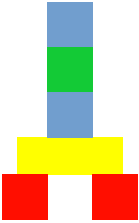
\includegraphics[scale=0.20]{figures/chapter2/task_goal.pdf}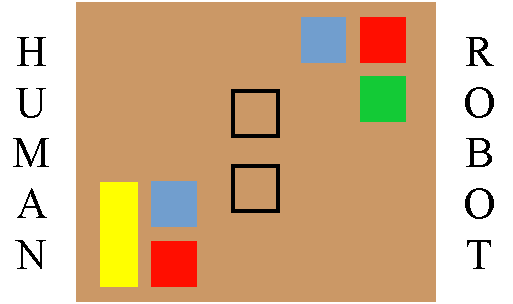
\includegraphics[scale=0.18]{figures/chapter2/task_setup_mini.pdf}}   
	\fancyhead[RO]{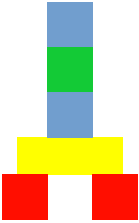
\includegraphics[scale=0.20]{figures/chapter2/task_goal.pdf}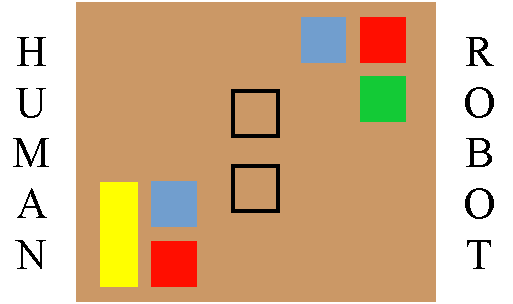
\includegraphics[scale=0.18]{figures/chapter2/task_setup_mini.pdf}\bfseries\thepage}  
	\fancyhead[RE]{\bfseries\nouppercase{\leftmark}}      % Chapter in the right on even pages
	\fancyhead[LO]{\bfseries\nouppercase{\rightmark}}     % Section in the left on odd pages
}%

\usepackage{pdfpages}
\usepackage{makecell}
\usepackage{pdflscape} 
\usepackage{mathtools}
\usepackage[section]{placeins}
\usepackage{afterpage}

%%%%%%%% my commands
\newcommand{\etal}{\textit{et al}.}
\newcommand{\ie}{\textit{i.e.}, }
\newcommand{\eg}{\textit{e.g.}, }
\newcommand{\fact}[3]{\mbox{\textit{#1}(#2, #3)}}
\newcommand{\circledtext}[1]{\raisebox{.5pt}{\textcircled{\raisebox{-.9pt} {#1}}}}
\newcommand{\sparql}{\textsc{SPARQL}}

\newcommand{\algConst}[1]{${\scriptscriptstyle #1}$}
\newcommand{\algNormTextSub}[2]{$\text{#1}_{#2}$}

\newcommand{\aslnumber}[1]{$#1$}
\newcommand{\aslstring}[1]{\textsf{#1}}
\newcommand{\aslvar}[1]{\textcolor{purple}{\textit{#1}}}
\newcommand{\asllabel}[1]{\textbf{#1}}
\newcommand{\annotation}[1]{{\footnotesize #1}}
\newcommand{\rulebody}[1]{\mbox{\hspace{.05\linewidth}}\begin{minipage}[t]{0.9\linewidth}#1.\end{minipage}}
\newcommand{\context}[1]{\begin{minipage}[t]{0.9\linewidth}#1\end{minipage}}
\newcommand{\planbody}[1]{\begin{minipage}[t]{0.9\linewidth}#1.\end{minipage}}
\newcommand{\Jason}[0]{\textbf{\textit{Jason}}}
\newcommand{\sn}{\mbox{\large\textbf{\texttt{\textasciitilde}}}}


\usepackage[acronym]{glossaries}

\makenoidxglossaries

\newacronym{bdi}{BDI}{Belief-Desire-Intention}
\newacronym{hateb}{HATEB}{Human-Aware Timed Elastic Bands}
\newacronym{hri}{HRI}{Human Robot Interaction}
\newacronym{hci}{HCI}{Human Computer Interaction}
\newacronym{jahrvis}{JAHRVIS}{Joint Action-based Human-Aware supeRVISor}
\newacronym{htn}{HTN}{Hierarchical Task Network}
\newacronym{hatp}{HATP}{Hierarchical Agent-based Task Planner}
\newacronym{reg}{REG}{Referring Expression Generation}
\newacronym{re}{RE}{Referring Expression}
\newacronym{teb}{TEB}{Timed Elastic Band}
\newacronym{kb}{KB}{Knowledge Base}
\newacronym{mummer}{MuMMER}{MultiModal Mall Entertainment Robot}
\newacronym{clle}{CLLE}{Cognition, Langues, Langage, Ergonomie}
\newacronym{ttc}{TTC}{Time-to-Collision}
\newacronym{ux}{UX}{User Experience}
\newacronym{perdita}{PeRDITA}{Pertinence of Robot Decisions In joinT Action}
\newacronym{hatpehda}{HATP/EHDA}{Human Aware Task Planner with Emulation of Human Decisions and Actions}
\newacronym{ssr}{SSR}{Semantic Spatial Representation}
\newacronym{rja}{RJA}{ROS-Jason Agent}
\newacronym{ham}{HAM}{Human Actions Monitoring}
\newacronym{hpm}{HPM}{Human Plan Manager}
\newacronym{tom}{ToM}{Theory of Mind}

%\nomenclature[A]{$\realset$}{Real Numbers}
%\nomenclature[A]{$\intset$}{Natural Numbers}
%
%\nomenclature[G]{$\robotmodel$}{The generic model of the robot has of itself. It can include action models or knowledge}
%\nomenclature[G]{$\humanmodel$}{The generic model of the human given to the robot. It can include action models or knowledge}
%\nomenclature[G]{$\robotinhumanmodel$}{The generic estimation of the model of the robot the human has. It can include action models or knowledge}
%
%\nomenclature[N]{$\robotband$}{The robot elastic band used in HATEB}
%\nomenclature[N]{$\humanband$}{The human elastic band used in HATEB}
%
%\nomenclature[O]{$\knowledgebase$}{The knowledge base (ontology)}
%\nomenclature[O]{$\abox$}{The ABox of the ontology}
%\nomenclature[O]{$\tbox$}{The TBox of the ontology}
%\nomenclature[O]{$\rbox$}{The RBox of the ontology}
%\nomenclature[O]{$\indivset$}{The set of entities in the ontology}
%\nomenclature[O]{$\classset$}{The set of classes in the ontology}
%\nomenclature[O]{$\relationset$}{The set of relations in the ontology}
%\nomenclature[O]{$\relationset$}{The set of relations in the ontology}
%
%\nomenclature[R]{$\variableset$}{The set of variables used in the \sparql{} queries and in referring expressions}
%\nomenclature[R]{$\labelfunc$}{The labeling function}
%\nomenclature[R]{$\costcompfunc$}{The properties interpretation cost function}
%\nomenclature[R]{$\goalindiv$}{The target entity, the entity to generate a referring expression for}
%\nomenclature[R]{$\usablepropset$}{The set of usable properties for the referring expression generation problem}
%\nomenclature[R]{$\regproblem$}{The referring expression generation problem}
%\nomenclature[R]{$\node$}{A node of the search space graph for the referring expression generation}
%\nomenclature[R]{$\transition$}{A transition of the search space graph for the referring expression generation}
%\nomenclature[R]{$\softdiff$}{The soft difference function, returning a list of relations from two entities}
%\nomenclature[R]{$\harddiff$}{The hard difference function, returning a list of relations from two entities}
%
%\nomenclature[Z]{$\statespace$}{The set of all the possible world states (beliefs)}
%\nomenclature[Z]{$\agents$}{The set of the agents (controllable and uncontrollable) considered during the planning}
%\nomenclature[Z]{$\agentstate$}{A state of an agent, containing their agenda, (partial) plan and beliefs}
%\nomenclature[Z]{$\ctrlagents$}{The set of controllable agents (robots)}
%\nomenclature[Z]{$\unctrlagents$}{The set of uncontrollable agents (humans)}
%\nomenclature[Z]{$\agentsstates$}{The union of the state of all the agents considered by the planner}
%\nomenclature[Z]{$\agentsstatesset$}{The set of all the possible states of all the agents considered by the planner}
%\nomenclature[Z]{$\actionmodel$}{The action model of an agent}
%\nomenclature[Z]{$\operators$}{The set of primitive tasks of an agent}
%\nomenclature[Z]{$\abstracttasks$}{The set of abstract tasks of an agent}
%\nomenclature[Z]{$\methods$}{The set of methods of an agent}
%\nomenclature[Z]{$\agenda$}{The agenda of an agent}
%\nomenclature[Z]{$\plan$}{The (partial) plan (execution stream) of an agent}
%\nomenclature[Z]{$\triggerset$}{The set of trigger functions of an agent}
%\nomenclature[Z]{$\Pi$}{A conditional plan}

%\nomenclature{HRI}{Human Robot Interaction}
%\nomenclature{REG}{Referring Expression Generation}
%\nomenclature{RE}{Referring Expression}
%\nomenclature{TEB}{Timed Elastic Band}
%\nomenclature{HATEB}{Human-Aware Timed Elastic Bands}

\usepackage{xargs}                      % Use more than one optional parameter in a new commands
\usepackage{xcolor}  % Coloured text etc.
% 
%\usepackage[colorinlistoftodos,prependcaption,textsize=tiny]{todonotes}
\usepackage[disable,colorinlistoftodos,prependcaption,textsize=tiny]{todonotes}
\setlength{\marginparwidth}{3cm}
\newcommandx{\unsure}[2][1=]{\todo[linecolor=red,backgroundcolor=red!25,bordercolor=red,#1]{#2}}
\newcommandx{\change}[2][1=]{\todo[linecolor=blue,backgroundcolor=blue!25,bordercolor=blue,#1]{#2}}
\newcommandx{\info}[2][1=]{\todo[linecolor=olive,backgroundcolor=olive!25,bordercolor=olive,#1]{#2}}
\newcommandx{\improvement}[2][1=]{\todo[linecolor=violet,backgroundcolor=violet!25,bordercolor=violet,#1]{#2}}
\newcommandx{\thiswillnotshow}[2][1=]{\todo[disable,#1]{#2}}


%%%%%
% À mettre dans le préambule (avant \begin{document})
%%%%%
%% Titre, auteur, date, laboratoire, cotutelle
\title{Endowing the Robot with the Abilities to Control and Evaluate its Contribution to a Human-Robot Joint Action}
\author{Amandine MAYIMA}
\defencedate{29/10/2021}
\lab{Laboratoire d'Analyse et d'Architecture des Systèmes (LAAS-CNRS)}
%\cotutelle{Institut de cotutelle}

%% Directeur(s) de thèse
\nboss{2}                                    % Nombre de directeur(s) de thèse
\makesomeone{boss}{2}{Aurélie CLODIC}{}{}  % Sera affiché en second
\makesomeone{boss}{1}{Rachid ALAMI}{}{} % Sera affiché en premier
%% Referee
\nreferee{2}
\makesomeone{referee}{1}{Silvia ROSSI}{}{}
\makesomeone{referee}{2}{Peter Ford DOMINEY}{}{}
%% Jury
\njudge{7}
%\makesomeone{judge}{1}{???}{Professeur}{Président du Jury}
\makesomeone{judge}{2}{Silvia ROSSI}{Professeure Associée}{Rapporteure}
\makesomeone{judge}{3}{Peter Ford DOMINEY}{Directeur de Recherche}{Rapporteur}
\makesomeone{judge}{7}{Rachid ALAMI}{Directeur de Recherche}{Directeur de Thèse}
\makesomeone{judge}{6}{Aurélie CLODIC}{Ingénieure de Recherche}{Directrice de Thèse}
\makesomeone{judge}{1}{Simon LACROIX}{Directeur de Recherche}{Président du Jury}
\makesomeone{judge}{4}{Guy HOFFMAN}{Professeur Associé}{Membre du Jury}
\makesomeone{judge}{5}{Elisabeth PACHERIE}{Directrice de Recherche}{Membre du Jury}
%% Quel ordre ?

\sloppy
\begin{document}
\lstMakeShortInline[columns=fixed,breaklines=false]|
\makeflyleaf

\cleardoublepage

\dominitoc

\pagenumbering{roman}

 \cleardoublepage


\chapter*{Abstract}
%%%%%%%%%%%%%%%%%%%%%% ATTENTION  ! SI MODIFICATION => MODIF SUR ADUM AUSSI !!!

Robots will interact more and more with humans in the future and thus will need to be endowed with the pertinent abilities. We are still far from having autonomous robots among humans and able to smoothly collaborate with them but, the work of this thesis is a contribution bringing the community a bit closer to this goal. 

When humans collaborate to achieve a task together, numerous cognitive mechanisms come into play, more than we would have thought at first glance. Some of these mechanisms are also triggered in humans’ minds when they interact with robots as they are essential to a successful collaboration. Therefore, it is important for roboticists designing robots that will closely interact with humans to be aware of and consider the humans mental states and sensorimotor functions involved in controlling and smoothing collaborative task performance. However, this does not imply that robots have to be endowed with the same mechanisms since being able to collaborate with humans does not mean to imitate them. What is key to roboticists is to understand how humans work and to design  robots that will adapt. 

Consequently, this thesis starts with an immersion in philosophy and social and cognitive psychology. Then, we explore \acrfull{bdi} and cognitive robotic architectures  which have inspired us to design our own architecture in which, \acrshort{jahrvis} —  the main contribution of this thesis — endows a robot with the abilities not only to control, but also to evaluate its joint action with a human. 

\acrfull{jahrvis} is what we call a supervision system, \ie it embeds the robot high-level decisions, controls its behavior and tries to react to contingencies, always considering the human it is interacting with. It is able to do so by taking into account shared plans, human mental states, its knowledge about the current state of the environment, and human actions. \acrshort{jahrvis} is designed in such a way that it is generic enough to handle various kinds of tasks. 

Not only \acrshort{jahrvis} controls the robot contribution to a collaborative task, but it also tries to evaluate if the interaction is going well or not. It is possible thanks to a set of metrics we have built and a method to aggregate them. We claim that having a robot with this ability allows it to enhance and make more pertinent its decision-making processes. In future work, this granularity will allow the robot to know precisely on what level it needs to act when a low \acrlong{qoi} is assessed. 

\acrshort{jahrvis} has been integrated in a cognitive robotic architecture and effectively deployed to achieve several collaborative and service tasks. These tasks demonstrated the robot’s abilities related to perspective-taking, planning, knowledge representation with theory of mind, manipulation, and communication.

\clearpage

\chapter*{Résumé}
%%%%%%%%%%%%%%%%%%%%%% ATTENTION  ! SI MODIFICATION => MODIF SUR ADUM AUSSI !!!

Dans le futur, les robots interagiront chaque jour un peu plus avec les humains et devront donc être dotés des capacités adéquates. Nous sommes encore loin de robots autonomes parmi les humains, capables de collaborer sans problème avec eux : le travail de cette thèse est une contribution qui rapproche un peu plus la communauté de cet objectif. 


Lorsque des personnes collaborent pour réaliser une tâche ensemble, de nombreux mécanismes cognitifs entrent en jeu, plus qu’il n’y paraît à première vue. Certains de ces mécanismes sont aussi activés quand un humain interagit avec un robot et non plus avec un autre humain, car ils sont essentiels à une collaboration réussie. Il est donc important que les roboticiens qui conçoivent des robots destinés à interagir étroitement avec les humains soient conscients de cela et qu’ainsi ils prennent en compte les états mentaux des humains et les fonctions sensori-motrices impliquées dans le contrôle et la fluidité de l'exécution des tâches collaboratives. Toutefois, cela ne signifie pas que les robots doivent être dotés de ces mêmes mécanismes, car être capable de collaborer avec les humains ne signifie pas les imiter. Ce qui est essentiel pour les roboticiens, c'est de comprendre comment les humains travaillent et de concevoir des robots qui s'adapteront. 


Ce manuscrit commence par une immersion dans la philosophie et la psychologie. Ensuite, nous explorons les modèles ``croyance-désir-intention'' et les architectures robotiques cognitives qui nous ont inspirés pour concevoir notre propre architecture dans laquelle, \acrshort{jahrvis} -- la principale contribution de cette thèse -- au robot de, non seulement contrôler, mais aussi d'évaluer son action jointe avec un humain. 

\acrfull{jahrvis} est ce que nous appelons un système de supervision, \ie il prend les décisions haut niveau du robot, contrôle son comportement et tente de réagir aux imprévus, en tenant toujours compte de l'humain avec lequel il interagit. Il peut le faire en se basant sur les plans partagés qu’il génère, sa connaissance des états mentaux de l'humain et de l'état actuel de l'environnement et, les actions de l'humain. \acrshort{jahrvis} est conçu de manière à être suffisamment générique pour gérer différents types de tâches.

\acrshort{jahrvis} ne se contente pas de contrôler la contribution du robot à une tâche collaborative, il essaie également d'évaluer si l'interaction se déroule bien ou non. C'est possible grâce à un ensemble de métriques et à une méthode pour les agréger que nous avons conçus. Nous affirmons que le fait de doter un robot de cette capacité lui permet d'améliorer et de rendre plus pertinent son processus de prise de décision. Dans les travaux futurs, cette granularité permettra au robot de savoir à quel niveau il doit agir lorsqu'une faible Qualité d'Interaction est évaluée.

\acrshort{jahrvis} a été intégré dans une architecture robotique cognitive et déployé efficacement pour réaliser plusieurs tâches collaboratives. Elles ont démontré les capacités du robot en matière de prise de perspective, de planification, de représentation des connaissances avec la théorie de l'esprit, de manipulation et de communication.


% Here you can see an example of how to create text conditioned by the language
% variable. The \iftoggle command:
%
%   \iftoggle{ThesisInEnglish}{%
%   <your-text-in-english>
%   }{%
%   <your-text-in-french>
%   }
%
% will compile only one of the two blocks, depending on the variable you set at
% the beginning of this document. Language selection is managed this way in the
% formatAndDefs.tex file. You too can create sections of your thesis that is
% language dependend this way, although you probably won't need it. Another use
% of \iftoggle can be found at the end of this file.

\selectlanguage{french}
\chapter*{Remerciements}


Ces quelques mots, j'écris\\
Car touche maintenant à sa fin,\\
Ce qui a semblé être un long chemin.\\
Il est maintenant temps, de dire merci.\\
\\
Merci à Aurélie Clodic,\\
Pour sa foi inébranlable,\\
Elle fut un soutien indispensable,\\
Pour ôter de ma thèse, l'aspect chimérique.\\
\\
Merci à Rachid Alami,\\
De m'avoir poussé, donné cette opportunité,\\
Pour son intarissable flot d'idées,\\
De cela, je me suis continuellement nourri.\\
\\
Merci à Simon Lacroix,\\
D'avoir, en Adream, laissé entrer la joie,\\
Et d'avoir rempli son rôle de vieux sage,\\
Prodiguant conseils et relisant mes pages.\\
\\
Merci à mon jury et mes rapporteurs,\\
Pour leur lecture, questionnement et avis.\\
Personnes dont le travail j'apprécie,\\
Qu'ils acceptent ces rôles fut un honneur.\\
\\
Merci aux Mousquetaires,\\
Professionnellement, amicalement, humainement.\\
Union formée dans les moments plus bas que terre,\\
Elle fut aussi témoin de moments d'enjouement.\\
\\
Merci à Guilhem Buisan,\\
Je repense encore à cet instant,\\
Où dehors je lui confiais mes malheurs,\\
Ce fut pour moi salvateur.\\
\\
Merci à Guillaume Sarthou,\\
Qui ne me fait plus peur (et encore que).\\
Notre collaboration fut pour moi un véritable atout,\\
Et ce, sans compter nos discussions et les jeux.\\
\\
Merci à Kathleen Belhassein,\\
De m'avoir ouverte les portes de l'action jointe,\\
Mais surtout pour cette amitié non feinte,\\
Nous permettant de partager nos joies et nos peines.\\
\\
Merci à Amelie Barozet,\\
Elle ne fut pas au labo sur toute la durée,\\
Mais ce n'est qu'un détail, nos soirées, goûters,\\
Et jeux de société n'y faisaient que commencer.\\
\\
Merci à Yannick Riou,\\
Dit l'ingénieur fidèle, garant des mouvements.\\
Savant mélange d'enthousiasme et râlements,\\
Ce fut un ravissement qu'il puisse être là jusqu'au bout.\\
\\
Merci à Ilinka Clerc,\\
Pour sa gentillesse à l'accoutumé,\\
Pour sa malice en jeux de société,\\
Ma petite protégée, mon héritière.\\
\\
Merci à Anthony, Antoine, Philippe, Jérémy, Phani et Rafa,\\
De l'open-space, ils furent de précieux compagnons,\\
Entrecoupant le travail de petites conversations.\\
Il n'aurait pas fallu qu'on me les échangea.\\
\\
Merci à Gianluca, Andrea et Dario,\\
Accompagnés de leur charmant accent,\\
Croisés au détour d'un couloir ou lors d'un pot,\\
Chaque moment fut un contentement.\\
\\
Merci à (Raph), Arthur, Alejandro, Ellon, Christophe, Sandra et Jules,\\
Ce sont ceux qui furent là au préambule.\\
\\
Merci à Smail, William, Valentin, Shashank, Eli et Simon,\\
Ce sont ceux qui furent là à la conclusion.\\
\\
Merci aussi à David, Pierre, Léa, Élise, Vivien, Sylvain,\\
Idriss, Paul, Tanguy, Jean-Hugues, Alexandre, Florian et Florian,\\
Ce sont ceux qui furent là un peu pendant.\\
\\
Merci aux permanents de l'équipe RIS,\\
Ce sont ceux qui furent là tout le temps.\\
\\
\\
Merci à ceux qui existent en dehors de RIS,\\
Communication, personnel et sysadmin, ces précieux services.\\
Merci à Sabrina,\\
Pour son implication, sa présence et son chocolat.\\
\\
Merci au personnel du CAES et au CAES,\\
De m'avoir permis de voyager dans l'allégresse,\\
De m'avoir permis de découvrir boxe, tir à l'arc, zumba et salsa,\\
Ces interludes bienvenus avec plein de gens sympas.\\
\\
Merci aux personnels des restaurants du LAAS, du central et du CROUS,\\
Pour leurs sourires et leur humeur douce.\\
\\
Merci à tous les enseignants,\\
Que j'ai croisé sur ma route.\\
Pensée spéciale à M. Durand,\\
Pour ne pas avoir eu de doutes.\\
\\
Merci à tous mes amis, ô que nombreux,\\
De m'avoir offert soutien et moments heureux,\\
D'avoir porté tant d'intérêt à mon sujet,\\
Et à ma soutenance, de m'avoir accompagné.\\
Entre autres, Siméon, Jeanne, Caroline, Coralie, Éric, Nicola,\\
Les habitants  du Lou Castel, Benoît, Ximun, Marie, Iban, Laura,\\
Cyril, Thibault, Vincent, Mathieu,  Philomène, Sarah, Alissa,\\
Alpha, Léa, Marine, Sarah, Sarah, Noëmie, Kim, Leïla.\\
\\
Merci à Estelle,\\
D'avoir contribué à mon enrichissement personnel,\\
Car elle a entre autre été, mon initiatrice aux jeux,\\
Ce qui fut un atout bienvenu dans mon milieu,\\
\\
Merci à ma mère,\\
De m'avoir ouvert tant de portes de genres divers,\\
Me laissant le choix d'y entrer ou de les refermer.\\
Plus qu'elle ne le sait et ne se l'admet, elle m'a donné.\\
\\
Merci à mon père,\\
D'avoir forgé ce caractère\\
N'acceptant pas le non et voulant toujours poursuivre,\\
Pour le meilleur et pour le pire.\\
\\
\\
\\
Merci à Bérénice,\\
Cette petite s\oe{}ur complice,\\
Parfois comme chien et chat,\\
Mais l'une et l'autre seront toujours là.\\
\\
Merci à Constantin,\\
Ce petit frère malin,\\
Moins bizarre qu'il ne le pense,\\
C'est un plaisir quand il honore de sa présence.\\
\\
Merci à mon oncle,\\
De m'avoir initié à l'informatique,\\
Ce n'est pas là un rôle quelconque,\\
Lorsque de cette thèse, on regarde la thématique.\\
\\
Merci à ma grand-mère,\\
Merci à ma presque grand-mère Françoise,\\
Merci à Farnesie, merci à mon oncle Roland,\\
Ainsi qu'au reste de cette immense famille congolaise,\\
Pensées pour mes grands-pères, tout là-haut.\\
\\
Merci à Miki,\\
D'avoir été un précieux contributeur,\\
Ma thèse ne serait pas ce qu'elle est sans lui.\\
Et merci d'être au quotidien, mon collaborateur.





\selectlanguage{english}

\tableofcontents

%\printnomenclature
\printnoidxglossary[type=\acronymtype]
% Use \mtcfixnomenclature below if you have a glossary (added with
% \printnomenclature above) and you're see a shift in the mini-table of
% contents at the begining of each chapter (example: no mini-toc in chapter 1;
% mini-toc of chapter 1 appearing in chapter 2; and so on).
%
% You should not use \mtcfixnomenclature if you have no glossary (that means,
% if you don't use \printnomenclature or if your glossary is empty).
%\mtcfixnomenclature



\mainmatter
\fancyhead[RE, LO]{\bfseries\nouppercase{Introduction}}
\ifdefined\included
\else
\documentclass[a4paper,11pt,twoside]{StyleThese}
\usepackage{amsmath,amssymb, amsthm}             % AMS Math
\usepackage[T1]{fontenc}
\usepackage[utf8x]{inputenc}
\usepackage{babel}
\usepackage{datetime}

\usepackage{silence}

\WarningFilter{minitoc(hints)}{W0023}
\WarningFilter{minitoc(hints)}{W0028}
\WarningFilter{minitoc(hints)}{W0030}

\usepackage{lmodern}
\usepackage{tabularx}
%\usepackage{tabular}
\usepackage{multirow}
\usepackage{xspace}

\usepackage{subfig}
\usepackage[inline]{enumitem}

\usepackage{hhline}
\usepackage[left=1.5in,right=1.3in,top=1.1in,bottom=1.1in,includefoot,includehead,headheight=13.6pt]{geometry}
\renewcommand{\baselinestretch}{1.05}

% Table of contents for each chapter

\usepackage[nottoc, notlof, notlot]{tocbibind}
\usepackage{minitoc}
\setcounter{minitocdepth}{2}
\mtcindent=15pt
% Use \minitoc where to put a table of contents

\usepackage{aecompl}

% Glossary / list of abbreviations

\usepackage[intoc]{nomencl}
\iftoggle{ThesisInEnglish}{%
\renewcommand{\nomname}{Glossary}
}{ %
\renewcommand{\nomname}{Liste des Abréviations}
}

\usepackage{etoolbox}
\renewcommand\nomgroup[1]{%
  \item[\bfseries
  \ifstrequal{#1}{A}{Number Sets}{%
  \ifstrequal{#1}{G}{Agents Beliefs and Action Models}{%
  \ifstrequal{#1}{N}{Navigation}{%
  \ifstrequal{#1}{O}{Ontology}{%
  \ifstrequal{#1}{R}{Referring Expression Generation}{%
  \ifstrequal{#1}{Z}{Controllable and Uncontrollable Agents Task Planning}{}}}}}}%
]}

\makenomenclature



% My pdf code

\usepackage{ifpdf}

\ifpdf
  \usepackage[pdftex]{graphicx}
  \DeclareGraphicsExtensions{.jpg}
  \usepackage[pagebackref,hyperindex=true]{hyperref}
  \usepackage{tikz}
  \usetikzlibrary{arrows,shapes,calc}
\else
  \usepackage{graphicx}
  \DeclareGraphicsExtensions{.ps,.eps}
  \usepackage[dvipdfm,pagebackref,hyperindex=true]{hyperref}
\fi

\graphicspath{{.}{images/}}

%% nicer backref links. NOTE: The flag ThesisInEnglish is used to define the
% language in the back references. Read more about it in These.tex

\iftoggle{ThesisInEnglish}{%
\renewcommand*{\backref}[1]{}
\renewcommand*{\backrefalt}[4]{%
\ifcase #1 %
(Not cited.)%
\or
(Cited in page~#2.)%
\else
(Cited in pages~#2.)%
\fi}
\renewcommand*{\backrefsep}{, }
\renewcommand*{\backreftwosep}{ and~}
\renewcommand*{\backreflastsep}{ and~}
}{%
\renewcommand*{\backref}[1]{}
\renewcommand*{\backrefalt}[4]{%
\ifcase #1 %
(Non cité.)%
\or
(Cité en page~#2.)%
\else
(Cité en pages~#2.)%
\fi}
\renewcommand*{\backrefsep}{, }
\renewcommand*{\backreftwosep}{ et~}
\renewcommand*{\backreflastsep}{ et~}
}

% Links in pdf
\usepackage{color}
\definecolor{linkcol}{rgb}{0,0,0.4} 
\definecolor{citecol}{rgb}{0.5,0,0} 
\definecolor{linkcol}{rgb}{0,0,0} 
\definecolor{citecol}{rgb}{0,0,0}
% Change this to change the informations included in the pdf file

\hypersetup
{
bookmarksopen=true,
pdftitle="Endowing the robot with the abilities to control and evaluate its contribution to a human-robot joint action",
pdfauthor="Amandine MAYIMA", %auteur du document
pdfsubject="Thèse", %sujet du document
%pdftoolbar=false, %barre d'outils non visible
pdfmenubar=true, %barre de menu visible
pdfhighlight=/O, %effet d'un clic sur un lien hypertexte
colorlinks=true, %couleurs sur les liens hypertextes
pdfpagemode=None, %aucun mode de page
pdfpagelayout=SinglePage, %ouverture en simple page
pdffitwindow=true, %pages ouvertes entierement dans toute la fenetre
linkcolor=linkcol, %couleur des liens hypertextes internes
citecolor=citecol, %couleur des liens pour les citations
urlcolor=linkcol %couleur des liens pour les url
}

% definitions.
% -------------------

\setcounter{secnumdepth}{3}
\setcounter{tocdepth}{2}

% Some useful commands and shortcut for maths:  partial derivative and stuff

\newcommand{\pd}[2]{\frac{\partial #1}{\partial #2}}
\def\abs{\operatorname{abs}}
\def\argmax{\operatornamewithlimits{arg\,max}}
\def\argmin{\operatornamewithlimits{arg\,min}}
\def\diag{\operatorname{Diag}}
\newcommand{\eqRef}[1]{(\ref{#1})}

\usepackage{rotating}                    % Sideways of figures & tables
%\usepackage{bibunits}
%\usepackage[sectionbib]{chapterbib}          % Cross-reference package (Natural BiB)
%\usepackage{natbib}                  % Put References at the end of each chapter
                                         % Do not put 'sectionbib' option here.
                                         % Sectionbib option in 'natbib' will do.
\usepackage{fancyhdr}                    % Fancy Header and Footer

% \usepackage{txfonts}                     % Public Times New Roman text & math font
  
%%% Fancy Header %%%%%%%%%%%%%%%%%%%%%%%%%%%%%%%%%%%%%%%%%%%%%%%%%%%%%%%%%%%%%%%%%%
% Fancy Header Style Options

\pagestyle{fancy}                       % Sets fancy header and footer
\fancyfoot{}                            % Delete current footer settings

%\renewcommand{\chaptermark}[1]{         % Lower Case Chapter marker style
%  \markboth{\chaptername\ \thechapter.\ #1}}{}} %

%\renewcommand{\sectionmark}[1]{         % Lower case Section marker style
%  \markright{\thesection.\ #1}}         %

\fancyhead[LE,RO]{\bfseries\thepage}    % Page number (boldface) in left on even
% pages and right on odd pages
\fancyhead[RE]{\bfseries\nouppercase{\leftmark}}      % Chapter in the right on even pages
\fancyhead[LO]{\bfseries\nouppercase{\rightmark}}     % Section in the left on odd pages

\let\headruleORIG\headrule
\renewcommand{\headrule}{\color{black} \headruleORIG}
\renewcommand{\headrulewidth}{1.0pt}
\usepackage{colortbl}
\arrayrulecolor{black}

\fancypagestyle{plain}{
  \fancyhead{}
  \fancyfoot{}
  \renewcommand{\headrulewidth}{0pt}
}

%\usepackage{MyAlgorithm}
%\usepackage[noend]{MyAlgorithmic}
\usepackage{algorithm}
\usepackage[noend]{algpseudocode}
\usepackage{comment}
\usepackage[ED=MITT-InfoTel, Ets=INSA]{tlsflyleaf}
%%% Clear Header %%%%%%%%%%%%%%%%%%%%%%%%%%%%%%%%%%%%%%%%%%%%%%%%%%%%%%%%%%%%%%%%%%
% Clear Header Style on the Last Empty Odd pages
\makeatletter

\def\cleardoublepage{\clearpage\if@twoside \ifodd\c@page\else%
  \hbox{}%
  \thispagestyle{empty}%              % Empty header styles
  \newpage%
  \if@twocolumn\hbox{}\newpage\fi\fi\fi}

\newcommand*{\algrule}[1][\algorithmicindent]{%
	\makebox[#1][l]{%
		\hspace*{.2em}% <------------- This is where the rule starts from
		\vrule height .75\baselineskip depth .25\baselineskip
	}
}

%%% to have lines in algorithm, from stackexchange
\newcount\ALG@printindent@tempcnta
\def\ALG@printindent{%
	\ifnum \theALG@nested>0% is there anything to print
	\ifx\ALG@text\ALG@x@notext% is this an end group without any text?
	% do nothing
	\else
	\unskip
	% draw a rule for each indent level
	\ALG@printindent@tempcnta=1
	\loop
	\algrule[\csname ALG@ind@\the\ALG@printindent@tempcnta\endcsname]%
	\advance \ALG@printindent@tempcnta 1
	\ifnum \ALG@printindent@tempcnta<\numexpr\theALG@nested+1\relax
	\repeat
	\fi
	\fi
}
% the following line injects our new indent handling code in place of the default spacing
\patchcmd{\ALG@doentity}{\noindent\hskip\ALG@tlm}{\ALG@printindent}{}{\errmessage{failed to patch}}
\patchcmd{\ALG@doentity}{\item[]\nointerlineskip}{}{}{} % no spurious vertical space
% end vertical rule patch for algorithmicx

\makeatother
 
%%%%%%%%%%%%%%%%%%%%%%%%%%%%%%%%%%%%%%%%%%%%%%%%%%%%%%%%%%%%%%%%%%%%%%%%%%%%%%% 
% Prints your review date and 'Draft Version' (From Josullvn, CS, CMU)
\newcommand{\reviewtimetoday}[2]{\special{!userdict begin
    /bop-hook{gsave 20 710 translate 45 rotate 0.8 setgray
      /Times-Roman findfont 12 scalefont setfont 0 0   moveto (#1) show
      0 -12 moveto (#2) show grestore}def end}}
% You can turn on or off this option.
% \reviewtimetoday{\today}{Draft Version}
%%%%%%%%%%%%%%%%%%%%%%%%%%%%%%%%%%%%%%%%%%%%%%%%%%%%%%%%%%%%%%%%%%%%%%%%%%%%%%% 

\newenvironment{maxime}[1]
{
\vspace*{0cm}
\hfill
\begin{minipage}{0.5\textwidth}%
%\rule[0.5ex]{\textwidth}{0.1mm}\\%
\hrulefill $\:$ {\bf #1}\\
%\vspace*{-0.25cm}
\it 
}%
{%

\hrulefill
\vspace*{0.5cm}%
\end{minipage}
}

\let\minitocORIG\minitoc
\renewcommand{\minitoc}{\minitocORIG \vspace{1.5em}}

\usepackage{multirow}
%\usepackage{slashbox}

\newenvironment{bulletList}%
{ \begin{list}%
	{\tiny$\bullet$}%
	{\setlength{\labelwidth}{25pt}%
	 \setlength{\leftmargin}{30pt}%
	 \setlength{\itemsep}{-0.5em}}}%
{ \end{list} }

\newenvironment{inlineEnumerate}
{\begin{enumerate*} [label={(\arabic*)}] }
{\end{enumerate*}}

\theoremstyle{definition}
\newtheorem{definition}{Definition}
\renewcommand{\epsilon}{\varepsilon}

% centered page environment

\newenvironment{vcenterpage}
{\newpage\vspace*{\fill}\thispagestyle{empty}\renewcommand{\headrulewidth}{0pt}}
{\vspace*{\fill}}

\newenvironment{asl}{\ttfamily\begin{tabbing}~~~\=$\leftarrow$ \= ~~~ \=
		\kill}{\end{tabbing}}

\usepackage{tablefootnote}

\theoremstyle{plain}
\newtheorem{constraint}{Constraint}[section]

\algnewcommand\algorithmicforeach{\textbf{for each}}
\algnewcommand\algorithmicin{\textbf{in}}
\algdef{S}[FOR]{ForEach}[2]{\algorithmicforeach\ #1\ \algorithmicin\ #2\ \algorithmicdo}

\algnewcommand\algorithmicforkxor{\textbf{do fork-join-xor}}
\algnewcommand\algorithmicendforkxor{\textbf{end fork-join-xor}}
\algdef{SE}{ForkXor}{EndForkXor}{\algorithmicforkxor}{\algorithmicendforkxor}


\usepackage{listings}
\lstset{
	frame=single,
	captionpos=b,
	breaklines=true,
	basicstyle=\ttfamily,
	numberstyle=\color{black},
	tabsize=2,
	mathescape=true,
	literate=%
		{â}{{\^a}}1
}

\lstdefinestyle{inline}{
	frame=none,
	aboveskip=\smallskipamount,
	belowskip=\smallskipamount,
}

\lstdefinestyle{OwlTurtle}{
	language=C,
	tabsize=4,
	basicstyle=\scriptsize\ttfamily,
	keywordstyle=\bfseries\color{darkgray},
	morekeywords={rdf:type, rdfs:domain, rdfs:subPropertyOf, rdfs:range, :hasSubtask, :DecompositionUsedBy, rdfs:subClassOf, :hasDecomposition, owl:inverseOf, htn_actions:hasEffect, rdfs:label},
	alsoletter=:
}

\lstdefinestyle{aslDef}{
	frame=none,
%	breaklines=false,
	%xleftmargin=.1\textwidth, xrightmargin=.1\textwidth
}

\fancypagestyle{example}{%
	\fancyhead[LE]{\bfseries\thepage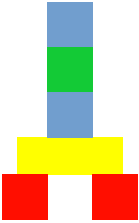
\includegraphics[scale=0.20]{figures/chapter2/task_goal.pdf}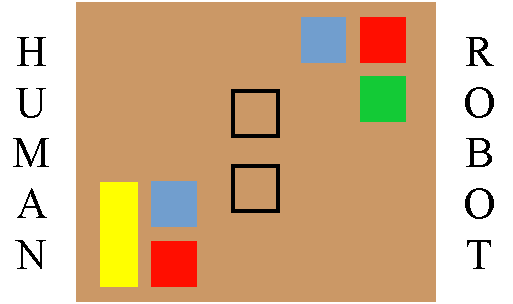
\includegraphics[scale=0.18]{figures/chapter2/task_setup_mini.pdf}}   
	\fancyhead[RO]{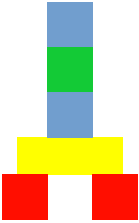
\includegraphics[scale=0.20]{figures/chapter2/task_goal.pdf}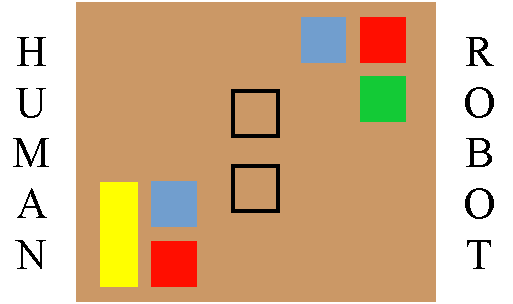
\includegraphics[scale=0.18]{figures/chapter2/task_setup_mini.pdf}\bfseries\thepage}  
	\fancyhead[RE]{\bfseries\nouppercase{\leftmark}}      % Chapter in the right on even pages
	\fancyhead[LO]{\bfseries\nouppercase{\rightmark}}     % Section in the left on odd pages
}%

\usepackage{pdfpages}
\usepackage{makecell}
\usepackage{pdflscape} 
\usepackage{mathtools}
\usepackage[section]{placeins}
\usepackage{afterpage}

%%%%%%%% my commands
\newcommand{\etal}{\textit{et al}.}
\newcommand{\ie}{\textit{i.e.}, }
\newcommand{\eg}{\textit{e.g.}, }
\newcommand{\fact}[3]{\mbox{\textit{#1}(#2, #3)}}
\newcommand{\circledtext}[1]{\raisebox{.5pt}{\textcircled{\raisebox{-.9pt} {#1}}}}
\newcommand{\sparql}{\textsc{SPARQL}}

\newcommand{\algConst}[1]{${\scriptscriptstyle #1}$}
\newcommand{\algNormTextSub}[2]{$\text{#1}_{#2}$}

\newcommand{\aslnumber}[1]{$#1$}
\newcommand{\aslstring}[1]{\textsf{#1}}
\newcommand{\aslvar}[1]{\textcolor{purple}{\textit{#1}}}
\newcommand{\asllabel}[1]{\textbf{#1}}
\newcommand{\annotation}[1]{{\footnotesize #1}}
\newcommand{\rulebody}[1]{\mbox{\hspace{.05\linewidth}}\begin{minipage}[t]{0.9\linewidth}#1.\end{minipage}}
\newcommand{\context}[1]{\begin{minipage}[t]{0.9\linewidth}#1\end{minipage}}
\newcommand{\planbody}[1]{\begin{minipage}[t]{0.9\linewidth}#1.\end{minipage}}
\newcommand{\Jason}[0]{\textbf{\textit{Jason}}}
\newcommand{\sn}{\mbox{\large\textbf{\texttt{\textasciitilde}}}}


\sloppy
\begin{document}
\fi


\chapter*{Introduction}
\addstarredchapter{Introduction} %Sinon cela n'apparait pas dans la table des matières
\markboth{INTRODUCTION}{}

Robots will interact more and more with humans in the future and thus will need to be endowed with the pertinent abilities. We are still far from having autonomous robots among humans and able to smoothly collaborate with them.

A lot of research focus on abilities needed to the robot to make it more intelligent, useful and adaptive: the planning, the perception, the knowledge management, the navigation, the action recognition, the dialog... But those does not make a robot function, those does not make a robot collaborate with a human in a task. What does? The supervision. Indeed, this component, such a puppeteer, controls from above the wires of the other architecture components. Leaning on them, it makes the decisions about how and when the robot should act, in a collaborative task with a human, it decides what the robot should say; reacting to the environment, the human behavior and the human speech. A robot should be able to act following a plan but more importantly, it should be able to react to the unexpected or to (robotic or human) errors. And what can give a robot such abilities? A supervision component, or we should say, a component with a vision.

Thereby, given the central role of this component, we could thought that it is extensively studied in \acrlong{hri}, a field of research whose aims is to build robots that will autonomously interact with humans. However, it is not. This lack led to a slight change of subject for this thesis. Indeed, initially, the goal was to devise a supervisor making the robot robust to a number of contingencies that could happen during a human-robot interaction. But, in order to have a supervisor handling contingencies, we needed first a supervisor for ``non-contingent'' situations. Well, we could not find any existing system implementing a supervision component in the context of human-robot collaborative tasks, on which we could build contingencies handling. Thus, we devised it.

\section*{A Supervision for \acrlong{hri}}
\markright{A Supervision for \acrlong{hri}}
When humans collaborate to achieve a task together, numerous neurocognitive mechanisms come into play, more than we would have thought at first glance. Some of these mechanisms are also triggered in humans’ minds when they interact with robots as they are essential to a successful collaboration. Therefore, it is important for roboticists designing robots that will closely interact with humans to be aware of and take into account the humans mental states and sensori-motor functions involved in controlling and smoothing collaborative task performance. However, this does not imply that robots have to be endowed with the same mechanisms since being able to collaborate with humans does not mean to imitate them. What is key to roboticists is to understand how humans work and to design  robots that will adapt. Consequently, we closely collaborated with a psychologist and a philosopher in order to learn the keys of human collaboration such as joint action, commitment, shared representations...(Chapter~\ref{chapter:chap1}) It was also back and forth discussions between them and us, trying to close the gap between what abilities a robot should have and what is currently technically possible.

Thus, when designing and implementing our supervisor for human-robot collaborative tasks, our minds were well nourished. In this thesis, we tackled the issue of a real component supervision for \acrshort{hri}. It endows the robot with a number of abilities in order to make the robot the best partner possible for humans such as modeling their mental states or adapting to their decisions (Chapter~\ref{chapter:chap5} and Chapter~\ref{chapter:chap6}).

\section*{A first step toward contingency handling}
\markright{A first step toward contingency handling}

Even though we could not lean on an existing supervision system in order to endow a robot with abilities making it able to cope with the unexpected, we started brainstorming on the subject. We realized that before being able to handle with contingencies, the robot should be able notice them. But, is it necessary to react immediately when something derails a bit or should there be a kind of threshold? As humans, sometimes, we run into minor incidents when performing a task for example, but as the situation is good overall, we tolerate it. Thus, we came with a novel idea: to give the robot the ability to evaluate, in real-time, the quality of its interaction with its human partner (Chapter~\ref{chapter:chap7}). This is a first step toward contingency handling as later, outside the scope of this thesis, it could integrated to the supervision, helping it to improve its decision and its reactions. For example, if something would go wrong during an action but the overall interaction quality was good, it could decide that it was not a matter of importance and ignore it. However, if it happened in the context of a bad quality or that the same action was going wrong again and again, then it could react.

\section*{Summary of the Thesis}
\markright{SUMMARY OF THE THESIS}

This manuscript is divided in four parts. 

The first part lays the funding principles of a decision-making system for human-robot collaboration. We start in Chapter~\ref{chapter:chap1} by providing a framework for reflecting upon key elements for human-human collaboration. We dive into psychology and philosophy literatures tackling multiple concepts, mainly around joint action such as shared representations, joint attention, coordination... But we also address social interactions, \acrlong{tom} and communication. 

Then, in Chapter~\ref{chapter:chap2}, we explore existing robotic systems implementing concepts associated to social interactions or joint action.

\bigskip 

The second part aims at presenting the key challenges of social interaction management. The supervision component belongs to a robotic architecture. Thus, in Chapter~\ref{chapter:chap3}, we present a number of robotic architectures and the one we integrated our component with. 

Then we highlight, in Chapter~\ref{chapter:chap4}, the central role of the supervision in this architecture as well as what tools are available to develop such a component and which one we chose.

\bigskip

In the third part are concentrated the two main contributions of this thesis: \acrfull{jahrvis}, the supervisor we devised, and a \acrfull{qoi} Evaluator. We start with an overview of the \acrshort{jahrvis} features in Chapter~\ref{chapter:chap5}, \ie a system embedding the robot high-level decisions, controlling its behavior, always considering the human it is interacting with. It is able to do so by taking into account shared plans, human mental states, its knowledge about the current state of the environment, and human actions, inspired by the principles described in Part~\ref{part:part1}. 

Then, we detail in Chapter~\ref{chapter:chap6}, one by one, the modules composing its structure: interaction management, human action recognition, shared plan handling, action execution management and communication management. It is accompanied with an example which has been executed on a PR2 robot. 

And, we introduce in Chapter~\ref{chapter:chap7}, a mean to evaluate from the robot point of view, the \acrlong{qoi}. We present the general concept, a set of metrics enabling such an ability and a way to aggregate these metrics. 

\bigskip

Finally, the fourth part present two tasks which have been executed thanks to the supervisor developed in the context of this thesis. The first task, presented in Chapter~\ref{chapter:chap8}, was tackled with the first version of \acrshort{jahrvis} in the context of a H2020 European project, \acrfull{mummer}\footnote{The \acrshort{mummer} project funded three years of this thesis out of four.}. The robot had to give directions to customers within a Finnish mall. This was a real challenge as the robot was deployed there for three months.

Lastly, in Chapter~\ref{chapter:chap9}, we present a task which was executed with the almost-complete version of \acrshort{jahrvis}. It is a task where a human and a robot partners have to communicate in order to remove the right cubes of a task. It was inspired by a task in psychology. We propose this task to the \acrshort{hri} community as a set of challenges to take up as well as a breeding ground for user studies.

\subsection*{List of Publications}
\markright{LIST OF PUBLICATIONS}
\subsubsection*{Published}
\begin{itemize}
\item Mayima, A., Clodic, A., \& Alami, R. (2021, August). Towards robots able to measure in real-time the Quality of Interaction. \textit{International Journal of Social Robotics.} 

\item Sarthou, G., Mayima, A., Buisan, G., Belhassein, K., \& Clodic, A. (2021, August). The Director Task: a Psychology-Inspired Task to Assess Cognitive and Interactive Robot Architectures. In \textit{2021 30th IEEE International Conference on Robot and Human Interactive Communication (RO-MAN)}.

\item  Mayima, A., Clodic, A., \& Alami, R. (2020, August). Toward a Robot Computing an Online Estimation of the Quality of its Interaction with its Human Partner. In \textit{2020 29th IEEE International Conference on Robot and Human Interactive Communication (RO-MAN)} (pp. 291-298).

\item Singamaneni, P-T., Mayima, A., Sarthou, G., Sallami, Y., Buisan, G., Y., Belhassein, K., Waldhart, J., \& Clodic, A. (2020, March). Guiding Task through Route Description in the MuMMER Project. [Video]. In \textit{HRI '20: ACM/IEEE International Conference on Human-Robot Interaction.} (pp.643-643).

\item Belhassein, K., Fernández Castro, V., \& Mayima, A. (2020). A Horizontal Approach to Communication for Human-Robot Joint Action: Towards Situated and Sustainable Robotics. In \textit{Culturally Sustainable Social Robotics}. (pp.204-214).

\item  Mayima, A., Clodic, A., \& Alami, R. (2019, November). Evaluation of the Quality of Interaction from the robot point of view in Human-Robot Interactions. In \textit{ The 11th International Conference on Social Robotics (ICSR) (1st Edition of Quality of Interaction in Socially Assistive Robots (QISAR) Workshop)}.
\end{itemize}

%\subsubsection*{Accepted}
%\begin{itemize}

%\end{itemize}
\subsubsection*{Submitted}
\begin{itemize}
\item Fernández Castro, V., Mayima, A., Belhassein, K., Clodic, A., The Role of Commitments in Socially Appropriate Robotics. Submitted in a volume of the Book \textit{Serie Techno:Phil}.

\item Mayima, A., Sarthou, G., Buisan, G., Singamaneni, P-T., Sallami, Y., Belhassein, K., Waldhart, J., Clodic, A., \& Alami, R. Direction-giving considered as a Human-Robot Joint
Action. Submitted to \textit{User Modeling and User-Adapted Interaction (UMUAI)}.

\item Belhassein, K., Fernández Castro, V., Mayima, A., Clodic, A., Pacherie, P., Guidetti, M., Alami, R, \& Cochet, H. Addressing joint action challenges in HRI: Insights from psychology
and philosophy. Submitted to \textit{Acta Psychologica}.
\end{itemize}	







 

\ifdefined\included
\else
\bibliographystyle{acm}
\bibliography{These}
\end{document}
\fi
\fancyhead[RE]{\bfseries\nouppercase{\leftmark}}      % Chapter in the right on even pages
\fancyhead[LO]{\bfseries\nouppercase{\rightmark}}     % Section in the left on odd pages

\part{Human, Robot and Interaction Models: the Funding Principles of a Decision-Making System for Human-Robot Collaboration}\label{part:part1}
\begin{partintro}
	This first part aims at setting the context for this thesis. First, we present research work on social interactions and joint action, mainly from sociology, psychology and philosophy. To dive into these literatures nourished the thoughts about collaboration key mechanisms that we should be aware of when developing a collaborative robot. Then, we explored what was already existing in the \acrlong{hri} literature around such thematics.
\end{partintro}
\ifdefined\included
\else
\documentclass[a4paper,11pt,twoside]{StyleThese}
\usepackage{amsmath,amssymb, amsthm}             % AMS Math
\usepackage[T1]{fontenc}
\usepackage[utf8x]{inputenc}
\usepackage{babel}
\usepackage{datetime}

\usepackage{silence}

\WarningFilter{minitoc(hints)}{W0023}
\WarningFilter{minitoc(hints)}{W0028}
\WarningFilter{minitoc(hints)}{W0030}

\usepackage{lmodern}
\usepackage{tabularx}
%\usepackage{tabular}
\usepackage{multirow}
\usepackage{xspace}

\usepackage{subfig}
\usepackage[inline]{enumitem}

\usepackage{hhline}
\usepackage[left=1.5in,right=1.3in,top=1.1in,bottom=1.1in,includefoot,includehead,headheight=13.6pt]{geometry}
\renewcommand{\baselinestretch}{1.05}

% Table of contents for each chapter

\usepackage[nottoc, notlof, notlot]{tocbibind}
\usepackage{minitoc}
\setcounter{minitocdepth}{2}
\mtcindent=15pt
% Use \minitoc where to put a table of contents

\usepackage{aecompl}

% Glossary / list of abbreviations

\usepackage[intoc]{nomencl}
\iftoggle{ThesisInEnglish}{%
\renewcommand{\nomname}{Glossary}
}{ %
\renewcommand{\nomname}{Liste des Abréviations}
}

\usepackage{etoolbox}
\renewcommand\nomgroup[1]{%
  \item[\bfseries
  \ifstrequal{#1}{A}{Number Sets}{%
  \ifstrequal{#1}{G}{Agents Beliefs and Action Models}{%
  \ifstrequal{#1}{N}{Navigation}{%
  \ifstrequal{#1}{O}{Ontology}{%
  \ifstrequal{#1}{R}{Referring Expression Generation}{%
  \ifstrequal{#1}{Z}{Controllable and Uncontrollable Agents Task Planning}{}}}}}}%
]}

\makenomenclature



% My pdf code

\usepackage{ifpdf}

\ifpdf
  \usepackage[pdftex]{graphicx}
  \DeclareGraphicsExtensions{.jpg}
  \usepackage[pagebackref,hyperindex=true]{hyperref}
  \usepackage{tikz}
  \usetikzlibrary{arrows,shapes,calc}
\else
  \usepackage{graphicx}
  \DeclareGraphicsExtensions{.ps,.eps}
  \usepackage[dvipdfm,pagebackref,hyperindex=true]{hyperref}
\fi

\graphicspath{{.}{images/}}

%% nicer backref links. NOTE: The flag ThesisInEnglish is used to define the
% language in the back references. Read more about it in These.tex

\iftoggle{ThesisInEnglish}{%
\renewcommand*{\backref}[1]{}
\renewcommand*{\backrefalt}[4]{%
\ifcase #1 %
(Not cited.)%
\or
(Cited in page~#2.)%
\else
(Cited in pages~#2.)%
\fi}
\renewcommand*{\backrefsep}{, }
\renewcommand*{\backreftwosep}{ and~}
\renewcommand*{\backreflastsep}{ and~}
}{%
\renewcommand*{\backref}[1]{}
\renewcommand*{\backrefalt}[4]{%
\ifcase #1 %
(Non cité.)%
\or
(Cité en page~#2.)%
\else
(Cité en pages~#2.)%
\fi}
\renewcommand*{\backrefsep}{, }
\renewcommand*{\backreftwosep}{ et~}
\renewcommand*{\backreflastsep}{ et~}
}

% Links in pdf
\usepackage{color}
\definecolor{linkcol}{rgb}{0,0,0.4} 
\definecolor{citecol}{rgb}{0.5,0,0} 
\definecolor{linkcol}{rgb}{0,0,0} 
\definecolor{citecol}{rgb}{0,0,0}
% Change this to change the informations included in the pdf file

\hypersetup
{
bookmarksopen=true,
pdftitle="Endowing the robot with the abilities to control and evaluate its contribution to a human-robot joint action",
pdfauthor="Amandine MAYIMA", %auteur du document
pdfsubject="Thèse", %sujet du document
%pdftoolbar=false, %barre d'outils non visible
pdfmenubar=true, %barre de menu visible
pdfhighlight=/O, %effet d'un clic sur un lien hypertexte
colorlinks=true, %couleurs sur les liens hypertextes
pdfpagemode=None, %aucun mode de page
pdfpagelayout=SinglePage, %ouverture en simple page
pdffitwindow=true, %pages ouvertes entierement dans toute la fenetre
linkcolor=linkcol, %couleur des liens hypertextes internes
citecolor=citecol, %couleur des liens pour les citations
urlcolor=linkcol %couleur des liens pour les url
}

% definitions.
% -------------------

\setcounter{secnumdepth}{3}
\setcounter{tocdepth}{2}

% Some useful commands and shortcut for maths:  partial derivative and stuff

\newcommand{\pd}[2]{\frac{\partial #1}{\partial #2}}
\def\abs{\operatorname{abs}}
\def\argmax{\operatornamewithlimits{arg\,max}}
\def\argmin{\operatornamewithlimits{arg\,min}}
\def\diag{\operatorname{Diag}}
\newcommand{\eqRef}[1]{(\ref{#1})}

\usepackage{rotating}                    % Sideways of figures & tables
%\usepackage{bibunits}
%\usepackage[sectionbib]{chapterbib}          % Cross-reference package (Natural BiB)
%\usepackage{natbib}                  % Put References at the end of each chapter
                                         % Do not put 'sectionbib' option here.
                                         % Sectionbib option in 'natbib' will do.
\usepackage{fancyhdr}                    % Fancy Header and Footer

% \usepackage{txfonts}                     % Public Times New Roman text & math font
  
%%% Fancy Header %%%%%%%%%%%%%%%%%%%%%%%%%%%%%%%%%%%%%%%%%%%%%%%%%%%%%%%%%%%%%%%%%%
% Fancy Header Style Options

\pagestyle{fancy}                       % Sets fancy header and footer
\fancyfoot{}                            % Delete current footer settings

%\renewcommand{\chaptermark}[1]{         % Lower Case Chapter marker style
%  \markboth{\chaptername\ \thechapter.\ #1}}{}} %

%\renewcommand{\sectionmark}[1]{         % Lower case Section marker style
%  \markright{\thesection.\ #1}}         %

\fancyhead[LE,RO]{\bfseries\thepage}    % Page number (boldface) in left on even
% pages and right on odd pages
\fancyhead[RE]{\bfseries\nouppercase{\leftmark}}      % Chapter in the right on even pages
\fancyhead[LO]{\bfseries\nouppercase{\rightmark}}     % Section in the left on odd pages

\let\headruleORIG\headrule
\renewcommand{\headrule}{\color{black} \headruleORIG}
\renewcommand{\headrulewidth}{1.0pt}
\usepackage{colortbl}
\arrayrulecolor{black}

\fancypagestyle{plain}{
  \fancyhead{}
  \fancyfoot{}
  \renewcommand{\headrulewidth}{0pt}
}

%\usepackage{MyAlgorithm}
%\usepackage[noend]{MyAlgorithmic}
\usepackage{algorithm}
\usepackage[noend]{algpseudocode}
\usepackage{comment}
\usepackage[ED=MITT-InfoTel, Ets=INSA]{tlsflyleaf}
%%% Clear Header %%%%%%%%%%%%%%%%%%%%%%%%%%%%%%%%%%%%%%%%%%%%%%%%%%%%%%%%%%%%%%%%%%
% Clear Header Style on the Last Empty Odd pages
\makeatletter

\def\cleardoublepage{\clearpage\if@twoside \ifodd\c@page\else%
  \hbox{}%
  \thispagestyle{empty}%              % Empty header styles
  \newpage%
  \if@twocolumn\hbox{}\newpage\fi\fi\fi}

\newcommand*{\algrule}[1][\algorithmicindent]{%
	\makebox[#1][l]{%
		\hspace*{.2em}% <------------- This is where the rule starts from
		\vrule height .75\baselineskip depth .25\baselineskip
	}
}

%%% to have lines in algorithm, from stackexchange
\newcount\ALG@printindent@tempcnta
\def\ALG@printindent{%
	\ifnum \theALG@nested>0% is there anything to print
	\ifx\ALG@text\ALG@x@notext% is this an end group without any text?
	% do nothing
	\else
	\unskip
	% draw a rule for each indent level
	\ALG@printindent@tempcnta=1
	\loop
	\algrule[\csname ALG@ind@\the\ALG@printindent@tempcnta\endcsname]%
	\advance \ALG@printindent@tempcnta 1
	\ifnum \ALG@printindent@tempcnta<\numexpr\theALG@nested+1\relax
	\repeat
	\fi
	\fi
}
% the following line injects our new indent handling code in place of the default spacing
\patchcmd{\ALG@doentity}{\noindent\hskip\ALG@tlm}{\ALG@printindent}{}{\errmessage{failed to patch}}
\patchcmd{\ALG@doentity}{\item[]\nointerlineskip}{}{}{} % no spurious vertical space
% end vertical rule patch for algorithmicx

\makeatother
 
%%%%%%%%%%%%%%%%%%%%%%%%%%%%%%%%%%%%%%%%%%%%%%%%%%%%%%%%%%%%%%%%%%%%%%%%%%%%%%% 
% Prints your review date and 'Draft Version' (From Josullvn, CS, CMU)
\newcommand{\reviewtimetoday}[2]{\special{!userdict begin
    /bop-hook{gsave 20 710 translate 45 rotate 0.8 setgray
      /Times-Roman findfont 12 scalefont setfont 0 0   moveto (#1) show
      0 -12 moveto (#2) show grestore}def end}}
% You can turn on or off this option.
% \reviewtimetoday{\today}{Draft Version}
%%%%%%%%%%%%%%%%%%%%%%%%%%%%%%%%%%%%%%%%%%%%%%%%%%%%%%%%%%%%%%%%%%%%%%%%%%%%%%% 

\newenvironment{maxime}[1]
{
\vspace*{0cm}
\hfill
\begin{minipage}{0.5\textwidth}%
%\rule[0.5ex]{\textwidth}{0.1mm}\\%
\hrulefill $\:$ {\bf #1}\\
%\vspace*{-0.25cm}
\it 
}%
{%

\hrulefill
\vspace*{0.5cm}%
\end{minipage}
}

\let\minitocORIG\minitoc
\renewcommand{\minitoc}{\minitocORIG \vspace{1.5em}}

\usepackage{multirow}
%\usepackage{slashbox}

\newenvironment{bulletList}%
{ \begin{list}%
	{\tiny$\bullet$}%
	{\setlength{\labelwidth}{25pt}%
	 \setlength{\leftmargin}{30pt}%
	 \setlength{\itemsep}{-0.5em}}}%
{ \end{list} }

\newenvironment{inlineEnumerate}
{\begin{enumerate*} [label={(\arabic*)}] }
{\end{enumerate*}}

\theoremstyle{definition}
\newtheorem{definition}{Definition}
\renewcommand{\epsilon}{\varepsilon}

% centered page environment

\newenvironment{vcenterpage}
{\newpage\vspace*{\fill}\thispagestyle{empty}\renewcommand{\headrulewidth}{0pt}}
{\vspace*{\fill}}

\newenvironment{asl}{\ttfamily\begin{tabbing}~~~\=$\leftarrow$ \= ~~~ \=
		\kill}{\end{tabbing}}

\usepackage{tablefootnote}

\theoremstyle{plain}
\newtheorem{constraint}{Constraint}[section]

\algnewcommand\algorithmicforeach{\textbf{for each}}
\algnewcommand\algorithmicin{\textbf{in}}
\algdef{S}[FOR]{ForEach}[2]{\algorithmicforeach\ #1\ \algorithmicin\ #2\ \algorithmicdo}

\algnewcommand\algorithmicforkxor{\textbf{do fork-join-xor}}
\algnewcommand\algorithmicendforkxor{\textbf{end fork-join-xor}}
\algdef{SE}{ForkXor}{EndForkXor}{\algorithmicforkxor}{\algorithmicendforkxor}


\usepackage{listings}
\lstset{
	frame=single,
	captionpos=b,
	breaklines=true,
	basicstyle=\ttfamily,
	numberstyle=\color{black},
	tabsize=2,
	mathescape=true,
	literate=%
		{â}{{\^a}}1
}

\lstdefinestyle{inline}{
	frame=none,
	aboveskip=\smallskipamount,
	belowskip=\smallskipamount,
}

\lstdefinestyle{OwlTurtle}{
	language=C,
	tabsize=4,
	basicstyle=\scriptsize\ttfamily,
	keywordstyle=\bfseries\color{darkgray},
	morekeywords={rdf:type, rdfs:domain, rdfs:subPropertyOf, rdfs:range, :hasSubtask, :DecompositionUsedBy, rdfs:subClassOf, :hasDecomposition, owl:inverseOf, htn_actions:hasEffect, rdfs:label},
	alsoletter=:
}

\lstdefinestyle{aslDef}{
	frame=none,
%	breaklines=false,
	%xleftmargin=.1\textwidth, xrightmargin=.1\textwidth
}

\fancypagestyle{example}{%
	\fancyhead[LE]{\bfseries\thepage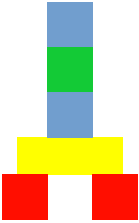
\includegraphics[scale=0.20]{figures/chapter2/task_goal.pdf}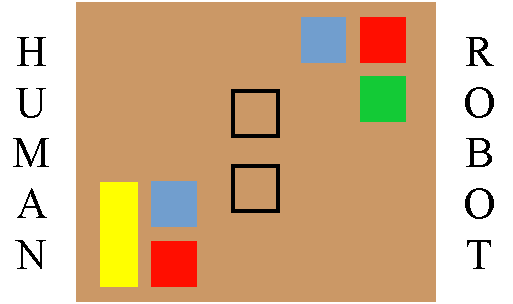
\includegraphics[scale=0.18]{figures/chapter2/task_setup_mini.pdf}}   
	\fancyhead[RO]{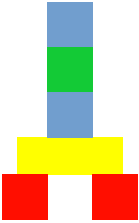
\includegraphics[scale=0.20]{figures/chapter2/task_goal.pdf}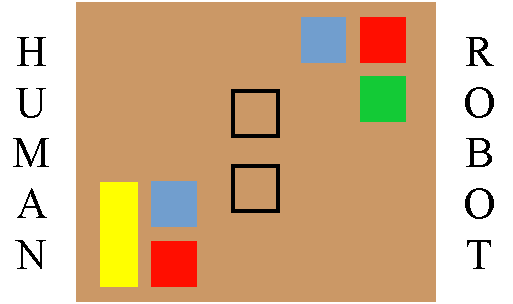
\includegraphics[scale=0.18]{figures/chapter2/task_setup_mini.pdf}\bfseries\thepage}  
	\fancyhead[RE]{\bfseries\nouppercase{\leftmark}}      % Chapter in the right on even pages
	\fancyhead[LO]{\bfseries\nouppercase{\rightmark}}     % Section in the left on odd pages
}%

\usepackage{pdfpages}
\usepackage{makecell}
\usepackage{pdflscape} 
\usepackage{mathtools}
\usepackage[section]{placeins}
\usepackage{afterpage}

%%%%%%%% my commands
\newcommand{\etal}{\textit{et al}.}
\newcommand{\ie}{\textit{i.e.}, }
\newcommand{\eg}{\textit{e.g.}, }
\newcommand{\fact}[3]{\mbox{\textit{#1}(#2, #3)}}
\newcommand{\circledtext}[1]{\raisebox{.5pt}{\textcircled{\raisebox{-.9pt} {#1}}}}
\newcommand{\sparql}{\textsc{SPARQL}}

\newcommand{\algConst}[1]{${\scriptscriptstyle #1}$}
\newcommand{\algNormTextSub}[2]{$\text{#1}_{#2}$}

\newcommand{\aslnumber}[1]{$#1$}
\newcommand{\aslstring}[1]{\textsf{#1}}
\newcommand{\aslvar}[1]{\textcolor{purple}{\textit{#1}}}
\newcommand{\asllabel}[1]{\textbf{#1}}
\newcommand{\annotation}[1]{{\footnotesize #1}}
\newcommand{\rulebody}[1]{\mbox{\hspace{.05\linewidth}}\begin{minipage}[t]{0.9\linewidth}#1.\end{minipage}}
\newcommand{\context}[1]{\begin{minipage}[t]{0.9\linewidth}#1\end{minipage}}
\newcommand{\planbody}[1]{\begin{minipage}[t]{0.9\linewidth}#1.\end{minipage}}
\newcommand{\Jason}[0]{\textbf{\textit{Jason}}}
\newcommand{\sn}{\mbox{\large\textbf{\texttt{\textasciitilde}}}}


\sloppy
\begin{document}
	\setcounter{chapter}{0} %% Numéro du chapitre précédent ;)
	\dominitoc
	\faketableofcontents
	\fi


\chapter{Lessons from Human-Human models}
\label{chapter:chap1}
\minitoc

This first chapter aims at setting the context for this thesis. First, we present some related works on human-human and human-robot social interactions. These works nourished the thoughts which led to this work. Then, we develop key elements for collaboration such as joint action, commitment and shared plans. Finally, we explore \acrfull{bdi} and cognitive robotic architectures  which have inspired us to design our own architecture in which, \acrshort{jahrvis} —  the main contribution of this thesis — endows a robot with the abilities not only to control, but also to evaluate its joint action with a human. 


\section{What is a social interaction?}
\label{chap1:sec:soc_int}

\subsection{How to define a social interaction?}
First, let’s take a look at the dictionary and see how the word \emph{interaction} is defined. According to the Oxford dictionary, an interaction is a ``reciprocal action or influence'' and more precisely a ``communication or direct involvement with someone or something''. As for the Cambridge dictionary, it defines it as an occasion when two or more people or things communicate with or react to each other''. Those definitions can give an hint about what it an interaction between humans but they are not specific enough. Now, going through social psychology literature, one of the first attempt to define \emph{social interaction} was by Goffman~\cite{goffman_1967_interaction}. He distinguished three basic interaction units: the social occasion, the gathering and the social situation. The social occasion is an event that is temporally and spatially situated in such a way that it forms a unit that can be looked forward and back upon, by participants that are informed by the event (dinner, meeting, sport game...). The gathering refers to any set of two or more individuals who are at the moment in one another’s immediate presence. It can be noted that a social occasion may include several gatherings but that gathering do not need social occasions to occur (they can happen in office spaces, street corners, restaurants…). The social situation refers to the full spatial environment that embraces interacting people. It is created as soon as people engage in interaction, when mutual monitoring occurs and ends when the next to the last person leaves. Furthermore, Goffman distinguished between focused and unfocused interaction (gathering). A focused gathering has its members that can come together to sustain a joint focus of visual and cognitive attention and are open to each other for talk. He calls it encounters or engagements. On the other hand, an unfocused gathering has its members present to one another but not engaged together (\eg persons waiting for a bus). In this same book, Goffman proposed a definition of social encounter: ``an occasion of face-to-face interaction, beginning when individuals recognize that they have moved into one another’s immediate presence and ending by an appreciated withdrawal from mutual participation''.

A couple of years later, Argyle wrote a book entitled Social Interaction~\cite{argyle_1973_social}, where he laid the foundations to understand social interactions. He came to the view that social interaction could be interpreted as a set of social skills, and that it may therefore be possible to train these skills the same way as manual skills are trained. For example, during an encounter between two persons, each must be able to perceive the social cues (verbal or non-verbal signals) of the other which are then filtered through the perspective each has acquired through socialization and experience.  The interpretation of context and social cues is then applied to come to a definition of the situation, which in turn guides both behavior and action.

Then, Rummel proposed a definition of a few words: ``Social interactions are the acts, actions, or practices of two or more people mutually oriented towards each other's selves, that is, any behavior that tries to affect or take account of each other's subjective experiences or intentions.''~\cite{rummel_1976_understanding}.

The elements brought here, trying to define what is an interaction and more precisely a social interaction, are chosen among a large amount of work. It is possible to find different definitions.

\subsection{Structure of a social interaction}\label{chap1:subsec:social_int}
Most of the research about interaction and social interaction belongs to the field of social psychology. As for the structure of a social interaction, it is more from the field of Conversation Analysis (CA) which mixes sociology, anthropology, linguistics, speech-communication and psychology.

Robinson makes a review of the work that has been done about \emph{overall structural organization}~\cite{robinson_overall_2012}. Most of the time in the literature, overall structural organization is discussed in terms of ``the overall structural organization of entire, single occasions of interaction''. Then, the \emph{overall structural organization} term is generally used to talk about one particular (albeit large) unit of interaction. However, many different types of interactional units can have an overall structural organization. For example, Schegloff encouraged to recognize ``‘overall structural organization’ not as something for the unit ‘a single conversation’ (or encounter, or session, etc.) alone, but for units like turns, actions and courses of action (like answering or telling), sequences, and who knows what else as well''~\cite{schegloff_2011_word}. He also mentioned that every unit of organization should probably have a local organization and a global organization. Here, the term \emph{overall structural organization} refers to ``the overall structural organization of entire, single occasions of interaction''. 

Robinson tells us that this concept has received relatively little analytic attention and thus is still not well understood~\cite{robinson_overall_2012}. Indeed, research has been more focused on analyzing the organization of individual sequences of action such as turn-takings or conversation openings. Several terms have been used to talk about a \emph{supra-sequential coherence}: big package, set of pre-organized sequences, (social) activity, project of activity or plan of action. Sacks gave the following definition for the overall structural organization of single occasions of interaction: it ``deals, roughly, with beginnings and endings, and how beginnings work to get from beginnings to something else, and how, from something else, endings are gotten to. And also the relationship - if there is one - between beginnings and endings''~\cite[p.~157]{sacks_lectures_1995}. Robinson summarized research about the subject by saying that single occasions of interaction (in a generic or context-free sense) are normatively organized as: (1) beginning with an opening (2) ending with a closing and (3) having ``something'' in between opening and closing'' which can be referred to as topics~\cite{robinson_overall_2012}.

\subsubsection{Opening}
Openings are used to begin an encounter. One of the main reference on the subject is the work of Schegloff~\cite{schegloff_1986_routine}. Openings and related issues vary depending on the nature of interactions. For example, opening of a phone call to a family member or a friend will be organized as follow: (1) summons-answer (the one calling talks first) (2) identification/recognition of each other (3) greetings and (4) how-are-you. Whereas, in primary-care medical visits, opening is sequenced as: (1) greeting (2) securing patients’ identities (2) retrieving and reviewing patients’ records and (4) embodying readiness (sitting down and facing one another). More examples from the literature can be found in (Robinson, 2012). 

Another work, by Kendon~\cite{kendon_1990_conducting}, focuses on the greeting part, but more precisely the greeting behavior with the associated non-verbal cues. The greeting behavior is divided in three main phases: the distance salutation, the approach and the close salutation. 
The distance salutation only occurs if the greeters as far enough such as they need to get closer if they wish to continue the interaction. This phase starts after one or both participants sight one another and at least one of them identifies a wish to engage in a greeting. In case one of the participant has not seen the other one, he signals his presence by vocalizing the other one’s name or by clearing his throat. Then, they orient their bodies towards each other and exchange glances in a subtle acknowledgement that the greeting is desired by both. During this phase, people can also wave or give a sign with their head (\eg nod).
The approach is divided into two sub-phases: the distant approach and the final approach. During the distant approach, people tend to look away whereas when the final approach starts (the greeters are 3 meters or less from one another), they look back at each other and, they smile.
Finally, there is the close salutation, the most normalized phase of the greeting. It happens when people are 1,5 meters or less from each others. Then, they can have a non-contact close salutation during which people exchange verbal greetings, or they can hand-shake or embrace (or do something else according to their culture). The greeting is over.

\subsubsection{Topics}
Episodes of interaction vary a lot in their contextualized nature, which leads to a large variety of topics and sequences of topics. Interactions that happen in ordinary or institutional contexts can be pre-organized around one or more topics. Robinson gave examples such as an emergency call or an expected call back by a friend to discuss an expected single item of business~\cite{robinson_overall_2012}.

\subsubsection{Closing}
Schegloff is one of the reference on closing as well~\cite{schegloff_1973_opening}. A closing can be divided into two phases: the topic termination and the leave-taking.
The topic termination has a pre-closing statement which signals to the partner the wish to close the conversation. Then, the leave-taking follows the pre-closing statement and its response and, includes the goodbye exchange. Finally, the partners break co-presence, \ie physically walk apart.\footnote{It is not explicitly mentioned in~\cite{schegloff_1973_opening}  but they precise in a footnote that it would not make sense if the parties remain in co-presence after having being through the closing sequence.} In the context of a phone call, Clark and French defined this co-presence breaking as the \emph{contact termination} when people hang up~\cite{clark_1981_telephone}.

With regards to non-verbal cues, Knapp \etal{} listed and analyzed them~\cite{knapp_1973_rhetoric}. The more frequent are eye contact breaking, head nodding, leaning toward the partner and positioning in the direction of the way of leaving.

\section{How do we represent the ``other''? -- Theory of Mind}~\label{chap1:subsec:tom}
%\subsection{Theory of Mind}~\label{chap1:subsec:tom}
\acrfull{tom} refers to the ability to represent others' intentions, beliefs, knowledge, goals, \ie their \emph{unobservable mental states}~\cite{premack_1978_does,povinelli_2004_we}. Thus, this concept is related to some presented above. Indeed, common knowledge requires \acrshort{tom} as ``to know what another knows and to be capable of making the sorts of inferences required for common knowledge, one must have an understanding of others (or an understanding of a particular person) in terms of thoughts and beliefs''~\cite[p.~82]{tollefsen_2005_let}. And thus, shared intention, as stated by Pacherie, ``having a shared intention typically presupposes cognitively and conceptually demanding theory of mind skills''~\cite[p.~1817]{pacherie_2013_intentional}. Moreover, some authors showed that \acrshort{tom} development and functioning relied on joint attention~\cite{sodian_2015_declarative, camaioni_2004_role}.  Finally, it has been shown that \acrshort{tom} improves joint planning and so increases the ability to cooperate in joint activity~\cite{astington_1995_theory}. We can note that Westby and Robinson explained that recent research about \acrshort{tom}, showed that \acrshort{tom} is not only to understand what others think, know, believe or intend (cognitive \acrshort{tom}) but that another part of \acrshort{tom} involves thinking about and experiencing the emotions of others (affective \acrshort{tom})~\cite{westby_2014_developmental}. In this manuscript, we will leave aside the latter.

As for common knowledge (see Section~\ref{chap1:subsubsec:common_g}), there is an infinite number of levels, or orders to \acrshort{tom}. Most often, the focus is on the first and the second orders. Perner and Wimmer defined the ``first-order belief attribution'' as the estimation of one's beliefs (\eg I think she thinks that) and the ``second-order belief attribution'' as the estimation of what one  thinks about what another person is thinking or feeling (\eg I think she thinks I think that)~\cite{perner_1985_john}. Based on the same principle, Flavell \etal{} proposed levels of role-taking where the Level 1 is defined as ``S thinks (knows, predicts or whatever) that O has such-and-such belief (attitude, feeling, etc.) about something (X), about S himself, about O himself or about some other individual or group (O\textsubscript{1})'' (\eg ``I know how you feel (about something or someone)''). The level 2 is defined as ``S thinks that O is aware of (unaware of, dislikes, etc.) S's or O\textsubscript{1}'s thoughts (feelings, perceptions, etc.) regarding X, S, O or O\textsubscript{1}'' (\eg ``I'm sure you know what I think about Bill'')~\cite[pp.~49--51]{flavell_1968_development}.

\paragraph{And perceptive-taking} \acrshort{tom} is also closely related to another notion that we have not mentioned yet but that is of interest in \acrshort{hri}: perspective-taking, which is mostly studied in psychology, sociology and neurology. These fields study how people understand each others and refer to it in different ways: social perspective-taking or role-taking, perspective-taking or empathy~\cite{davis_2017_self,quesque_2020_theory}. Sometimes, \acrshort{tom} and perspective-taking are used interchangeably, as by Charlop-Christy and Daneshvar defining perspective-taking as an elementary aspect of \acrshort{tom}~\cite{charlop_2003_using} or \acrshort{tom} can be a synonym of ``cognitive perspective-taking''~\cite{barnes_2004_perspective}. 

While, some authors, like Westby and Robinson, differentiated them and showed that perspective-taking is an element among others of \acrshort{tom}~\cite{westby_2014_developmental}. Actually, the perspective-taking to which they referred is the one \emph{called visual perspective-taking} which is a type of \emph{perceptual perspective-taking}. Indeed, perspective-taking, as \acrshort{tom} has several dimensions. Some authors distinguish between \emph{perceptual perspective-taking}, referring to the inference that a person makes regarding another person's visual, auditory, or other perceptual experience; and \emph{conceptual perspective-taking}, referring to the inference that one makes regarding another's internal experience such as his thoughts, desires, attitudes, plans~\cite{marvin_1976_early}. 

Others distinguish two different dimensions: ``\emph{cognitive perspective-taking} may be defined as the ability to infer the thoughts or beliefs of another agent, while \emph{affective perspective-taking} [or emotional~\cite{hynes_2006_differential}] may be defined as the ability to infer the emotions or feelings of another agent''~\cite{healey_2018_cognitive}. According to the task, they can be requirements for \acrshort{tom}~\cite{hynes_2006_differential}. Cognitive perspective-taking is central to communication, particularly in the creation and understanding of referring expression (\ie a word or phrase to identify an object)~\cite{krauss_1991_perspective}.

\bigskip

Another element of \acrshort{tom} that we will discuss here is the ability to attribute false belief to others, \ie make the distinction between the reality and what one can believe about the world~\cite{dennett_1978_brainstorms}, as tasks demonstrating this ability have been extensively used to test theory of mind of individuals, such as the task created by Wimmer and Perner~\cite{wimmer_1983_beliefs} and then extended by Baron-Cohen \etal{} which is the most famous false belief task, the Sally--Anne test~\cite{wimmer_1983_beliefs, baron_1985_does}. In the experiment, children are presented two characters, Sally (who has a basket) and Anne (who has a box). Then, Sally departs, leaving a object A in her basket. While Sally is away, Anne removes the object and hides it in her box. Children are asked to predict, on Sally's return to the room, where Sally will look for the object. Authors used to claim that children being able to answer to this question had \acrshort{tom} whereas others did not. Nowadays, it has been shown that false belief tasks are not enough to assess \acrshort{tom}~\cite{bloom_2000_two, wellman_2001_meta}.

\section{What is a joint action?}\label{chap1:sec:ja}
%\section{Around the Joint Action Concept}\label{chap1:sec:ja}
Often, multiple concepts are addressed when referring to collaborative tasks: collaboration, cooperation, coordination, joint action, joint activity, shared/joint attention, shared/joint intention, shared plan, shared/common/joint goal, (joint) commitment, engagement, mental states, theory of mind, mutual knowledge... However, many terms and definitions, whether inside a field\footnote{Here, philosophy, psychology or robotics} or between fields do not reach a consensus. This can be quite confusing, especially for roboticists for which it is initially not the range of expertise. Thus, we will first give an overview of the more characteristic definitions of what is Joint Action. Then, we will present a non-exhaustive set of notions related to Joint Action. 

A part of this work on Joint Action, realized in the context of the JointAction4HRI project\footnote{https://jointaction4hri.laas.fr/}, is the result of the collaborative work with Kathleen Belhassein, a PhD student in psychology, and V{\'\i}ctor Fern{\'a}ndez Castro, a post-doctoral researcher in philosophy. It has been the subject of a publication in the book Culturally Sustainable Social Robotics~\cite{belhassein_2020_horizontal} with a focus on communication, a publication under submission at Acta Psychologica~\cite{belhassein_2021_adressing} discussing joint action in \acrshort{hri} and a publication under submission in a volume of the Book Serie Techno:Phil~\cite{castro_2021_adressing} tackling commitments in \acrshort{hri}.

\subsection{How to define Joint Action?}\label{chap1:subsec:def_ja}

An important number of social interactions and encounters are encompassed by the notion of joint action. Broadly considered, joint action is any form of social interaction whereby two agents or more coordinate their actions in order to pursue a joint goal. However, the notion of joint action has particularly been subject to debate in philosophy and psychology. For instance, according to Sebanz \etal~\cite[p.~70]{sebanz_2006_joint}, ``joint action can be regarded as
any form of social interaction whereby two or more individuals coordinate their actions in space and time to bring about a change in the environment.''; while other authors~\cite{carpenter_2009_just, cohen_1991_teamwork, fiebich_2013_joint, tomasello_2005_understanding,pacherie_2012_agency} resist the idea that instances of mere coordination – \eg two partners walking side by side – constitute a joint action, considering that it requires some necessary conditions like sharing goals and intentions.

Moreover, while the notion of joint action is used interchangeably with the notion of \emph{collaboration} or \emph{cooperation} for some authors such as Becchio \etal~\cite{becchio_2010_toward} and Kobayashi \etal~\cite{kobayashi_2018_language}, other authors establish a hierarchy of interactions depending on the processes involved~\cite{amici_2015_coordination, chalmeau_1995_cooperation}. According to Amici and Bietti, for example, coordination is a fast low-level process of behavioral matching and interactional synchrony which could, but not necessarily, facilitate middle-level processes like cooperation, collaboration or high-level processes like joint action, which requires other resources like turn-taking and alignment of linguistic resources during dialogue. ``To date, however, little is known about the exact way in which coordination, collaboration and cooperation are linked to each other''~\cite[p.~vii]{amici_2015_coordination}. Looking at the APA dictionary, collaboration is ``the act or process of two or more people working together to obtain an outcome desired by all, as in collaborative care and collaborative learning'' and ``cooperation a process whereby two or more individuals work together toward the attainment of a mutual goal
or complementary goals. [...] Often cooperation leads to outcomes [...] but the benefit to each individual is not always obvious''~\cite{sharbrough_2015_apa}. Thus, here the nuance is in the process benefit and not in the temporal level.

If we look at Sebanz and colleagues definition of joint action, it could be considered as a kind of activity (based on the usual sense of the term activity). Thus, some authors use the concept \emph{joint activity} interchangeably with \emph{joint action}~\cite{tollefsen_2005_let,grafenhain_2013_three} while others see the joint activity composed of joint actions~\cite{clark_1996_using, feltovitch_2005_common}. Clark says that ``joint activities advance mostly through joint actions''~\cite[p~.59]{clark_1996_using}. He defines the properties of a joint activity among which there are: it is carried out by 2 or more participants, each participant has a public role or they try to establish and achieve joint goals, and they may have private goals. He also highlights the need for coordination: ``What makes an action a joint one, ultimately, is the coordination of individual actions by two or more people. There is coordination of both \emph{content}, what the participants intend to do, and \emph{processes}, the physical and mental systems they recruit in carrying out those intentions''~\cite[p~.59]{clark_1996_using}. 

Sometimes, it is also possible to come across \emph{collaborative activity}~\cite{tomasello_2005_understanding}, \emph{collaborative task}~\cite{brennan_2008_coordinating} or \emph{collaborative joint action}~\cite{godman_2013_we} (less frequent). Tomasello \etal{} claimed that ``collaborative activities require both an alignment of self with other in order to form the shared goal, and also a differentiation of self from other in order to understand and coordinate the differing but complementary roles in the joint intention''~\cite[p.~681]{tomasello_2005_understanding}. Carpenter, one of the author of this latter article, uses the terms \emph{collaborative activity} and \emph{joint activity} to refer to the same task but giving a social dimension to collaborative activity, being ``an end in itself rather than just a means of getting something done''~\cite[p.~384]{carpenter_2009_just}. For Pacherie, joint actions are performed by the partners in order to achieve the joint goal of a collaborative activity or joint activity~\cite{pacherie_2013_intentional}.

As we can see, it is not possible to propose a unified definition of these terms based on the literature. In this manuscript, the word joint action will be used to indifferently refer to an activity/task composed of several (joint) actions, \ie a high level joint action or as a single action, but in both cases it will imply that it is a ``social interaction where two or more individuals coordinate their actions in pursuit of a common goal''~\cite{castro_2020_joint}. We will also use \textit{joint activity} to refer to high level joint actions. Moreover, \acrshort{hri} often refers to collaborative tasks when the robot and the human perform an activity together, thus, we will also use this term which we consider as involving joint actions.

\subsection{Two possible segmentations around Joint Action}

Before going through the mechanisms involved in joint action, we will briefly present two segmentations of joint action: a temporal segmentation, \ie the different phases a joint action goes through, and a cognitive model for human agency \ie the different neurocognitive levels that are involved in joint action. It seemed necessary to present these two segmentations as the processes related to joint action described in Section~\ref{chap1:subsec:necess_ja} are sometimes involved in one phase/level but not in another. However, we will not go through these details as it is not necessarily relevant to the rest of the manuscript.

\subsubsection{Temporal segmentation of Joint Action}
As a joint action is a form of social interaction, it can also be divided in three phases as presented in Section~\ref{chap1:subsec:social_int}: an initiation, a body and a closing~\cite{heesen_2017_social}. Each phase has a role. First, the initial phase establishes among other things the joint commitment, \ie who is to participate, in what roles (these can vary during the interaction), what actions are they performed, and when and where they will be performed~\cite{clark_2006_social}. Then, in the body participants coordinate to perform their goal. Finally, ``to complete a joint action, participants first need to arrive at the mutual conviction that they are both indeed ready to terminate it''~\cite{heesen_2017_social}, if they achieved their goal for example.

At a lower level of joint action, the level of action and not social interaction, joint action can be seen as a process with two phases: planning and execution. Curioni \etal{} proposed a model, specifying what happens in each phase~\cite{curioni_2017_joint}: 
\begin{bulletList}
	\item planning: 
	\begin{bulletList}
		\item expectations on partner's intentionality
		\item selecting action possibilities
		\item establishing commitment
	\end{bulletList}
	\item execution:
	\begin{bulletList}
		\item aligning attention to objects and events
		\item maintaining commitment
	\end{bulletList}
\end{bulletList}
\subsubsection{Neurocognitive segmentation of Joint Action}~\label{chap1:subsubsec:neuro_seg}

To describe the levels of the neurocognitive mechanisms involved in joint action, we will base ourselves on the conceptual framework of action established by Pacherie~\cite{pacherie_2008_phenomenology}. This framework is particularly relevant for the rest of manuscript as it has a lot similarities with the three-layered robotic architecture that will be described in Section~\ref{chap3:sec:rob_archi}, as noticed in~\cite{clodic_2017_key}. It is based on a dynamic model of intentions and distinguishes:

\begin{bulletList}
	\item A distal intentions level (D-intentions) in charge of the dynamics of decision making, temporal flexibility and high level rational guidance and monitoring of action;
	\item A proximal intentions level (P-intentions) that inherits a plan from the previous level and whose role is to anchor this plan in the situation of action, this anchoring has to be performed at two levels: temporal anchoring and situational anchoring;
	\item A motor intentions level (M-intentions) -- which encodes the fine-grained details of the action (corresponding to what neuroscientists call motor representations) -- is responsible for the precision and smoothness of action execution, and operates at a finer time scale than either D-intentions or P-intentions
\end{bulletList}

This model of action has then been enriched with the specificities of joint action in~\cite{pacherie_2012_agency}, integrating at each levels the representations and processes associated to the joint action partner. We will not go through the details of it here but they will be mentioned all along Section~\ref{chap1:subsec:necess_ja}.

\subsection{What is necessary for Joint Action?}\label{chap1:subsec:necess_ja}

Leaving aside the debate on the concept of joint action, we aim to focus on the mechanisms that enable the consecution of joint actions. What we found to be the mechanism on which every author (or almost) agrees on to say that it is required for a joint action is the \emph{coordination}. This mechanism itself is supported by other cognitive and sensorimotor processes. Also, philosophers introduced another concept involved in joint action which is the \emph{shared intention}. In Figure~\ref{chap1:fig:ja}, we made an attempt to represent, in a non-exhaustive way, a number of these processes and how they are connected to each other, based on our analysis of the concepts involved.

\begin{figure}[!ht]
	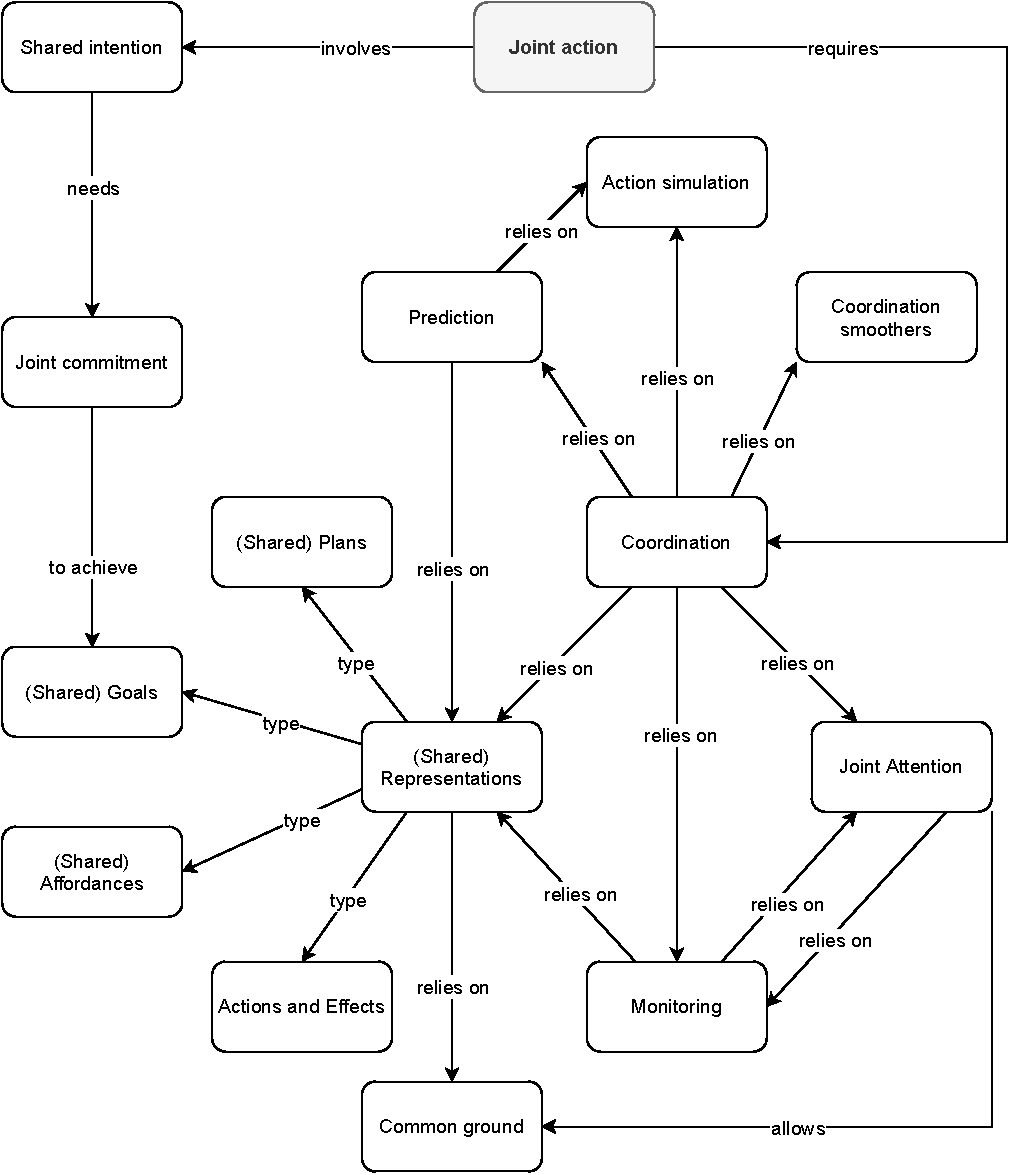
\includegraphics[width=\linewidth]{figures/chapter1/joint_action.pdf}
	\caption{Mapping of a non-exhaustive set of processes related to joint action}
	\label{chap1:fig:ja}
\end{figure}

We will first present the concepts of \emph{shared intention} and \emph{joint commitment} and then define the concept of \emph{coordination} and its associated mechanisms. 

\subsubsection{Shared Intention}
First, before coming to the concept of shared intention, what is an intention? We are going to take a look at three definitions, first from a philosopher (Bratman), then from computer scientists (Cohen and Levesque) and finally from psychologists (Tomasello \etal). 

Sometimes, we talk about intention to refer to something we do intentionally (action) or to refer to things we intend to do (mental state). Thus, Bratman distinguishes both~\cite{bratman_1984_two} associating the first possibility to what he calls present-directed intention (I may intend to start my car now) and the latter to future-directed intention (I may intend to start my car later today). But, ``when I am starting my car it may seem natural to say that I no longer intend to start it, I am starting it''~\cite[p.~379]{bratman_1984_two}. He chose to concentrate on future-directed intentions rather than present-directed intentions when referring to intentions. 

Cohen and Levesque based their definition of intention on this view of Bratman~\cite{cohen_1990_intention}. They added the notions of commitment and goal: ``An intention is defined as a commitment to act in a certain mental state: An agent intends relative to some conditions to do an action just in case she has a persistent goal (relative to that condition) of having done the action, and, moreover, having done it, believing throughout that she is doing it''~\cite[p.~496]{cohen_1991_teamwork}. 

The definition of Tomasello \etal{} includes the notion of plan since they defined an intention as ``a plan of action the organism chooses and commits itself to in pursuit of a \emph{goal}. An intention thus includes both a means (action \emph{plan}) as well as a goal''~\cite[p.~676]{tomasello_2005_understanding}. 

Now that we have a clearer idea of an intention, we can focus on shared intention. We will start again with Bratman~\cite{bratman_1993_shared}. He considers that two agents have the shared intention to J if and only if: 
\begin{enumerate}
	\item (a) [agent X] intend that [they] J and (b) [agent Y] intend that [they] J.
	\item\relax [agent X] intend that [they] J in accordance with and because of 1a, 1b, and meshing subplans of 1a and 1b; [agent Y] intend that [they] J in accordance with and because of 1a, 1b, and meshing subplans of 1a and 1b.
	\item 1 and 2 are \emph{common knowledge} between [them].
\end{enumerate}

Tomasello, \etal{}, them, use the terms shared intentionality (``we'' intentionality) and joint intention~\cite{tomasello_2005_understanding}. For them, ``shared intentionality [...] refers to collaborative interactions in which participants have a \emph{shared goal} (\emph{shared commitment}) and coordinated action roles for pursuing that shared goal''. They based this definition on the works of Gilbert~\cite{gilbert_1989_social}, Searle~\cite{searle_1983_intentionality} and Tuomela~\cite{tuomela_1995_importance}. They defined joint intention as a form of shared intentionality where each partner's ``representation of the intention [...] contains both self and other'', as we can see in their illustration, reproduced in Figure~\ref{chap1:fig:ji}. We can also find other close terms such as Bratman who referred to Searle and Tuomela about their definition of ``we-intention'', highlighting the difference with shared intention. He explained that ``we-intentions'', also called ``collective intentions'' are intention of an individual concerning a group's or collective's activity, and there can be such intention even though there is only one individual (falsely believing others are involved)~\cite{bratman_1993_shared}. Whereas, a shared intention necessarily involved at least two persons. Thus, it can be compared with Tomasello \etal{}'s definition of joint intention. Some authors such as Tollefsen use joint intention and shared intention interchangeably~\cite{tollefsen_2005_let}.

 \begin{figure}[!ht]
 	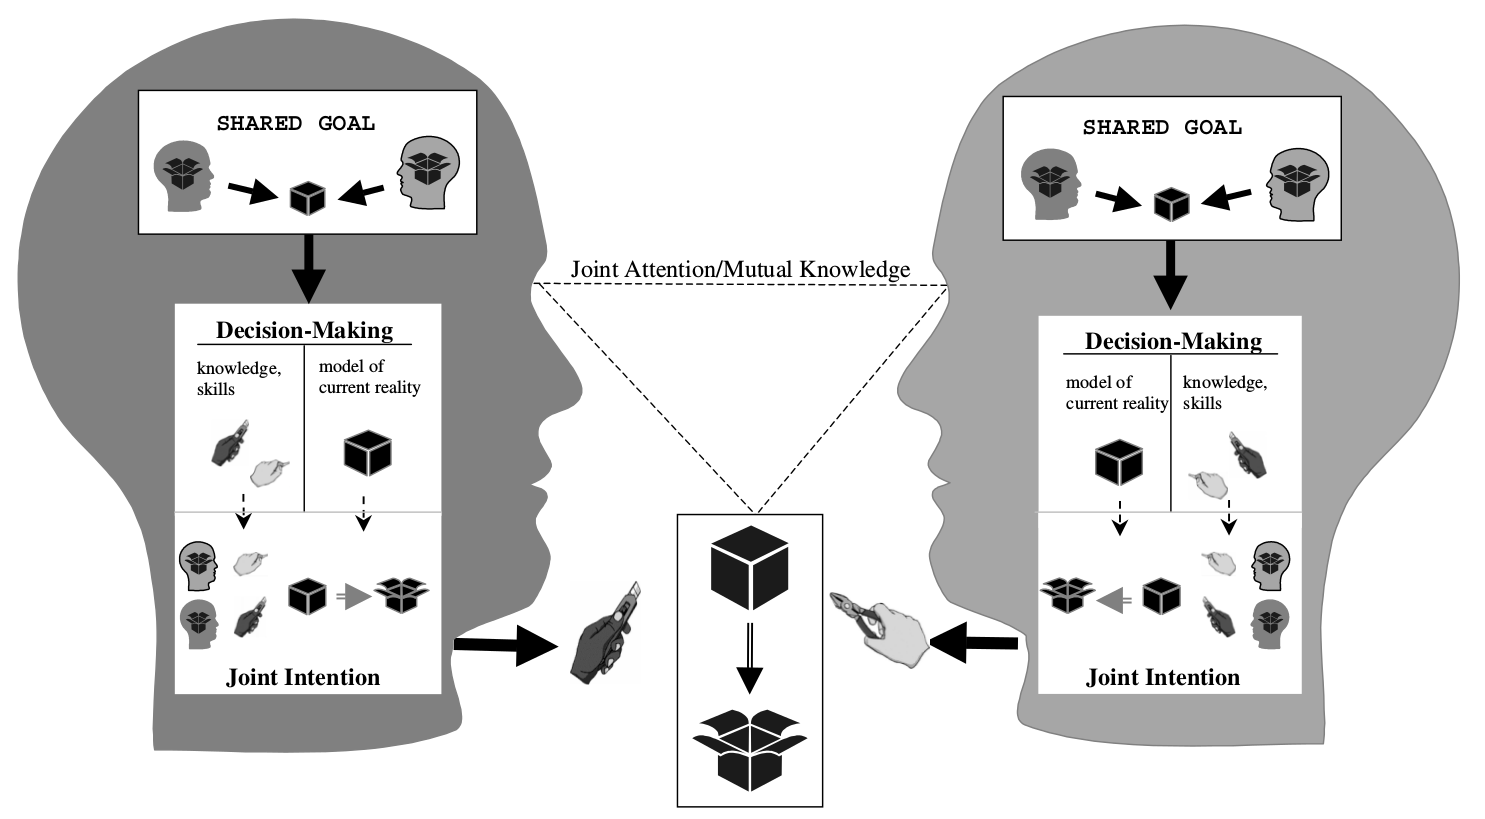
\includegraphics[width=\linewidth]{figures/chapter1/shared_representation.png}
 	\caption{Illustrative example of a collaborative activity by Tomasello \etal~\cite{tomasello_2005_understanding}. Here the humans have for shared goal to open the box together. They choose a means to perform it which takes into account the other's capabilities and so form a joint	intention.}
 	\label{chap1:fig:ji}
 \end{figure}

Cohen and Levesque took their inspiration from Bratman's definition of shared intention in their view of joint intention for artificial agents, considering joint intention as a future-directed \emph{joint commitment} to perform a collective action while in a joint (or shared) mental state.

\subsubsection{Joint Commitment}\label{chap1:subsubsec:joint_commit}
Commitments can be understood as ``a triadic relation among two agents and an action, where one of the agents is obligated to perform the action as a result of having given an assurance to the other agent that she would do so, and of the other agent’s having acknowledged that assurance under conditions of common knowledge''~\cite[p.~756]{michael_2017_commitment}. Commitments are not necessarily established through promises or even explicit verbal communication~\cite{ledyard_1994_public, scanlon_2000_we, siposova_2018_communicative}, however, this basic definition allows us to see the fundamental component of a commitment. But why are commitments important for joint action?

In philosophy and psychology, many authors have emphasized the importance of commitments for joint action such as Cohen and Levesque~\cite{cohen_1991_teamwork}, Clark~\cite{clark_2006_social}, Gilbert~\cite{gilbert_2009_shared}, Bratman~\cite{bratman_2014_shared}, Michael and Pacherie~\cite{michael_2015_commitments}, Roth~\cite{roth_2014_shared} or Siposova \etal~\cite{siposova_2018_communicative}. 

For instance, in philosophy, Gilbert~\cite{gilbert_2009_shared} and Bratman~\cite{bratman_2014_shared} have largely argued about the requirements for people to establish shared intentions and their role in explaining social coordination. While Bratman has argued that shared intentions can be understood as an aggregation of individual intentions which only requires individual commitments with general standards of rationality, Gilbert has argued that shared intentions are essentially tied to joint commitments. According to her, two or more persons share an intention to do something if and only if they are jointly committed to intend as a body to do it~\cite{gilbert_2009_shared}. In other words, joint actions require the people involved to impose obligations to each other. Further, Roth has argued that joint action requires the participants to be committed to the activity in the Gilbert’s sense, which also implies contralateral commitments that hold across the other participants in the shared activity~\cite{roth_2014_shared}. For instance, if Sue and Jack agree on going for a walk together, they share a commitment to carry out the shared action but also, they assume an individual contralateral commitment to keep pace with each other. In brief, commitments are essential for the establishment of joint and individual intentions during shared activities. 

In psychology, several authors, such as Clark~\cite{clark_2006_social}, Michael \etal~\cite{michael2016} or Siposova \etal~\cite{siposova_2018_communicative}, have studied how implicit and explicit communication are used to establish commitments and their importance for coordinated actions. For example, Clark has emphasized how partners use communicative exchanges like projective pairs, where one of the participants proposes a particular goal to another (Let’s do G! Should we do that?), who then accepts or rejects the proposal~\cite{clark_2006_social}. Those exchanges are pervasive in human-human coordinated actions and they serve to negotiate goals, plans and social roles which are translated into an amalgamate of different types of commitments that are necessary for the execution of the general \emph{joint goal}. Michael \etal{} suggest that people often use investment of effort in a task as an implicit cue for making the perceiver aware that we expect him to behave collaboratively which often triggers a sense of commitment that motivates actions~\cite{michael2016}. Furthermore, Siposova \etal{} have found that humans use implicit cues like gaze signals to communicate an agreement or commitment to carry out a task their partner intends to perform~\cite{siposova_2018_communicative}.

To summarize about joint commitment, we retain the words of Gilbert~\cite[p.~7]{gilbert_2013_joint}: ``a joint commitment is a commitment of the two or more people involved. It is, more fully, a commitment by two or more people of the same two or more people'', keeping in mind that it ``is not a concatenation of personal commitments''. 

\subsubsection{Coordination}
Coordination is a central mechanism to distinguish individual actions from joint actions. There has been an important deal of conceptual and empirical work investigating this process, such as the one of Knoblich \etal~\cite{knoblich_2011_joint} and the one of Pacherie~\cite{pacherie_2012_agency}. Coordination relies on several mechanisms. They can be non-intentional -- sometimes called emergent coordination~\cite{knoblich_2011_joint} -- such as perception-action matching~\cite{brass_2001_movement}, perception of joint affordances~\cite{ramenzoni_2008_short} or action simulation~\cite{sebanz_2009_prediction}. As for intentional coordination – sometimes referred to as planned coordination~\cite{knoblich_2011_joint} –, it requires the partners: (i) to represent their own and others' actions, as well as the consequences of these actions, (ii) to represent the hierarchy of sub-goals and sub-tasks of the plan, (iii) to generate predictions of their joint actions, and (iv) to monitor the progress toward the joint goal in order to possibly compensate or help others to achieve their contributions~\cite{pacherie_2012_agency}. From Section~\ref{chap1:subsubsec:shared_rep} to Section~\ref{chap1:subsubsec:coord_smooth}, we present a non-exhaustive set of joint action mechanisms on which relies coordination. We chose the ones that seemed: to be the most mentioned in the philosophy and psychology literatures, to obtain consensus about their involvement in coordination and to be relevant to Human-Robot Interaction. 

\subsubsection{(Shared) Representations}\label{chap1:subsubsec:shared_rep}
As stated by Sebanz \etal, joint action depends on the ability to share representations~\cite{sebanz_2006_joint}. Representation sharing is present at different levels, \ie agents can share representations of objects, events, actions, goals, plans and tasks~\cite{pacherie_2012_agency,vesper_2017_joint}. These representations enable, among other things, the prediction (see Section~\ref{chap1:subsubsec:pred}) of other's actions. 

\paragraph{Representation of (Shared) Tasks}
A task can be described at multiple grains or levels of abstraction~\cite{cooper_2000_contention},  the same action can be described
as both ‘putting a piece of toast in one’s mouth’ and ‘maintaining an adequate supply of nutrients’. A used definition in psychology is that ``a task consists of producing an appropriate action (\eg conveying to mouth) in response to a stimulus (\eg toast in a particular context)''~\cite[p.~1]{monsell_2003_task}. Sebanz \etal{} extended this definition with the possibility to execute more than one action when responding to a stimulus~\cite{sebanz_2005_two}. 

How to share a task? Sebanz \etal{} proposed that ``sharing a task representation or corepresenting a task then means that an individual represents at least one rule that states the stimulus conditions under which a coactor should perform a certain action''~\cite[p.~1235]{sebanz_2005_two}.
In another paper, in the context of joint action, Sebanz \etal{} evoked studies showing the formation of shared representations during collaborative tasks, \ie an agent knows what the other should do and represents it in a functionally equivalent way to their's own. They concluded that it allowed individuals ``to extend the temporal horizon of their action planning,
acting in anticipation of others’ actions rather than simply responding''~\cite[p.~73]{sebanz_2006_joint}.


\paragraph{Representation of (Shared) Goals}
Goal has two meanings leading sometimes to ambiguities: the state-to-reach of the environment (external goal) and the mental representation of a desired state (internal goal)~\cite{tomasello_2005_understanding}. It is interesting to be aware of this double meaning. 

Several authors highlighted the need of the representation of a shared goal for joint action such as Pacherie~\cite{pacherie_2012_agency}, Tomasello \etal{}~\cite{tomasello_2005_understanding} or Cohen and Levesque~\cite{cohen_1991_teamwork}. Sometimes they use the terms  common goal~\cite{searle_1990_collective}, joint goal or joint persistent goal.
Based on Braman~\cite{bratman_1992_coop}, Tomasello \etal{} affirmed that ``there is a shared goal in the sense that each participant has the goal that we (in mutual knowledge) do X together'' and that ``each interactant has goals with respect to the other’s goals''~\cite{tomasello_2005_understanding}. Pacherie listed as a condition for joint action that each agent has to represent their goals and their coagents goals~\cite{pacherie_2012_agency}.

\paragraph{Representation of (Shared) Plans}
A intention is sometimes defined as a plan of actions that an agent chooses to achieve a given goal~\cite{tomasello_2005_understanding, kaplan_2006_challenges}. 
As for shared goals, Tomasello \etal{} and Pacherie highlighted the need for an agent to represent ``their own subplans and the meshing parts of the subplans of others, and some of what they represent is to be performed by others''~\cite[p.~353]{pacherie_2012_agency}.

Representations, models of plans and shared plans are more studied by computer scientists than by philosophers and psychologists, proposing computational models such as the ones of Grosz and Kraus. They demonstrated that shared (collaborative) plans should not be treated as the sum of individual plans but as plans necessitating from the agents joint intentions, a mutual belief of how to perform the task and eventually individual or shared plans to perform the task's actions~\cite{grosz_1996_collaborative}.

\paragraph{Representation of Actions and Effects}
Studies showed that when an agent observes an action, a corresponding representation in their action system is activated~\cite{rizzolatti_2004_mirror}. Sebanz \etal{} affirmed that representation sharing is essential to joint action, specially action representations, as ``individuals could be ‘on the same page’ action-wise by sharing representations of actions and their underlying goals''~\cite[p.~71]{sebanz_2006_joint}. Pacherie evokes the need of agents to have the ability to have not only a representation of actions to be performed, self's and other's, but also their consequences~\cite{pacherie_2012_agency}. 

\paragraph{Affordances}
The concept of affordances has been introduced in 1966~\footnote{\url{https://www.merriam-webster.com/dictionary/affordance}} by Gibson, a psychologist, who presented his theory in~\cite{gibson_1979_theory}. He coined the term to refer to what the environment has to offer to the animal (individual), ``what it provides or furnishes, either for good or ill''. Then, the term and concept became popular and have been used in other fields than the original one (ecological psychology) such as cognitive psychology, human-computer interaction or design. Osborne discussed in his thesis~\cite{osborne_2014_ecological}, among other things, the history of the word and the different uses and meaning there are nowadays (see also two reviews on affordances~\cite{jamone_2016_affordances, bach_2014_affordance}). The definition that is commonly used in HCI/HRI has been introduced by Norman, a design researcher, in 1988 which claimed that ``affordance refers to the perceived and actual properties of the thing, primarily those fundamental properties that determine just how the thing could possibly be used''~\cite[p.~9]{norman_1988_psychology}. Thus, it became associated to the term \emph{action possibilities}. 

What about affordances when people are in a joint action? Richardson \etal{} showed that when acting together, people take into account not only their motor affordances but also the ones of their partners, helping to decide whether to perform a joint action or an individual action with an object~\cite{richardson_2007_judging}. Thus, Knoblich \etal{} called \emph{common affordance} ``when two agents have similar action repertoires and perceive the same object [will likely] engage in similar actions because the object affords the same action for both of them''~\cite[p.~63]{knoblich_2011_joint}, enabling coordination as agents perceive the same objects at the same time. They called \emph{joint affordance} when ``objects have an affordance for two or more people collectively [(a two-handled saw)] which is not necessarily an affordance for any of them individually''.


\subsubsection{Joint Attention}\label{chap1:subsubsec:joint_att}
We will start with two complementary definitions of \emph{attention}. The first one is from Tomasello \etal{} who say ``attention may thus be thought of as intentional perception (selective attention)''~\cite{tomasello_2005_understanding}. The second one is from Kaplan and Hafner~\cite{kaplan_2006_challenges} who define attention as ``the temporally-extended process whereby an agent concentrates on some features of the environment to the (relative) exclusion of others''. They distinguish two situations for which the process can occur: (1) passive attention when a salient event happens and thus automatically triggers the attention of the agent, and (2) active attention when the agent is involved in an
intentionally directed process and must actively select particular features of its environment. 

What happens to this process in the context of a joint action? We then talk about \emph{joint attention}. To perform a joint action, partners need a common goal. Indeed, joint action requires that individuals plan and perform their actions according to their predictions about the other’s actions to reach this goal. Joint attention is a key feature for this purpose, playing a crucial role in ``being and acting together''~\cite{tomasello_2009_cultural}, as it allows the partners to establish and share a perceptual common ground, necessary to initiate the joint action but also for individuals already engaged in a joint action to coordinate successfully. 

Despite this agreement to affirm that joint attention is important for joint action, Siposova stated that ``there is still surprisingly little agreement on exactly what joint attention is and how it is achieved''~\cite{siposova_2019_new}. While for some authors, two agents orienting their attention towards the same referent is a sufficient criterion to speak about joint attention~\cite{butterworth_1991_minds}, others like Pacherie precised that ``the phenomenon of joint attention involves more than just two people attending to the same object or event''. A classic way to define joint attention is the ability to coordinate our attention to the same object of interest (\eg as shown by Bakeman and Adamson~\cite{bakeman_1984_coordinating}), enabling us to integrate others’ attentional focus and therefore to experience the world together as described by Tomasello~\cite{tomasello_2009_cultural}.  ``The attentional focus of the two persons must be truly joint in the sense that both participants are \emph{monitoring} the other's attention to the outside entity''~\cite[p.~106]{tomasello_1995_joint}, thus joint attention cannot exist without mutual knowledge (see Section~\ref{chap1:subsubsec:common_g}).

To complete this view of joint attention, we can mention Carpenter and Liebal that highlighted the need (1) to develop mutual knowledge of this coordinated attention, and (2) to represent the other agent’s intentional states~\cite{carpenter_2011_joint} or Kaplan and Hafner that make the notion of \emph{goal} appear in their definition, describing joint attention as (1) a coordinated and collaborative coupling between intentional agents where (2) the goal of each agent is to attend to the same aspect of the environment~\cite{kaplan_2006_challenges}.

%Joint attention can either be explained with basic learning mechanisms -- lean joint attention -- or as ``the result of particular cognitive operations or second-order representational competencies''~\cite{racine_2011_getting}, \ie what Tomasello and Carpenter called socio-cognitive abilities of shared intentionality~\cite{tomasello_2007_shared} -- rich joint attention. 
Kaplan and Hafner noticed in 2006 that current research in HRI about joint attention tended to focus on ``surface behaviors'', like simultaneous looking or coordinated behaviors~\cite{kaplan_2006_challenges} and not what Tomasello and Carpenter called socio-cognitive abilities of shared intentionality~\cite{tomasello_2007_shared}.
% which corresponds to lean joint attention.\todo{check si evolution depuis 2006}

Finally, sometimes it is possible to see references to \emph{shared attention} in the literature, which can be confusing for the reader when no precision or definition is given, differentiating it from \emph{joint attention} or not. Some authors use the two words interchangeably, while some consider that there is a difference between both. There are especially two works mentioning this fact and making a distinction, the one of Emery~\cite{emery_2000_eyes} and a bit later the one of Triesch \etal~\cite{triesch_2006_gaze}. They define joint attention as two people having the same focus of attention while they define shared attention as a more complex form of communication where each agent knows on what the other agent is focused. We can notice that it is quite similar to the definitions of joint attention we gave above.

\subsubsection{Common Ground}\label{chap1:subsubsec:common_g}
Common ground, or common knowledge or mutual knowledge, or mutual belief, these are the words to refer to the same general idea -- used by some authors interchangeably~\cite{clark_1992_arenas, clark_1996_using} -- but sometimes with nuances like for joint attention. Lewis, a philosopher, claims that a proposition P is commonly known among two agents if the proposition is known by the two agents and both agents know that agent A can draw the same conclusions from P that agent B can and vice-versa.~\cite{lewis_1969_convention}. In another famous formulation of philosophers~\cite{schiffer_1972_meaning} and psychologists~\cite{thomas_2014_psychology}, common knowledge must be understood as the recursive belief in which S knows P, Y knows P, S knows that Y knows P, Y knows that S knows P, S knows that Y knows that S knows P, and so on. The subject does not necessarily represent the whole line of reasoning beforehand but should be able to infer it. Thus, we can assume that from the individual point of view, common knowledge or common ground is the information that one may reasonably assume that one and her partner know and they can also know or infer that the other knows. For our purpose, such information may include goals and sub-goals, intentions (see~\cite{bratman_1992_coop}), ways to proceed, facts on the environment (see joint attention in Section~\ref{chap1:subsubsec:joint_att}), appropriate scripts and roles, and any other type of information necessary or relevant for the joint action. Cohen and Levesque, computer scientists, consider mutual knowledge about a \emph{joint persistent goal} P, such as ``it is true (and mutual knowledge) that until they come to mutually believe that P is true, that P will never be true, or that [the condition] Q is false, they will continue to mutually believe that they each have P as a weak achievement goal relative to Q and with respect to the team''~\cite[p.~499]{cohen_1991_teamwork}.

\subsubsection{Monitoring}\label{chap1:subsubsec:monitoring}
An agent can monitor multiple things related to a task: a goal, an action, a task-progress, mistakes, another agent, an object... Vesper \etal{} showed that an agent typically monitors the task-progress in order to determine whether the current state of the joint action and the desired outcome are aligned~\cite{vesper_2010_minimal}. Pacherie named the monitoring of the progress towards the joint goal as a condition for agent to share a proximal intention~\cite{pacherie_2012_agency}. Monitoring the task-progress is not enough. An agent also needs to monitor its partner, especially through joint attention that we presented in Section~\ref{chap1:subsubsec:joint_att}, as attention is a monitoring process and joint attention can be seen as the co-actors’ ability to monitor each other’s gaze and attentional states~\cite{emery_2000_eyes}. Then, it is also closely related to the shared representations we presented in Section~\ref{chap1:subsubsec:shared_rep}. Indeed, shared task representations enables the monitoring of the individual actions~\cite{knoblich_2011_joint}. Sebanz \etal{} mentioned ``action observation'' which seems to be an equivalent to the term monitoring\footnote{https://www.merriam-webster.com/thesaurus/monitoring}. Action observation and thus monitoring is based on action representations and allows to predict (see Section~\ref{chap1:subsubsec:pred}) what others are going to do next~\cite{sebanz_2006_joint}. Finally, ``monitoring is useful to detect mistakes or unexpected outcomes in one's own or one's partner's performance, enabling one to quickly react and adapt accordingly''.

\subsubsection{Action Simulation}
Sebanz \etal{} highlighted the need of action simulation for agents to coordinate~\cite{sebanz_2009_prediction,knoblich_2011_joint}. Action simulation is the process allowing an agent to predict the timing and outcomes of the given action, by observing the action and applying predictive models of the action in their motor system. Thus, an agent can predict other agents' actions in real time~\cite{wolpert_2003_unifying}.

\subsubsection{Predictions}\label{chap1:subsubsec:pred}
For Pacherie, there are three types of predictions: self-predictions, other-predictions, joint predictions. Self-predictions are the predicted consequences of the agent's own actions. Other-predictions concern predictions regarding the actions, goals, motor and proximal intentions of their coagent and their consequences. Joint predictions are the agents' prediction of the joint effects of their own and others' actions. These predictions allow agents to ``decide on their next moves, including moves that may involve helping others achieve their contributions to the joint goal (triadic adjustment)''~\cite[pp.~354-355]{pacherie_2012_agency}. Sebanz \etal{} support the same idea, claiming that predictions, based either on action observation or on shared representations, ``allow one to prepare actions in responses to events''~\cite[p.~73]{sebanz_2006_joint}.

\subsubsection{Coordination Smoothers}~\label{chap1:subsubsec:coord_smooth}
Coordination smoothers, as their name implies, are one way to facilitate coordination. They are defined as the changes in an agent own behavior to ease the interaction with another one~\cite{vesper_2010_minimal}. For example, an agent may exaggerate their movements, making them easier to predict for their partner. The change of behavior may concern not only one's own behavior but also the use of objects according to their affordance. Coordination smoothers can be produced automatically such as a nod or be intentional~\cite{michael_2015_commitments}.

\section{How do we share information? -- Communication}\label{chap1:subsec:comm}
%\subsection{Communication}\label{chap1:subsec:comm}
An important part of human psychological devices involved in joint action is communicative, serving different purposes – \eg negotiating, guiding, questioning~\cite{austin_1962_how, clark_1992_arenas, sperber_1995_relevance} and leading to mobilize different types of information. This flexibility allows us to provide information about the relevant objects involved in a task, but also about the emotional or cognitive states of the participants. 

Interestingly, humans often establish communicative strategies to facilitate information exchange before the joint action itself. The establishment of \emph{mutual recognition} is fundamental for the initiation of the joint action but also strongly influences its deployment. For instance, establishing mutual recognition facilitates the assignment of roles, which also determines the communicative strategies used during the execution of the action. 

Sometimes, people are in situations where social norms, conventions, or scripts are available to regulate our social interactions~\cite{schank_1977_scripts,andrews_2012_apes, castro_2020_social}. For instance, as customers, we usually know how to interact with a waiter in a restaurant because the parties involved know some clear rules of etiquette, social norms and knowledge of how to proceed that regulate the interaction to achieve the joint goal of having a meal. However, even when these rules and norms exist, human interactions require signaling and communicating different types of information regarding the initiation, maintenance, or the exit of joint action, the acknowledgment of roles assignation, or specificities regarding preferences, goals, and subs-tasks. 

According to Michael and Pacherie, participants can face three sources of uncertainty during joint action, which can overlap and influence each other~\cite{michael_2015_commitments}. First, motivational uncertainty refers to the uncertainty of not knowing whether or not the partner is motivated to engage in the overall joint action, a particular goal, or sub-goal, or her degree of motivation. Second, instrumental uncertainty refers to the state of not knowing the other participant’s instrumental beliefs on how to proceed, \ie which roles to assume or when and where to act. Finally, common ground uncertainty emerges when instrumental beliefs and motivations are not mutually manifested. Thus, even if the participants share a goal or agree on how to proceed, they might not know that this is the case. Any communicative act or strategy is directed to reduce common ground uncertainty, making mutually manifest a piece of information that can involve instrumental or motivational states, aspects of the environment, goals, or other relevant information for the consecution of the joint action. In a minimal sense, then, communicative strategies can be defined as overt stimuli generated to activate, add up or update the common ground and knowledge related to a particular joint action. 

The recognition of the other as a potential partner for joint action can be carried out by verbal and/or non-verbal communicative cues, which can be more or less explicit at different stages of the interaction. The inferential processes at play in such context have originally been explored in the frame of pragmatic theories, in particular through the notions of relevance~\cite{sperber_1995_relevance} or Grice’s maxims of conversation~\cite{grice_1989_studies}.

\paragraph{Verbal} One can engage in communication employing so-called \emph{recognitives} or \emph{observatives}, speech acts whose main function is to call another person’s attention upon herself, or other aspects of the context in order to make her aware that recognition is in place. 

An example of recognitives is \emph{vocatives}, like greetings that are precisely used to call a person upon herself. Vocatives can enable mutual recognition and facilitate role assignment in some contexts (\eg ``Welcome to our restaurant!" in the previous example). Moreover, vocatives are often followed by other speech acts like questions that can help to set the sub-tasks or goals of the joint action (\eg ``What can I do for you today?''). Another example of recognitives is acknowledgments, whose function is to make the other aware that you recognize or take on what they say (\eg answering ``thank you'' to the vocative ``welcome''). They allow individuals to acknowledge each other's recognition and to ensure the fact that joint action will take place is mutually shared. 

The other types of speech act relevant for mutual recognition are observatives, which serve to identify a potential joint goal by directing the other’s attention toward a specific object or event in the near environment. For instance, imagine two hunters searching for prey; when one calls the other ``Hey, a deer!'', they can start coordinating to capture the animal. Such speech acts can facilitate the recognition of the other as a potential partner for the joint action and then trigger the set of expectations and anticipations necessary to coordinate and perform the action.

\paragraph{Non-verbal} \emph{Joint attention} is a kind of communication process, as explained in Section~\ref{chap1:subsubsec:joint_att}, it allows the partners to establish and share a perceptual common ground.

We can also find non-verbal modalities of communication analogous to recognitive or observatives. For instance, communication can stem from subtle cues like the mere reaction to the presence of the other with a frown movement or the search for eye contact. As Brinck and Balkenius~\cite{brinck_2018_mutual} argue, by making eye contact, one individual is attending to the other attending to the first, which can implicitly be regarded as a joint commitment to interact in most social contexts. Likewise, acts of acknowledgements can be performed non-verbally as well: people often direct each other's attention toward external objects or events through non-verbal reference, whether it involves vocalizations, gestures, and/or gazing~\cite{bates_1979_emergence, leavens_2004_referential, brinck_2008_role}. Non-verbal reference includes four essential actions: a \emph{preparatory behavior} that draws the observer’s attention to the sender, a \emph{communicative-intent indicating behavior} to signal the sender’s attempt to share attention and interact face-to-face with the observer; a \emph{referential behavior}, to orient the other’s attention in the direction of the target object or event; and an \emph{essentially intentional behavior} that orients back the attention to oneself to make sure they understand the act~\cite[p.~122-123]{brinck_2008_role}.

To illustrate non-verbal communication during the execution of joint action, we can take the example of the a study on the exaggeration of behavior. In Sacheli \etal{} experiments (see also Vesper and Richardson~\cite{vesper_2014_strategic}), for instance, two participants had to synchronously grasp an object in an imitative vs. complementary way, each by acting as a Leader or a Follower. The results showed that when acting as leaders, participants tend to give information to their partners about the action to be performed by accentuating some kinematic parameters and reducing the variability of movements, then increasing their predictability by the follower. 



\section{What happens when an agent makes a mistake?}\label{chap1:sec:failures}
%\section{When the interaction goes wrong}\label{chap1:sec:failures}
Until now, we have seen the elements facilitating or essential to joint action, but what happens when things go wrong? Things might go wrong because of an error, a mistake, a slip...These words may look like synonym but we can actually make a distinction between them. In this section, we will present a classification that has be done. Then, another subject to take interest to is: there's been something wrong but how to repair now?

\subsection{Error classification}
Reason published a book entitled Human error~\cite{reason_1990_human}, basing his work, among other things, on Norman~\cite{norman_1981_categorization} and Rasmussen~\cite{rasmussen_1982_human}. He classified errors into three categories: \emph{slips}, \emph{lapses} and \emph{mistakes}. All of them are considered as failures. Additionally to these three, he established another kind of failures: the \emph{violations}, which are not errors. He defined slips as attentional failures, \ie it can be because the agent has been inattentive to the action, not doing the right attentional monitoring (\eg to take the wrong object and not the one they intended to take). It generally happens with frequently performed actions. Lapses are memory failures, \ie an agent forget to perform their action (\eg to go get an object in a shelve and not go back with it because something felt and disturbed the agent). The last type of errors is mistakes, being intentional failures. They happen when an agent choose an action to perform but it is not the appropriate one to reach their goal. Finally, violations are considered as failures but not as errors, being intentional transgression of a rule or a procedure. This classification is illustrated with Figure~\ref{chap1:fig:err}.

 \begin{figure}[!ht]
 	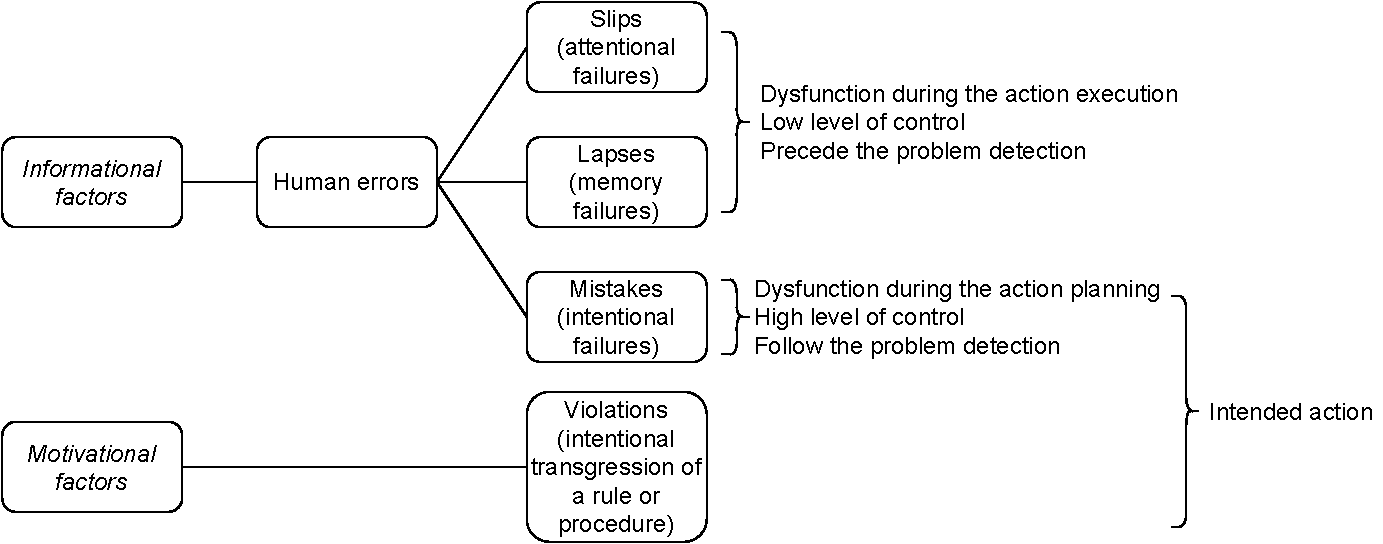
\includegraphics[width=\linewidth]{figures/chapter1/reason-errors.pdf}
 	\caption{Summary and simplification of the failure classification (Generic Error-Modelling System (GEMS) and violations) developed by Reason~\cite{reason_1990_human}. (Illustration by Kathleen Belhassein)}
 	\label{chap1:fig:err}
 \end{figure}


\subsection{Repair strategies}
In psychology or philosophy, there are not a lot of works on what happens once an error has been made during a joint action. Conversation Analysis investigated repair, which is a way to correct a misunderstanding or an error during an interaction or an action. The ability to engage in repair is essential in interactions. Indeed, errors and misunderstandings are likely to arise and people should find ways to correct them. Generally, they are classified in four categories in CA \cite{schegloff_1977_preference,wooffitt_2008_conversation}:
\begin{bulletList}
	\item Self-initiated self-repair: Repair is both initiated and carried out by the responsible of the trouble
	\item Other-initiated self-repair: The responsible of the trouble takes care of the repair himself but the trouble have been pointed out by the other
	\item Self-initiated other-repair: The responsible of the trouble signals that a repair is needed and get the other one to repair (\eg he forgot a name and asks for help to remember)
	\item Other-initiated other-repair: The one not responsible of the trouble initiates and carries out the repair. This is closest to what is conventionally understood as ``correction''.
\end{bulletList}

\ifdefined\included
\else
\bibliographystyle{acm}
\bibliography{These}
\end{document}
\fi

\ifdefined\included
\else
\documentclass[a4paper,11pt,twoside]{StyleThese}
\usepackage{amsmath,amssymb, amsthm}             % AMS Math
\usepackage[T1]{fontenc}
\usepackage[utf8x]{inputenc}
\usepackage{babel}
\usepackage{datetime}

\usepackage{silence}

\WarningFilter{minitoc(hints)}{W0023}
\WarningFilter{minitoc(hints)}{W0028}
\WarningFilter{minitoc(hints)}{W0030}

\usepackage{lmodern}
\usepackage{tabularx}
%\usepackage{tabular}
\usepackage{multirow}
\usepackage{xspace}

\usepackage{subfig}
\usepackage[inline]{enumitem}

\usepackage{hhline}
\usepackage[left=1.5in,right=1.3in,top=1.1in,bottom=1.1in,includefoot,includehead,headheight=13.6pt]{geometry}
\renewcommand{\baselinestretch}{1.05}

% Table of contents for each chapter

\usepackage[nottoc, notlof, notlot]{tocbibind}
\usepackage{minitoc}
\setcounter{minitocdepth}{2}
\mtcindent=15pt
% Use \minitoc where to put a table of contents

\usepackage{aecompl}

% Glossary / list of abbreviations

\usepackage[intoc]{nomencl}
\iftoggle{ThesisInEnglish}{%
\renewcommand{\nomname}{Glossary}
}{ %
\renewcommand{\nomname}{Liste des Abréviations}
}

\usepackage{etoolbox}
\renewcommand\nomgroup[1]{%
  \item[\bfseries
  \ifstrequal{#1}{A}{Number Sets}{%
  \ifstrequal{#1}{G}{Agents Beliefs and Action Models}{%
  \ifstrequal{#1}{N}{Navigation}{%
  \ifstrequal{#1}{O}{Ontology}{%
  \ifstrequal{#1}{R}{Referring Expression Generation}{%
  \ifstrequal{#1}{Z}{Controllable and Uncontrollable Agents Task Planning}{}}}}}}%
]}

\makenomenclature



% My pdf code

\usepackage{ifpdf}

\ifpdf
  \usepackage[pdftex]{graphicx}
  \DeclareGraphicsExtensions{.jpg}
  \usepackage[pagebackref,hyperindex=true]{hyperref}
  \usepackage{tikz}
  \usetikzlibrary{arrows,shapes,calc}
\else
  \usepackage{graphicx}
  \DeclareGraphicsExtensions{.ps,.eps}
  \usepackage[dvipdfm,pagebackref,hyperindex=true]{hyperref}
\fi

\graphicspath{{.}{images/}}

%% nicer backref links. NOTE: The flag ThesisInEnglish is used to define the
% language in the back references. Read more about it in These.tex

\iftoggle{ThesisInEnglish}{%
\renewcommand*{\backref}[1]{}
\renewcommand*{\backrefalt}[4]{%
\ifcase #1 %
(Not cited.)%
\or
(Cited in page~#2.)%
\else
(Cited in pages~#2.)%
\fi}
\renewcommand*{\backrefsep}{, }
\renewcommand*{\backreftwosep}{ and~}
\renewcommand*{\backreflastsep}{ and~}
}{%
\renewcommand*{\backref}[1]{}
\renewcommand*{\backrefalt}[4]{%
\ifcase #1 %
(Non cité.)%
\or
(Cité en page~#2.)%
\else
(Cité en pages~#2.)%
\fi}
\renewcommand*{\backrefsep}{, }
\renewcommand*{\backreftwosep}{ et~}
\renewcommand*{\backreflastsep}{ et~}
}

% Links in pdf
\usepackage{color}
\definecolor{linkcol}{rgb}{0,0,0.4} 
\definecolor{citecol}{rgb}{0.5,0,0} 
\definecolor{linkcol}{rgb}{0,0,0} 
\definecolor{citecol}{rgb}{0,0,0}
% Change this to change the informations included in the pdf file

\hypersetup
{
bookmarksopen=true,
pdftitle="Endowing the robot with the abilities to control and evaluate its contribution to a human-robot joint action",
pdfauthor="Amandine MAYIMA", %auteur du document
pdfsubject="Thèse", %sujet du document
%pdftoolbar=false, %barre d'outils non visible
pdfmenubar=true, %barre de menu visible
pdfhighlight=/O, %effet d'un clic sur un lien hypertexte
colorlinks=true, %couleurs sur les liens hypertextes
pdfpagemode=None, %aucun mode de page
pdfpagelayout=SinglePage, %ouverture en simple page
pdffitwindow=true, %pages ouvertes entierement dans toute la fenetre
linkcolor=linkcol, %couleur des liens hypertextes internes
citecolor=citecol, %couleur des liens pour les citations
urlcolor=linkcol %couleur des liens pour les url
}

% definitions.
% -------------------

\setcounter{secnumdepth}{3}
\setcounter{tocdepth}{2}

% Some useful commands and shortcut for maths:  partial derivative and stuff

\newcommand{\pd}[2]{\frac{\partial #1}{\partial #2}}
\def\abs{\operatorname{abs}}
\def\argmax{\operatornamewithlimits{arg\,max}}
\def\argmin{\operatornamewithlimits{arg\,min}}
\def\diag{\operatorname{Diag}}
\newcommand{\eqRef}[1]{(\ref{#1})}

\usepackage{rotating}                    % Sideways of figures & tables
%\usepackage{bibunits}
%\usepackage[sectionbib]{chapterbib}          % Cross-reference package (Natural BiB)
%\usepackage{natbib}                  % Put References at the end of each chapter
                                         % Do not put 'sectionbib' option here.
                                         % Sectionbib option in 'natbib' will do.
\usepackage{fancyhdr}                    % Fancy Header and Footer

% \usepackage{txfonts}                     % Public Times New Roman text & math font
  
%%% Fancy Header %%%%%%%%%%%%%%%%%%%%%%%%%%%%%%%%%%%%%%%%%%%%%%%%%%%%%%%%%%%%%%%%%%
% Fancy Header Style Options

\pagestyle{fancy}                       % Sets fancy header and footer
\fancyfoot{}                            % Delete current footer settings

%\renewcommand{\chaptermark}[1]{         % Lower Case Chapter marker style
%  \markboth{\chaptername\ \thechapter.\ #1}}{}} %

%\renewcommand{\sectionmark}[1]{         % Lower case Section marker style
%  \markright{\thesection.\ #1}}         %

\fancyhead[LE,RO]{\bfseries\thepage}    % Page number (boldface) in left on even
% pages and right on odd pages
\fancyhead[RE]{\bfseries\nouppercase{\leftmark}}      % Chapter in the right on even pages
\fancyhead[LO]{\bfseries\nouppercase{\rightmark}}     % Section in the left on odd pages

\let\headruleORIG\headrule
\renewcommand{\headrule}{\color{black} \headruleORIG}
\renewcommand{\headrulewidth}{1.0pt}
\usepackage{colortbl}
\arrayrulecolor{black}

\fancypagestyle{plain}{
  \fancyhead{}
  \fancyfoot{}
  \renewcommand{\headrulewidth}{0pt}
}

%\usepackage{MyAlgorithm}
%\usepackage[noend]{MyAlgorithmic}
\usepackage{algorithm}
\usepackage[noend]{algpseudocode}
\usepackage{comment}
\usepackage[ED=MITT-InfoTel, Ets=INSA]{tlsflyleaf}
%%% Clear Header %%%%%%%%%%%%%%%%%%%%%%%%%%%%%%%%%%%%%%%%%%%%%%%%%%%%%%%%%%%%%%%%%%
% Clear Header Style on the Last Empty Odd pages
\makeatletter

\def\cleardoublepage{\clearpage\if@twoside \ifodd\c@page\else%
  \hbox{}%
  \thispagestyle{empty}%              % Empty header styles
  \newpage%
  \if@twocolumn\hbox{}\newpage\fi\fi\fi}

\newcommand*{\algrule}[1][\algorithmicindent]{%
	\makebox[#1][l]{%
		\hspace*{.2em}% <------------- This is where the rule starts from
		\vrule height .75\baselineskip depth .25\baselineskip
	}
}

%%% to have lines in algorithm, from stackexchange
\newcount\ALG@printindent@tempcnta
\def\ALG@printindent{%
	\ifnum \theALG@nested>0% is there anything to print
	\ifx\ALG@text\ALG@x@notext% is this an end group without any text?
	% do nothing
	\else
	\unskip
	% draw a rule for each indent level
	\ALG@printindent@tempcnta=1
	\loop
	\algrule[\csname ALG@ind@\the\ALG@printindent@tempcnta\endcsname]%
	\advance \ALG@printindent@tempcnta 1
	\ifnum \ALG@printindent@tempcnta<\numexpr\theALG@nested+1\relax
	\repeat
	\fi
	\fi
}
% the following line injects our new indent handling code in place of the default spacing
\patchcmd{\ALG@doentity}{\noindent\hskip\ALG@tlm}{\ALG@printindent}{}{\errmessage{failed to patch}}
\patchcmd{\ALG@doentity}{\item[]\nointerlineskip}{}{}{} % no spurious vertical space
% end vertical rule patch for algorithmicx

\makeatother
 
%%%%%%%%%%%%%%%%%%%%%%%%%%%%%%%%%%%%%%%%%%%%%%%%%%%%%%%%%%%%%%%%%%%%%%%%%%%%%%% 
% Prints your review date and 'Draft Version' (From Josullvn, CS, CMU)
\newcommand{\reviewtimetoday}[2]{\special{!userdict begin
    /bop-hook{gsave 20 710 translate 45 rotate 0.8 setgray
      /Times-Roman findfont 12 scalefont setfont 0 0   moveto (#1) show
      0 -12 moveto (#2) show grestore}def end}}
% You can turn on or off this option.
% \reviewtimetoday{\today}{Draft Version}
%%%%%%%%%%%%%%%%%%%%%%%%%%%%%%%%%%%%%%%%%%%%%%%%%%%%%%%%%%%%%%%%%%%%%%%%%%%%%%% 

\newenvironment{maxime}[1]
{
\vspace*{0cm}
\hfill
\begin{minipage}{0.5\textwidth}%
%\rule[0.5ex]{\textwidth}{0.1mm}\\%
\hrulefill $\:$ {\bf #1}\\
%\vspace*{-0.25cm}
\it 
}%
{%

\hrulefill
\vspace*{0.5cm}%
\end{minipage}
}

\let\minitocORIG\minitoc
\renewcommand{\minitoc}{\minitocORIG \vspace{1.5em}}

\usepackage{multirow}
%\usepackage{slashbox}

\newenvironment{bulletList}%
{ \begin{list}%
	{\tiny$\bullet$}%
	{\setlength{\labelwidth}{25pt}%
	 \setlength{\leftmargin}{30pt}%
	 \setlength{\itemsep}{-0.5em}}}%
{ \end{list} }

\newenvironment{inlineEnumerate}
{\begin{enumerate*} [label={(\arabic*)}] }
{\end{enumerate*}}

\theoremstyle{definition}
\newtheorem{definition}{Definition}
\renewcommand{\epsilon}{\varepsilon}

% centered page environment

\newenvironment{vcenterpage}
{\newpage\vspace*{\fill}\thispagestyle{empty}\renewcommand{\headrulewidth}{0pt}}
{\vspace*{\fill}}

\newenvironment{asl}{\ttfamily\begin{tabbing}~~~\=$\leftarrow$ \= ~~~ \=
		\kill}{\end{tabbing}}

\usepackage{tablefootnote}

\theoremstyle{plain}
\newtheorem{constraint}{Constraint}[section]

\algnewcommand\algorithmicforeach{\textbf{for each}}
\algnewcommand\algorithmicin{\textbf{in}}
\algdef{S}[FOR]{ForEach}[2]{\algorithmicforeach\ #1\ \algorithmicin\ #2\ \algorithmicdo}

\algnewcommand\algorithmicforkxor{\textbf{do fork-join-xor}}
\algnewcommand\algorithmicendforkxor{\textbf{end fork-join-xor}}
\algdef{SE}{ForkXor}{EndForkXor}{\algorithmicforkxor}{\algorithmicendforkxor}


\usepackage{listings}
\lstset{
	frame=single,
	captionpos=b,
	breaklines=true,
	basicstyle=\ttfamily,
	numberstyle=\color{black},
	tabsize=2,
	mathescape=true,
	literate=%
		{â}{{\^a}}1
}

\lstdefinestyle{inline}{
	frame=none,
	aboveskip=\smallskipamount,
	belowskip=\smallskipamount,
}

\lstdefinestyle{OwlTurtle}{
	language=C,
	tabsize=4,
	basicstyle=\scriptsize\ttfamily,
	keywordstyle=\bfseries\color{darkgray},
	morekeywords={rdf:type, rdfs:domain, rdfs:subPropertyOf, rdfs:range, :hasSubtask, :DecompositionUsedBy, rdfs:subClassOf, :hasDecomposition, owl:inverseOf, htn_actions:hasEffect, rdfs:label},
	alsoletter=:
}

\lstdefinestyle{aslDef}{
	frame=none,
%	breaklines=false,
	%xleftmargin=.1\textwidth, xrightmargin=.1\textwidth
}

\fancypagestyle{example}{%
	\fancyhead[LE]{\bfseries\thepage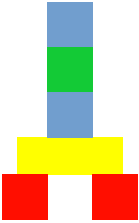
\includegraphics[scale=0.20]{figures/chapter2/task_goal.pdf}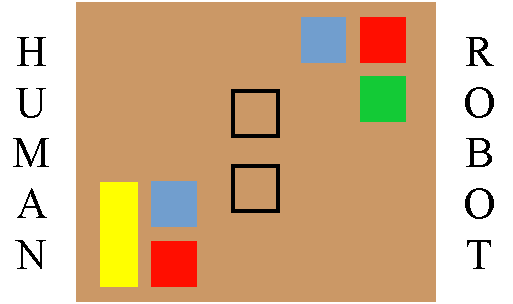
\includegraphics[scale=0.18]{figures/chapter2/task_setup_mini.pdf}}   
	\fancyhead[RO]{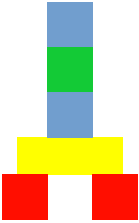
\includegraphics[scale=0.20]{figures/chapter2/task_goal.pdf}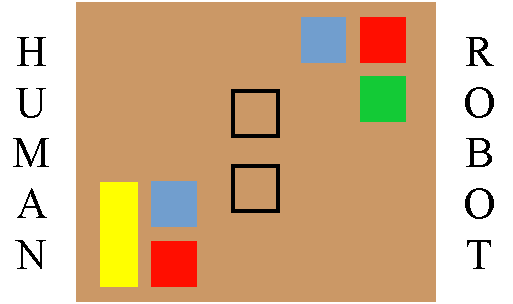
\includegraphics[scale=0.18]{figures/chapter2/task_setup_mini.pdf}\bfseries\thepage}  
	\fancyhead[RE]{\bfseries\nouppercase{\leftmark}}      % Chapter in the right on even pages
	\fancyhead[LO]{\bfseries\nouppercase{\rightmark}}     % Section in the left on odd pages
}%

\usepackage{pdfpages}
\usepackage{makecell}
\usepackage{pdflscape} 
\usepackage{mathtools}
\usepackage[section]{placeins}
\usepackage{afterpage}

%%%%%%%% my commands
\newcommand{\etal}{\textit{et al}.}
\newcommand{\ie}{\textit{i.e.}, }
\newcommand{\eg}{\textit{e.g.}, }
\newcommand{\fact}[3]{\mbox{\textit{#1}(#2, #3)}}
\newcommand{\circledtext}[1]{\raisebox{.5pt}{\textcircled{\raisebox{-.9pt} {#1}}}}
\newcommand{\sparql}{\textsc{SPARQL}}

\newcommand{\algConst}[1]{${\scriptscriptstyle #1}$}
\newcommand{\algNormTextSub}[2]{$\text{#1}_{#2}$}

\newcommand{\aslnumber}[1]{$#1$}
\newcommand{\aslstring}[1]{\textsf{#1}}
\newcommand{\aslvar}[1]{\textcolor{purple}{\textit{#1}}}
\newcommand{\asllabel}[1]{\textbf{#1}}
\newcommand{\annotation}[1]{{\footnotesize #1}}
\newcommand{\rulebody}[1]{\mbox{\hspace{.05\linewidth}}\begin{minipage}[t]{0.9\linewidth}#1.\end{minipage}}
\newcommand{\context}[1]{\begin{minipage}[t]{0.9\linewidth}#1\end{minipage}}
\newcommand{\planbody}[1]{\begin{minipage}[t]{0.9\linewidth}#1.\end{minipage}}
\newcommand{\Jason}[0]{\textbf{\textit{Jason}}}
\newcommand{\sn}{\mbox{\large\textbf{\texttt{\textasciitilde}}}}


\sloppy
\begin{document}
	\setcounter{chapter}{1} %% Numéro du chapitre précédent ;)
	\dominitoc
	\faketableofcontents
	\fi


\chapter{The ``special case'' of Human-Robot Interaction}\label{chapter:chap2}
\minitoc

In the previous chapter, we took an interest in the human-human interactions and collaboration in order to be aware of the elements to consider when devising a collaborative robot. 

In this chapter, first in Section~\ref{chap2:sec:soc_inter}, we will analyze how the \acrshort{hri} field defines and frames human-robot social interaction. Then, in Section~\ref{chap2:sec:hri_ja}, in the context of a collaborative work with philosophers and psychologists, we reviewed some elements of joint action and collaboration which have already been implemented in robotics.

\section{Human-Robot Social Interactions}\label{chap2:sec:soc_inter}

Now that we have seen how social interactions look like when happening between humans, we are going to see the different ways the human-robot interaction field divided and categorized interactions. It is possible to define an interaction according to its duration as we will show in Section~\ref{chap2:subsec:inter_lengths}. Then, inside the interaction, what are the different temporal phases? We will see it in Section~\ref{chap2:subsec:inter_div}. Finally, in Section~\ref{chap2:subsec:inter_hier}, we will take an interest in a different way to segment interactions: with hierarchical levels.

\subsection{Interaction durations}\label{chap2:subsec:inter_lengths}
\paragraph{Human-Robot Short-term Interactions}
\cite{zheng_2013_designing} defined a human-robot \emph{short-term interaction}~ based on the Unified Theories of Cognition of Newell~\citep{newell_1994_unified}. A short-term interaction corresponds to the ``cognitive band'' of cognition, during which they focus on individual utterances and speech acts for interactions that last for tens of seconds. They left aside longer-term interactions that can be in the ``rational band'' (minutes to hours) or the ``social band'' (days to months).

\cite{gaschler_2012_modelling} deployed a bartender robot and defined a short-term interaction as being a customer ordering a drink – from the attention request towards the bartender to the closing of interaction by payment and exchange of polite phrases.

\cite{iocchi_2015_personalized} used the \emph{short-term} to refer to short interactions and that are focused on only one particular communicative objective, avoiding long and complex interactions.

\cite{sanelli_2017_short} gave three characteristics to a short-term human-robot interaction: 
\begin{inlineEnumerate}
	\item users are not familiar with the robot,
	\item each interaction happens with a different user, and
	\item interaction is short in time.
\end{inlineEnumerate} Then, the robot has not memory of past interactions.

\paragraph{Human-Robot Long-term Interactions}
A survey has been provided by \cite{leite_2013_social} about long-term human-robot interactions, where long-term means, most of the time, several interactions between the same human and robot. They defined four contexts for which social robots\footnote{actually, some of the robots featured in the survey are not social robots such as a Roomba or the Personal Exploration Rover (PER)} for long-term interaction have been designed: health care and therapy, education, work environment and public spaces, and people's homes. 

For example, \cite{kanda_2007_two} performed a field trial at an elementary school in Japan for two months. The children were able to interact with the robot for 32 days in total, during 30 minutes after lunch. The robot could switch between one hundred pre-defined behaviors (\eg hugging, shaking hand or singing) but not all of them were available during the first interactions with a human. Indeed, they had integrated a pseudo-development mechanism, \ie the more a child interacts with the robot, the more different behaviours the robot displays to that child. Also, the robot confided personal-themed matters to children who have often interacted with it (\eg ``I don't like the cold''). These abilities allowed the robot to maintain the children's interest even after the first week whereas in a first experiment where the robot's behavior was the same all along the two months, most children stopped to interact with the robot from the second week. 

In their discussion, Kanda \etal{} raised an interesting question: ``How Long Should \textquoteleft Long-Term\textquoteright{} Be?'' They found out that some authors considered that two months is a long-term interaction. They also pointed that some Human-Computer Interaction studies on long-term interaction last five weeks. In their survey, Leite \etal{} gave their point of view, which seems well thought. Indeed, argued that it is more important to look at the number of interaction sessions and the duration of these sessions (a five minutes-interaction is different from a one hour-interaction). For them, an interaction can be considered as long-term when the user becomes familiarized with the robot to a point that their perception of such robot is not biased by the novelty effect anymore. This definition raises another question: when does user’s familiarization with the robot become stable? But we will not discuss it here.

\subsection{Interactions organized in phases}\label{chap2:subsec:inter_div}
Among work on short-term or long-term interactions, some authors organized interactions in phases which have sometimes similarities with the phases of social interactions described in Section~\ref{chap1:sec:soc_int}.

\cite{gockley_2005_designing} organized an interaction in three phases: greeting, core of the interaction and departure. In the greeting phase, Valerie, the robot receptionist, greets people who might be interested in engaging in conversation. Thus, people are classified into ``attentional'' states:
\begin{bulletList}
	\item present (people a bit far and moving): Valerie does not pay attention to them
	\item attending (people closer): Valerie greets them
	\item engages (people next to the desk but on the side): Valerie acknowledges their presence but does not expect input from them
	\item interacting (people in front of the keyboard): Valerie prompts them for input if they are not typing.
\end{bulletList}
In the core of interaction, either Valerie can tell her (fictive) story or chat. Her story is subjective and evolve over time. It is about her social life, her lounge singing career, her therapy business, and her job as a receptionist. Furthermore, Valerie has a chatbot system which is very simple. Inputs from visitors are from a keyboard, for easier control and reliability. Finally, at departure, when a person leaves the ``interacting'' region, Valerie signals the end of the interaction by saying ``goodbye''. 

\cite{kidd_2008_robots} presented robot which is a weigh loss coach. They introduced here the notion of states of relationship. They are three: initial (for the first few days of interaction), normal, repair. According to the state of relationship, the robot answers/questions/speech will not be the same. \cite{kasap_2012_building} designed their system so, to each user, corresponds an interaction session. Each session is composed of four dialogue phases: welcome, warm up, teach and farewell. The system has a memory of users and past interactions. In the memory, is recorded the context (initial state and goal), contents (events) and the outcome (goal succeeded or not). A bit similar to the relationship state defined by \cite{kidd_2008_robots}, they defined a notion that they call relationship level. It is computed based of the emotional interactions from the episodic memory associated to a user. It influences the mood level of the robot and then the facial expression and the speech.

In the work around a bartender robot, JAMES~\citep{gaschler_2012_modelling}, they organized the interaction in three phases (or states) but from two different viewpoints, the of the customer and the one of the bartender. From the customer viewpoints, the phases are: 
\begin{inlineEnumerate}
	\item attention request towards bartender,
	\item ordering of one or more beverages, and
	\item closing of interaction by payment and exchange of polite phrases.
\end{inlineEnumerate} Then, in reaction of each phases, there are the ones from the bartender viewpoint:
\begin{inlineEnumerate}
	\item acknowledging the attention request,
	\item serving the ordered drink, and
	\item asking for payment.
\end{inlineEnumerate}
They left open the possibility to have sub-phases inside phases.

We can also find, in Lee \etal{}' work~\citep{lee_2012_personalization}, the notion of structure of interaction: interactions start with the vendor identifying the customer, greeting and engaging in small talk with the customer, engaging in the snack transaction, and then enacting social leave-taking.

\subsection{Hierarchical structures of interactions}\label{chap2:subsec:inter_hier}
Not only, interactions can be organized in phases but also in levels. For example, \cite{dautenhahn_2002_embodied, ogden_2001_interactional} defined two levels of approach for human-robot interactions, a global one and a local one. The \emph{global level approach} defines a unit of interaction as being relatively large (long sequences of interaction or large units of interaction), such as the script for a greeting as described by \cite{kendon_1990_conducting}. At this level, an interaction may be seen as a unit similar to a schema or script, in the computer/cognitive science senses of these terms. They named this level of interaction a ``Global Interactional Unit (GIU)''. 

Furthermore, a GIU can be divided in phases, each of which has associated behaviors. Behaviors have meaning and their meaning depends on the phase in which they occur, the context (\eg a ‘wave hello’ vs. a ‘wave goodbye’). Their \emph{local level approach} is a much smaller unit, often as simple as an action and a response to that action. They claimed that this view of interaction has the advantage of greater flexibility and robustness compared to the globally structured view. Flexibility is a result of the possibility of specifying acts that may occur in many global interactional structures. But, they are aware that, as contextual details are ignored, the ability to assign a specific meaning to an action is lost.

In his thesis, \cite{kuo_2012_designing} insists about this flexibility and the re-usability. A lower level of design is more appropriate for reuse. For him, a unit of interaction corresponds to an ``interaction cue'' (or social cue) that a robot can perceive and act upon or express in an interaction. These cues can be verbal, non-verbal, or a combination of both (multi-modal interaction). A complete episode of interaction should be constructed through composition of interaction cues with some common patterns repeated over the course of the interaction (\eg awareness of human presence).

\begin{comment}
	
\subsection{Patterns of Interaction}\label{chap2:subsec:inter_patt}
Before talking about design patterns or interaction patterns, Goffman argued that human interactions follow a specific ``order'' and characterized a number of patterns in which people interact, such as how greetings unfold and how people leave an interaction~\cite{goffman_1983_interaction}.

Kahn \etal{} introduced design patterns~\cite{kahn_2008_design}, that they will later called interaction patterns in~\cite{kahn_2010_validating}, inspired from computer science. They proposed rules to follow using them and eight patterns. The most important ideas are that a sequence of patterns has to be well ordered and that patterns can be hierarchical. 
The 8 patterns: 
\begin{bulletList}
	\item The initial introduction: largely scripted, conventionally-established verbal and behavioral repertoire to recognize the other, inquire politely about the other, engage in some physical acknowledgment (\eg handshake)
	\item Didactic communication: one-way communication of information 
	\item In motion together: walk together
	\item Personal interests and history: sharing of personal interests and history with others
	\item Recovering from mistakes: creates the potential for both parties to maintain a social affiliation following the mistake
	\item Reciprocal turn-taking in game contextual: taking turns with one another when playing games
	\item Physical intimacy: to engage in holding or touching or embracing
	\item Claiming unfair treatment or wrongful harms: allows to make claim to its moral standing
\end{bulletList}


Following the same idea and going further, Sauppé and Mutlu introduced the interaction blocks~\cite{sauppe_2014_design}. Compared to Kahn’s work, they created a pattern language and a tool/environment to design human-robot interaction. To conceive their patterns, they collected and analyzed data from 5 kinds of interaction scenarios: Conversation, Collaboration, Instruction, Interview and Storytelling.
Then, they identified common interaction structures, which served as ``design interaction patterns'':
\begin{bulletList}
	\item Introductory monologue: A short introduction can be used to introduce other participants to a scenario by giving an overview of the remainder of the interaction or it can be a greeting for example.
	\item Question and Answer: A question is a sentence meant to elicit information from other participants. An answer is the response to a question that aims to satisfy the questioning participant’s curiosity.
	\item Generic Comment and Personal Comment: A comment is a short statement offering the speaker’s opinion. Comments are either generic (\eg, ``Wow'') or personal (\eg, ``I tried that and didn’t like it'').
	\item Monologue and Generic Comment: A monologue is a longer form of speech during which no response is expected.(\eg telling of a story). Although monologues expect no response, listeners may occasionally offer unsolicited commentary.
	\item Instruction and Action: An instruction is a command offered by one participant to direct the actions of another participant. The proper response to this instruction is often an action, although the action might follow the instruction with a delay depending on whether it is an appropriate time to perform that action
	\item Finished Comment: Upon the completion of the goals of the scenario, one or more of the participants will note that the scenario is completed by offering a finished comment.
	\item Wait: One pattern implicit in all scenarios involving two or more participants is the wait pattern.
\end{bulletList}
Finally, they designed a software to easily implement those patterns in a robot.

In his thesis, Kuo criticizes Kahn’s work~\cite{kuo_2012_designing}. He says that these patterns involve sequences of interaction cues and should be decomposed to a lower level for detailed design and reuse. He proposed his own patterns:
\begin{bulletList}
	\item Human presence detection: detect when there is a person who might be interested in
	\item Showing interest for interaction: express the robot’s awareness of a user’s presence around it and its interest and willingness to interact
	\item User’s attention on the robot: Know when a user is paying attention to the robot in an interaction and its information on its screen
	\item User identification by face: Provides the fundamental block for personal service and social interaction by recognizing the human counterpart in an interaction
\end{bulletList}
He checked the validity of his patterns with the analysis of Problem statement, Context of Use, Interaction Modality, Combination with Other Patterns, Technical Performance and Limitations, User Feedback and User’s Perception, Resulting Interactive Behavior.

Finally, Peltason and Wrede also based their work on design patterns from computer science, specifically applied to dialogue here~\cite{peltason_2010_pamini}. To name a few of them: Simple action request, Interaction opening, Interaction closing, Clarification. During interaction, the registered patterns are employed in a flexible way by admitting that patterns can be interrupted by other patterns and possibly resumed later which leads to interleaving patterns. By default, simpler patterns are permitted to be nested within temporally extended patterns.

\end{comment}


\bigskip

The work presented here in Section~\ref{chap2:sec:soc_inter}, dealt with human-robot social interactions. They considered the interactions from different points of view. Thus, several dimensions should be taken into account when designing, structuring a human-robot social interaction: how long, how often do we expect the robot to interact with a particular person? what is the context, what are the interaction phases the robot is expected to meet? are there multiple levels in the interaction?

Now, we will reduce our scope, going from social interactions to joint action in \acrshort{hri}. 

\section{Human-Robot Interaction and Joint Action}\label{chap2:sec:hri_ja}
The study of human-human joint action is important to understand how to make robots better companions and partners for humans. However, it does not mean that they should imitate humans, as they are machines, they have their own abilities and have to develop their own strategies~\citep{bradshaw_2017_human} (\eg displaying an arrow on the floor while navigating~\citep{chadalavada_2015_mind, coovert_2014_spatial}).

In the context of the JointAction4HRI project\footnote{\url{https://jointaction4hri.laas.fr/}}, a non-exhaustive review of existing robotic systems integrating but also recognizing in humans joint action mechanisms has been done, focusing on joint attention, communication to facilitate coordination, and \acrlong{tom}.

\subsection{Joint Attention in HRI}
Joint attention is essential to joint action (see Section~\ref{chap1:subsubsec:joint_att}). Some authors showed that a robot initiating (\ie triggering the attention focus of the partner on the object of interest)~\citep{imai_2003_physical}, responding to (\ie gaze following of the partner's gaze or gesture)~\citep{yu_2010_investigating}, and ensuring joint attention (\ie monitoring of the other's attention)~\citep{huang_2010_joint} improves the task performance and is perceived as more natural. Moreover, some studies have shown the benefit of eye-gaze management, and by this way, joint attention management, whether to help coordination during shared plan execution \citep{lallee_2013_cooperative} or to help the human with decision-making \citep{boucher_2010_facilitation, boucher_2012_reach}. Thus, human pointing gesture recognition as been investigated such as in~\citep{nickel_2007_visual} or eye-gaze signaling(\eg \citep{staudte_2009_visual} or see review~\citep{admoni_2017_social}).

\subsection{Communication to Facilitate Coordination in HRI}

As seen in Section~\ref{chap1:sec:comm}, communication is important for joint action. It is useful to negotiate, guide, question or realign the beliefs between agents as divergences might occur~\citep{cohen_1991_teamwork}. In this section, we will see how robots can do to communicate and understand communications about: 
\begin{inlineEnumerate}
	\item their internal state or the human partner's one, and
	\item intentions.
\end{inlineEnumerate}

\paragraph{Internal state communication -- Expressions}
It is not always obvious for the human to know what the robot is ``thinking'', \ie to know in what internal state is the robot (\eg everything is ok, a failure occurred, etc). The robot also needs to be able to estimate human mental states. Roboticists developed different ways to do so. 

We found that robot communicating their internal state using lights, dialogue, gestures/moves or facial expressions has been developed. Some of them are also able to analyze human face or voice to detect their emotion or expression. \cite{kim_2010_computational} designed a robot using all these features to generate expressions according to its knowledge about the task execution state, in a task where the robot has to guess the object the person has in mind among pre-defined several objects through questions and answers. Expressions are generated based on as set of criteria. For example, when the robot computes that it is in an unexpected state, it generates surprise. Moreover, they endowed the robot the ability to discriminate between the human partner's happiness, sadness and anger. 

In the same spirit, we can find a robot recognizing and generating expressions through voice, in relation to the task state and goal~\citep{scheutz_2006_utility}. 

Finally, we have to mention the work of Breazeal which investigated a lot display of emotions/expressions in human-robot interaction. We can distinguish two types of communication:
\begin{inlineEnumerate}
	\item a robot, which has a caregiver, has a motivation system in order to regulate the interaction intensity of its caregiver by expressing eight emotions with facial expressions~\citep{breazeal_1998_motivational, breazeal_2004_function}, and
	\item a robot has the ability to recognize four communication intents (approval, attentional bid, prohibition, soothing) and to react to them through speech~\citep{breazeal_2002_regulation, breazeal_2003_emotion}
\end{inlineEnumerate}

\paragraph{Communication of intentions} As explained in Section~\ref{chap1:subsubsec:coord_smooth}, coordination smoothers facilitate the prediction and legibility of a partner's action. For example, investigations about how the robot could communicate its intention during navigation have been carried out. 

Some authors chose to have the robot communicating its intention using lights~\citep{szafir_2015_communicating}, comparing this method with a communication using the head orientation and finding it better~\citep{may_2015_show}. 

Others worked on making the robot navigation legible, improving its predictability by the human~\citep{dragan_2013_legibility, alami_2006_toward,khambhaita_2016_head}. A last method to communication navigation intention is by projecting arrows on the floor as well as a map~\citep{chadalavada_2015_mind, coovert_2014_spatial}.  Not only robot navigation should be legible but also its gestures, when handing over an object to the human~\citep{sisbot_2012_human}, or opening a door~\citep{takayama_2011_expressing} for example. Finally, a lot of work can be found on human gestures recognition so the robot could prediction human's action intentions (\eg\citep{barros_2017_dynamic, chang_2018_effects}).

\subsection{Theory of Mind in HRI}\label{chap2:subsec:tom_hri}
\acrfull{tom} is related to joint action as shown in Section~\ref{chap1:sec:tom}. One of the first work to bind robotics and \acrshort{tom} is \cite{scassellati_2002_theory}. He proposed a model of a \acrshort{tom} implementation for a robot, inspired by two models from psychology: Leslie’s Model of Theory of Mind~\citep{leslie_1984_spatiotemporal} and Baron-Cohen’s Model of Theory of Mind~\citep{baron-cohen_1995_mindblindness}. Scassellati's model focused on two abilities: to make the distinction between animate and inanimate visual stimuli (following Leslie's perceptual world division into animate and inanimate spheres), and to identify gaze direction (enabling the shared attention mechanism as emphasized by Baron-Cohen). 

Over the years, others tried to tackle this issue, especially focusing on perspective-taking abilities. For example, \cite{hiatt_2010_cognitive} designed and implemented a model simulating a human with the ability to deal with false beliefs. They demonstrated it with the Sally--Anne test presented in Section~\ref{chap1:sec:tom}. \cite{milliez_2014_framework} endowed a robot with the ability to pass the Sally--Anne test, constructing a semantic representation of the world based on its estimation of the human's point of view.

Perspective-taking abilities have been used in robotics for several purposes. \cite{berlin_2006_perspective} presented a simulated robot able to take the visual perspective of a human teacher (the virtual camera) and showed how this ability could be used for learning in human-robot interaction. \cite{hiatt_2011_accommodating} presented a humanoid robot reasoning on possible beliefs the human partner could have endowing the robot with the ability to deal with uncertainty about the estimation of the human's beliefs. In another work, perspective-taking allows the robot to solve ambiguous references to an object~\citep{ros_2010_solving}. Others make use of perspective-taking to improve human action recognition~\citep{johnson_2005_perceptual}. Endowing a robot with a perspective-taking ability can also serve to support the implementation of an autobiographical memory (a meaningful stored knowledge acquired during interactions)~\citep{pointeau_2017_role}. Finally, it can also be a way to help the robot to elaborate plans, adding communication actions to solve divergent beliefs~\citep{warnier_2012_robot}, to explain plans to the human with a level of details depending on their knowledge~\citep{milliez_2016_using} or to manage shared plans execution~\citep{devin_2016_implemented}.

\section{Conclusion}

The presented work are very interested and important for the \acrshort{hri} community. We focused on joint attention and communication because of the project context then we explored \acrshort{tom} as it is an important aspect for the supervision. What is brought out when exploring the joint action aspects in \acrshort{hri} is that the models and implementations proposed often lack a more general vision of joint action, focusing on a particular aspect~\citep{belhassein_2020_horizontal}. We tried to take this into account and to tackle this issue when devising \acrshort{jahrvis}.
 


%\subsection{Failures in HRI}
%Honig and Oron-Gilad studied the different types of failures that could happen during a human-robot interaction and proposed a classification of these~\cite{honig_2018_understanding} based on a meticulous review, illustrated with Figure~\ref{chap2:fig:err_hri}.
%
%\begin{figure}[!ht]
%	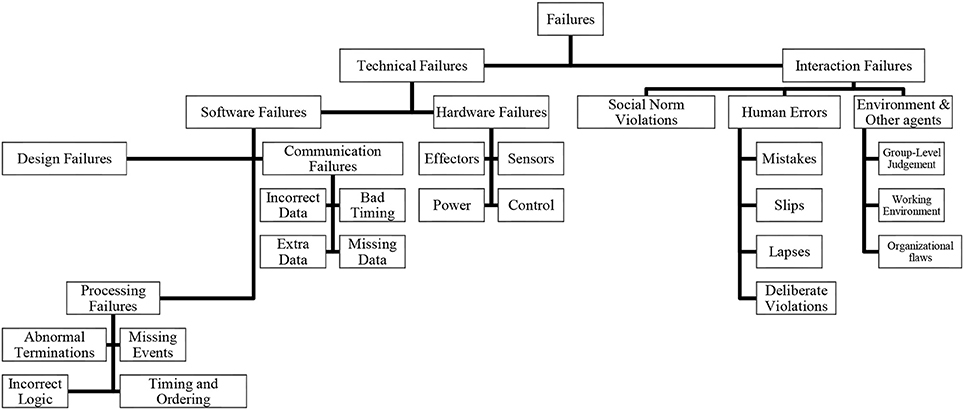
\includegraphics[width=\linewidth]{figures/chapter1/failures_hri.jpg}
%	\caption{Classification of failures in HRI, realized by Honig and Oron-Gilad~\cite{honig_2018_understanding}.}
%	\label{chap2:fig:err_hri}
%\end{figure}
%
%\subsubsection{Communicating about Failures}
%When something unexpected happens during the interaction, either because of a human failure, a robot failure or an external event, robots might need to communicate about it. We identified two common ways to communicate about a failure: facial expressions and speech. We can notice a less common way proposed by Kwon \etal{} which developed a robot communicating about its incapability to execute a manipulation tasks thanks to the execution of an ``attempt motion'', expressing what it cannot do and why to its human partner (\eg lifting its elbow to communicate that it is trying to lift the cup, but the cup is too heavy for it)~\cite{kwon_2018_expressing}. 
%
%\paragraph{Facial expressions} Breazeal and colleagues investigated the expression of the robot's confusion through facial expressions. For example, in~\cite{breazeal_2002_regulation, breazeal_2003_emotion} humans take into account the robot expressive feedback to assess when the robot ``understand'' them. If the wrong expression appeared, they often speak in an exaggerated way to correct the ``misunderstanding''. Hamacher \etal{} developed a robot  displaying a facial expression after having dropped an egg when preparing an omelet with a human~\cite {hamacher_2016_believing}. Reyes \etal{} proposed a robot displaying a negative facial expression when an error occurs~\cite{reyes_2015_positive}. In a work by Silva \etal, the robot decision-making and error detection/handling processes are influenced by the perceived human emotions and the robot can display facial expressions when the human persists in a error~\cite{silva_2016_combining}.
%
%\paragraph{Speech} Most of the time, when speech is involved, it is not only to communicate about the failure but also to initiate a repair strategy. 
%
%\subsubsection{Robot Repair Strategies}
%To communicate about a failure is not enough to be able to continue the task or the interaction. A collaborative robot needs repair strategies. Some authors proposed simple strategies while some others developed more complex ones. In~\cite{li_2006_computational}, when the robot detects a failure in its understanding of the human utterance and gesture, it triggers its repair mechanism that leads the robot to ask questions to the human in order to help it disambiguate the utterance/gesture. In~\cite{morales_2019_interaction}, there were two possibilities when a failure happened: the human had an ``assistance opportunity'' (\ie failure case that caused no risk to person or property) before the failure occurrence or not. People were more willing to help the robot in case of failure with an assistance opportunity. Knepper \etal{} proposed a robot, when encountering a failure, able to request help from a human -- which might not be aware of the context. After receiving help, it resumes its autonomous task execution~\cite{knepper_2015_recovering}. Lee \etal{} compared three recovering strategies after a robot failure (but based on videos and not a real robot) to see which one was preferred by the humans: (1) apology (\ie robot apologies for service failure), (2) compensation (\ie robot provides compensation, such as an exchange, a refund, or a discount coupon), (3) option (\ie robot provides human with alternative actions to achieve their goals)~\cite{lee_2010_gracefully}. All strategies had a positive effect (even if not the same). Spexard \etal{} developed three repair strategies according to the type of failure for their robot: (1) when the robot encounters an internal issue, it informs the human about the break-down and asking them a reboot or to contact a technician, (2) it can generate appropriate speech related to error messages from its sensor, \eg the robot informs the human of the reason why it can not move and asks them for help, and (3) the robot asks for a reset if it thinks that the information it has about a human does not seem to be right~\cite{spexard_2008_oops}. Mutlu \etal{} performed a user study to compare three repair strategies in a task where the robot gives instructions to the human in an assembly task~\cite{mutlu_2013_coordination}. The strategies are: (1) ``no repair'' (\ie the robot detects an error but waits without answering to the human's questions), (2) ``simple repair'' (\ie the robot answers by yes or no to the human yes/no questions, for other questions it repeats the instruction), and (3) ``humanlike-repair'' (\ie the robot gives the appropriate information to human, triggered either by a human request, or failure or hesitancy detection). The last strategy was the preferred one by the participants.

\ifdefined\included
\else
\bibliographystyle{acm}
\bibliography{These}
\end{document}
\fi

\part{The Challenge of Social Interaction Management}\label{part:part2}
\begin{partintro}
	We explore robotic architectures and \acrfull{bdi} which have inspired us to implement the architecture in which \acrshort{jahrvis} in the puppeteer.
	
	Then, we present \acrfull{dacobot}, our architecture dedicated to human-robot collaboration and the components composing it. Each component has been thought to be used in a \acrshort{hri} context.
\end{partintro}	
\ifdefined\included
\else
\documentclass[a4paper,11pt,twoside]{StyleThese}
\usepackage{amsmath,amssymb, amsthm}             % AMS Math
\usepackage[T1]{fontenc}
\usepackage[utf8x]{inputenc}
\usepackage{babel}
\usepackage{datetime}

\usepackage{silence}

\WarningFilter{minitoc(hints)}{W0023}
\WarningFilter{minitoc(hints)}{W0028}
\WarningFilter{minitoc(hints)}{W0030}

\usepackage{lmodern}
\usepackage{tabularx}
%\usepackage{tabular}
\usepackage{multirow}
\usepackage{xspace}

\usepackage{subfig}
\usepackage[inline]{enumitem}

\usepackage{hhline}
\usepackage[left=1.5in,right=1.3in,top=1.1in,bottom=1.1in,includefoot,includehead,headheight=13.6pt]{geometry}
\renewcommand{\baselinestretch}{1.05}

% Table of contents for each chapter

\usepackage[nottoc, notlof, notlot]{tocbibind}
\usepackage{minitoc}
\setcounter{minitocdepth}{2}
\mtcindent=15pt
% Use \minitoc where to put a table of contents

\usepackage{aecompl}

% Glossary / list of abbreviations

\usepackage[intoc]{nomencl}
\iftoggle{ThesisInEnglish}{%
\renewcommand{\nomname}{Glossary}
}{ %
\renewcommand{\nomname}{Liste des Abréviations}
}

\usepackage{etoolbox}
\renewcommand\nomgroup[1]{%
  \item[\bfseries
  \ifstrequal{#1}{A}{Number Sets}{%
  \ifstrequal{#1}{G}{Agents Beliefs and Action Models}{%
  \ifstrequal{#1}{N}{Navigation}{%
  \ifstrequal{#1}{O}{Ontology}{%
  \ifstrequal{#1}{R}{Referring Expression Generation}{%
  \ifstrequal{#1}{Z}{Controllable and Uncontrollable Agents Task Planning}{}}}}}}%
]}

\makenomenclature



% My pdf code

\usepackage{ifpdf}

\ifpdf
  \usepackage[pdftex]{graphicx}
  \DeclareGraphicsExtensions{.jpg}
  \usepackage[pagebackref,hyperindex=true]{hyperref}
  \usepackage{tikz}
  \usetikzlibrary{arrows,shapes,calc}
\else
  \usepackage{graphicx}
  \DeclareGraphicsExtensions{.ps,.eps}
  \usepackage[dvipdfm,pagebackref,hyperindex=true]{hyperref}
\fi

\graphicspath{{.}{images/}}

%% nicer backref links. NOTE: The flag ThesisInEnglish is used to define the
% language in the back references. Read more about it in These.tex

\iftoggle{ThesisInEnglish}{%
\renewcommand*{\backref}[1]{}
\renewcommand*{\backrefalt}[4]{%
\ifcase #1 %
(Not cited.)%
\or
(Cited in page~#2.)%
\else
(Cited in pages~#2.)%
\fi}
\renewcommand*{\backrefsep}{, }
\renewcommand*{\backreftwosep}{ and~}
\renewcommand*{\backreflastsep}{ and~}
}{%
\renewcommand*{\backref}[1]{}
\renewcommand*{\backrefalt}[4]{%
\ifcase #1 %
(Non cité.)%
\or
(Cité en page~#2.)%
\else
(Cité en pages~#2.)%
\fi}
\renewcommand*{\backrefsep}{, }
\renewcommand*{\backreftwosep}{ et~}
\renewcommand*{\backreflastsep}{ et~}
}

% Links in pdf
\usepackage{color}
\definecolor{linkcol}{rgb}{0,0,0.4} 
\definecolor{citecol}{rgb}{0.5,0,0} 
\definecolor{linkcol}{rgb}{0,0,0} 
\definecolor{citecol}{rgb}{0,0,0}
% Change this to change the informations included in the pdf file

\hypersetup
{
bookmarksopen=true,
pdftitle="Endowing the robot with the abilities to control and evaluate its contribution to a human-robot joint action",
pdfauthor="Amandine MAYIMA", %auteur du document
pdfsubject="Thèse", %sujet du document
%pdftoolbar=false, %barre d'outils non visible
pdfmenubar=true, %barre de menu visible
pdfhighlight=/O, %effet d'un clic sur un lien hypertexte
colorlinks=true, %couleurs sur les liens hypertextes
pdfpagemode=None, %aucun mode de page
pdfpagelayout=SinglePage, %ouverture en simple page
pdffitwindow=true, %pages ouvertes entierement dans toute la fenetre
linkcolor=linkcol, %couleur des liens hypertextes internes
citecolor=citecol, %couleur des liens pour les citations
urlcolor=linkcol %couleur des liens pour les url
}

% definitions.
% -------------------

\setcounter{secnumdepth}{3}
\setcounter{tocdepth}{2}

% Some useful commands and shortcut for maths:  partial derivative and stuff

\newcommand{\pd}[2]{\frac{\partial #1}{\partial #2}}
\def\abs{\operatorname{abs}}
\def\argmax{\operatornamewithlimits{arg\,max}}
\def\argmin{\operatornamewithlimits{arg\,min}}
\def\diag{\operatorname{Diag}}
\newcommand{\eqRef}[1]{(\ref{#1})}

\usepackage{rotating}                    % Sideways of figures & tables
%\usepackage{bibunits}
%\usepackage[sectionbib]{chapterbib}          % Cross-reference package (Natural BiB)
%\usepackage{natbib}                  % Put References at the end of each chapter
                                         % Do not put 'sectionbib' option here.
                                         % Sectionbib option in 'natbib' will do.
\usepackage{fancyhdr}                    % Fancy Header and Footer

% \usepackage{txfonts}                     % Public Times New Roman text & math font
  
%%% Fancy Header %%%%%%%%%%%%%%%%%%%%%%%%%%%%%%%%%%%%%%%%%%%%%%%%%%%%%%%%%%%%%%%%%%
% Fancy Header Style Options

\pagestyle{fancy}                       % Sets fancy header and footer
\fancyfoot{}                            % Delete current footer settings

%\renewcommand{\chaptermark}[1]{         % Lower Case Chapter marker style
%  \markboth{\chaptername\ \thechapter.\ #1}}{}} %

%\renewcommand{\sectionmark}[1]{         % Lower case Section marker style
%  \markright{\thesection.\ #1}}         %

\fancyhead[LE,RO]{\bfseries\thepage}    % Page number (boldface) in left on even
% pages and right on odd pages
\fancyhead[RE]{\bfseries\nouppercase{\leftmark}}      % Chapter in the right on even pages
\fancyhead[LO]{\bfseries\nouppercase{\rightmark}}     % Section in the left on odd pages

\let\headruleORIG\headrule
\renewcommand{\headrule}{\color{black} \headruleORIG}
\renewcommand{\headrulewidth}{1.0pt}
\usepackage{colortbl}
\arrayrulecolor{black}

\fancypagestyle{plain}{
  \fancyhead{}
  \fancyfoot{}
  \renewcommand{\headrulewidth}{0pt}
}

%\usepackage{MyAlgorithm}
%\usepackage[noend]{MyAlgorithmic}
\usepackage{algorithm}
\usepackage[noend]{algpseudocode}
\usepackage{comment}
\usepackage[ED=MITT-InfoTel, Ets=INSA]{tlsflyleaf}
%%% Clear Header %%%%%%%%%%%%%%%%%%%%%%%%%%%%%%%%%%%%%%%%%%%%%%%%%%%%%%%%%%%%%%%%%%
% Clear Header Style on the Last Empty Odd pages
\makeatletter

\def\cleardoublepage{\clearpage\if@twoside \ifodd\c@page\else%
  \hbox{}%
  \thispagestyle{empty}%              % Empty header styles
  \newpage%
  \if@twocolumn\hbox{}\newpage\fi\fi\fi}

\newcommand*{\algrule}[1][\algorithmicindent]{%
	\makebox[#1][l]{%
		\hspace*{.2em}% <------------- This is where the rule starts from
		\vrule height .75\baselineskip depth .25\baselineskip
	}
}

%%% to have lines in algorithm, from stackexchange
\newcount\ALG@printindent@tempcnta
\def\ALG@printindent{%
	\ifnum \theALG@nested>0% is there anything to print
	\ifx\ALG@text\ALG@x@notext% is this an end group without any text?
	% do nothing
	\else
	\unskip
	% draw a rule for each indent level
	\ALG@printindent@tempcnta=1
	\loop
	\algrule[\csname ALG@ind@\the\ALG@printindent@tempcnta\endcsname]%
	\advance \ALG@printindent@tempcnta 1
	\ifnum \ALG@printindent@tempcnta<\numexpr\theALG@nested+1\relax
	\repeat
	\fi
	\fi
}
% the following line injects our new indent handling code in place of the default spacing
\patchcmd{\ALG@doentity}{\noindent\hskip\ALG@tlm}{\ALG@printindent}{}{\errmessage{failed to patch}}
\patchcmd{\ALG@doentity}{\item[]\nointerlineskip}{}{}{} % no spurious vertical space
% end vertical rule patch for algorithmicx

\makeatother
 
%%%%%%%%%%%%%%%%%%%%%%%%%%%%%%%%%%%%%%%%%%%%%%%%%%%%%%%%%%%%%%%%%%%%%%%%%%%%%%% 
% Prints your review date and 'Draft Version' (From Josullvn, CS, CMU)
\newcommand{\reviewtimetoday}[2]{\special{!userdict begin
    /bop-hook{gsave 20 710 translate 45 rotate 0.8 setgray
      /Times-Roman findfont 12 scalefont setfont 0 0   moveto (#1) show
      0 -12 moveto (#2) show grestore}def end}}
% You can turn on or off this option.
% \reviewtimetoday{\today}{Draft Version}
%%%%%%%%%%%%%%%%%%%%%%%%%%%%%%%%%%%%%%%%%%%%%%%%%%%%%%%%%%%%%%%%%%%%%%%%%%%%%%% 

\newenvironment{maxime}[1]
{
\vspace*{0cm}
\hfill
\begin{minipage}{0.5\textwidth}%
%\rule[0.5ex]{\textwidth}{0.1mm}\\%
\hrulefill $\:$ {\bf #1}\\
%\vspace*{-0.25cm}
\it 
}%
{%

\hrulefill
\vspace*{0.5cm}%
\end{minipage}
}

\let\minitocORIG\minitoc
\renewcommand{\minitoc}{\minitocORIG \vspace{1.5em}}

\usepackage{multirow}
%\usepackage{slashbox}

\newenvironment{bulletList}%
{ \begin{list}%
	{\tiny$\bullet$}%
	{\setlength{\labelwidth}{25pt}%
	 \setlength{\leftmargin}{30pt}%
	 \setlength{\itemsep}{-0.5em}}}%
{ \end{list} }

\newenvironment{inlineEnumerate}
{\begin{enumerate*} [label={(\arabic*)}] }
{\end{enumerate*}}

\theoremstyle{definition}
\newtheorem{definition}{Definition}
\renewcommand{\epsilon}{\varepsilon}

% centered page environment

\newenvironment{vcenterpage}
{\newpage\vspace*{\fill}\thispagestyle{empty}\renewcommand{\headrulewidth}{0pt}}
{\vspace*{\fill}}

\newenvironment{asl}{\ttfamily\begin{tabbing}~~~\=$\leftarrow$ \= ~~~ \=
		\kill}{\end{tabbing}}

\usepackage{tablefootnote}

\theoremstyle{plain}
\newtheorem{constraint}{Constraint}[section]

\algnewcommand\algorithmicforeach{\textbf{for each}}
\algnewcommand\algorithmicin{\textbf{in}}
\algdef{S}[FOR]{ForEach}[2]{\algorithmicforeach\ #1\ \algorithmicin\ #2\ \algorithmicdo}

\algnewcommand\algorithmicforkxor{\textbf{do fork-join-xor}}
\algnewcommand\algorithmicendforkxor{\textbf{end fork-join-xor}}
\algdef{SE}{ForkXor}{EndForkXor}{\algorithmicforkxor}{\algorithmicendforkxor}


\usepackage{listings}
\lstset{
	frame=single,
	captionpos=b,
	breaklines=true,
	basicstyle=\ttfamily,
	numberstyle=\color{black},
	tabsize=2,
	mathescape=true,
	literate=%
		{â}{{\^a}}1
}

\lstdefinestyle{inline}{
	frame=none,
	aboveskip=\smallskipamount,
	belowskip=\smallskipamount,
}

\lstdefinestyle{OwlTurtle}{
	language=C,
	tabsize=4,
	basicstyle=\scriptsize\ttfamily,
	keywordstyle=\bfseries\color{darkgray},
	morekeywords={rdf:type, rdfs:domain, rdfs:subPropertyOf, rdfs:range, :hasSubtask, :DecompositionUsedBy, rdfs:subClassOf, :hasDecomposition, owl:inverseOf, htn_actions:hasEffect, rdfs:label},
	alsoletter=:
}

\lstdefinestyle{aslDef}{
	frame=none,
%	breaklines=false,
	%xleftmargin=.1\textwidth, xrightmargin=.1\textwidth
}

\fancypagestyle{example}{%
	\fancyhead[LE]{\bfseries\thepage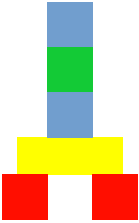
\includegraphics[scale=0.20]{figures/chapter2/task_goal.pdf}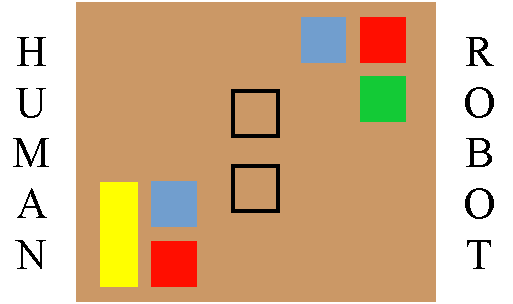
\includegraphics[scale=0.18]{figures/chapter2/task_setup_mini.pdf}}   
	\fancyhead[RO]{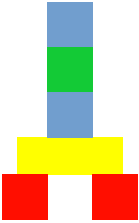
\includegraphics[scale=0.20]{figures/chapter2/task_goal.pdf}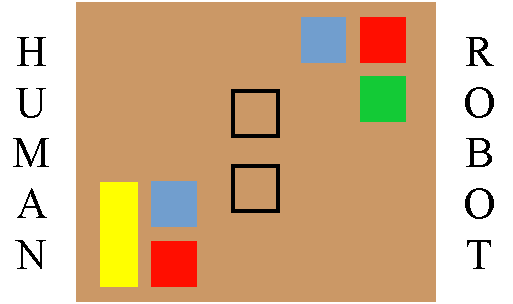
\includegraphics[scale=0.18]{figures/chapter2/task_setup_mini.pdf}\bfseries\thepage}  
	\fancyhead[RE]{\bfseries\nouppercase{\leftmark}}      % Chapter in the right on even pages
	\fancyhead[LO]{\bfseries\nouppercase{\rightmark}}     % Section in the left on odd pages
}%

\usepackage{pdfpages}
\usepackage{makecell}
\usepackage{pdflscape} 
\usepackage{mathtools}
\usepackage[section]{placeins}
\usepackage{afterpage}

%%%%%%%% my commands
\newcommand{\etal}{\textit{et al}.}
\newcommand{\ie}{\textit{i.e.}, }
\newcommand{\eg}{\textit{e.g.}, }
\newcommand{\fact}[3]{\mbox{\textit{#1}(#2, #3)}}
\newcommand{\circledtext}[1]{\raisebox{.5pt}{\textcircled{\raisebox{-.9pt} {#1}}}}
\newcommand{\sparql}{\textsc{SPARQL}}

\newcommand{\algConst}[1]{${\scriptscriptstyle #1}$}
\newcommand{\algNormTextSub}[2]{$\text{#1}_{#2}$}

\newcommand{\aslnumber}[1]{$#1$}
\newcommand{\aslstring}[1]{\textsf{#1}}
\newcommand{\aslvar}[1]{\textcolor{purple}{\textit{#1}}}
\newcommand{\asllabel}[1]{\textbf{#1}}
\newcommand{\annotation}[1]{{\footnotesize #1}}
\newcommand{\rulebody}[1]{\mbox{\hspace{.05\linewidth}}\begin{minipage}[t]{0.9\linewidth}#1.\end{minipage}}
\newcommand{\context}[1]{\begin{minipage}[t]{0.9\linewidth}#1\end{minipage}}
\newcommand{\planbody}[1]{\begin{minipage}[t]{0.9\linewidth}#1.\end{minipage}}
\newcommand{\Jason}[0]{\textbf{\textit{Jason}}}
\newcommand{\sn}{\mbox{\large\textbf{\texttt{\textasciitilde}}}}


\sloppy
\begin{document}
	\setcounter{chapter}{2} %% Numéro du chapitre précédent ;)
	\dominitoc
	\faketableofcontents
	\fi

\chapter{Architectures for Collaborative Robots, Decision and Execution}\label{chapter:chap3}
\chaptermark{Architectures for Decision and Execution}
\minitoc
Robots are machine which need to perceive, decide and act. There are multiple ways to endow a robot with such abilities, with different levels of complexity. When a robot has a complex and generic software architecture, based on models which might be inspired from other fields like psychology, philosophy, neurology, it is referred to as cognitive robot or autonomous robots or intelligent robot...We are interested in such architectures but designed to be implemented in collaborative robots. And, we take an interest in a particular function of these architecture: the decision-making, the supervision of the task, of the interaction.

\section{Existing Architectures for Collaborative Robots}\label{chap3:sec:archi}
``An integrated cognitive architecture can be defined as a single system that is capable of producing all aspects of behaviour, while remaining constant across various domains and knowledge bases''~\cite[p.~104]{chong_2007_integrated}. Kotseruba and Tsotsos reviewed cognitive architectures starting 40 years ago until nowadays. They accounted around three hundred of them and chose to focus their review on 84~\cite{kotseruba_2020_40}. However, the term \emph{cognitive architecture} often refers to an architecture modeling human cognition~\cite{howes_1997_role} and what interest us is to endow robots with cognitive and interactive abilities, not always basing ourselves on human cognition.  

Some cognitive architectures such as ACT-R has been adapted for human-robot interaction (ACT-R/E)~\cite{trafton_2013_act}. The architecture aims at simulating how humans think, perceive and act in the world, strongly based on theory of mind. It is interesting but to understand humans is not enough to make the robot a good collaborators for them, as it lacks abilities concerning the human-aware task and action execution. 

A very complete architecture, CRAM, dealing with problems such as manipulation, perception, plans or beliefs management has been developed by Beetz \etal~\cite{beetz_2010_cram}. However, this architecture is more designed for a robot acting alone than a robot acting in collaboration with a human.

The work of Scheutz and colleagues is compelling, as they proposed a generic architecture, DIARC, for cognitive robots collaborating with humans~\cite{scheutz_2006_utility,scheutz_2019_overview}. In this context, it handles perception, dialogue and different kind of actions. But, the architecture lacks real modeling and awareness of the human at each level.

Rossi \etal{} presented in \cite{rossi_2013_extensible} an architecture to handle multi-modal interaction. In their system, users are able to express their instructions as combinations of different modalities considering that redundancy can be useful. The system is build upon a multi-layered late fusion approach, based on classification. In addition, the system is designed in a way to be easily extensible and easy to modify (\eg possibility to add or remove a modality, possibility to change the classification strategies). The system has been used for example to handle pick-place-carry tasks interacting with a robot through gestures and speech. However, this is for robots following human orders only, and not handling planning and plan execution.

Another architecture worth to be mentioned is the DAC-h3 architecture by Moulin-Frier, Fischer \etal, inspired from biology~\cite{moulin_2017_dac}. It is designed for a robot maintaining social interactions with humans, able to tell narratives and to acquire knowledge thanks to its interactions with humans. As it is mainly dedicated to knowledge acquisition and expression, it lacks planning and execution abilities.

As part of the Platform-Independent Cooperative Human Robot Interaction System, Lallee \etal{} proposed an original architecture for learning and executing shared plans~\cite{lallee_2012_towards}. They developed a way to encode actions in terms of perceptual changes based on motor primitives descriptions. That way, the robot is able to learn new actions as perceptions. Their actions can take several arguments (\eg AGENT put the OBJECT on the RECIPIENT) which enables the system to react and generalize when faced to a new context. The system takes as inputs spoken language interaction and visual perception. It is very interesting but focuses on robots learning objects, actions and plans and not really on collaborative tasks handling. 

Finally, there is the architecture developed and implemented by Lemaignan and colleagues for collaborative robots. All deliberative components of the architecture are human-aware~\cite{lemaignan_2017_artificial}, \ie all of components except the sensorimotor layer. This architecture is based on the philosophical BDI model developed by Bratman~\cite{bratman_1987_intention,bratman_1988_plans}. It has 3 main concepts defined as the following in computer science:
\begin{bulletList}
	\item \emph{Beliefs}: They are a representation of the agent’s knowledge about the world. ``[They] can be viewed as the informative component of system state''~\cite[p.~313]{rao_1995_bdi}. It is not the word ``knowledge'' that has been chosen to define this concept because what the agent perceives of the environment is in fact the likely state of the environment. There is no certainty, its sensors are not accurate or could malfunction. This way of distinguish knowledge and beliefs is one that can be found in the literature of distributed computing~\cite{lamarre_1994_knowledge}.
	\item \emph{Desires}\footnote{In one of the first implementation, PRS, ``Goals'' notion was used instead of ``Desires''~\cite{georgeff_1989_decision}, then they use it in a interchangeable way in~\cite{georgeff_1991_modeling} and finally choose ``Desires''~\cite{rao_1995_bdi} with the definition given in the AI literature, \eg desires can be many at any instant and may be mutually incompatible. Therefore, a goal will be a chosen desire~\cite{cohen_1990_intention} and concurrent goals are consistent.}: They are a representation of the motivational state of the system. They provide ``information about the objectives to be accomplished or, more generally, what priorities or payoffs are associated with the various current objectives''~\cite{rao_1995_bdi}. 
	\item \emph{Intentions}: They are a representation of the currently chosen course of action (plan). It is the deliberative component of the system. The selected course(s) of action are determined with a deliberative function, according to the beliefs and desires~\cite{rao_1995_bdi}.
\end{bulletList}



\section{The new LAAS Architecture -- DACOBOT}\label{chap3:sec:rob_archi}

In this section, we present an overview of the robotic architecture, \acrfull{dacobot}, that we collaboratively developed with Guillaume Sarthou and Guilhem Buisan. This architecture model, shown in Figure~\ref{chap3:fig:archi}, has been inspired by the architecture developed by Lemaignan and colleagues~\cite{lemaignan_2017_artificial}, mentioned in the previous section. These architectures are descendant of one of the first architectures for autonomous robots, developed by Alami \etal{}~\cite{alami_1998_architecture}. They have a common characteristic: they are divided into three levels, the decisional level, the execution level and the functional level. Well, these three levels can be compared to the levels presented in the theoretical framework developed by Pacherie and presented in Section~\ref{chap1:subsubsec:neuro_seg}, which is a strong advantage for a robotic architecture dedicated to \acrshort{hri}.

\subsection{Specificities}

All the architectures presented in Section~\ref{chap3:sec:archi} are very interesting but we decided to focus on the last one presented, developed by Lemaignan \etal{}. It seemed relevant to us to pursue this work started in our lab by expanding the components features and refining, consolidating the interactions between these components. The component names and functions of both architectures are the same but most of the implementations are all new and the way they rely on, interact with each other, is as well. All the components of the \acrshort{dacobot} are designed to be human-aware, making the global system human-aware, which is quite rare.

With this architecture, we focus on a given type of \acrlong{hri}: collaborative tasks, joint actions. In this context, the human and the robot share a common space and exchange information through multiple modalities (speech, gesture, gaze). The robot should be able to act on its environment, by manipulating objects and navigate among humans. This function is assured by the Motion Planners and Excutors presented in Section~\ref{chap3:subsubsec:motion}. In order to be aware of its environment, the robot needs perception modalities which are handled by the sensorimotor layer, it can be cameras, lasers, motion capture, force sensors, etc. To avoid each component having to process the data itself in order to be able to use them, the Situation Assessment, presented in Section~\ref{chap3:subsubsec:sa} converts them from geometric data to symbolic data. Moreover, it endows the robot's visual perspective-taking (see Section~\ref{chap1:subsec:tom}). Then, these data are stored in \acrlong{kb}s which are introduced in Section~\ref{chap3:subsubsec:kb}, one for the robot and another for the human. Finally, the heart of the architecture, the decision-making process is located in the Supervisor which is the focus of Chapters~\ref{chapter:chap5} and~\ref{chapter:chap6}. In order to make its decisions, the Supervisor relies on the \acrshort{kb}s, the communication through the \acrfull{nlp} and especially the Task Planners presented in Section~\ref{chap3:subsubsec:task_planner}. Once the decision made, it controls the robot through the Motion Planners and Executors and the \acrshort{nlp}. All communication between the components goes through ROS~\cite{quigley_2009_ros}.

\begin{figure}[!ht]
	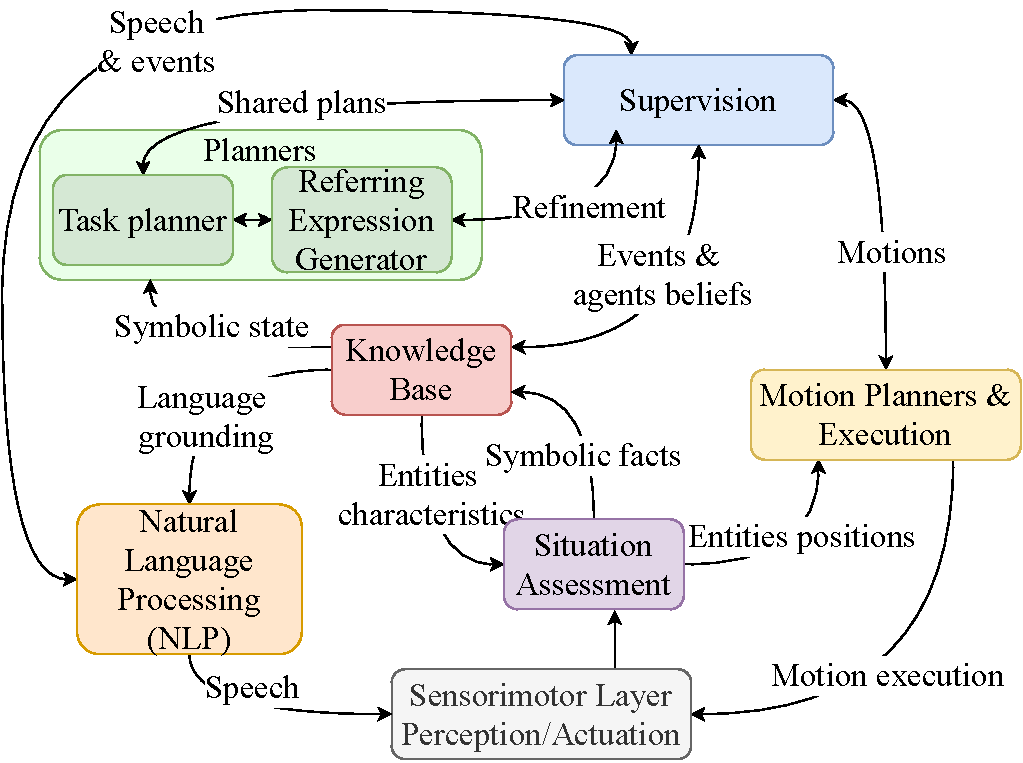
\includegraphics[width=\linewidth]{figures/chapter2/archi_overview.pdf}
	\caption{Overview of the \acrfull{dacobot}.}
	\label{chap3:fig:archi}
\end{figure}

\subsection{Architecture components}

\subsubsection{Situation Assessment}\label{chap3:subsubsec:sa}
The Situation Assessment has two roles:
\begin{enumerate}
	\item  to gather different perceptual information and build a geometric representation of the world (\ie elements have associated 3D coordinates), composed of objects and agents; from this world representation, the module runs reasoning processes to interpret it in terms of symbolic statements between the objects themselves and between the involved agents and the objects. Such component can be implemented with frameworks like Toaster~\cite{milliez_2014_framework} or Underworld~\cite{lemaignan_2018_underworlds}.
	\item estimate the human's perspective and build an estimation of their world representation; it is the first step allowing to implement the theory of mind principles (see Section~\ref{chap1:subsec:tom}).
\end{enumerate}

Thus, the Situation Assessment outputs data, which we call \textit{symbolic facts}, such as \fact{isOnTopOf}{cube\_1}{cube\_3} or \fact{isReachableBy}{cube\_2}{human\_0}. The first element of this triplet is called the property, the second one is the subject and the last one is the object.

\subsubsection{Knowledge Bases}\label{chap3:subsubsec:kb}

Knowledge management is central in a robotic architecture. As this architecture is specific to \acrshort{hri}, the knowledge handling should be as well. Indeed, during an interaction, belief divergences may arise between agents and thus how this should be represented? Each agent, human and robot, should have their own knowledge base. Software developed by Guillaume Sarthou with whom we collaborated closely allow this. They are two of them: Ontologenius\footnote{\url{https://github.com/sarthou/ontologenius}}~\cite{sarthou_2019_ontologenius} for the semantic knowledge and Mementar\footnote{\url{https://github.com/sarthou/mementar}} for the episodic one. They are fully adapted to \acrshort{hri} applications by representing the robot's knowledge and the estimation of the partners' knowledge separately, which refers to the psychological concept of the ``self-other distinction'' as coined in joint action studies~\cite{pacherie_2012_agency}.  

\paragraph{Semantic knowledge base} stores common-sense knowledge based on three concepts, in the form of an ontology\footnote{An ontology is a way to represent knowledge}: (1) classes representing the possible types of entities known by the agent (\eg Cube is a class inheriting from the class Pickable), (2) properties which can denote both the attributes of objects (\eg the color) and the relations between the objects (\eg which object is on which other one), and (3) object instantiations also called individuals (\eg cube\_3 is an object present in the environment, of the class Cube).

It is in charge of representing the environment elements meaning, the objects' and agents' types (\eg a cube is an object), their applicable properties (\eg cube\_1 has color blue), the descriptions and parameters of the actions, a part of the language model with verbs or pronouns, and their names in natural language.
	
Besides, it is also in charge of representing the current symbolic world-state (the computed facts, \eg \fact{isOnTof}{cube\_2}{table\_1}) and thus the instantiation of the concepts in terms of physical (\eg this particular block) or abstract (\eg this particular action instance) entities. Moreover, it reasons on it, making deductions and links between facts, creating new ones (\eg after receiving \fact{isOnTof}{cube\_2}{table\_1} and it computes \fact{isUnder}{table\_1}{cube\_2}). Finally, it stores knowledge about activities grounded in space and time (\eg object\_1245 has been put on the table\_2 by robot (action ID 475)).

To access to the knowledge stored in Ontologenius, the Supervisor can make a request to know if a given fact exists or ask an information about a class, a property or an object instantiation (\eg the Supervisor can ask the human understandable name of pick\_action which is ``pick''). Another way is to subscribe to updates (addition or deletion) for given facts (\ie facts necessary to the task or the Supervisor functioning). It is useful for keeping updates about the environment and avoid to be snowed under too much data. For example, the Supervisor can ask to receive every update (addition or deletion) of any fact belonging to the type \fact{isOnTopOf}{Cube}{Table}. In this case, it will receive the addition of \fact{isOnTopOf}{cube\_2}{table\_1} but not of \fact{isOnTopOf}{spoon}{table\_1}. It is possible to either specify the class or individual of the subjects/objects that should be concerned by the subscription, or to receive every facts (\eg it can subscribe to receive additions of the human looking at the robot |[add]human_0$\lvert$isLookingAt$\lvert$robot| or to receive all updates about every objects that the human looks at |[?]human_0$\lvert$isLookingAt$\lvert$?|). The way the Supervisor chooses which fact it should receive is described in Chapter~\ref{chapter:chap6}.

\paragraph{Episodic knowledge base} is represented as a timeline, keeping track of the symbolic facts computed over time (\eg action ID 475 started at 3286 seconds and was over at 3290 seconds), either by the Situation Assessment, the Semantic Knowledge Base or the Supervisor. 


\subsubsection{Human-Aware Motion Planners and Execution}\label{chap3:subsubsec:motion}
The motion planners allow the robot to execute human-aware motion actions. According to the task needs, several planners might be involved for a same task. Indeed, in a task requiring object manipulation, the robot will need a motion planner able to plan for pick, place and drop actions, such as MoveIt\footnote{\url{https://moveit.ros.org/}} or GTP which is human-aware~\cite{waldhart_2016_novel}, and a home-made software handling the execution these trajectories\footnote{\url{https://github.com/YannickRiou/pr2_mtc}}. Moreover, in collaborative tasks, an agent might be led to hand over an object to their partner, in this case could be used a dedicated planner~\cite{mainprice_2012_sharing}. Finally, the robot might need to move in the environment, but when moving in a environment with humans, it should navigate being aware of them for safety and legibility. Thus, the robotic architecture should integrate co-navigation planner and executor such as HATEB-2~\cite{singamaneni_2020_hateb}. 

These planners produce trajectories and moves on request of the Supervisor. During execution, they sends feedbacks about the state execution, in this way the Supervisor can receive data about something going wrong or the estimated remaining time of execution. 

\subsubsection{Human-Aware Task Planner}\label{chap3:subsubsec:task_planner}
We can distinguish two situations in which a collaborative robot needs a human-aware task planner: 
\begin{inlineEnumerate}
	\item when it performs a task on its own but a human is nearby and so it should consider potential conflicting actions with them, and
	\item when it performs a task with a human.
\end{inlineEnumerate} 
In the first situation, it might consider asking the human's help whereas in the second one it needs to plan for both agents' actions. 

The human-aware task planners generate symbolic shared plans in which each agent, human and robot, has actions of the task assigned to them, depending on criteria such as programmer-defined costs, minimization of the human's effort, and their preferences and comfort. Such plans are constructed to be as respectful as possible of social constraints which benefits to the also human-aware Supervisor. However, the human is neither an agent that the planner can directly control or an agent that will know the complete plan. Thus, it allows the robot to plan by emulating the human decision, action, and reaction processes. 

We worked with two human-aware task planners: \acrfull{hatp}~\cite{lallement_2014_hatp} and \acrfull{hatpehda}~\cite{buisan_2021_human}.

The \acrfull{hatp} proposes a hierarchical approach to multi agents task planning. This \acrfull{htn}-based planner is able to elaborate a multi agents plan based on a single \acrshort{htn} tree. \acrshort{htn} planning aims at decomposing abstract tasks into primitive tasks by choosing from a list of available context-dependent refinements for each abstract task, ensuring that preconditions and effects of refined primitives tasks are satisfied throughout the created plan. This formalism is suitable for human-robot interactions as it allows the robot to communicate about the plan more easily. \acrshort{hatp} has been specially designed to integrate a number of features that are meant to promote the synthesis of plans that are acceptable by humans and easily if not trivially understandable by them. It allows to specify the humans and robot capabilities in terms of actions they can execute. Several aspects such as human preferences and comfort, estimation of human effort to achieve a task in a given context and ``social rules'' are used in a cost-based approach to build ``sufficiently good'' human-robot shared plans.

The \acrfull{hatpehda} also proposes a hierarchical approach to multi agents task planning. This approach relies on a representation of each agent considered by the planner, with their own beliefs, agenda, stream of execution and action model. The action models are represented as \acrshort{htn}s which are explored consecutively yet differently if the agent is controllable (robots) or uncontrollable but rational (humans). We highlight two main advantages over \acrshort{hatp}. The first one is the computation of conditional plans, allowing to anticipate situations where the human may perform multiple different actions equally making the plan progressing, or may decide to act or wait for the robot to act. Then, the decision of which branch of the plan to follow is postponed at execution time and handled by the Supervisor. Another advantage is to explicitly represent robot to human communication needs for beliefs alignment, goal sharing or action requests. Indeed, \acrshort{hatp} generates plans in which it is unknown what needs to be communicated to the human or what can be easily guessed (\ie which is predictable) by the human. Finally, like in \acrshort{hatp}, it is possible to define ``social costs functions''. By doing so, the planner can penalize non-acceptable sequence of robot actions (\eg serving a meal just after taking out the trash) or non-satisfactory human required contribution (\eg or requesting the human to perform small tasks multiple times instead of giving the big picture of the real task to perform).


\subsubsection{Supervision}
The Supervision is the puppet master of the system, embedding the robot high-level decisions, controlling its behavior and trying to react to contingencies, always considering the human it is interacting with. It is not standalone, relying on the components described above to be able to take decisions, be aware of the environment and make the robot moves.
\newline

After giving an overview of the components on which the supervision relies, we present the context in which we place ourselves for human-robot collaboration.



\ifdefined\included
\else
\bibliographystyle{acm}
\bibliography{These}
\end{document}
\fi
\ifdefined\included
\else
\documentclass[a4paper,11pt,twoside]{StyleThese}
\usepackage{amsmath,amssymb, amsthm}             % AMS Math
\usepackage[T1]{fontenc}
\usepackage[utf8x]{inputenc}
\usepackage{babel}
\usepackage{datetime}

\usepackage{silence}

\WarningFilter{minitoc(hints)}{W0023}
\WarningFilter{minitoc(hints)}{W0028}
\WarningFilter{minitoc(hints)}{W0030}

\usepackage{lmodern}
\usepackage{tabularx}
%\usepackage{tabular}
\usepackage{multirow}
\usepackage{xspace}

\usepackage{subfig}
\usepackage[inline]{enumitem}

\usepackage{hhline}
\usepackage[left=1.5in,right=1.3in,top=1.1in,bottom=1.1in,includefoot,includehead,headheight=13.6pt]{geometry}
\renewcommand{\baselinestretch}{1.05}

% Table of contents for each chapter

\usepackage[nottoc, notlof, notlot]{tocbibind}
\usepackage{minitoc}
\setcounter{minitocdepth}{2}
\mtcindent=15pt
% Use \minitoc where to put a table of contents

\usepackage{aecompl}

% Glossary / list of abbreviations

\usepackage[intoc]{nomencl}
\iftoggle{ThesisInEnglish}{%
\renewcommand{\nomname}{Glossary}
}{ %
\renewcommand{\nomname}{Liste des Abréviations}
}

\usepackage{etoolbox}
\renewcommand\nomgroup[1]{%
  \item[\bfseries
  \ifstrequal{#1}{A}{Number Sets}{%
  \ifstrequal{#1}{G}{Agents Beliefs and Action Models}{%
  \ifstrequal{#1}{N}{Navigation}{%
  \ifstrequal{#1}{O}{Ontology}{%
  \ifstrequal{#1}{R}{Referring Expression Generation}{%
  \ifstrequal{#1}{Z}{Controllable and Uncontrollable Agents Task Planning}{}}}}}}%
]}

\makenomenclature



% My pdf code

\usepackage{ifpdf}

\ifpdf
  \usepackage[pdftex]{graphicx}
  \DeclareGraphicsExtensions{.jpg}
  \usepackage[pagebackref,hyperindex=true]{hyperref}
  \usepackage{tikz}
  \usetikzlibrary{arrows,shapes,calc}
\else
  \usepackage{graphicx}
  \DeclareGraphicsExtensions{.ps,.eps}
  \usepackage[dvipdfm,pagebackref,hyperindex=true]{hyperref}
\fi

\graphicspath{{.}{images/}}

%% nicer backref links. NOTE: The flag ThesisInEnglish is used to define the
% language in the back references. Read more about it in These.tex

\iftoggle{ThesisInEnglish}{%
\renewcommand*{\backref}[1]{}
\renewcommand*{\backrefalt}[4]{%
\ifcase #1 %
(Not cited.)%
\or
(Cited in page~#2.)%
\else
(Cited in pages~#2.)%
\fi}
\renewcommand*{\backrefsep}{, }
\renewcommand*{\backreftwosep}{ and~}
\renewcommand*{\backreflastsep}{ and~}
}{%
\renewcommand*{\backref}[1]{}
\renewcommand*{\backrefalt}[4]{%
\ifcase #1 %
(Non cité.)%
\or
(Cité en page~#2.)%
\else
(Cité en pages~#2.)%
\fi}
\renewcommand*{\backrefsep}{, }
\renewcommand*{\backreftwosep}{ et~}
\renewcommand*{\backreflastsep}{ et~}
}

% Links in pdf
\usepackage{color}
\definecolor{linkcol}{rgb}{0,0,0.4} 
\definecolor{citecol}{rgb}{0.5,0,0} 
\definecolor{linkcol}{rgb}{0,0,0} 
\definecolor{citecol}{rgb}{0,0,0}
% Change this to change the informations included in the pdf file

\hypersetup
{
bookmarksopen=true,
pdftitle="Endowing the robot with the abilities to control and evaluate its contribution to a human-robot joint action",
pdfauthor="Amandine MAYIMA", %auteur du document
pdfsubject="Thèse", %sujet du document
%pdftoolbar=false, %barre d'outils non visible
pdfmenubar=true, %barre de menu visible
pdfhighlight=/O, %effet d'un clic sur un lien hypertexte
colorlinks=true, %couleurs sur les liens hypertextes
pdfpagemode=None, %aucun mode de page
pdfpagelayout=SinglePage, %ouverture en simple page
pdffitwindow=true, %pages ouvertes entierement dans toute la fenetre
linkcolor=linkcol, %couleur des liens hypertextes internes
citecolor=citecol, %couleur des liens pour les citations
urlcolor=linkcol %couleur des liens pour les url
}

% definitions.
% -------------------

\setcounter{secnumdepth}{3}
\setcounter{tocdepth}{2}

% Some useful commands and shortcut for maths:  partial derivative and stuff

\newcommand{\pd}[2]{\frac{\partial #1}{\partial #2}}
\def\abs{\operatorname{abs}}
\def\argmax{\operatornamewithlimits{arg\,max}}
\def\argmin{\operatornamewithlimits{arg\,min}}
\def\diag{\operatorname{Diag}}
\newcommand{\eqRef}[1]{(\ref{#1})}

\usepackage{rotating}                    % Sideways of figures & tables
%\usepackage{bibunits}
%\usepackage[sectionbib]{chapterbib}          % Cross-reference package (Natural BiB)
%\usepackage{natbib}                  % Put References at the end of each chapter
                                         % Do not put 'sectionbib' option here.
                                         % Sectionbib option in 'natbib' will do.
\usepackage{fancyhdr}                    % Fancy Header and Footer

% \usepackage{txfonts}                     % Public Times New Roman text & math font
  
%%% Fancy Header %%%%%%%%%%%%%%%%%%%%%%%%%%%%%%%%%%%%%%%%%%%%%%%%%%%%%%%%%%%%%%%%%%
% Fancy Header Style Options

\pagestyle{fancy}                       % Sets fancy header and footer
\fancyfoot{}                            % Delete current footer settings

%\renewcommand{\chaptermark}[1]{         % Lower Case Chapter marker style
%  \markboth{\chaptername\ \thechapter.\ #1}}{}} %

%\renewcommand{\sectionmark}[1]{         % Lower case Section marker style
%  \markright{\thesection.\ #1}}         %

\fancyhead[LE,RO]{\bfseries\thepage}    % Page number (boldface) in left on even
% pages and right on odd pages
\fancyhead[RE]{\bfseries\nouppercase{\leftmark}}      % Chapter in the right on even pages
\fancyhead[LO]{\bfseries\nouppercase{\rightmark}}     % Section in the left on odd pages

\let\headruleORIG\headrule
\renewcommand{\headrule}{\color{black} \headruleORIG}
\renewcommand{\headrulewidth}{1.0pt}
\usepackage{colortbl}
\arrayrulecolor{black}

\fancypagestyle{plain}{
  \fancyhead{}
  \fancyfoot{}
  \renewcommand{\headrulewidth}{0pt}
}

%\usepackage{MyAlgorithm}
%\usepackage[noend]{MyAlgorithmic}
\usepackage{algorithm}
\usepackage[noend]{algpseudocode}
\usepackage{comment}
\usepackage[ED=MITT-InfoTel, Ets=INSA]{tlsflyleaf}
%%% Clear Header %%%%%%%%%%%%%%%%%%%%%%%%%%%%%%%%%%%%%%%%%%%%%%%%%%%%%%%%%%%%%%%%%%
% Clear Header Style on the Last Empty Odd pages
\makeatletter

\def\cleardoublepage{\clearpage\if@twoside \ifodd\c@page\else%
  \hbox{}%
  \thispagestyle{empty}%              % Empty header styles
  \newpage%
  \if@twocolumn\hbox{}\newpage\fi\fi\fi}

\newcommand*{\algrule}[1][\algorithmicindent]{%
	\makebox[#1][l]{%
		\hspace*{.2em}% <------------- This is where the rule starts from
		\vrule height .75\baselineskip depth .25\baselineskip
	}
}

%%% to have lines in algorithm, from stackexchange
\newcount\ALG@printindent@tempcnta
\def\ALG@printindent{%
	\ifnum \theALG@nested>0% is there anything to print
	\ifx\ALG@text\ALG@x@notext% is this an end group without any text?
	% do nothing
	\else
	\unskip
	% draw a rule for each indent level
	\ALG@printindent@tempcnta=1
	\loop
	\algrule[\csname ALG@ind@\the\ALG@printindent@tempcnta\endcsname]%
	\advance \ALG@printindent@tempcnta 1
	\ifnum \ALG@printindent@tempcnta<\numexpr\theALG@nested+1\relax
	\repeat
	\fi
	\fi
}
% the following line injects our new indent handling code in place of the default spacing
\patchcmd{\ALG@doentity}{\noindent\hskip\ALG@tlm}{\ALG@printindent}{}{\errmessage{failed to patch}}
\patchcmd{\ALG@doentity}{\item[]\nointerlineskip}{}{}{} % no spurious vertical space
% end vertical rule patch for algorithmicx

\makeatother
 
%%%%%%%%%%%%%%%%%%%%%%%%%%%%%%%%%%%%%%%%%%%%%%%%%%%%%%%%%%%%%%%%%%%%%%%%%%%%%%% 
% Prints your review date and 'Draft Version' (From Josullvn, CS, CMU)
\newcommand{\reviewtimetoday}[2]{\special{!userdict begin
    /bop-hook{gsave 20 710 translate 45 rotate 0.8 setgray
      /Times-Roman findfont 12 scalefont setfont 0 0   moveto (#1) show
      0 -12 moveto (#2) show grestore}def end}}
% You can turn on or off this option.
% \reviewtimetoday{\today}{Draft Version}
%%%%%%%%%%%%%%%%%%%%%%%%%%%%%%%%%%%%%%%%%%%%%%%%%%%%%%%%%%%%%%%%%%%%%%%%%%%%%%% 

\newenvironment{maxime}[1]
{
\vspace*{0cm}
\hfill
\begin{minipage}{0.5\textwidth}%
%\rule[0.5ex]{\textwidth}{0.1mm}\\%
\hrulefill $\:$ {\bf #1}\\
%\vspace*{-0.25cm}
\it 
}%
{%

\hrulefill
\vspace*{0.5cm}%
\end{minipage}
}

\let\minitocORIG\minitoc
\renewcommand{\minitoc}{\minitocORIG \vspace{1.5em}}

\usepackage{multirow}
%\usepackage{slashbox}

\newenvironment{bulletList}%
{ \begin{list}%
	{\tiny$\bullet$}%
	{\setlength{\labelwidth}{25pt}%
	 \setlength{\leftmargin}{30pt}%
	 \setlength{\itemsep}{-0.5em}}}%
{ \end{list} }

\newenvironment{inlineEnumerate}
{\begin{enumerate*} [label={(\arabic*)}] }
{\end{enumerate*}}

\theoremstyle{definition}
\newtheorem{definition}{Definition}
\renewcommand{\epsilon}{\varepsilon}

% centered page environment

\newenvironment{vcenterpage}
{\newpage\vspace*{\fill}\thispagestyle{empty}\renewcommand{\headrulewidth}{0pt}}
{\vspace*{\fill}}

\newenvironment{asl}{\ttfamily\begin{tabbing}~~~\=$\leftarrow$ \= ~~~ \=
		\kill}{\end{tabbing}}

\usepackage{tablefootnote}

\theoremstyle{plain}
\newtheorem{constraint}{Constraint}[section]

\algnewcommand\algorithmicforeach{\textbf{for each}}
\algnewcommand\algorithmicin{\textbf{in}}
\algdef{S}[FOR]{ForEach}[2]{\algorithmicforeach\ #1\ \algorithmicin\ #2\ \algorithmicdo}

\algnewcommand\algorithmicforkxor{\textbf{do fork-join-xor}}
\algnewcommand\algorithmicendforkxor{\textbf{end fork-join-xor}}
\algdef{SE}{ForkXor}{EndForkXor}{\algorithmicforkxor}{\algorithmicendforkxor}


\usepackage{listings}
\lstset{
	frame=single,
	captionpos=b,
	breaklines=true,
	basicstyle=\ttfamily,
	numberstyle=\color{black},
	tabsize=2,
	mathescape=true,
	literate=%
		{â}{{\^a}}1
}

\lstdefinestyle{inline}{
	frame=none,
	aboveskip=\smallskipamount,
	belowskip=\smallskipamount,
}

\lstdefinestyle{OwlTurtle}{
	language=C,
	tabsize=4,
	basicstyle=\scriptsize\ttfamily,
	keywordstyle=\bfseries\color{darkgray},
	morekeywords={rdf:type, rdfs:domain, rdfs:subPropertyOf, rdfs:range, :hasSubtask, :DecompositionUsedBy, rdfs:subClassOf, :hasDecomposition, owl:inverseOf, htn_actions:hasEffect, rdfs:label},
	alsoletter=:
}

\lstdefinestyle{aslDef}{
	frame=none,
%	breaklines=false,
	%xleftmargin=.1\textwidth, xrightmargin=.1\textwidth
}

\fancypagestyle{example}{%
	\fancyhead[LE]{\bfseries\thepage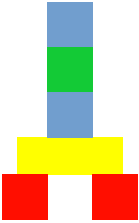
\includegraphics[scale=0.20]{figures/chapter2/task_goal.pdf}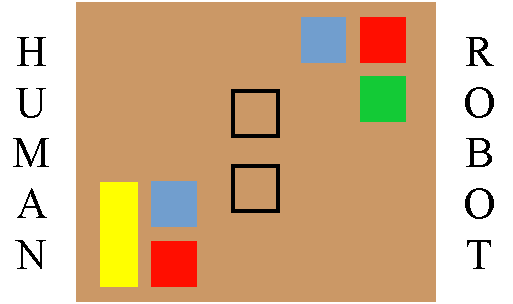
\includegraphics[scale=0.18]{figures/chapter2/task_setup_mini.pdf}}   
	\fancyhead[RO]{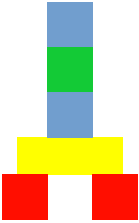
\includegraphics[scale=0.20]{figures/chapter2/task_goal.pdf}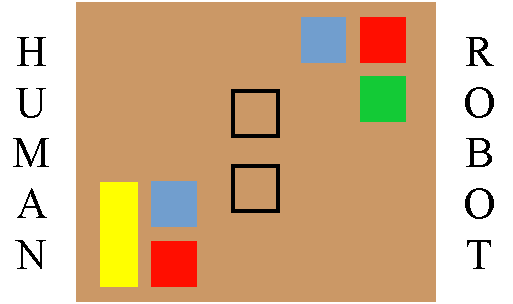
\includegraphics[scale=0.18]{figures/chapter2/task_setup_mini.pdf}\bfseries\thepage}  
	\fancyhead[RE]{\bfseries\nouppercase{\leftmark}}      % Chapter in the right on even pages
	\fancyhead[LO]{\bfseries\nouppercase{\rightmark}}     % Section in the left on odd pages
}%

\usepackage{pdfpages}
\usepackage{makecell}
\usepackage{pdflscape} 
\usepackage{mathtools}
\usepackage[section]{placeins}
\usepackage{afterpage}

%%%%%%%% my commands
\newcommand{\etal}{\textit{et al}.}
\newcommand{\ie}{\textit{i.e.}, }
\newcommand{\eg}{\textit{e.g.}, }
\newcommand{\fact}[3]{\mbox{\textit{#1}(#2, #3)}}
\newcommand{\circledtext}[1]{\raisebox{.5pt}{\textcircled{\raisebox{-.9pt} {#1}}}}
\newcommand{\sparql}{\textsc{SPARQL}}

\newcommand{\algConst}[1]{${\scriptscriptstyle #1}$}
\newcommand{\algNormTextSub}[2]{$\text{#1}_{#2}$}

\newcommand{\aslnumber}[1]{$#1$}
\newcommand{\aslstring}[1]{\textsf{#1}}
\newcommand{\aslvar}[1]{\textcolor{purple}{\textit{#1}}}
\newcommand{\asllabel}[1]{\textbf{#1}}
\newcommand{\annotation}[1]{{\footnotesize #1}}
\newcommand{\rulebody}[1]{\mbox{\hspace{.05\linewidth}}\begin{minipage}[t]{0.9\linewidth}#1.\end{minipage}}
\newcommand{\context}[1]{\begin{minipage}[t]{0.9\linewidth}#1\end{minipage}}
\newcommand{\planbody}[1]{\begin{minipage}[t]{0.9\linewidth}#1.\end{minipage}}
\newcommand{\Jason}[0]{\textbf{\textit{Jason}}}
\newcommand{\sn}{\mbox{\large\textbf{\texttt{\textasciitilde}}}}


\sloppy
\begin{document}
	\setcounter{chapter}{3} %% Numéro du chapitre précédent ;)
	\dominitoc
	\faketableofcontents
	\fi
	
	
\chapter{The central and pivotal role of Supervision}\label{chapter:chap4}
\minitoc
\section{State of the art}\label{chap4:subsec:state_art_sup}
The supervision component is the binder of a robotic architecture. Without it, there is no task, no interaction happening, it controls the other components of the architecture. Indeed, what we define by `supervision', in the context of \acrshort{hri}, is the higher level of the architecture, the process involving real-time decision-making, eventually based on plans, and action execution and monitoring. When speaking about joint action, we think it is the component that should handle coordination, communication, monitoring, repair strategies and eventually joint attention and common ground alignment, based on shared representations.

We can find in the literature multiple work proposing components with a part of these features. The ones that we will present have been a source of inspiration, from far or close, for the contributions of this thesis. We will start with the oldest one, Shary, which has been developed in our laboratory. It is a component dedicated to supervision for human-robot interactions, with a strong emphasis on communication, allowing to execute shared plans and to monitor human and robot actions~\cite{clodic_2009_shary}. Chaski is a task-level executor, focusing on coordination and decision-making. It takes as input shared plans with deadlines and minimize the human idle time when executing of this plans~\cite{shah_2011_improved}. There is also Pike an online executive that unifies intention recognition and plan adaptation to deal with temporal uncertainties during Shared Plan execution~\cite{karpas_2015_robust}. G\"{o}r\"{u}r and colleagues developed a robot able to handle unexpected human behavior, the first one being the human doing an action irrelevant to the task and the second one being the human not wanted the robot assistance~\cite{gorur_2017_toward, gorur_2018_social}. For this, they developed a human model and have a monitoring of human's actions and endow the robot with the abilities to be reactive and proactive. Similarly, Baraglia \etal{} proposed a reactive and proactive robot, being able to help when requested by the human or when detected~\cite{baraglia_2017_efficient}. Iocchi \etal{} presented a framework which generate and execute robust plans for service robots~\cite{iocchi_2016_practical}. It allows to not explicitly represent all possible situations would face (\eg low battery means the robot should not navigate) and also to face unpredicted situations where an action failed with no alternative solutions. They implemented it by separating the state variables needed at both planning and execution and the one needed at execution time only. Finally, Devin \etal{} implemented a supervisor allowing the robot to estimate the human's mental state about the environment and the states of the goals, plans and actions, while executing shared plans~\cite{devin_2016_implemented}.



\section{The Needs and Wants of a supervision system to manage interaction} % Requirements

%\section{Design Methodology}

A part of the control features presented here is inspired from Sandra Devin~\cite{devin_2017_decisional}. Indeed, we intended to pursue her work, re-implementing a part of her software using Jason, a BDI framework presented in Section~\ref{chap4:sec:bdi}, instead of if/else statements in C++, giving our software more flexibility, readability and genericity.
Then, to go further, we developed \acrfull{jahrvis}\footnote{Also almost the acronym for ``Just A Rather Very Intelligent System'', see \url{https://en.wikipedia.org/wiki/J.A.R.V.I.S.}}, a more complete approach of a supervision component dedicated to HRI which tries to satisfy multiple requirements:

\begin{bulletList}
	\item \textbf{Be generic}. The objectives developed in the rest of list are to reach for most collaborative tasks. Thus, it seemed essential for us to develop a software not dedicated to a particular human-robot task but able to handle plans for varied tasks. 
	\item \textbf{Take into account the human partner}. In HRI, the human and the robot are partners. As seen in Section~\ref{chap1:sec:ja}, partners perform better when taking each other into account. Thus, by considering human abilities, perspective and mental states, the supervisor makes the robot a better partner for the human.
	\item \textbf{Leave decisions to the human}. In some cases, it is not useful, even counterproductive that the robot plans everything beforehand. Indeed, such elements such as the human action parameters, or who should execute a given action when it does not matter, or the order in which some actions should be executed, can be decided at execution time. Thus, we propose a supervisor handling two types of plan allowing to give latitude to human decisions and actions: conditional plans, and plans extending ``Agent X'' shared plans~\cite{devin_2017_decisions}.
	\item \textbf{Monitor human actions}. To monitor the plan progress, the robot should be able to monitor the human, \ie recognize their actions or be able to tell if they are idle.
	\item \textbf{Handle contingencies}. The robot has a shared plan, this is one thing, but to execute it and lead to the goal success is another one. Indeed, first, it is not sure that the human has exactly the same, and failures can happen. Therefore, sometimes not everything is like the robot had planned and the decision and execution manager has to tackle this. Thus, it should be able to handle a certain amount of contingencies.
	\item \textbf{Manage relevant communications}. As stated in Section~\ref{chap1:sec:comm}, communication is one of the key of collaboration. Therefore, it is important to endow the robot with the ability to manage relevant communication actions, verbal and non-verbal.
	\item \textbf{Consider the interaction outside collaborative tasks} A robot dedicated to collaborative tasks, in a real-life context, will interact with humans outside or between these tasks. We propose to consider this fact by defining what we called \textit{interaction sessions}. An interaction session gives a frame to the interaction and allows to take into account a number of facts from one task to another or from one session to another.
	\item \textbf{Adapt to the human experience, abilities or preferences}. Humans are all different, because of their experience, abilities or preferences among other things. A robot taking into account its previous interactions with a human (\eg behaving differently with a novel user or an experienced user) or adapting to their abilities (\eg some people cannot climb stairs, a robot guide can indicate the elevator instead) will improve the efficiency and the quality of the interaction, and the user's experience.
\end{bulletList}


\section{Which tool to implement supervision?}\label{chap4:sec:bdi}

In this section, we will present the framework we chose as base for our supervision software. First, we explain how we did this choice and then the internal mechanisms of the framework. The supervision component itself, \acrshort{jahrvis}, we will be presented in the next Chapters.

\subsection{The Choice of the Programming Framework}

% mettre un petit paragraphe pour citer 
% citer RAE (papier Survey de Malik et Felix sur les HTN pour la robotique) et PRS, CRAM (pas de mécanismes de décision en ligne, ni de reprise d'erreur), JASON? + aucun de ces systèmes ne font de l'interaction humain robot
% difficulté de la planification d'un côté et de l'exécution du plan de l'autre
% l'originalité de JAHRVIS c'est de faire une exécution pour l'humain et le robot (avec les beliefs etc)

Restart from scratch or base oneself work on an existing software? This is the question which has been studied at the beginning of this thesis work about the implementation of the supervision software. It was possible 
\begin{inlineEnumerate}
	\item to develop the wanted features using the code\footnote{\url{https://github.com/laas/supervisor}} of the previous PhD student working on the supervision, Sandra Devin,\label{chap4:list:sandra}
	\item to choose among existing software dedicated to decision and execution for Human-Robot Interaction,\label{chap4:list:soft_hri}
	\item to choose among existing software dedicated to decision and execution for robotic platforms, and\label{chap4:list:robot}
	\item to develop a new software from scratch.\label{chap4:list:new}
\end{inlineEnumerate}

The obvious drawback of \ref{chap4:list:new} is that it takes a lot of time to start a new software from scratch and that it often leads to reinvent the wheel. Then, first we looked at existing solutions. Concerning the possibility \ref{chap4:list:sandra}, Devin had developed interesting features but the code is not modular and it was difficult to add new features or to modify the existing ones without breaking everything. Thus, there was the solutions \ref{chap4:list:soft_hri} and \ref{chap4:list:robot} left. When looking for existing software to manage human-robot interactions, we could not find any open-source one with a minimum of features, documentation and not entirely dedicated to a given task. Therefore, we turned ourselves toward robotic framework. We compared existing open-source decision-making and execution software for robots. To cite a few, there is the PetriNetPlans library introduced by Ziparo \etal~\cite{ziparo_2011_petri} which is a framework for planning and execution. Beetz \etal{} developed CRAM, a software implementing reasoning mechanisms that can infer control decisions~\cite{beetz_2010_cram}. A framework to implement hierarchical state machines is available among ROS libraries, SMACH\footnote{\url{http://wiki.ros.org/smach}}, defined as ``task-level architecture for rapidly creating complex robot behavior''. Or, a C++ library to create behavior trees has been developed, called BehaviorTree.CPP~\footnote{\url{https://github.com/BehaviorTree/BehaviorTree.CPP/}}. Finally, there are several implementations of the BDI model presented in Section~\ref{chap3:sec:archi} such as JAM~\cite{huber_1999_jam}, Jadex~\cite{braudach_2005_jadex}, SPARK~\cite{morley_2004_spark}, dMARS~\cite{dinverno_1998_formal}, OpenPRS~\cite{ingrand_1996_prs} or Jason~\cite{bordini_2007_jason}. 

As a first step, for prototyping and respecting project deadlines, our choice went to SMACH because its compatibility with ROS and its facility to be used. Then, it was no surprise, it became more and more difficult to program complex robot behaviors, state machine were not enough powerful. Thus, we examined possibilities for our second choice. After a comparison considering potential compatibility with ROS, possible integration with the other software of our architecture, availability of documentation, users' feedbacks, maintenance, and possibility of code modifications, our choice went to Jason designed by Bordini \etal~\cite{bordini_2007_jason} which is a Java interpreter of AgentSpeak created by Rao~\cite{rao_1996_agentspeak}. It has the advantage to be a BDI (Beliefs, Desires, Intentions, see Section~\ref{chap3:sec:archi}) agent-oriented framework, fitting with our architecture. BDI framework implement a process, called the reasoning cycle or more commonly the sense-decide-act cycle~\cite{albus_1991_outline}, deciding step by step, which action to perform to reach a goal. It allows more modularity than state machines to handle contingencies and events. It also facilitates reasoning on agents' -- humans and robot -- beliefs. We chose this framework among the BDI ones and not another because it is implemented in Java and thus was compatible with rosjava\footnote{\url{https://github.com/rosjava/rosjava_core}} (\ie ROS implementation in Java), it is still developed and maintained, it is well documented (theoretically~\cite{bordini_2007_jason} and implement-ally\footnote{\url{http://jason.sourceforge.net/api/}}) which allows source code understanding and modifications, and there is a mailing list for users and its archives available\footnote{\url{https://sourceforge.net/p/jason/mailman/jason-users/}}.

\subsection{Programming with Jason}\label{chap4:subsec:jason}
As said above, Jason is a BDI-based framework, allowing what is called \textit{agent-oriented programming}. Originally designed for multi-robot programming, it can be used for other purposes such as ours. How does it work?

We explained in Section~\ref{chap3:sec:archi} that there were three main concepts involved in BDI models: beliefs, desires and intentions. Well, Jason's purpose is to program agents. Thus, each agent has beliefs, desires and intentions. The beliefs are what it perceives, acquires from other agents and computes. They can produce desires, \ie states of affairs the agent wants to achieve. Then, the agent deliberates on its desires and choose to commit to some of them, \ie the chosen desires become intentions. To satisfy its intentions, the agent executes procedural programs, called plans, leading to actions. The procedural knowledge is written by the programmer.

The programming of the behavior of an agent is in the AgentSpeakLanguage (ASL). The program is designed by a user, a programmer. A program contains, among other things, plans. These plans have actions. An action is described by a Java program, written by the Jason's user. Then, to run, a program uses the decision loop, so called the \textit{reasoning cycle}, integrated to Jason. It is possible to customize some functions of the reasoning cycle by overloading or adding Java functions of the agent's constructors, belief base and reasoning cycle. 

\subsubsection{Agents} In the ASL program of an agent, it is possible to see plans, beliefs, desire and test goal. First, let's see a very simple example of program with the agent Bob\footnote{\url{http://jason.sourceforge.net/mini-tutorial/hello-bdi/}}, presented in Listing~\ref{chap4:lst:bob}. Bob has one initial (\ie given by the programmer, not acquired by perception) belief which is |happy(bob)|. A belief is a property, here |happy|, which can have whatever number of arguments (including zero), here |bob| and a source (\eg |source(percept)| means that the belief has been acquired through perception, |source(self)| means that it has been computed by the agent itself and |source(alice)| means that it has been received from the agent Alice). Then, he has one initial desire which is recognizable by |!|. And finally, he has a plan allowing to achieve the desire |say(hello)|. A plan is triggered by an event, here |+!say(X)| (\ie the event is that the goal |say(hello)| has been added), has a context (\ie a precondition), here |happy(bob)| and has a body which contains the actions to execute, here |.print(X)| (with |X| being a variable -- variables have their first letter in upper case). If we remove the initial belief |happy(bob)| from the first line, as the program is written and considering that Bob is the only agent, he cannot print hello, as the precondition of the plan will not be true.

\begin{lstlisting}[caption={ASL program of Bob, a Jason agent}, label={chap4:lst:bob}]
happy(bob).	\\belief

!say(hello).	\\desire

\\plan
+!say(X) : happy(bob) <- 
	.print(X).		
\end{lstlisting} 

In another example, illustrated by Listing~\ref{chap4:lst:bobalice}, Bob has no initial belief nor initial goal. He has plans for two events: starting to believe he is happy and having the goal to say hello. We can see that there is also a program for another agent, Alice. She has an initial goal, her, which is to inform bob that he is happy. Therefore, we can see that an agent can add a belief in another agent's belief base. When Bob gets the information that he is happy, this triggers his first plan, creating for him the goal |!say(hello)|. As Bob does not believe that today is Monday, he can trigger his second plan to say hello. In this plan, there a three elements: a print action, a wait action and the addition of a new goal. And thus, here, we are in the presence of a recursive plan which never ends. 

\begin{lstlisting}[caption={ASL programs of Bob and Alice, two Jason agent}, label={chap4:lst:bobalice}]
\\bob.asl
\\for example purposes, the precondition is true
\\but it can be logical expressions with beliefs,
\\functions...
+happy(bob) : true <- 
	!say(hello).

+!say(X) : not today(monday) <- 
	.print(X); 
	.wait(500); 
	!say(X).

\\alice.asl
!inform.

+!inform : true <- .send(bob,tell,happy(bob)).
\end{lstlisting} 

\subsubsection{Actions} To give an idea of what looks like the Java program of an action, here is an example of a Java function for the action |.print| in Listing~\ref{chap4:lst:print}.

\begin{lstlisting}[caption={.print action}, label={chap4:lst:print}, language=Java]
public class print extends DefaultInternalAction {
	@Override
	public Object execute(TransitionSystem ts, Unifier un, Term[] args) throws Exception {
		String sout = argsToString(args);
		System.out.print(sout.toString() + "\n");
	}
	return true;
	}
}
\end{lstlisting} 

In Jason, there are two types of actions defined: \emph{environment actions} and \emph{internal actions}. \emph{Environment actions} allow an agent to act within its environment, usually producing effects visible by other agents. Whereas, \emph{internal actions} are designed to be run internally within an agent such as the print action and can be used to return values or booleans. When being executed, there are not handled the same way in the Jason's reasoning cycle. The definition of which type an action should be falls to the programmer, which should choose according to their need.

We have seen what looks like the program of Jason agent. Now, we are going to see how it is run by the Jason interpreter.


\subsubsection{Reasoning cycle} Each agent has what has been coined a \textit{reasoning cycle}, composed of 10 steps. It resembles a decision loop, running each step one by one and starting again at the first one. The steps 1 to 4 are dedicated to the belief update of the agent. The steps 5 to 10 describe the interpretation of the ASL program. In these latter, an event is selected, as well as a plan corresponding to this event and then the first formula (\eg an action or a goal) of the plan is executed. It is illustrated by Figure~\ref{chap4:fig:jason_cycle}. The steps are the following ones, in this order:
\begin{enumerate}
	\item Perceiving the Environment: Each agent has a Java function called |perceive|. This function can retrieve data from a simulated environment or be customized by the programmer to get actual perception data. The function outputs a list of beliefs, along with their source (\eg |<isOn(box1,table)[source(percept)]|, |color(box1,red)[source(percept)]>|).
	\item Updating the Belief Base: The agent's belief base is updated with the perception data. Each change in the belief base generates an event (\eg |+color(box1,red)[source(percept)]| and if later the color of the box is not part of the perception data anymore, it will be |-color(box1,red)[source(percept)]|).\label{chap4:list:update_bb}
	\item Receiving Communication from Other Agents: It checks if an agent received a message from another agent such as the message Bob received from Alice in Listing~\ref{chap4:lst:bobalice}. A message can be a belief, a plan, a goal or a questioning on a given belief.
	\item Selecting ‘Socially Acceptable’ Messages: It is a function the programmer should customize. It allows agent to refuse messages or types of message from some given agents based on some rules written in Java by the programmer, \eg no message from the agent Alice.
	\item Selecting an Event: Events are either perceived changes in the environment or changes in the agent's own goals. There is a queue of events and at each reasoning cycle only one is selected to be handled. The default method to select it is a FIFO but, as every function of the reasoning cycle, it can be customized. 
	\item Retrieving all Relevant Plans: From the selected event, it tries to find all the relevant plans for this event, in the plan library, \ie the plans written by the programmer in ASL. The function tries to find the plans that can be \textit{unified} with event, \ie the ones with their left part (the trigger) matching the event. For example, if the selected event is |+color(box1,red)[source(percept)]| and in the plan library there are these six plans:
\begin{lstlisting}[style=inline]
+position(Object,Coords) : true <- .print(Coords).
+color(Object,red) : true <- .print(nice).
+color(Object,red)[source(self)] : true <- .print(nice).
+color(box1,Color) : true <- .print(nice).
+color(Object,Color) : false <- .print(Color).
+color(Object,blue) : true <- .print(so-so).
\end{lstlisting}
	then there are three relevant plans (the last one is also relevant because what is looked for here is the triggers only and not the preconditions):
\begin{lstlisting}[style=inline]
+color(Object,red) : true <- .print(nice).
+color(box1,Color) : true <- .print(nice).
+color(Object,Colour) : false <- .print(Colour).
\end{lstlisting}
	\item Determining the Applicable Plans: It takes the list of relevant plans and sees which ones are applicable. To do so, it looks at the context (the preconditions) of the plans. The context can be beliefs, prolog-like rules, internal actions, logical expressions or booleans. If we look at the example of the previous step, there were three relevant plans. Their contexts are simple booleans. Two of them are true, the other one is false, thus the two first plans are applicable.
	\item Selecting One Applicable Plan: It takes the list of applicable plans and selects the one that will be elected to become an intention, \ie to be executed. As usual, this is a customizable function for which the default behavior is to take the first plan in the order of the plan library, \ie in the order written by the programmer. Still with the same example, thus, the one plan to be selected is the first one, |+color(Object,red) : true <- .print(nice).| If the event was external, \ie from perception, it creates a new intention, adding it to the set of intentions. Then, the agent has a new \textit{focus of attention}. If the event was internal, \eg a belief addition inside a plan, then the selected plan is added on the top of the existing intention. 
	\item Selecting an Intention for Further Execution: As seen in the previous step, an agent can have more than one intention in the set of intentions, each representing a different focus of attention. Then, at this step is chosen the intention of which the formula will be executed. The default function chooses the first intention of the list. After execution of the formula, the intention will go at the end of the intentions list.
	\item Executing One Step of an Intention: The first formula of the selected intention is executed (this number is also customizable and the programmer can choose that an agent execute more than once formula in the same reasoning cycle). It can be an internal action, an environment action, a goal, a belief addition or deletion and two other types that will not be developed here. 
\end{enumerate}

Therefore, each agent has a reasoning cycle running repeatedly, independent from the other agents' reasoning cycle. Interactions between each agents happen through the messages they send to each others and eventually the effects they produce on the environment which are then perceived by the other agents. 


\begin{landscape}
\begin{figure}
	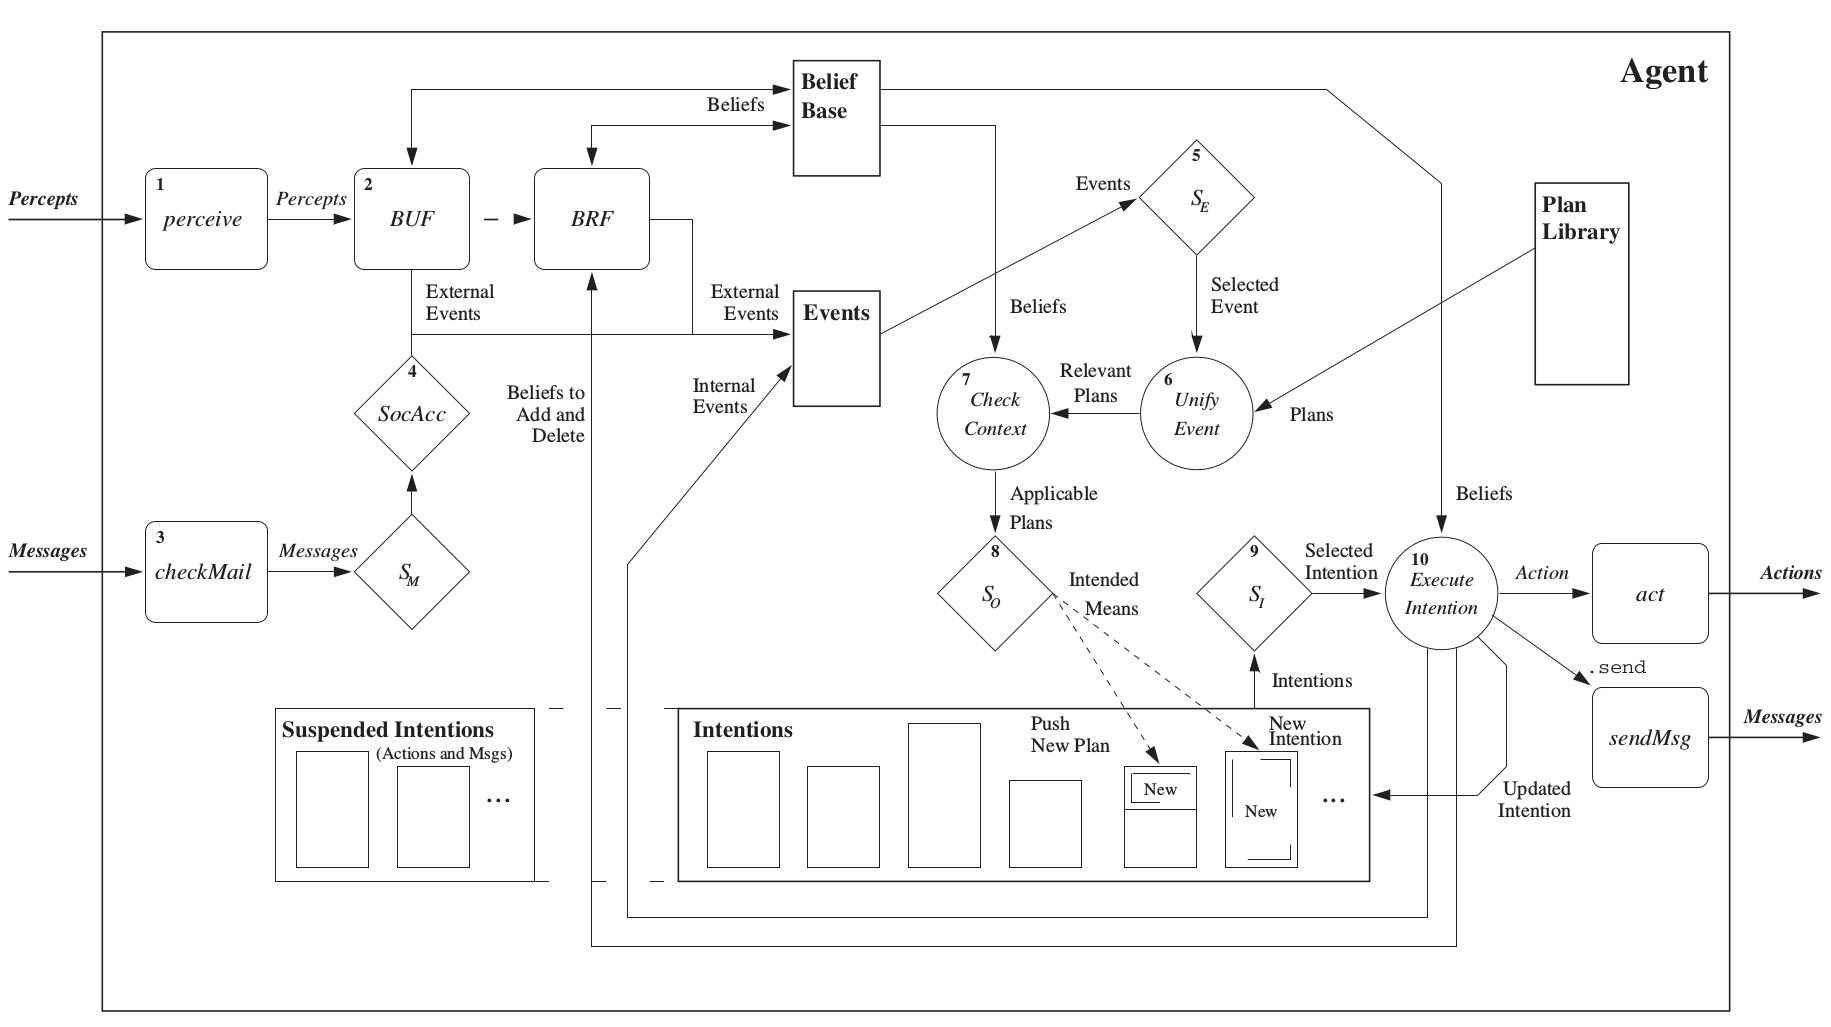
\includegraphics[width=\linewidth]{figures/chapter2/jason_cycle.png}
	\caption{The Jason reasoning cycle~\cite{bordini_2007_jason}. Each step presented above has its numbered corresponding box.}
	\label{chap4:fig:jason_cycle}
\end{figure}
\end{landscape}

\subsubsection{Plan failure handling}

For the case where a plan fails (\eg an action fails -- there are other reasons for which a plan could fail but we will not discuss the details here), Jason integrates a mechanism handling failures. It consists in cancel the execution of the plan and generating a triggering event for a contingency plan whose prefix is |-!|. If the contingency plan can be found -- written by the programmer --, it is executed. Then, if the plan which originally failed was a subplan of another plan, this plan will continue normally. 

An illustration is given in Listing~\ref{chap4:lst:failure}. The result of the execution of this agent file would be the printing ``unknown error'' and then ``bye'' in case of the failure of the |robot_speech| action execution with an instantiated speech module. Indeed, the initial goal |speak| creates the subgoal |say_hello|. Unfortunately, the action |robot_speech| fails with an empty error message, generating the event |-!say_hello[error_msg(Msg)]|. There are two plans for this event but as |Msg=""|, the second one is chosen, printing ``unknown error''. Then, |speak| continues in the same way it does when goal |say_hello| is achieved successfully, printing ``bye''.

\begin{lstlisting}[caption={Example of plan failure handling}, label={chap4:lst:failure}]
!speak.

+!speak : true <- 
!say_hello;
.print(bye).

+!say_hello : true <-
robot_speech(hello);
.print(hello).

-!say_hello[error_msg(Msg)] : .substring(Msg,no_speech_found) <-
.print(no speech module was found).

-!say_hello[error_msg(Msg)] : true <-
.print(unknown error).	
\end{lstlisting} 

\subsection{Jason Integration with ROS}
The robotic architecture presented in Section~\ref{chap3:sec:rob_archi} uses the ROS framework~\cite{quigley_2009_ros} to enable communication between its components. Thus, to be able to build a supervision software based on Jason, we needed to interface it with ROS as well. At the time, there was no available bridge between Jason and ROS, Jason being extensively used in simulation contexts. Thus, we developed our own -- and at about the same moment, the Jason's developers started to develop theirs~\cite{silva_2020_embedded} (what we realized a bit later), both using rosjava. We tackled the problem in very different ways. A user of their implementation only needs to fill one perception (topics) and one action (topics/services) manifests to link the system with ROS and then implement their agent in ASL. Thus, it is quite easy to use. However, it has drawbacks. Therefore, action requests are directly sent from ASL to the hardware controller, with no possibility of Java processing. Moreover, action status/result can only be boolean which is not enough for a system like ours needing to perform service queries of data to the external Knowledge Base for example. Finally, there is no bridge with action servers which are often used for motion planers for example. 

\begin{figure}[!ht]
	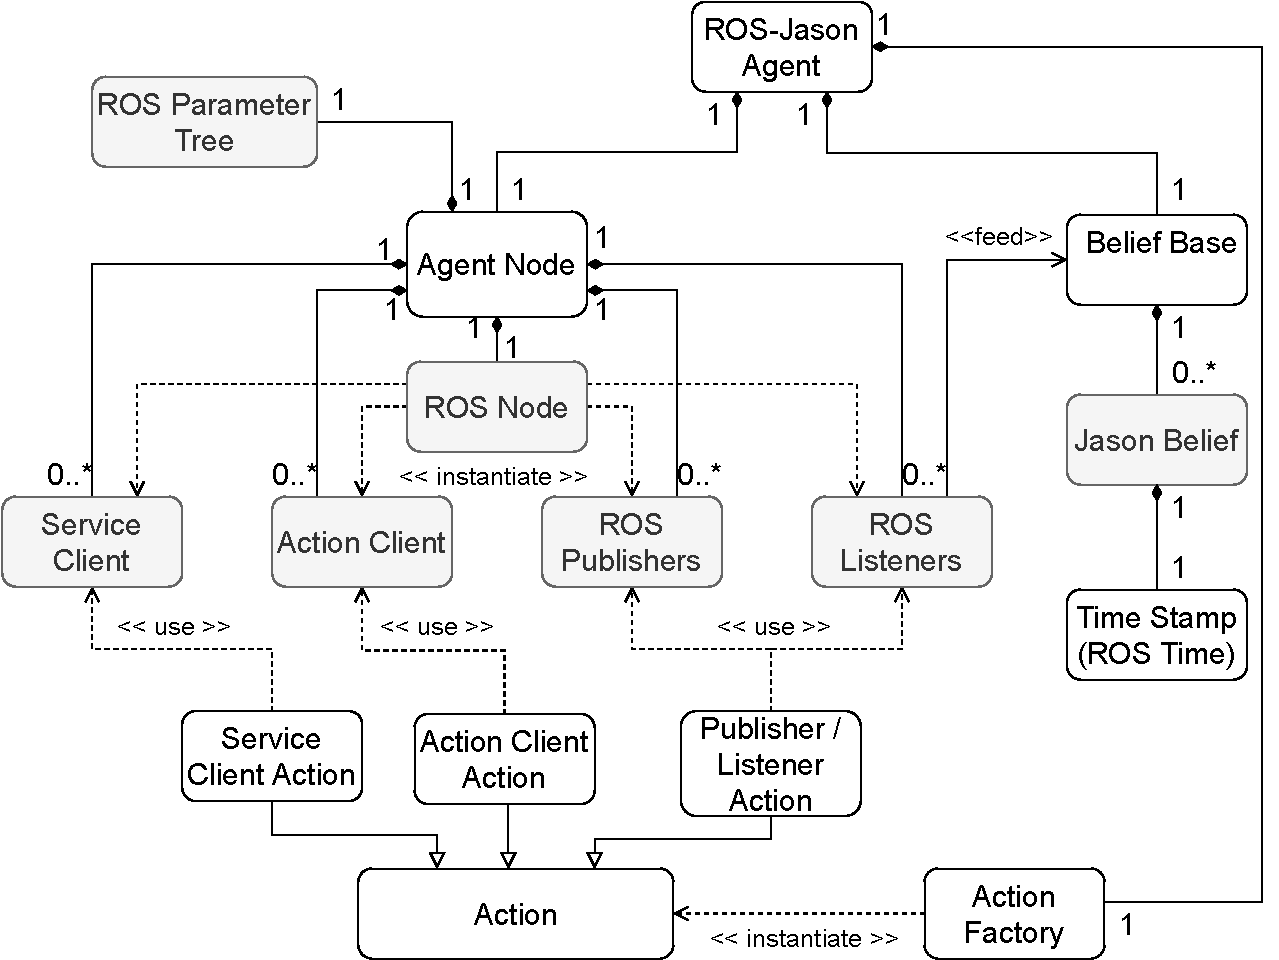
\includegraphics[width=\linewidth]{figures/chapter2/RJS_diagram.pdf}
	\caption{Simplified Java class diagram of our ROS-Jason implementation. In white are our customized classes and in grey the native ROS and Jason classes.}
	\label{chap4:fig:rjs}
\end{figure}

A simplified Java class diagram of our  implementation\footnote{\url{https://github.com/amdia/rjs}} is presented in Figure~\ref{chap4:fig:rjs}. We defined for each Jason agent a customized Java class (\acrfull{rja} on the figure) which has an Agent Node, an action factory and a belief base where all beliefs are time stamped with the roscore time. 

An Agent Node has an attribute, the ROS Parameter Tree, allowing to load YAML parameters from files in which, among other things, are written services, topics and action servers info, as shown in Listing~\ref{chap4:lst:ros-jason}, a bit similarly to the manifests of~\cite{silva_2020_embedded}. From these parameters, the Agent Node can automatically instantiate all the needed ROS components through its ROS node. 

\bigskip

An \acrshort{rja} can receive perception updates in its Belief Base through ROS topic listeners. Moreover, we customized\footnote{This modification of the belief update function is not part of our ROS-Jason implementation but is on top of it, in the \acrshort{jahrvis} implementation which relies on ROS-Jason.} the belief update function (step~\ref{chap4:list:update_bb} of the reasoning cycle) as we chose to abandon a state-based perception to adopt an event-based perception. So, percepts are not elements that when perceived at time T are added to the belief base and disappearing when not perceived anymore at time T+1. There are now updates (additions and deletions) from the external Knowledge Base, in this way, it limits the number of message exchanges, \ie instead of receiving every 500 ms during 10 seconds that the agent perceives |cube_1|, it receives for example an addition at t=18s and a deletion at t=28s. 

To each belief added in the belief base, from perception or internal computation, is added a time stamp from the current ROS time. Currently, it is useful for the computation of the Quality of Interaction presented in Chapter~\ref{chapter:chap7} and also to feed the \acrshort{kb} timeline and for debugging.

An \acrshort{rja} has an Action Factory -- abstract in the ROS-Jason framework and instantiated in \acrshort{jahrvis} -- containing the list of environment actions it can perform -- in the case of our architecture, not all actions of this type are for the robot to act on its environment, sometimes there are queries to other components of the architecture. The Action Factory instantiates the Action called through the ASL program at execution time. An Action can either be based on a ROS service client, or an ROS action client, or a ROS publisher for the request and a ROS listener for the result. 

\begin{lstlisting}[caption={Example of service, topic and action server definitions in a YAML file.}, label={chap4:lst:ros-jason}]
services:
	onto_individual: 
		name: /ontologenius/individual/robot
		type: ontologenius/OntologeniusService
	onto_class: 
		name: /ontologenius/class/robot
		type: ontologenius/OntologeniusService
topics:
	mementar_occasions: 
		name: /mementar/occasions/robot
		type: mementar/MementarOccasion
		function: sub
	plan_request:
		name: /planner/request_new_plan
		type: planner_msgs/PlanRequest
		function: pub
action_servers:
	plan_motion: /pr2_tasks_node/plan
	execute_motion: /pr2_tasks_node/execute
\end{lstlisting}

\ifdefined\included
\else
\bibliographystyle{acm}
\bibliography{These}
\end{document}
\fi

\part{Joint Action-based Human-Aware supeRVISor: \acrshort{jahrvis}}\label{part:part3}
\begin{partintro}
	We presented in Section~\ref{chap4:subsec:state_art_sup} a few work tackling supervision issues, \ie how to adapt to the human, how to monitor them, how to face unexpected human behavior, how to optimize the task efficiency, how to make the robot a good human helper... They were very inspiring but we found out it was missing a general architecture and a software that could be used in different types of collaborative tasks, available for the community and that could easily be enhanced with new features. These thoughts led to the development of the \acrfull{jahrvis} which is the central topic of this part. We also came up with a novel idea: to endow the robot with the ability to measure if an interaction is going well or not. Such ability can be used by the supervision to enhance its adaptation capacity.
\end{partintro}

\ifdefined\included
\else
\documentclass[a4paper,11pt,twoside]{StyleThese}
\usepackage{amsmath,amssymb, amsthm}             % AMS Math
\usepackage[T1]{fontenc}
\usepackage[utf8x]{inputenc}
\usepackage{babel}
\usepackage{datetime}

\usepackage{silence}

\WarningFilter{minitoc(hints)}{W0023}
\WarningFilter{minitoc(hints)}{W0028}
\WarningFilter{minitoc(hints)}{W0030}

\usepackage{lmodern}
\usepackage{tabularx}
%\usepackage{tabular}
\usepackage{multirow}
\usepackage{xspace}

\usepackage{subfig}
\usepackage[inline]{enumitem}

\usepackage{hhline}
\usepackage[left=1.5in,right=1.3in,top=1.1in,bottom=1.1in,includefoot,includehead,headheight=13.6pt]{geometry}
\renewcommand{\baselinestretch}{1.05}

% Table of contents for each chapter

\usepackage[nottoc, notlof, notlot]{tocbibind}
\usepackage{minitoc}
\setcounter{minitocdepth}{2}
\mtcindent=15pt
% Use \minitoc where to put a table of contents

\usepackage{aecompl}

% Glossary / list of abbreviations

\usepackage[intoc]{nomencl}
\iftoggle{ThesisInEnglish}{%
\renewcommand{\nomname}{Glossary}
}{ %
\renewcommand{\nomname}{Liste des Abréviations}
}

\usepackage{etoolbox}
\renewcommand\nomgroup[1]{%
  \item[\bfseries
  \ifstrequal{#1}{A}{Number Sets}{%
  \ifstrequal{#1}{G}{Agents Beliefs and Action Models}{%
  \ifstrequal{#1}{N}{Navigation}{%
  \ifstrequal{#1}{O}{Ontology}{%
  \ifstrequal{#1}{R}{Referring Expression Generation}{%
  \ifstrequal{#1}{Z}{Controllable and Uncontrollable Agents Task Planning}{}}}}}}%
]}

\makenomenclature



% My pdf code

\usepackage{ifpdf}

\ifpdf
  \usepackage[pdftex]{graphicx}
  \DeclareGraphicsExtensions{.jpg}
  \usepackage[pagebackref,hyperindex=true]{hyperref}
  \usepackage{tikz}
  \usetikzlibrary{arrows,shapes,calc}
\else
  \usepackage{graphicx}
  \DeclareGraphicsExtensions{.ps,.eps}
  \usepackage[dvipdfm,pagebackref,hyperindex=true]{hyperref}
\fi

\graphicspath{{.}{images/}}

%% nicer backref links. NOTE: The flag ThesisInEnglish is used to define the
% language in the back references. Read more about it in These.tex

\iftoggle{ThesisInEnglish}{%
\renewcommand*{\backref}[1]{}
\renewcommand*{\backrefalt}[4]{%
\ifcase #1 %
(Not cited.)%
\or
(Cited in page~#2.)%
\else
(Cited in pages~#2.)%
\fi}
\renewcommand*{\backrefsep}{, }
\renewcommand*{\backreftwosep}{ and~}
\renewcommand*{\backreflastsep}{ and~}
}{%
\renewcommand*{\backref}[1]{}
\renewcommand*{\backrefalt}[4]{%
\ifcase #1 %
(Non cité.)%
\or
(Cité en page~#2.)%
\else
(Cité en pages~#2.)%
\fi}
\renewcommand*{\backrefsep}{, }
\renewcommand*{\backreftwosep}{ et~}
\renewcommand*{\backreflastsep}{ et~}
}

% Links in pdf
\usepackage{color}
\definecolor{linkcol}{rgb}{0,0,0.4} 
\definecolor{citecol}{rgb}{0.5,0,0} 
\definecolor{linkcol}{rgb}{0,0,0} 
\definecolor{citecol}{rgb}{0,0,0}
% Change this to change the informations included in the pdf file

\hypersetup
{
bookmarksopen=true,
pdftitle="Endowing the robot with the abilities to control and evaluate its contribution to a human-robot joint action",
pdfauthor="Amandine MAYIMA", %auteur du document
pdfsubject="Thèse", %sujet du document
%pdftoolbar=false, %barre d'outils non visible
pdfmenubar=true, %barre de menu visible
pdfhighlight=/O, %effet d'un clic sur un lien hypertexte
colorlinks=true, %couleurs sur les liens hypertextes
pdfpagemode=None, %aucun mode de page
pdfpagelayout=SinglePage, %ouverture en simple page
pdffitwindow=true, %pages ouvertes entierement dans toute la fenetre
linkcolor=linkcol, %couleur des liens hypertextes internes
citecolor=citecol, %couleur des liens pour les citations
urlcolor=linkcol %couleur des liens pour les url
}

% definitions.
% -------------------

\setcounter{secnumdepth}{3}
\setcounter{tocdepth}{2}

% Some useful commands and shortcut for maths:  partial derivative and stuff

\newcommand{\pd}[2]{\frac{\partial #1}{\partial #2}}
\def\abs{\operatorname{abs}}
\def\argmax{\operatornamewithlimits{arg\,max}}
\def\argmin{\operatornamewithlimits{arg\,min}}
\def\diag{\operatorname{Diag}}
\newcommand{\eqRef}[1]{(\ref{#1})}

\usepackage{rotating}                    % Sideways of figures & tables
%\usepackage{bibunits}
%\usepackage[sectionbib]{chapterbib}          % Cross-reference package (Natural BiB)
%\usepackage{natbib}                  % Put References at the end of each chapter
                                         % Do not put 'sectionbib' option here.
                                         % Sectionbib option in 'natbib' will do.
\usepackage{fancyhdr}                    % Fancy Header and Footer

% \usepackage{txfonts}                     % Public Times New Roman text & math font
  
%%% Fancy Header %%%%%%%%%%%%%%%%%%%%%%%%%%%%%%%%%%%%%%%%%%%%%%%%%%%%%%%%%%%%%%%%%%
% Fancy Header Style Options

\pagestyle{fancy}                       % Sets fancy header and footer
\fancyfoot{}                            % Delete current footer settings

%\renewcommand{\chaptermark}[1]{         % Lower Case Chapter marker style
%  \markboth{\chaptername\ \thechapter.\ #1}}{}} %

%\renewcommand{\sectionmark}[1]{         % Lower case Section marker style
%  \markright{\thesection.\ #1}}         %

\fancyhead[LE,RO]{\bfseries\thepage}    % Page number (boldface) in left on even
% pages and right on odd pages
\fancyhead[RE]{\bfseries\nouppercase{\leftmark}}      % Chapter in the right on even pages
\fancyhead[LO]{\bfseries\nouppercase{\rightmark}}     % Section in the left on odd pages

\let\headruleORIG\headrule
\renewcommand{\headrule}{\color{black} \headruleORIG}
\renewcommand{\headrulewidth}{1.0pt}
\usepackage{colortbl}
\arrayrulecolor{black}

\fancypagestyle{plain}{
  \fancyhead{}
  \fancyfoot{}
  \renewcommand{\headrulewidth}{0pt}
}

%\usepackage{MyAlgorithm}
%\usepackage[noend]{MyAlgorithmic}
\usepackage{algorithm}
\usepackage[noend]{algpseudocode}
\usepackage{comment}
\usepackage[ED=MITT-InfoTel, Ets=INSA]{tlsflyleaf}
%%% Clear Header %%%%%%%%%%%%%%%%%%%%%%%%%%%%%%%%%%%%%%%%%%%%%%%%%%%%%%%%%%%%%%%%%%
% Clear Header Style on the Last Empty Odd pages
\makeatletter

\def\cleardoublepage{\clearpage\if@twoside \ifodd\c@page\else%
  \hbox{}%
  \thispagestyle{empty}%              % Empty header styles
  \newpage%
  \if@twocolumn\hbox{}\newpage\fi\fi\fi}

\newcommand*{\algrule}[1][\algorithmicindent]{%
	\makebox[#1][l]{%
		\hspace*{.2em}% <------------- This is where the rule starts from
		\vrule height .75\baselineskip depth .25\baselineskip
	}
}

%%% to have lines in algorithm, from stackexchange
\newcount\ALG@printindent@tempcnta
\def\ALG@printindent{%
	\ifnum \theALG@nested>0% is there anything to print
	\ifx\ALG@text\ALG@x@notext% is this an end group without any text?
	% do nothing
	\else
	\unskip
	% draw a rule for each indent level
	\ALG@printindent@tempcnta=1
	\loop
	\algrule[\csname ALG@ind@\the\ALG@printindent@tempcnta\endcsname]%
	\advance \ALG@printindent@tempcnta 1
	\ifnum \ALG@printindent@tempcnta<\numexpr\theALG@nested+1\relax
	\repeat
	\fi
	\fi
}
% the following line injects our new indent handling code in place of the default spacing
\patchcmd{\ALG@doentity}{\noindent\hskip\ALG@tlm}{\ALG@printindent}{}{\errmessage{failed to patch}}
\patchcmd{\ALG@doentity}{\item[]\nointerlineskip}{}{}{} % no spurious vertical space
% end vertical rule patch for algorithmicx

\makeatother
 
%%%%%%%%%%%%%%%%%%%%%%%%%%%%%%%%%%%%%%%%%%%%%%%%%%%%%%%%%%%%%%%%%%%%%%%%%%%%%%% 
% Prints your review date and 'Draft Version' (From Josullvn, CS, CMU)
\newcommand{\reviewtimetoday}[2]{\special{!userdict begin
    /bop-hook{gsave 20 710 translate 45 rotate 0.8 setgray
      /Times-Roman findfont 12 scalefont setfont 0 0   moveto (#1) show
      0 -12 moveto (#2) show grestore}def end}}
% You can turn on or off this option.
% \reviewtimetoday{\today}{Draft Version}
%%%%%%%%%%%%%%%%%%%%%%%%%%%%%%%%%%%%%%%%%%%%%%%%%%%%%%%%%%%%%%%%%%%%%%%%%%%%%%% 

\newenvironment{maxime}[1]
{
\vspace*{0cm}
\hfill
\begin{minipage}{0.5\textwidth}%
%\rule[0.5ex]{\textwidth}{0.1mm}\\%
\hrulefill $\:$ {\bf #1}\\
%\vspace*{-0.25cm}
\it 
}%
{%

\hrulefill
\vspace*{0.5cm}%
\end{minipage}
}

\let\minitocORIG\minitoc
\renewcommand{\minitoc}{\minitocORIG \vspace{1.5em}}

\usepackage{multirow}
%\usepackage{slashbox}

\newenvironment{bulletList}%
{ \begin{list}%
	{\tiny$\bullet$}%
	{\setlength{\labelwidth}{25pt}%
	 \setlength{\leftmargin}{30pt}%
	 \setlength{\itemsep}{-0.5em}}}%
{ \end{list} }

\newenvironment{inlineEnumerate}
{\begin{enumerate*} [label={(\arabic*)}] }
{\end{enumerate*}}

\theoremstyle{definition}
\newtheorem{definition}{Definition}
\renewcommand{\epsilon}{\varepsilon}

% centered page environment

\newenvironment{vcenterpage}
{\newpage\vspace*{\fill}\thispagestyle{empty}\renewcommand{\headrulewidth}{0pt}}
{\vspace*{\fill}}

\newenvironment{asl}{\ttfamily\begin{tabbing}~~~\=$\leftarrow$ \= ~~~ \=
		\kill}{\end{tabbing}}

\usepackage{tablefootnote}

\theoremstyle{plain}
\newtheorem{constraint}{Constraint}[section]

\algnewcommand\algorithmicforeach{\textbf{for each}}
\algnewcommand\algorithmicin{\textbf{in}}
\algdef{S}[FOR]{ForEach}[2]{\algorithmicforeach\ #1\ \algorithmicin\ #2\ \algorithmicdo}

\algnewcommand\algorithmicforkxor{\textbf{do fork-join-xor}}
\algnewcommand\algorithmicendforkxor{\textbf{end fork-join-xor}}
\algdef{SE}{ForkXor}{EndForkXor}{\algorithmicforkxor}{\algorithmicendforkxor}


\usepackage{listings}
\lstset{
	frame=single,
	captionpos=b,
	breaklines=true,
	basicstyle=\ttfamily,
	numberstyle=\color{black},
	tabsize=2,
	mathescape=true,
	literate=%
		{â}{{\^a}}1
}

\lstdefinestyle{inline}{
	frame=none,
	aboveskip=\smallskipamount,
	belowskip=\smallskipamount,
}

\lstdefinestyle{OwlTurtle}{
	language=C,
	tabsize=4,
	basicstyle=\scriptsize\ttfamily,
	keywordstyle=\bfseries\color{darkgray},
	morekeywords={rdf:type, rdfs:domain, rdfs:subPropertyOf, rdfs:range, :hasSubtask, :DecompositionUsedBy, rdfs:subClassOf, :hasDecomposition, owl:inverseOf, htn_actions:hasEffect, rdfs:label},
	alsoletter=:
}

\lstdefinestyle{aslDef}{
	frame=none,
%	breaklines=false,
	%xleftmargin=.1\textwidth, xrightmargin=.1\textwidth
}

\fancypagestyle{example}{%
	\fancyhead[LE]{\bfseries\thepage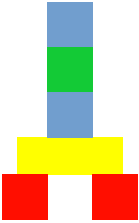
\includegraphics[scale=0.20]{figures/chapter2/task_goal.pdf}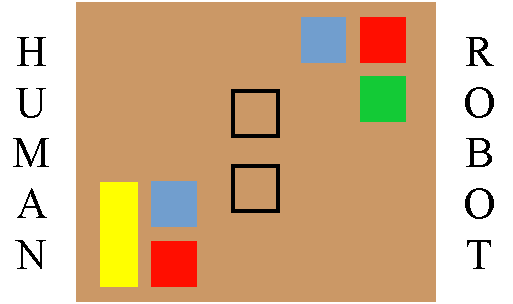
\includegraphics[scale=0.18]{figures/chapter2/task_setup_mini.pdf}}   
	\fancyhead[RO]{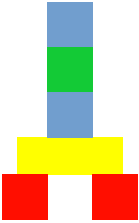
\includegraphics[scale=0.20]{figures/chapter2/task_goal.pdf}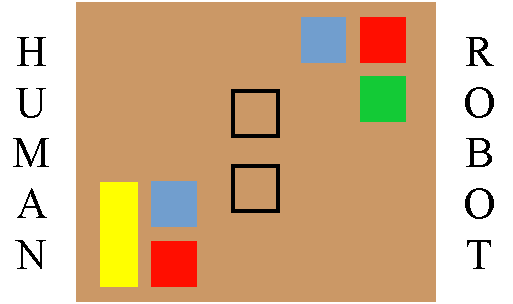
\includegraphics[scale=0.18]{figures/chapter2/task_setup_mini.pdf}\bfseries\thepage}  
	\fancyhead[RE]{\bfseries\nouppercase{\leftmark}}      % Chapter in the right on even pages
	\fancyhead[LO]{\bfseries\nouppercase{\rightmark}}     % Section in the left on odd pages
}%

\usepackage{pdfpages}
\usepackage{makecell}
\usepackage{pdflscape} 
\usepackage{mathtools}
\usepackage[section]{placeins}
\usepackage{afterpage}

%%%%%%%% my commands
\newcommand{\etal}{\textit{et al}.}
\newcommand{\ie}{\textit{i.e.}, }
\newcommand{\eg}{\textit{e.g.}, }
\newcommand{\fact}[3]{\mbox{\textit{#1}(#2, #3)}}
\newcommand{\circledtext}[1]{\raisebox{.5pt}{\textcircled{\raisebox{-.9pt} {#1}}}}
\newcommand{\sparql}{\textsc{SPARQL}}

\newcommand{\algConst}[1]{${\scriptscriptstyle #1}$}
\newcommand{\algNormTextSub}[2]{$\text{#1}_{#2}$}

\newcommand{\aslnumber}[1]{$#1$}
\newcommand{\aslstring}[1]{\textsf{#1}}
\newcommand{\aslvar}[1]{\textcolor{purple}{\textit{#1}}}
\newcommand{\asllabel}[1]{\textbf{#1}}
\newcommand{\annotation}[1]{{\footnotesize #1}}
\newcommand{\rulebody}[1]{\mbox{\hspace{.05\linewidth}}\begin{minipage}[t]{0.9\linewidth}#1.\end{minipage}}
\newcommand{\context}[1]{\begin{minipage}[t]{0.9\linewidth}#1\end{minipage}}
\newcommand{\planbody}[1]{\begin{minipage}[t]{0.9\linewidth}#1.\end{minipage}}
\newcommand{\Jason}[0]{\textbf{\textit{Jason}}}
\newcommand{\sn}{\mbox{\large\textbf{\texttt{\textasciitilde}}}}


\sloppy
\begin{document}
	\setcounter{chapter}{4} %% Numéro du chapitre précédent ;)
	\dominitoc
	\faketableofcontents
	\fi

\chapter{Under the hood of \acrshort{jahrvis}}
\label{chapter:chap5}
\minitoc

In Part~\ref{part:part1}, we presented all the previous work we drew our inspiration from, from psychology to robotics by way of philosophy, sociology and neuroscience. What is a social interaction? how can it be divided in steps? what is a joint action? how humans collaborate together? how do they take into account their partners?   All these theories, ideas, questionings nourished our thoughts for the design and implementation of a supervision system dedicated to Human-Robot Joint Action. Supervision is key in the architecture as it is the robot decision kernel, as explained in Part~\ref{part:part2}. And, as most components of a robotic architecture dedicated to \acrshort{hri}, one of the main challenges of supervision is how to take the human into account, a more or less unpredictable agent with whom the robot has to collaborate. 

In the two first sections, we present the role and features we defined for \acrfull{jahrvis}, our supervision system. Next, in Section~\ref{chap5:sec:levels}, we present our representation of Human-Robot collaborative activity. Finally, we introduce \acrshort{jahrvis} overall structure in Section~\ref{chap5:sec:jahrvis} whose role is to decide and control the robot during an interaction.

\section{The Role and Features of \acrshort{jahrvis}}\label{chap5:sec:sup_features}

\acrshort{jahrvis} is a supervision system, \ie it embeds the robot high-level decisions and controls its behavior considering the human the robot is interacting with. Thus, \acrshort{jahrvis} is to differentiate from supervision systems dedicated to robot or multi-robots control as humans are taken into account. We give in this section an overview of the \acrshort{jahrvis} features which will be presented in detail in Chapter~\ref{chapter:chap6}.

\acrshort{jahrvis} queries, manages and executes (shared) plans which are (partially) ordered set of actions to be performed by human and robot agents in order to achieve a (shared) goal. The plan management is based on the estimation of the human's mental states, its knowledge about the current state of the environment, and recognized human actions. We explored the management of various kind of plans: 
\begin{inlineEnumerate}
	\item shared plans in which each action is allocated to an agent as well as action parameters are given objects,
	\item shared plans in which actions might not be allocated to an agent at planning time and parameters might refer to objects with a semantic query, and
	\item conditional plans which anticipate different possibilities for the human decision/action. 
\end{inlineEnumerate} 

As mentioned previously, the plan management relies on the recognition of human actions, among other things. \acrshort{jahrvis} integrates its own processes of action monitoring, \ie selecting the robot's point of interest and enabling joint attention, and of action recognition. This latter process is model-based and have been designed to be robust to a potentially unreliable perception of the human. 

Then, as there are actions of the plan to execute by the robot, \acrshort{jahrvis} needs interfaces with the robot controllers. Moreover, actions can be of two types, physical and communicative actions, and so requires a differentiated management. 

Finally, an important feature is the ability to verbally communicate with the human. Indeed, during a collaborative task, communicate might be needed, among other things, to inform the partner of a performed action, or to ask them to perform one. 

%Not only \acrshort{jahrvis} controls the robot contribution to a collaborative task, it also tries to evaluate if the interaction is going well or not. It is possible thanks to a set of metrics we have built and a method to aggregate them. We claim that having a robot with this ability allows it to enhance and make its decision-making processes more pertinent. The evaluation of the \acrlong{qoi} relies on a model of interaction, considered at  three levels: the interaction session level, the tasks level and the actions level. In future work, this granularity will allow the robot to know precisely on what level it needs to act when a low \acrshort{qoi} is assessed. Indeed, for instance, a task can be of poor quality while the session can still be considered as going well. \acrshort{qoi} principles and metrics will be described in Chapter~\ref{chapter:chap7}.




\section{Representation of a Human-Robot collaborative activity}\label{chap5:sec:levels}
It is possible to describe and decompose a Human-Robot collaborative/joint activity in various ways for (see Section~\ref{chap1:subsec:def_ja} for discussions related to joint or collaborative activities). What we define as collaborative activities or tasks are types of joint actions. For all the following definitions, we place ourselves in the context of one-to-one human-robot interactions, however we  believe that the scheme can be extended to multi-human multi-robot contexts. 
We draw our inspiration from the literature of sociology and robotics, presented in Section~\ref{chap1:sec:soc_int} and Section~\ref{chap2:sec:soc_inter}, to define a model of interaction with three layered levels: interaction session, tasks and actions; as illustrated in Fig.~\ref{fig:levels}. We chose to represent collaborative tasks and their decomposition using the \acrfull{htn}~\cite{ghallab_2016_automated} representation which is often used in cognitive robotics~\cite{ingrand-2017,lallement_2014_hatp, buisan_2021_human}. Indeed, it allows to deal with goal-based and situation-based activities at different levels of hierarchy such as task, subtasks and actions, and consequently allows to consider different levels of granularity. 

%In the example of a task with an overall bad Quality of Interaction, it would be interesting to know that in fact it is only a particular action or subtask ruining it. Indeed, the other parts of the task can be ok, or on the opposite, a particular subtask or action can have performed very well among the others. We need and use this granularity also on the three levels defined (interaction session, tasks and actions) to finely evaluate the Quality of Interaction, as a task can be of poor quality but the session is globally going well, \eg if a given task was a complete failed for some reasons but the other tasks were performed correctly. 

\begin{figure}[!ht]
	\centering
	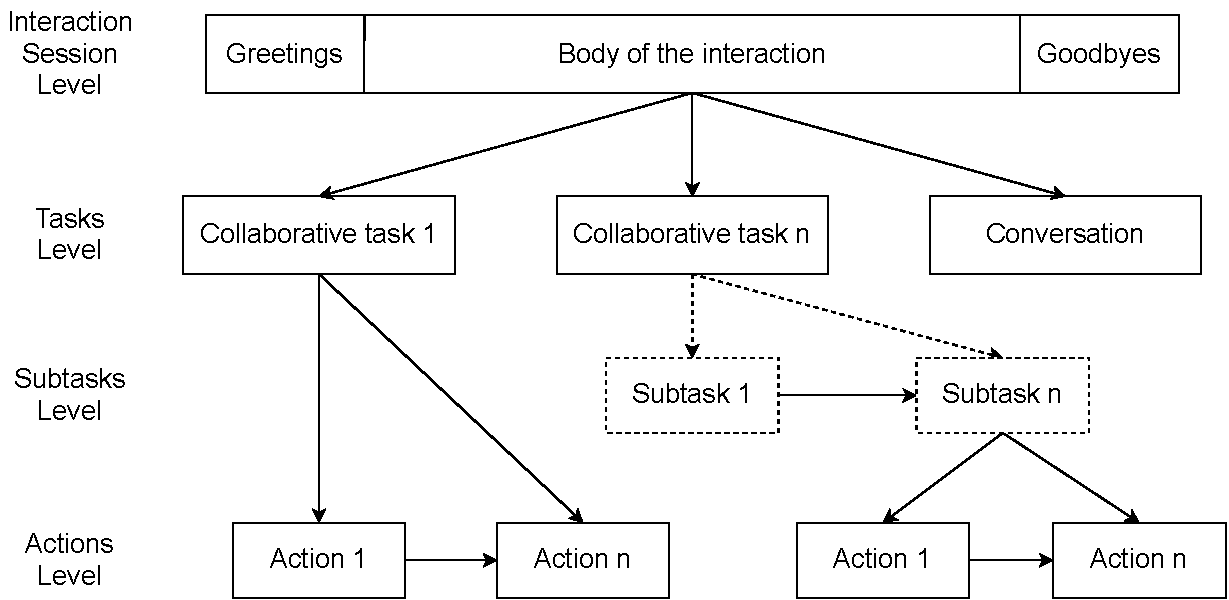
\includegraphics[width=\linewidth]{figures/chapter2/session_interaction.pdf}
	\caption{The hierarchical structure of an interaction session. The highest level is the interaction session. The second level is composed of the tasks. They are included in the body of interaction of the interaction session and, two types of tasks are considered and may overlap, collaborative and conversational tasks. With this representation, a task can be recursively refined as subtasks until reaching the last level, the actions level, which is considered as atomic.
%		Subtasks are not considered as a ``real'' level of the interaction session, specially to evaluate the \acrshort{qoi}, as it may exist or not according to the task.
		}
	\label{fig:levels}
\end{figure}


\subsection{Representation of a Human-Robot Interaction Session}
We define an \textbf{interaction session} as the period during which the robot and a human interact together and are engaged. It is divided in three parts, following the structure proposed by Robinson~\cite{robinson_overall_2012} as presented in Section~\ref{chap2:sec:soc_inter}: the greetings, the body of the interaction and the goodbyes. First, \textit{the greetings} corresponds to the period where an agent starts an interaction by initiating it with another agent. The interaction session lasts as long as the interactants are maintaining the interaction through conversation and collaborative tasks performance which corresponds to the \textit{body of interaction}. Finally it ends when at least one of the interactants is disengaged, either by abruptly ending the interaction or by closing the interaction as described by Schegloff and Sacks~\cite{schegloff_1973_opening}, it corresponds to ``the goodbyes''. For example, for an entertainment robot in a mall, an \textit{interaction session} starts when a person signals to the robot that they want to engage, by greeting it or by approaching it and looking at it. The body of interaction is composed of conversation and eventually direction-giving tasks and, the session lasts until the person says goodbye or leaves. This is the nominal case and, the duty of the robot is to contribute to maintain the session alive until the human decides to close it, because it is at the service of humans. However, in some (extreme) cases, the robot might decide to close the interaction by itself.

Moreover, as seen in Section~\ref{chap1:subsubsec:joint_commit}, social interactions and joint activities (or actions) involve commitment, or rather engagement as we say in robotics -- this difference in the vocabulary as been highlighted in~\cite{castro_2019_commitments}. As explained in the previous chapter, there is no unique definition of what it means to be engaged. We chose one that is frequently used in robotics, proposed by Sidner and Lee~\cite{sidner_2003_engagement}: ``Engagement is the process by which two (or more) participants establish, maintain and end their perceived connection during interactions they jointly undertake''. The robot must be able to exhibit its engagement and disengagement and also to assess them with respect to its human partner.

To consider engagement, we defined three states for the body of interaction, corresponding to what can happen during the latter: 
\begin{bulletList}
	\item conversation: a social chit-chat or a goal negotiation, without any physical action performed except communicative gestures
	\item collaborative task: both agents executing actions in order to achieve a shared goal
	\item idle phases: the agents are not chatting or performing a collaborative task together but remain engaged in the interaction session, it happens in-between active interaction phases
\end{bulletList}

For each of these three states, the way to exhibit the engagement varies (\eg in a conversation, an agent looking at their partner displays their engagement; during a task, an agent correctly performing their action is a way to demonstrate their engagement). That is why there is a need to define what behavior the robot has to exhibit in each state and what behavior it should expect from the human in each state, as these behaviors are usually very specific (\eg in a direction-giving task, the robot keeps its head oriented toward its partner's face to demonstrate its engagement in conversation and idle contexts and when it gives a direction it expects the human to look at the direction it is showing; in a stack task, when the robot gives an instruction it expects the human to take a given cube).

Transitions from one state to another can be managed by triggers more or less complex. For example, a collaborative task can be initiated when a human asks the robot that they achieve a goal together.


\subsection{Collaborative Tasks, Substasks and Actions}
\textbf{\textit{Tasks}} compose the body of the interaction of an interaction session as shown in Fig.~\ref{fig:levels}. As mentioned in the previous paragraph, we distinguish conversation (\ie agents engage in dialogue to exchange ideas, or to ask questions) from collaborative tasks (\ie agents work as partners, collaborating to perform tasks and to achieve common goals). We will not develop more on conversation since it is not the main focus of this work.

In joint or collaborative activities (see Section~\ref{chap1:subsec:def_ja}), humans are committed to achieve a goal together, involving collaboration and shared plans as shown in Section~\ref{chap1:sec:ja}. In the human-robot interaction case, the same mechanisms are in play in humans, as they are essential to successful collaboration. When a human and a robot perform a task together, as described by Bauer \textit{et al}.~\cite{bauer_2008_collab}, we could say that the robot has the intent to help the human, so the human's intention becomes its own intention. Then, they have the joint intention to reach a common goal and, as shown by Michael and Salice~\cite{michael_2017_commitment}, they have a commitment to the joint activity, leading to perform joint actions. Therefore, during its evaluation and decision-making processes, the robot has to take into account that the human and itself should remain engaged all along an interaction session for the tasks to be successful and both have to manage and contribute to maintain expectations about what the other is doing. 

The elements composing a \textit{task} are: a goal, a plan and involved agents. A plan is needed to achieve a goal. The ones we manipulate are \acrshort{htn}-based plans, composed of \emph{abstract tasks} that we also call \emph{subtasks} and \emph{primitive tasks} that we also call \emph{actions}.

\textbf{\textit{Actions}} are the elementary items of tasks, \emph{primitive tasks}, manipulated by the high-level robot supervision controller. They cannot be decomposed further by it (\eg placement and motion planning are achieved by a lower control system not described here). It is usual to describe an action with its preconditions, its effects and, the agents and entities implied in its execution (\eg in plans written in PDDL (Planning Domain Definition Language)~\cite{ghallab_98_pddl}). We add to this description the notion of expected reactions (which can themselves be actions) from the other agents once the action is executed.

In our model, an agent (human or robot) is a contributor to the task and has a mental state as described by Devin \textit{et al}.~\cite{devin_2016_implemented}. The mental state is a set of facts representing, from the agent point of view, the current world state, the state of the goal and the current task state. Since we are interested here in the robot situation assessment and decisional processes, the mental state of the human is built and managed by the robot as an estimation of the beliefs of the human~\cite{milliez_2014_framework, hiatt_2017_modeling,tabrez_2020}.

\section{The Structure of JAHRVIS}\label{chap5:sec:jahrvis}
%\section{The Architecture of JAHRVIS}\label{chap5:sec:jahrvis}
The \acrfull{jahrvis} is implemented on top of our ROS-Jason framework\footnote{\url{https://github.com/amdia/ld_rjs}}. During the design of \acrshort{jahrvis}, we identified seven high-level features we needed and implemented their associated processes, based on the objectives presented in Section~\ref{chap5:sec:sup_features}\footnote{The design of \acrshort{jahrvis} was an iterative work, indeed the first version being the supervisor implemented for the task described in Chapter~\ref{chapter:chap8}, the second one was the supervisor of the task described in Chapter~\ref{chapter:chap9} and the final one was the supervisor of the example used all along Chapter~\ref{chapter:chap6}}. We present \acrshort{jahrvis} structure in Figure~\ref{chap5:fig:sup_overview}, with the seven processes in blue; the \acrshort{qoi} Evaluator is dedicated to the interaction evaluation and the six others are dedicated to the decision and control. All the next developments of this chapter will be about the description of these processes. The components not in blue are external components from the robotic architecture presented in Section~\ref{chap3:sec:rob_archi}. They bring to \acrshort{jahrvis} additional features of knowledge maintenance, decision-making and execution.

\begin{figure}[!ht]
	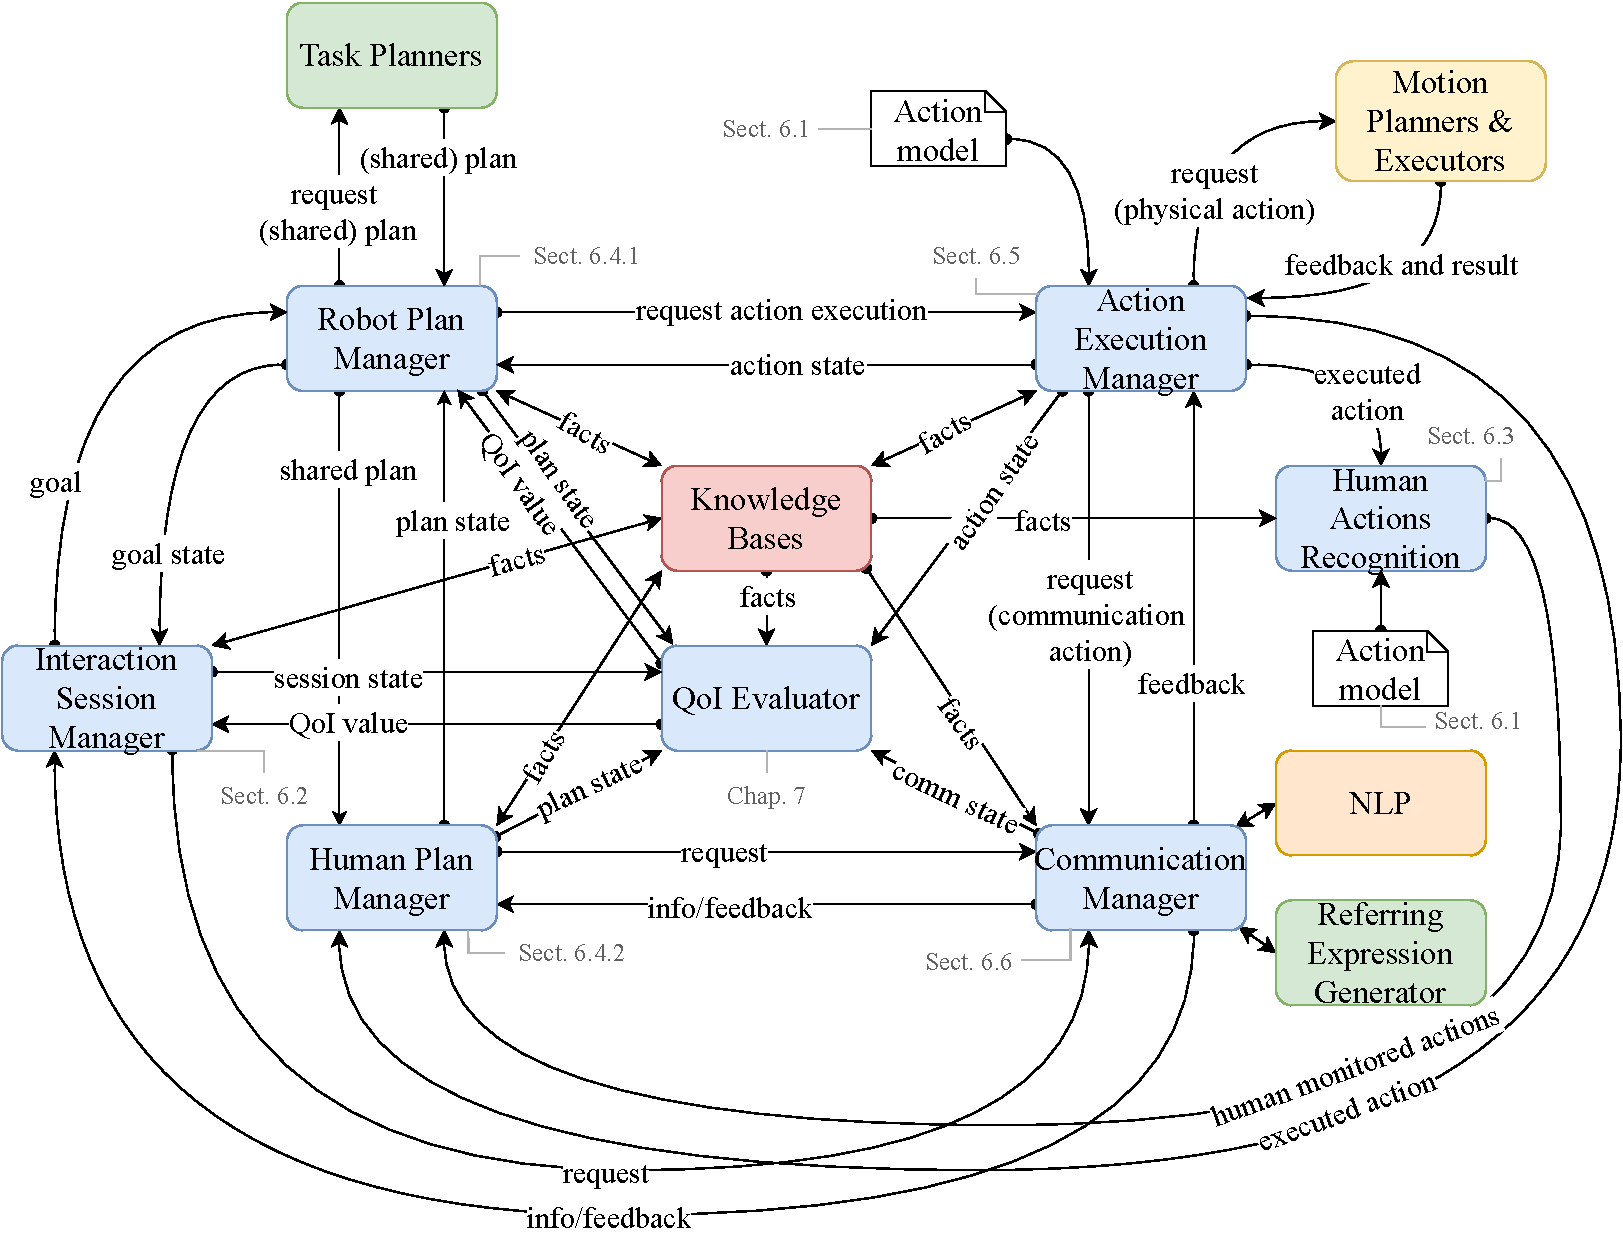
\includegraphics[width=\linewidth]{figures/chapter2/supervisor_modules.pdf}
	\caption{The \acrshort{jahrvis} processes (in blue) and their interactions between themselves and with the other components of the robotic architecture presented in Section~\ref{chap3:sec:rob_archi}.}
	\label{chap5:fig:sup_overview}
\end{figure}

For each process (in blue in Figure~\ref{chap5:fig:sup_overview}), we implemented a \acrfull{rja}, with the desired behavior coded in ASL and the needed customizations added in Java. Thus, internal communications between the \acrshort{jahrvis} processes, and so \acrshort{rja}s, use Jason messages (see Section~\ref{chap4:subsec:jason}). External communication with the other components of the robotic architecture is based on either ROS messages, services or action clients.

Not all \acrshort{rja}s are active at each level of interaction defined in Section~\ref{chap5:sec:levels}. Indeed, as its name suggests, the \textit{Interaction Session Manager} handles interaction sessions. The \textit{Robot} and \textit{Human Plan Managers} handle the task level. And, the \textit{Action Execution Manager} and the \textit{\acrlong{ham}} are in charge of the action level. The \textit{Communication Manager} is active at all levels. We can also make the distinction between the component dedicated to the assessment of the quality of interaction, \ie the \acrshort{qoi} Evaluator which will be described in Chapter~\ref{chapter:chap7}, and all the other ones, dedicated to the decision-making and control.

Figure~\ref{chap5:fig:data_state} shows an overview of the data representing the state of \acrshort{jahrvis} at each instant when the system runs. The robot can either be in an interaction session with a human or be by itself. When it is in an interaction session, it computes the human's commitment (it may be a simple function checking if the human is here or not) and is available to perform collaborative tasks. When the robot is not interacting with humans, it can have tasks to perform such as going to its home base. If a collaborative task should start (on human request or on the robot's initiative), a (shared) plan is obtained from the Task Planner as shown in Figure~\ref{chap5:fig:sup_overview}. When the collaborative task is ongoing, the robot has its beliefs about the environment and the plan progress, and estimates the human's ones. Beliefs about the environment are provided by other components of the robotic architecture presented in Section~\ref{chap3:sec:rob_archi}: the Situation Assessment and the Knowledge Bases. Each abstract and primitive task has a number of data associated to it. Moreover, \acrlong{qoi} and human action recognition are continuously processed. Finally, when an action is executed by the Motion Planners and Executors, updates about the action states are communicated to \acrshort{jahrvis}.

\begin{figure}[!ht]
	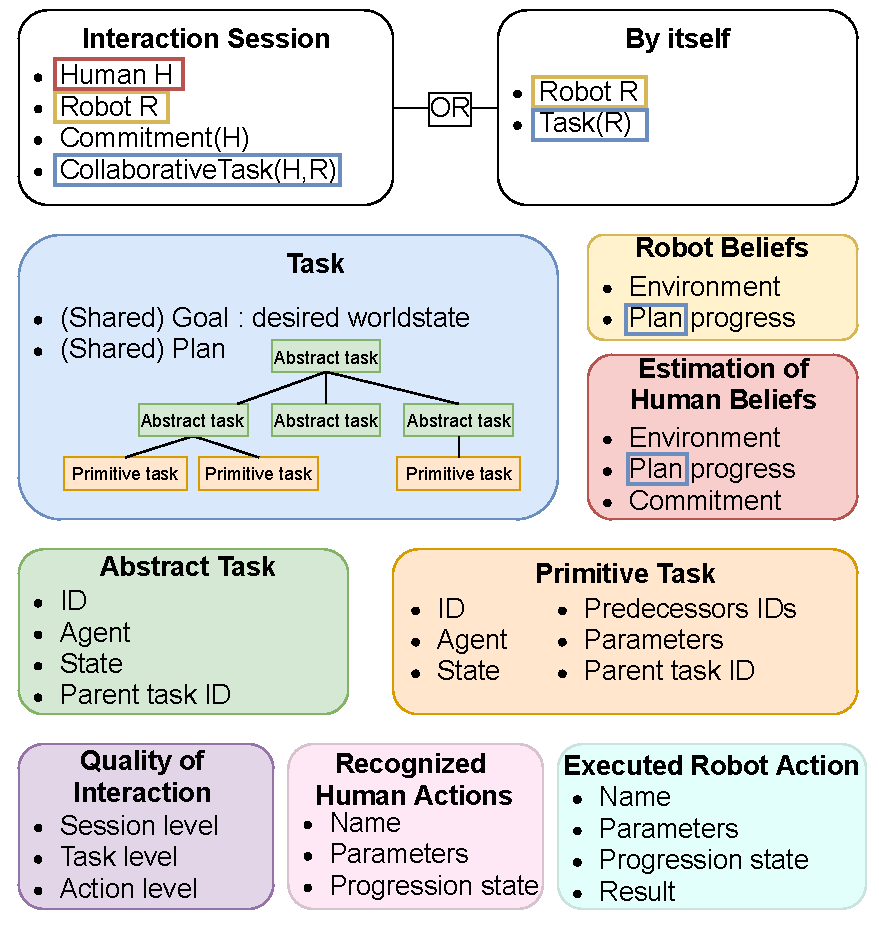
\includegraphics[width=\linewidth]{figures/chapter2/data_state_representation.pdf}
	\caption{Overview of the data representing the state of \acrshort{jahrvis} at each instant when the system runs. The robot can either be in an interaction session with a human or be by itself. When it is in a task, plan progress are maintained from the robot's and human's estimated point of views. A plan is composed of abstract and primitive tasks whose state evolved during the task. \acrshort{qoi} and human action recognition are two elements continuously computed. When the robot executes an action, the state of the later is updated as well as its result (success or failure).}
	\label{chap5:fig:data_state}
\end{figure}

In the Chapters~\ref{chapter:chap6} and \ref{chapter:chap7} will be presented these processes. Chapter~\ref{chapter:chap6} introduces the ones related to the decision-making and robot control while Chapter~\ref{chapter:chap7} describe the evaluation process of the \acrlong{qoi}. Chapter~\ref{chapter:chap6} will start by laying the foundations for the \acrshort{rja} functioning: the knowledge representations and management. Then, each \acrshort{rja} will be thoroughly described. The \acrfull{ism} is dedicated to in-between tasks, \ie the opening and closing of interactions and all the dialog which can happen between two collaborative tasks. When a shared goal is established, the shared plan is handled by the \acrfull{rpm} and the \acrfull{hpm}, \ie to follow the plan progression, to make sure that the observed human actions match the ones of the plan and to decide when the robot should act. Robot actions to perform are sent to the \acrfull{aem} that interfaces with the motion planers and executors. As for human actions, they are monitored and recognized by the \acrfull{ham}. Finally, the \acrfull{cm} is in charge of producing the communication for the human when requested by another \acrshort{rja} along with the human communication reception.




\ifdefined\included
\else
\bibliographystyle{acm}
\bibliography{These}
\end{document}
\fi







\ifdefined\included
\else
\documentclass[a4paper,11pt,twoside]{StyleThese}
\usepackage{amsmath,amssymb, amsthm}             % AMS Math
\usepackage[T1]{fontenc}
\usepackage[utf8x]{inputenc}
\usepackage{babel}
\usepackage{datetime}

\usepackage{silence}

\WarningFilter{minitoc(hints)}{W0023}
\WarningFilter{minitoc(hints)}{W0028}
\WarningFilter{minitoc(hints)}{W0030}

\usepackage{lmodern}
\usepackage{tabularx}
%\usepackage{tabular}
\usepackage{multirow}
\usepackage{xspace}

\usepackage{subfig}
\usepackage[inline]{enumitem}

\usepackage{hhline}
\usepackage[left=1.5in,right=1.3in,top=1.1in,bottom=1.1in,includefoot,includehead,headheight=13.6pt]{geometry}
\renewcommand{\baselinestretch}{1.05}

% Table of contents for each chapter

\usepackage[nottoc, notlof, notlot]{tocbibind}
\usepackage{minitoc}
\setcounter{minitocdepth}{2}
\mtcindent=15pt
% Use \minitoc where to put a table of contents

\usepackage{aecompl}

% Glossary / list of abbreviations

\usepackage[intoc]{nomencl}
\iftoggle{ThesisInEnglish}{%
\renewcommand{\nomname}{Glossary}
}{ %
\renewcommand{\nomname}{Liste des Abréviations}
}

\usepackage{etoolbox}
\renewcommand\nomgroup[1]{%
  \item[\bfseries
  \ifstrequal{#1}{A}{Number Sets}{%
  \ifstrequal{#1}{G}{Agents Beliefs and Action Models}{%
  \ifstrequal{#1}{N}{Navigation}{%
  \ifstrequal{#1}{O}{Ontology}{%
  \ifstrequal{#1}{R}{Referring Expression Generation}{%
  \ifstrequal{#1}{Z}{Controllable and Uncontrollable Agents Task Planning}{}}}}}}%
]}

\makenomenclature



% My pdf code

\usepackage{ifpdf}

\ifpdf
  \usepackage[pdftex]{graphicx}
  \DeclareGraphicsExtensions{.jpg}
  \usepackage[pagebackref,hyperindex=true]{hyperref}
  \usepackage{tikz}
  \usetikzlibrary{arrows,shapes,calc}
\else
  \usepackage{graphicx}
  \DeclareGraphicsExtensions{.ps,.eps}
  \usepackage[dvipdfm,pagebackref,hyperindex=true]{hyperref}
\fi

\graphicspath{{.}{images/}}

%% nicer backref links. NOTE: The flag ThesisInEnglish is used to define the
% language in the back references. Read more about it in These.tex

\iftoggle{ThesisInEnglish}{%
\renewcommand*{\backref}[1]{}
\renewcommand*{\backrefalt}[4]{%
\ifcase #1 %
(Not cited.)%
\or
(Cited in page~#2.)%
\else
(Cited in pages~#2.)%
\fi}
\renewcommand*{\backrefsep}{, }
\renewcommand*{\backreftwosep}{ and~}
\renewcommand*{\backreflastsep}{ and~}
}{%
\renewcommand*{\backref}[1]{}
\renewcommand*{\backrefalt}[4]{%
\ifcase #1 %
(Non cité.)%
\or
(Cité en page~#2.)%
\else
(Cité en pages~#2.)%
\fi}
\renewcommand*{\backrefsep}{, }
\renewcommand*{\backreftwosep}{ et~}
\renewcommand*{\backreflastsep}{ et~}
}

% Links in pdf
\usepackage{color}
\definecolor{linkcol}{rgb}{0,0,0.4} 
\definecolor{citecol}{rgb}{0.5,0,0} 
\definecolor{linkcol}{rgb}{0,0,0} 
\definecolor{citecol}{rgb}{0,0,0}
% Change this to change the informations included in the pdf file

\hypersetup
{
bookmarksopen=true,
pdftitle="Endowing the robot with the abilities to control and evaluate its contribution to a human-robot joint action",
pdfauthor="Amandine MAYIMA", %auteur du document
pdfsubject="Thèse", %sujet du document
%pdftoolbar=false, %barre d'outils non visible
pdfmenubar=true, %barre de menu visible
pdfhighlight=/O, %effet d'un clic sur un lien hypertexte
colorlinks=true, %couleurs sur les liens hypertextes
pdfpagemode=None, %aucun mode de page
pdfpagelayout=SinglePage, %ouverture en simple page
pdffitwindow=true, %pages ouvertes entierement dans toute la fenetre
linkcolor=linkcol, %couleur des liens hypertextes internes
citecolor=citecol, %couleur des liens pour les citations
urlcolor=linkcol %couleur des liens pour les url
}

% definitions.
% -------------------

\setcounter{secnumdepth}{3}
\setcounter{tocdepth}{2}

% Some useful commands and shortcut for maths:  partial derivative and stuff

\newcommand{\pd}[2]{\frac{\partial #1}{\partial #2}}
\def\abs{\operatorname{abs}}
\def\argmax{\operatornamewithlimits{arg\,max}}
\def\argmin{\operatornamewithlimits{arg\,min}}
\def\diag{\operatorname{Diag}}
\newcommand{\eqRef}[1]{(\ref{#1})}

\usepackage{rotating}                    % Sideways of figures & tables
%\usepackage{bibunits}
%\usepackage[sectionbib]{chapterbib}          % Cross-reference package (Natural BiB)
%\usepackage{natbib}                  % Put References at the end of each chapter
                                         % Do not put 'sectionbib' option here.
                                         % Sectionbib option in 'natbib' will do.
\usepackage{fancyhdr}                    % Fancy Header and Footer

% \usepackage{txfonts}                     % Public Times New Roman text & math font
  
%%% Fancy Header %%%%%%%%%%%%%%%%%%%%%%%%%%%%%%%%%%%%%%%%%%%%%%%%%%%%%%%%%%%%%%%%%%
% Fancy Header Style Options

\pagestyle{fancy}                       % Sets fancy header and footer
\fancyfoot{}                            % Delete current footer settings

%\renewcommand{\chaptermark}[1]{         % Lower Case Chapter marker style
%  \markboth{\chaptername\ \thechapter.\ #1}}{}} %

%\renewcommand{\sectionmark}[1]{         % Lower case Section marker style
%  \markright{\thesection.\ #1}}         %

\fancyhead[LE,RO]{\bfseries\thepage}    % Page number (boldface) in left on even
% pages and right on odd pages
\fancyhead[RE]{\bfseries\nouppercase{\leftmark}}      % Chapter in the right on even pages
\fancyhead[LO]{\bfseries\nouppercase{\rightmark}}     % Section in the left on odd pages

\let\headruleORIG\headrule
\renewcommand{\headrule}{\color{black} \headruleORIG}
\renewcommand{\headrulewidth}{1.0pt}
\usepackage{colortbl}
\arrayrulecolor{black}

\fancypagestyle{plain}{
  \fancyhead{}
  \fancyfoot{}
  \renewcommand{\headrulewidth}{0pt}
}

%\usepackage{MyAlgorithm}
%\usepackage[noend]{MyAlgorithmic}
\usepackage{algorithm}
\usepackage[noend]{algpseudocode}
\usepackage{comment}
\usepackage[ED=MITT-InfoTel, Ets=INSA]{tlsflyleaf}
%%% Clear Header %%%%%%%%%%%%%%%%%%%%%%%%%%%%%%%%%%%%%%%%%%%%%%%%%%%%%%%%%%%%%%%%%%
% Clear Header Style on the Last Empty Odd pages
\makeatletter

\def\cleardoublepage{\clearpage\if@twoside \ifodd\c@page\else%
  \hbox{}%
  \thispagestyle{empty}%              % Empty header styles
  \newpage%
  \if@twocolumn\hbox{}\newpage\fi\fi\fi}

\newcommand*{\algrule}[1][\algorithmicindent]{%
	\makebox[#1][l]{%
		\hspace*{.2em}% <------------- This is where the rule starts from
		\vrule height .75\baselineskip depth .25\baselineskip
	}
}

%%% to have lines in algorithm, from stackexchange
\newcount\ALG@printindent@tempcnta
\def\ALG@printindent{%
	\ifnum \theALG@nested>0% is there anything to print
	\ifx\ALG@text\ALG@x@notext% is this an end group without any text?
	% do nothing
	\else
	\unskip
	% draw a rule for each indent level
	\ALG@printindent@tempcnta=1
	\loop
	\algrule[\csname ALG@ind@\the\ALG@printindent@tempcnta\endcsname]%
	\advance \ALG@printindent@tempcnta 1
	\ifnum \ALG@printindent@tempcnta<\numexpr\theALG@nested+1\relax
	\repeat
	\fi
	\fi
}
% the following line injects our new indent handling code in place of the default spacing
\patchcmd{\ALG@doentity}{\noindent\hskip\ALG@tlm}{\ALG@printindent}{}{\errmessage{failed to patch}}
\patchcmd{\ALG@doentity}{\item[]\nointerlineskip}{}{}{} % no spurious vertical space
% end vertical rule patch for algorithmicx

\makeatother
 
%%%%%%%%%%%%%%%%%%%%%%%%%%%%%%%%%%%%%%%%%%%%%%%%%%%%%%%%%%%%%%%%%%%%%%%%%%%%%%% 
% Prints your review date and 'Draft Version' (From Josullvn, CS, CMU)
\newcommand{\reviewtimetoday}[2]{\special{!userdict begin
    /bop-hook{gsave 20 710 translate 45 rotate 0.8 setgray
      /Times-Roman findfont 12 scalefont setfont 0 0   moveto (#1) show
      0 -12 moveto (#2) show grestore}def end}}
% You can turn on or off this option.
% \reviewtimetoday{\today}{Draft Version}
%%%%%%%%%%%%%%%%%%%%%%%%%%%%%%%%%%%%%%%%%%%%%%%%%%%%%%%%%%%%%%%%%%%%%%%%%%%%%%% 

\newenvironment{maxime}[1]
{
\vspace*{0cm}
\hfill
\begin{minipage}{0.5\textwidth}%
%\rule[0.5ex]{\textwidth}{0.1mm}\\%
\hrulefill $\:$ {\bf #1}\\
%\vspace*{-0.25cm}
\it 
}%
{%

\hrulefill
\vspace*{0.5cm}%
\end{minipage}
}

\let\minitocORIG\minitoc
\renewcommand{\minitoc}{\minitocORIG \vspace{1.5em}}

\usepackage{multirow}
%\usepackage{slashbox}

\newenvironment{bulletList}%
{ \begin{list}%
	{\tiny$\bullet$}%
	{\setlength{\labelwidth}{25pt}%
	 \setlength{\leftmargin}{30pt}%
	 \setlength{\itemsep}{-0.5em}}}%
{ \end{list} }

\newenvironment{inlineEnumerate}
{\begin{enumerate*} [label={(\arabic*)}] }
{\end{enumerate*}}

\theoremstyle{definition}
\newtheorem{definition}{Definition}
\renewcommand{\epsilon}{\varepsilon}

% centered page environment

\newenvironment{vcenterpage}
{\newpage\vspace*{\fill}\thispagestyle{empty}\renewcommand{\headrulewidth}{0pt}}
{\vspace*{\fill}}

\newenvironment{asl}{\ttfamily\begin{tabbing}~~~\=$\leftarrow$ \= ~~~ \=
		\kill}{\end{tabbing}}

\usepackage{tablefootnote}

\theoremstyle{plain}
\newtheorem{constraint}{Constraint}[section]

\algnewcommand\algorithmicforeach{\textbf{for each}}
\algnewcommand\algorithmicin{\textbf{in}}
\algdef{S}[FOR]{ForEach}[2]{\algorithmicforeach\ #1\ \algorithmicin\ #2\ \algorithmicdo}

\algnewcommand\algorithmicforkxor{\textbf{do fork-join-xor}}
\algnewcommand\algorithmicendforkxor{\textbf{end fork-join-xor}}
\algdef{SE}{ForkXor}{EndForkXor}{\algorithmicforkxor}{\algorithmicendforkxor}


\usepackage{listings}
\lstset{
	frame=single,
	captionpos=b,
	breaklines=true,
	basicstyle=\ttfamily,
	numberstyle=\color{black},
	tabsize=2,
	mathescape=true,
	literate=%
		{â}{{\^a}}1
}

\lstdefinestyle{inline}{
	frame=none,
	aboveskip=\smallskipamount,
	belowskip=\smallskipamount,
}

\lstdefinestyle{OwlTurtle}{
	language=C,
	tabsize=4,
	basicstyle=\scriptsize\ttfamily,
	keywordstyle=\bfseries\color{darkgray},
	morekeywords={rdf:type, rdfs:domain, rdfs:subPropertyOf, rdfs:range, :hasSubtask, :DecompositionUsedBy, rdfs:subClassOf, :hasDecomposition, owl:inverseOf, htn_actions:hasEffect, rdfs:label},
	alsoletter=:
}

\lstdefinestyle{aslDef}{
	frame=none,
%	breaklines=false,
	%xleftmargin=.1\textwidth, xrightmargin=.1\textwidth
}

\fancypagestyle{example}{%
	\fancyhead[LE]{\bfseries\thepage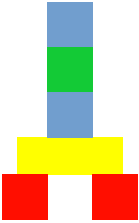
\includegraphics[scale=0.20]{figures/chapter2/task_goal.pdf}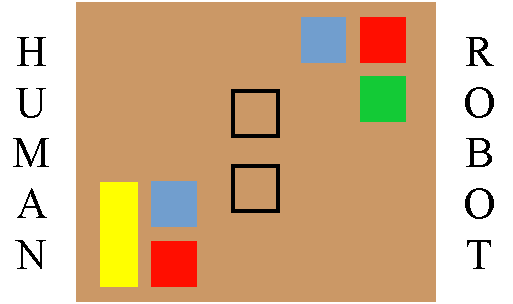
\includegraphics[scale=0.18]{figures/chapter2/task_setup_mini.pdf}}   
	\fancyhead[RO]{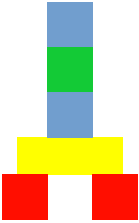
\includegraphics[scale=0.20]{figures/chapter2/task_goal.pdf}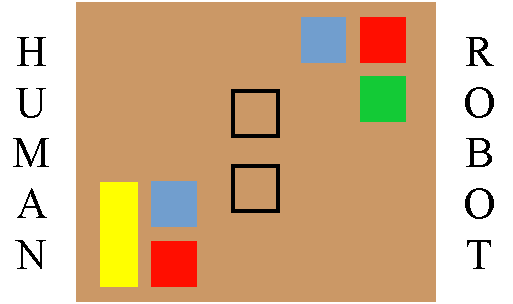
\includegraphics[scale=0.18]{figures/chapter2/task_setup_mini.pdf}\bfseries\thepage}  
	\fancyhead[RE]{\bfseries\nouppercase{\leftmark}}      % Chapter in the right on even pages
	\fancyhead[LO]{\bfseries\nouppercase{\rightmark}}     % Section in the left on odd pages
}%

\usepackage{pdfpages}
\usepackage{makecell}
\usepackage{pdflscape} 
\usepackage{mathtools}
\usepackage[section]{placeins}
\usepackage{afterpage}

%%%%%%%% my commands
\newcommand{\etal}{\textit{et al}.}
\newcommand{\ie}{\textit{i.e.}, }
\newcommand{\eg}{\textit{e.g.}, }
\newcommand{\fact}[3]{\mbox{\textit{#1}(#2, #3)}}
\newcommand{\circledtext}[1]{\raisebox{.5pt}{\textcircled{\raisebox{-.9pt} {#1}}}}
\newcommand{\sparql}{\textsc{SPARQL}}

\newcommand{\algConst}[1]{${\scriptscriptstyle #1}$}
\newcommand{\algNormTextSub}[2]{$\text{#1}_{#2}$}

\newcommand{\aslnumber}[1]{$#1$}
\newcommand{\aslstring}[1]{\textsf{#1}}
\newcommand{\aslvar}[1]{\textcolor{purple}{\textit{#1}}}
\newcommand{\asllabel}[1]{\textbf{#1}}
\newcommand{\annotation}[1]{{\footnotesize #1}}
\newcommand{\rulebody}[1]{\mbox{\hspace{.05\linewidth}}\begin{minipage}[t]{0.9\linewidth}#1.\end{minipage}}
\newcommand{\context}[1]{\begin{minipage}[t]{0.9\linewidth}#1\end{minipage}}
\newcommand{\planbody}[1]{\begin{minipage}[t]{0.9\linewidth}#1.\end{minipage}}
\newcommand{\Jason}[0]{\textbf{\textit{Jason}}}
\newcommand{\sn}{\mbox{\large\textbf{\texttt{\textasciitilde}}}}


\sloppy
\begin{document}
	\setcounter{chapter}{5} %% Numéro du chapitre précédent ;)
	\dominitoc
	\faketableofcontents
	\fi

\chapter{How JAHRVIS work}\label{chapter:chap6}
\minitoc

The objective of this chapter is to present the \acrshort{jahrvis} processes involved in the decision-making and the control of the robot when jointly interacting with a human. First, we present the knowledge representations used, then the \acrlong{ism}, the \acrlong{ham}, the Shared Plans Handling composed of two processes, one for the robot (\acrlong{rpm}) and one for the human (\acrlong{hpm}), the \acrlong{aem}, and finally the \acrlong{cm}.

Most examples given in this chapter will base themselves on a collaborative task, the \textit{BuildingTask}, that we are going to present now. It has been inspired by~\cite{devin_2017_decisions}. A human and a robot have to build a block construction together as represented in Figure~\ref{chap6:subfig:task_goal}. At the beginning of the task, the robot and the human have several colored cubes (the yellow one will be referred to as a stick) they can access as in a set-up like the one illustrated in Figure~\ref{chap6:subfig:task_setup}. Two identical placements are set on the table to indicate where to put the two red cubes which are the first ones to place. Each agent has 3 available actions: Pick, Place and Wait. They can only access to the cube on their side of the table. Figure~\ref{chap6:fig:building_task} is a picture of the task being performed with a human and a PR2 robot. The PR2 robot executes the task fully autonomously, thanks to the robotic architecture presented in Section~\ref{chap3:sec:rob_archi}. A video of the task with the robot running completely autonomously can be seen\footnote{Link to come}.

\begin{figure}[!htb]
%	\centering
	\hspace*{\fill}%
	\subfloat[Goal of the task (side view)]{\label{chap6:subfig:task_goal}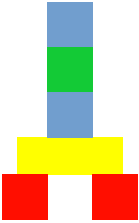
\includegraphics[width=0.2\linewidth]{figures/chapter2/task_goal.pdf}}\hfill
	\subfloat[Initial set-up (top view)]{\label{chap6:subfig:task_setup}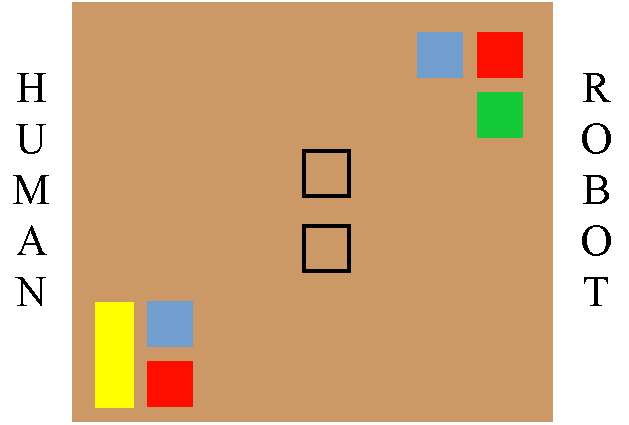
\includegraphics[width=0.5\linewidth]{figures/chapter2/task_setup.pdf}}
	\hspace*{\fill}
	\caption{Description of the blocks building task. The human and the robot have to build the stack together. We assume that the robot and the human know where all the available blocks are. We would like the robot to adapt as much as possible to the human actions and decisions while avoiding useless or tiresome verbal interactions.}
	\label{chap6:fig:task_blocks}
\end{figure}

Figure~\ref{chap6:fig:task_blocks} will be reminded in page headers where the BuildingTask example will be mentioned.

\begin{figure}[!ht]
	\centering
	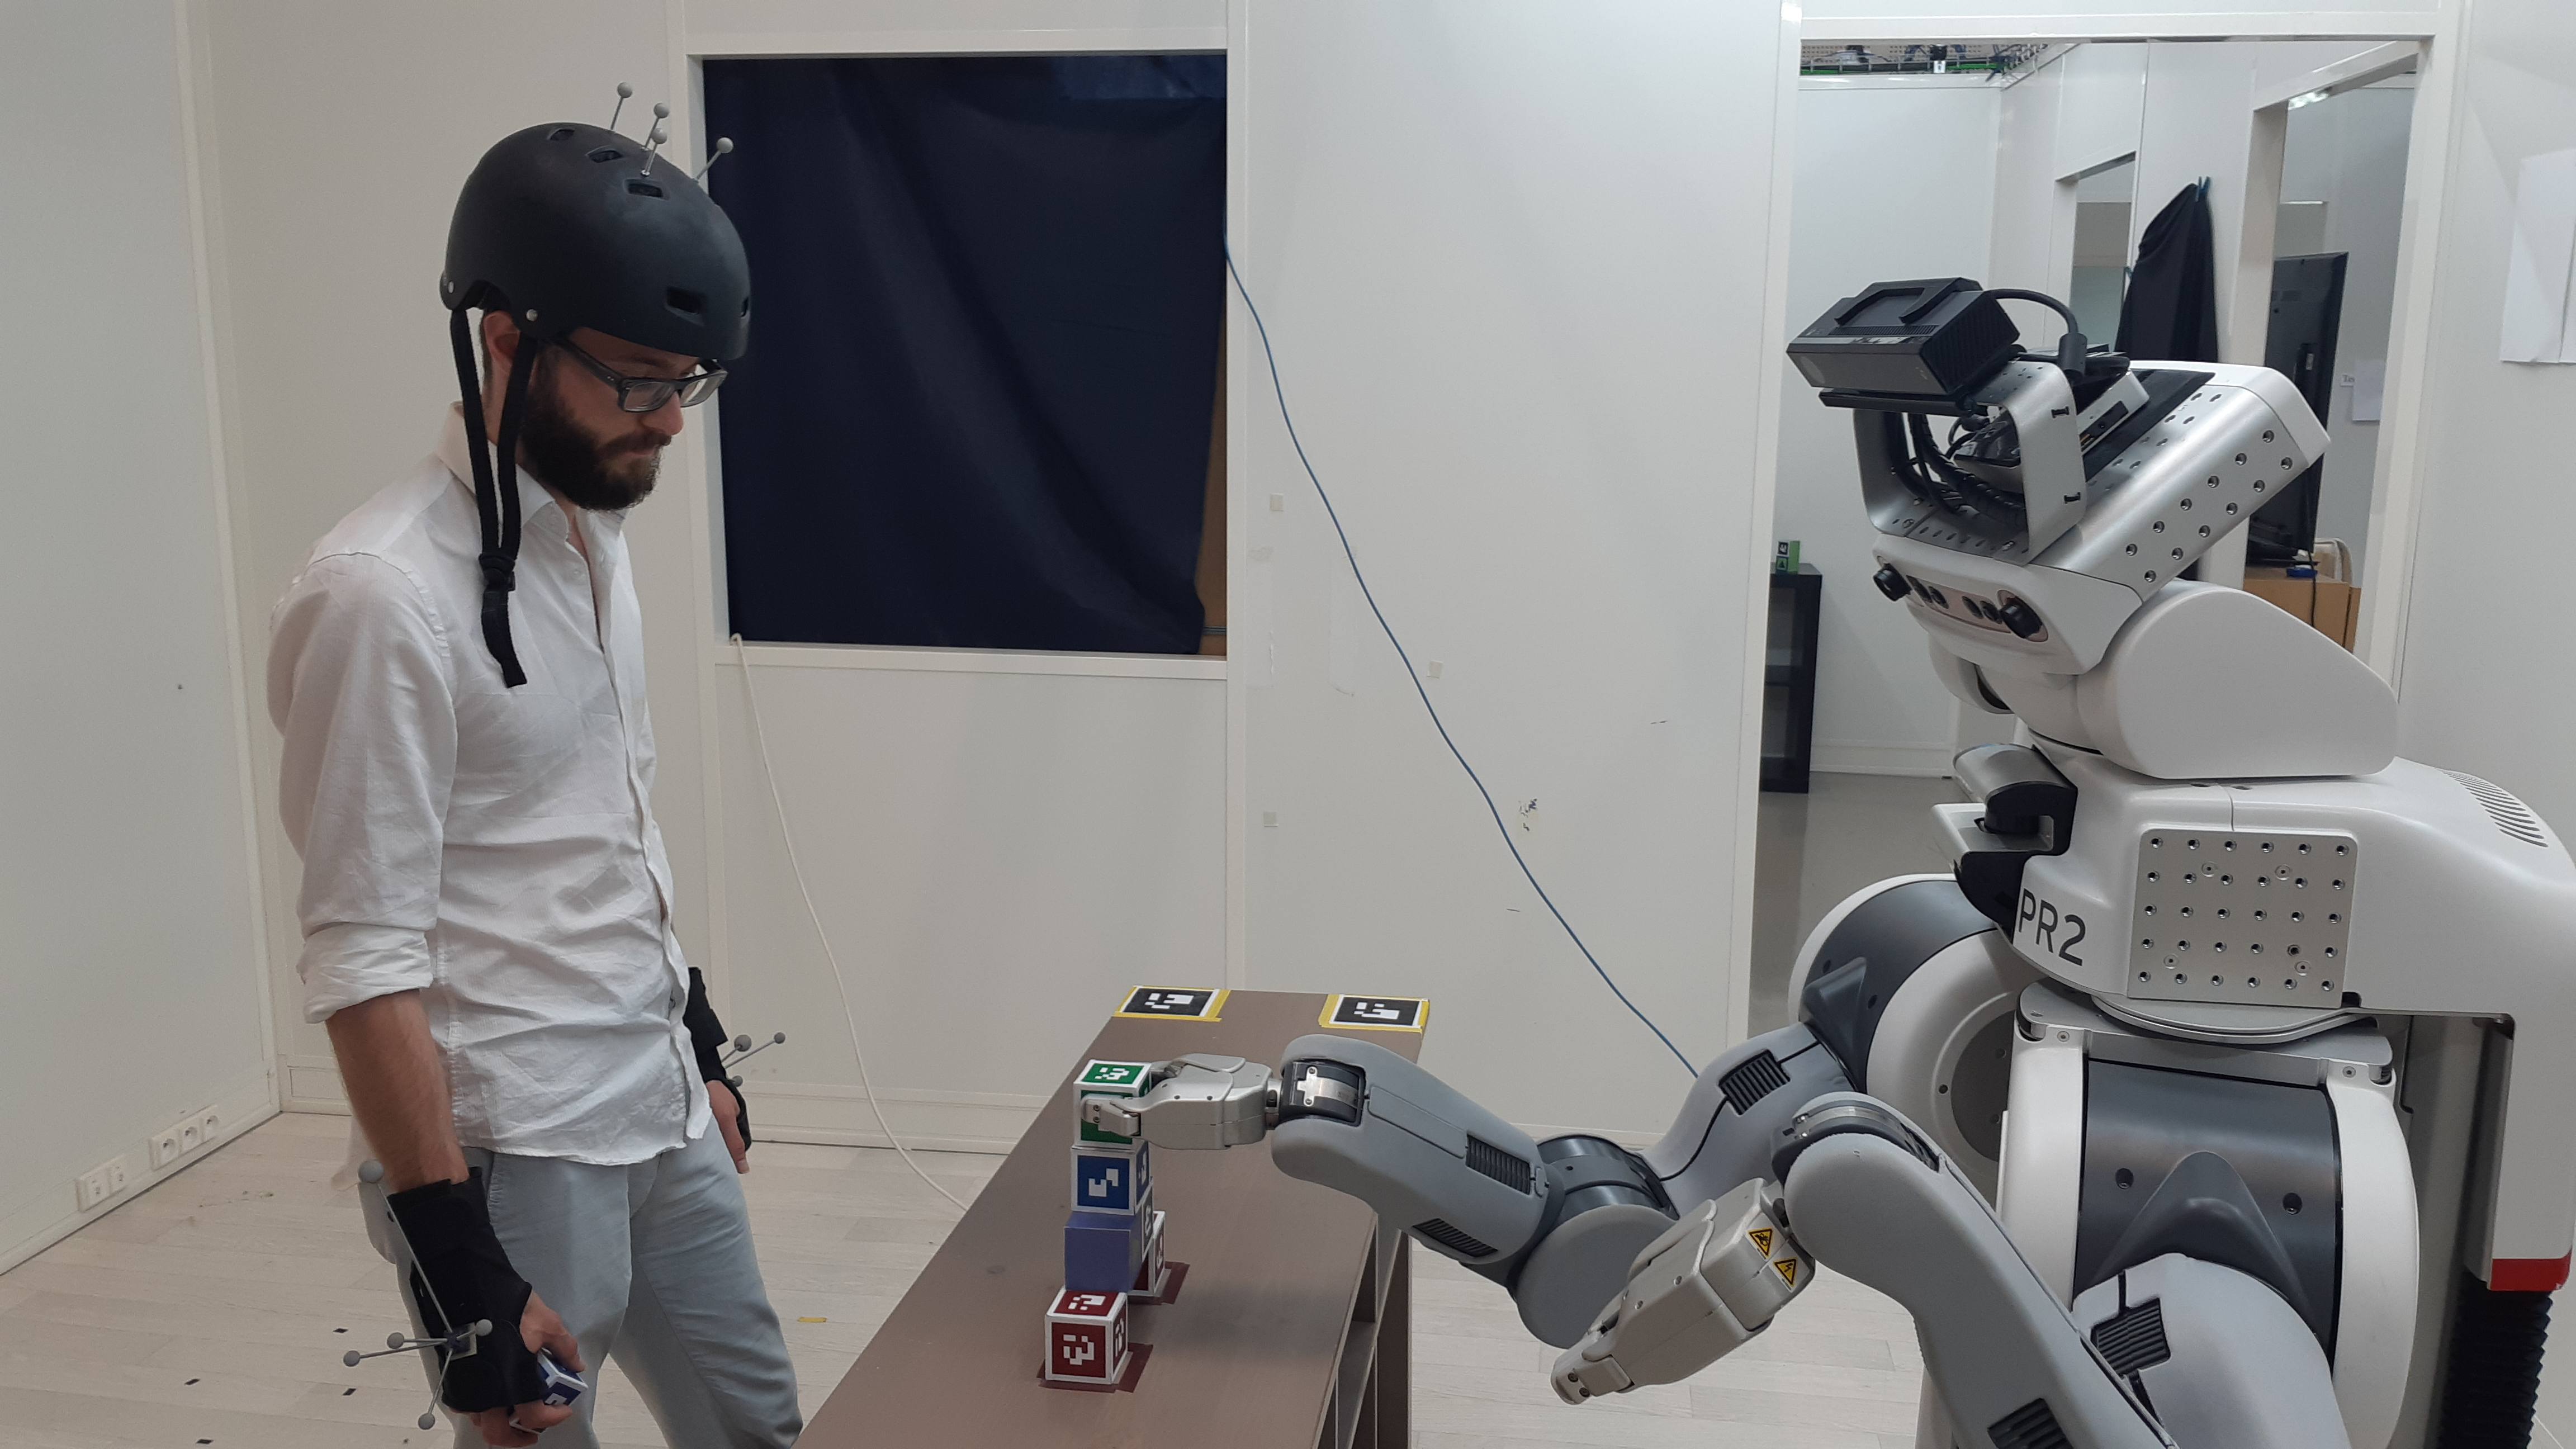
\includegraphics[width=0.7\linewidth]{figures/chapter2/building_task.jpg}
	\caption{The BuildingTask being performed by a human and a PR2 robot. The human is perceived through motion capture and the cubes with the Kinect on the robot head.}
	\label{chap6:fig:building_task}
\end{figure}

\section{Knowledge Representations and Management}\label{chap6:sec:know}
As shown in Section~\ref{chap1:subsubsec:shared_rep} and Section~\ref{chap1:subsubsec:common_g}, when involved in joint actions, humans maintain shared representations of tasks, actions, goals and have a common ground. Thus, it is important that the robot has such representations.

During an interaction, \acrshort{jahrvis} processes use knowledge bases (KB) of two types: internal and external ones. Concerning the first type, each \acrshort{rja} has its own knowledge base that we call belief base in Jason vocabulary. It is used for knowledge which serves to \acrshort{jahrvis} internal computations only. As for the external knowledge bases, there are the ones presented in Section~\ref{chap3:subsubsec:kb} as part of the robotic architecture, Ontologenius and Mementar. Updates from subscription to Ontologenius facts are received through ROS topics and converted as Jason percepts to be added to the subscribing \acrshort{rja} belief base. 

Table~\ref{chap6:tab:data} shows a description of the data circulating between the \acrshort{jahrvis} \acrshort{rja}s and the 2 \acrlong{kb}s, Ontologenius and Mementar.

\begin{landscape}
\begin{table}[]
	\centering
	\begin{tabular}{p{0.34\textwidth}||p{0.39\textwidth}|p{0.43\textwidth}|p{0.2\textwidth}|}
		
		&
		\acrshort{rja} subscription to \acrshort{kb}&
		\acrshort{rja} request/\acrshort{kb} response &
		\acrshort{rja} feeding \acrshort{kb} \\ \hline\hline
		
		\acrlong{ism} &
		\fact{isEngagedWith}{Human}{Robot}\newline
		\fact{isPerceiving}{Robot}{Human}\newline 
		\fact{isLookingAt}{Human}{Robot} &
		 &
		Start and end of interaction sessions \\ \hline
		
		\acrlong{rpm} &
		\fact{isLookingAt}{Human}{Robot} &
		Class of actions\newline SPARQL $\rightarrow$ Object &
		Start and end of abstract tasks \\ \hline
		
		\acrlong{hpm} &
		\fact{isPerceiving}{Human}{Robot}\newline \fact{isPerceiving}{Robot}{Human}\newline \fact{isLookingAt}{Human}{Robot}\newline \fact{isLookingAt}{Human}{Object} &
		Class of actions\newline Existence of action effects\newline SPARQL $\rightarrow$ Object &
		Start and end of primitive tasks \\ \hline
		
		\acrlong{cm} &
		\fact{isPerceiving}{Robot}{Human} &
		Verb conjugation\newline Class of actions and objects\newline Labels of actions and objects\newline Existence of verbalization contexts &
		\\ \hline
		
		\acrlong{ham} &
		Movements of the human action model\newline Progression effects of the human action model\newline Necessary effects of the human action model &
		Class of Objects\newline Existence of preconditions\newline Existence of isReachable(Object) &
		\\ \hline
		
		\acrlong{aem} &
		&
		Class of actions &
		Start and end of primitive tasks \\ \hline
		
	\end{tabular}
	\caption{Data circulating between the Knowledge Bases (Ontologenius and Mementar) and the \acrshort{jahrvis} \acrshort{rja}s. Data in italics are not task-dependent, the other ones are. The types of the latter are loaded from the action models described in Paragraph:~\nameref{chap6:par:act_rep}. For example, the \acrlong{ham} gets from the internal action model that \fact{handMovingToward}{Human}{Pickable} is a movement of the Pick action. Then, it can subscribe to the updates about this fact type to Ontologenius when a task where the human has a Pick action is ongoing.}
	\label{chap6:tab:data}
\end{table}
\end{landscape}

\subsection{Action Representations}\label{chap6:subsec:action_rep}
Action representations allow 
\begin{bulletList}
	\item the robot to recognize human actions
	\item to execute actions
	\item to monitor the human's attention towards its actions and to communicate about them
\end{bulletList} 

We defined three action representations according to these three uses. Actions should be written and loaded by the programmer according to the task they need the robot to perform, following the defined formats in the dedicated files. This allows \acrshort{jahrvis} core to be task-independent.

Human actions to recognize and robot actions to execute are written in an ASL file to benefit from Jason reasoning features. And, the same robot actions but with other information allowing \acrshort{jahrvis} to communicate about them and to monitor the human's attention towards them are stored in Ontologenius to benefit from the reasoning features. This latter representation is described in the next paragraph.

\paragraph{External Action Representation} (\ie stored in Ontologenius).
For the needs of \acrshort{jahrvis}, we represented actions, their verbal labels and their effects in the semantic \acrshort{kb} managed by Ontologenius. We show in Figure~\ref{chap6:fig:class_actions} a representation of some actions we stored in Ontologenius using the Web Ontology Language (OWL) (see Listing~\ref{chap2:lst:classes}) and in Figure~\ref{chap6:fig:class_effects} a representation of possible action effects.

\begin{lstlisting}[style=OwlTurtle, label={chap2:lst:classes}, caption={Description of ontology classes in the OWL language using the Turle syntax.} ]
:PhysicalAction	rdf:type owl:Class ;
				rdfs:subClassOf :HtnAction .

:PlaceAction	rdf:type owl:Class ;
			rdfs:subClassOf :PhysicalAction ;
			htn_actions:hasEffect :IsOnTopOfEffect ;
			rdfs:label ``{Agent} @Place {Pickable}'' .

\end{lstlisting}

One of the advantages of using action model stored in Ontologenius is the class inheritance. It allows to define properties for one class that will be transmitted to its child classes (\eg if it exists multiple class representing a Place action, let's say \verb'human_place_cube' and \verb'robot_place_cube', both inherit from the properties of \verb'PlaceAction' such as the label used for the action verbalization). Another advantage is to be able to link classes through properties and to easily query the \acrshort{kb} about it (\eg what are the effects of the \verb'PickAction' and then what types of effects are they?).

\begin{figure}[!ht]
	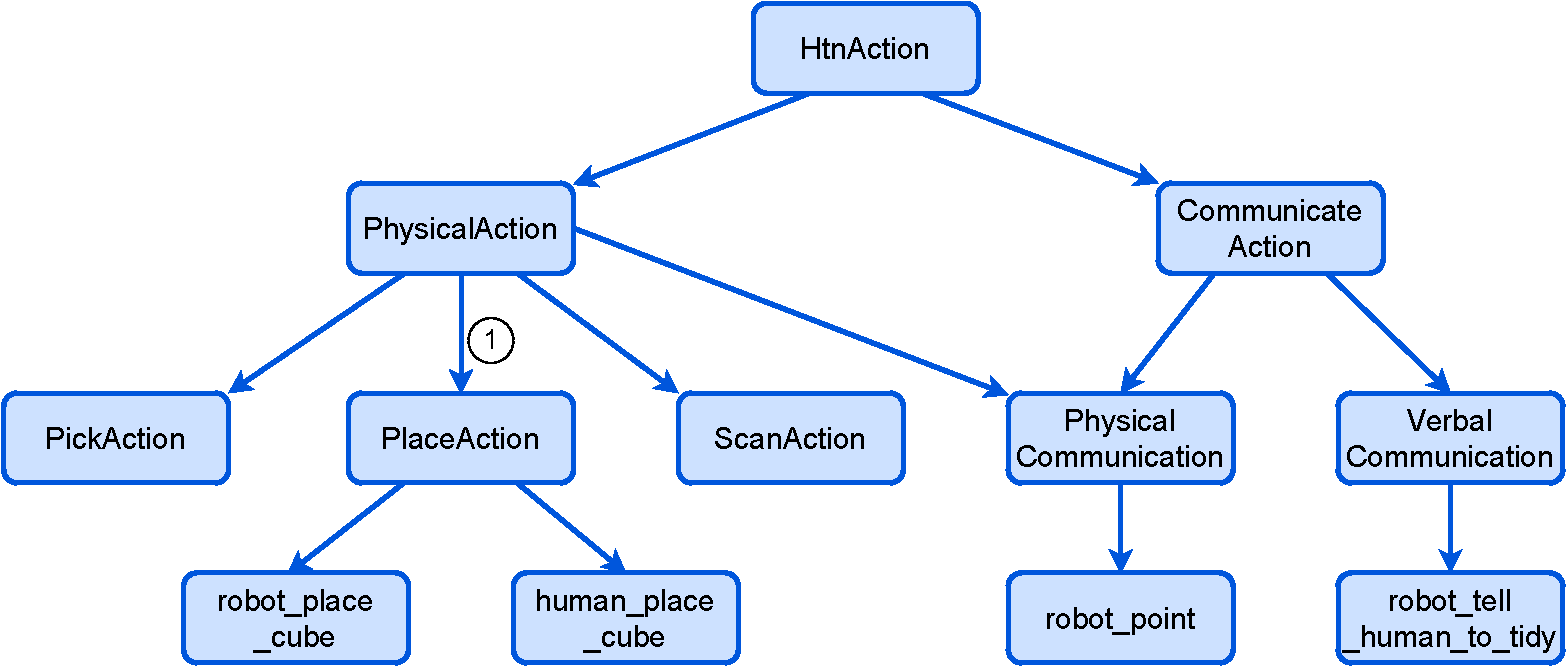
\includegraphics[width=\linewidth]{figures/chapter2/class_actions.pdf}
	\caption{The representation of an extract of the ontology class hierarchy graph of \acrshort{htn} actions. Taking the class PhysicalAction, the arrow \circledtext{1} has to be read	as \textit{``A PlaceAction is a kind of PhysicalAction''}.}
	\label{chap6:fig:class_actions}
\end{figure}

\begin{figure}[!ht]
	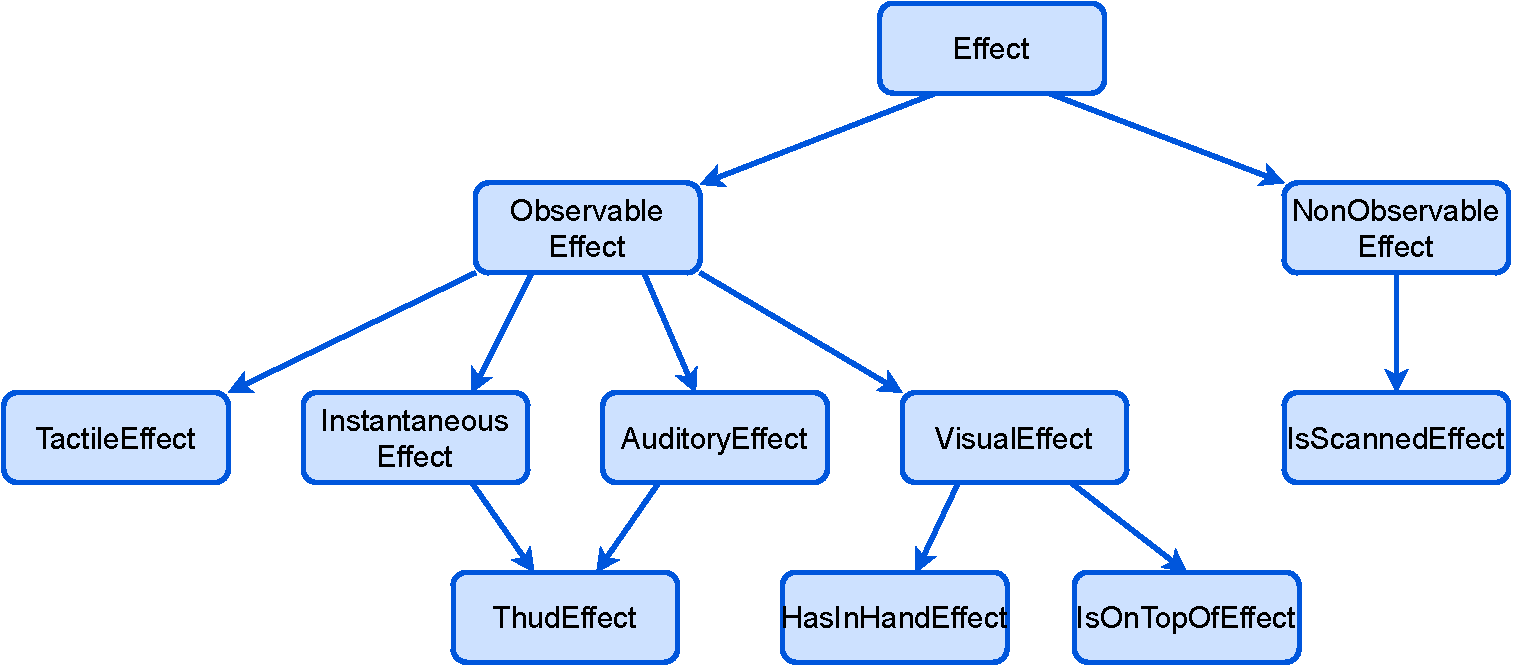
\includegraphics[width=\linewidth]{figures/chapter2/class_effects.pdf}
	\caption{The representation of an extract of the ontology class hierarchy graph of action effects. Taking the class ThudEffect, the arrows \circledtext{1} and \circledtext{2} indicate that ThudEffect is and an InstantaneousEffect and an AuditoryEffect.}
	\label{chap6:fig:class_effects}
\end{figure}

As we know, when an agent performs an action, the other agent may monitor it, if present, in order to follow the task progress and to know when the action is over. A way to know that an action is over is to check if the action effects has been added to the current worldstate or not. However, effects may be perceived differently according to the agent type as humans and robots does not have the same perception modalities (and even in one given type it can differ). In Figure~\ref{chap6:fig:class_effects}, we represented a possible way to model and classify action effects. And so, because Ontologenius is designed for \acrshort{hri}, it is possible to have different representations for robot agents and human agents. We present now a use case with its illustration in Figure~\ref{chap6:fig:kettle}. An agent may have to perform \verb'HeatWaterInKettleAction'. If it is performed by the human, the robot has to monitor the action effects to know if the action is over or not. However, a robot is not able to observe that a kettle has finished to boil water, thus the action has a non-observable effect for the robot. Then, probably the robot will ask the human if the action is over or will see that the human performs its next action of the plan. Now, if we place ourselves in the case where the robot is the one performing the action -- with a smart kettle --, it wants to check if the human could be aware of the action end (because if they are not aware, it should to inform them). The criteria \acrshort{jahrvis} takes into account is, was the effect observable by the human partner? To answer this question, it first needs to know what the observable effects of \verb'HeatWaterInKettleAction' for the human (if there are). Then, it can query the human's belief base in Ontologenius and get the knowledge that for them, the effect of \verb'HeatWaterInKettleAction' belongs to the class \verb'ThudEffect' (when the kettle stops, it produces a thud) and \verb'TactileEffect' (when the kettle boils water, it becomes hot).
	
\begin{figure}[!ht]
	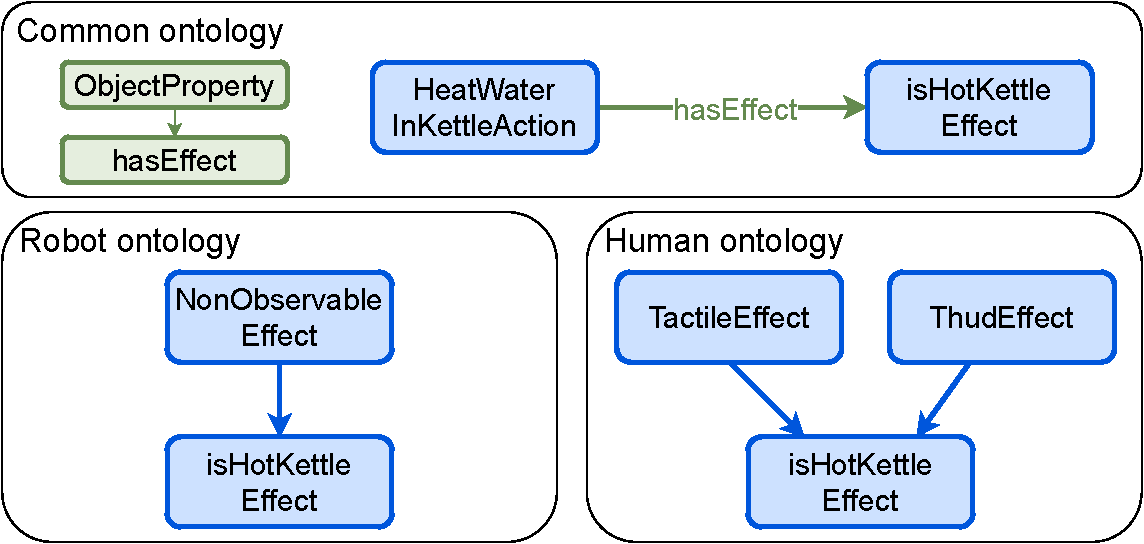
\includegraphics[width=\linewidth]{figures/chapter2/kettle.pdf}
	\caption{Illustration of the human and the robot having differing ontologies. Both have the common knowledge that HeatWaterInKettleAction has isHotKettleEffect as effect. However, in the robot ontology, isHotKettleEffect is defined as a NonObservableEffect whereas in the estimated human ontology it is defined as a TactileEffect and a ThudEffect which are both ObservableEffect as shown in Figure~\ref{chap6:fig:class_effects}.}
	\label{chap6:fig:kettle}
\end{figure}

Finally, as mentioned earlier and as visible in Listing~\ref{chap2:lst:classes}, Ontologenius allows to define label classes and so label for actions. These labels are then used by \acrshort{jahrvis} to verbalize the plan actions and based on a simple grammar we defined. For example, in ``\{Agent\} @Place \{Pickable\}'', elements between braces are to be instantiated at execution time by \acrshort{jahrvis} communication process when needed. Then, the @ symbol indicates that the word is a verb that should be conjugated. Verb conjugations can also be found in the \acrshort{kb} as shown in Listing~\ref{chap2:lst:verb}. Thus, the communication manager could process it leading to ``I placed the blue cube''.

\newpage

\begin{lstlisting}[style=OwlTurtle, label={chap2:lst:verb}, caption={Description of the class describing the verb Place in the third-person present-tense, in the OWL language using the Turle syntax.} ]
:PlaceTSPSimplePresent	rdf:type owl:Class ;
						rdfs:subClassOf :PlaceSimplePresent ;
						rdfs:subClassOf :ThirdSingularPersonalForm ;
						rdfs:label ``place''@fr ;
						rdfs:label ``places''@en .
\end{lstlisting}

We have seen the possibilities offered by Ontologenius to \acrshort{jahrvis}. Now, we present the two internal action representations, one of the human actions in order to recognize them and the other one is of the robot actions, to allow the robot to estimate the human monitoring activity of its actions. 

\paragraph{Internal Action Representation}\label{chap6:par:act_rep}(\ie stored in \acrshort{jahrvis})\mbox{}

\bigskip
What does \acrshort{jahrvis} need to \textbf{recognize a human action}? We defined a human action as: 
\[Act_H=\langle Action,PrecondL,MoveL,ProgEffectL,NecessEffectL\rangle\] where $Action$ is a predicate in the form of a triplet $ActName(Agent,Params)$ with $ActName$ the action name, $Agent$ the class of the agent performing it (\eg Human or Worker) and $Params$ a list of the action parameter classes; $PrecondL$ the list of the action preconditions; $MoveL$ the list of distinctive movements that the human could do when performing the action; $ProgEffectL$ the list of effects that we coined \textit{progression effects} which are action effects, not enough to rule the action end but allowing the plan managers to estimate that an action is progressing towards its end; and $NecessEffectL$ the list of effects that we coined \textit{necessary effects} which are action effects existing iff the action is over.

Our action model takes the form of Jason beliefs written in an ASL file, added as input of the \acrshort{rja} Human Action Monitoring. For example, the actions Pick and Place for a human are represented as:
\begin{lstlisting}[style=aslDef]
actionModel(pick(Human,[Pickable]),
			[isOnTopOf(Pickable,Support)],
			[handMovingToward(Human,PickableList)],
			[isHolding(Human,Pickable)],
			[~isOnTopOf(Pickable,Support)]).

actionModel(place(Human,[Pickable,Support]),
			[isHolding(Human,Pickable)],
			[handMovingToward(Human,SupportList)],
			[~isHolding(Human,Pickable)],
			[isOnTopOf(Pickable,Support)]).
\end{lstlisting}

The choice to have two kinds of effects has been made in order to allow the Human Action Monitoring to be robust to a potentially unreliable perception. Indeed, for example in the case of a Place action, the perception of an object hold by a human can be jumpy, and receiving the fact that the object is not in the human's hand anymore. It could reappear a few instant later. On the other, if the robot perceives that the object has been placed on top of a support, it can assume that the action is really over. The algorithm of Human Action Monitoring will be more detailed in Section~\ref{chap6:sec:h_moni}.

\bigskip

The action representation for \textbf{robot action execution} allows to match, for a given action, its name and the motion planner and executor needed to execute it. It is possible to specify how the action parameter should be fed to the motion planner and the reaction the robot should have in case of execution failure. The example given in Listing~\ref{chap6:listing:int_rep_act_exec} shows what functions of the motion planner and executor call and how the system should react in case of failure.
\begin{lstlisting}[label=chap6:listing:int_rep_act_exec,style=aslDef, frame=single, caption={Example of an internal action definition for a robot action. The first Jason plan specifies what function to call to execute the Place action. The second plan describes what should be done in case of action planning or execution failure. The third plan is triggered when the first plan has already been tried twice and was requested for a third time. In this case, the failure is signaled at the plan level.}]
// execution limited to 2 trials in a raw
@place[max_attempts(2)] 
+!place(Params) : planPick("armUsed", Arm) <-
			.nth(1, Params, Obj);
			headManager(Obj,environment_monitoring,urgent);
			planPlace(Obj, Arm);
			execute("place").
		
// in case of failure, we try again if did not already
-!place(Params)[error_msg(Msg)] : 
	not .substring(max_attempts,Msg) <-
			+error_msg(Msg);
			!place(Params).

// if we tried to execute the plan three times in a raw,
// the action is dropped	 
-!place(Params)[error_msg(Msg)] : 
	.substring(max_attempts,Msg) <-
			?error_msg(Msg);
			.fail_goal(executeAction,[error_msg(Msg)]).
\end{lstlisting}


\subsection{Shared Plan Representation}\label{chap6:subsec:shared_p_rep}
As explained in Section~\ref{chap5:sec:levels}, we represent shared plans using \acrfull{htn} as \acrshort{hatp} and \acrshort{hatpehda}, the planners we used generate \acrshort{htn}-based plans. This formalism allows to deal with goal-based and situation-based activities at different levels of hierarchy such as task, subtasks -- abstract tasks using planning vocabulary -- and actions -- atomic, primitive tasks -- and consequently to consider different levels of granularity. For example, it may be useful to \acrshort{jahrvis} to be able to request a plan for a given abstract task which failed\footnote{This is future work.}. Another advantage is that it is easy then for the robot to communicate about subtasks and not only about actions without context. However, according to the task or the domain, the \acrshort{htn} expressiveness for this matter raises discussion. Indeed, \acrshort{htn} plans often make use of recursive abstract tasks which becomes useless for replanning because such abstract tasks have no semantic meaning. Indeed, if we take the piece of plan presented in Figure~\ref{chap6:fig:recursive_task}, to communicate to the human that the abstract task PlaceAllObjects has failed does not give a information precise enough since there are several of them.

\begin{figure}[!ht]
	\centering
	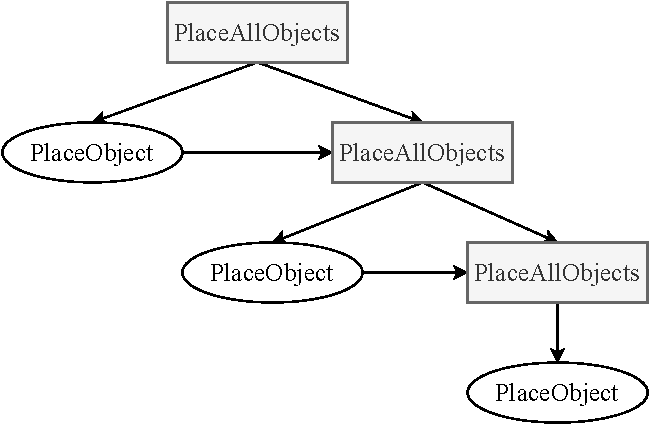
\includegraphics[width=0.6\linewidth]{figures/chapter2/recursive_task.pdf}
	\caption{Example of a recursive abstract task. The white ellipses correspond to primitive tasks while gray rectangles represent abstract ones.}
	\label{chap6:fig:recursive_task}
\end{figure}

Moreover, in the next section (see~\ref{chap6:subsec:feeding}), we show how \acrshort{jahrvis} feeds the episodic ontology, a timeline, with abstract and primitive task executions. It becomes humanly unreadable with recursive tasks. A concept such as the ``iterative task'' proposed by Martinie \etal{}~\cite{martinie_2011_structuring} would be interesting if used in a \acrshort{htn} plan for \acrshort{hri}. However, there is currently no such thing, so when manipulating such plans we have two modalities:
\begin{enumerate}
	\item the domain is written being aware of this issue and thus, \acrshort{jahrvis} takes abstract tasks as input besides primitive tasks (\ie in the current work, plans generated by \acrshort{hatpehda}\footnote{Based on domains intentionally written without recursive tasks by Guilhem Buisan.})
	\item the domain is written with recursive abstract tasks and thus, \acrshort{jahrvis} only selects primitive tasks as tasks being part of the plan (\ie in the current work, plans generated by \acrshort{hatp}\footnote{Reuse of domains written by Sandra Devin.})
\end{enumerate}

We define a shared plan as a sequence of primitive tasks having to be performed by an agent and, abstract tasks. An abstract task $\lambda$ is defined as: 
\[\lambda=\langle id_\lambda,state_\lambda,name_\lambda,\Delta_\lambda\rangle\] 
where $id_\lambda$ is an identification number (id) proper to $\lambda$, $state_\lambda$ is the task state estimated by the robot, $name_\lambda$ is the name of the task and the decomposition id $\Delta_\lambda=id_{\lambda\prime}$ with $id_{\lambda\prime}$ the id of the abstract task $\lambda\prime$ that has been decomposed into other tasks, including $\lambda$.

And, a primitive task $\Pi$ is defined as:
\[\Pi=\langle id_\Pi,state_\Pi,name_\Pi,agent_\Pi,params_\Pi,preds_\Pi,\Delta_\Pi\rangle\]

where $id_\Pi$ is an id proper to $\Pi$, $state_\Pi$ is the task state estimation by the robot, $name_\Pi$ is the name of the task, $agent_\Pi$ is the name of the agent that should perform the task, $,params_\Pi$ is the list of parameters required for the task execution, $preds_\Pi={id_{\Pi\prime},...,id_{\Pi\prime\prime}}$ the list of ids of the tasks $\Pi\prime,...,\Pi\prime\prime$ needing to be achieved before the task $\Pi$ can start, and the decomposition id $\Delta_\Pi=id_{\lambda}$ with $id_{\lambda}$ the id of the abstract task $\lambda$ that has been decomposed into other tasks, including $\Pi$.

We defined nine possible values for an abstract or primitive task $state$ which are shown in Table~\ref{chap6:tab:task_states}. 

\begin{table}[h]
	\centering
	\begin{tabular}{l|l}
		State            & Description         \\\hline\hline
		\textsc{planned} & needs to be done later        \\
		\textsc{todo}            & needs to be done now   \\
		\textsc{ongoing}          & is in progress       \\
		\textsc{executed}         & is achieved               \\
		\textsc{suspended}        & needs to be set to \textsc{unplanned}\\ 
		\textsc{unplanned} & is not part of the plan anymore (used with conditional plans) \\
		\textsc{not\_starting}    & was \textsc{todo} but took to much time before starting \\
		\textsc{not\_finished}     & was started but has not been achieved    \\
		\textsc{not\_seen}         & was achieved but has not been observed by the other agent    
	\end{tabular}
	\caption{The nine possible state values of an abstract or primitive task.}
	\label{chap6:tab:task_states}
\end{table}

So, for example, an excerpt of the BuildingTask plan in which the human and the robot place the first blue cube of the stack and the green cube, generated by \acrshort{hatpehda} and represented in Figure~\ref{chap6:fig:excerpt_plan}, is:
\thispagestyle{example}
\begin{align*}
&\lambda_{13}=\langle 13,\textsc{Planned},\text{h\_place\_blue\_cube},1\rangle \\
&\lambda_{4}=\langle 4,\textsc{Planned},\text{r\_place\_green\_cube},1\rangle \\
&\Pi_{139}=\langle 139,\textsc{Planned},\text{human\_place\_cube},\text{human\_0}, [\text{blue\_cube\_2,stick}],138,13\rangle \\
&\Pi_{141}=\langle 141,\textsc{Planned},\text{robot\_place\_cube},\text{pr2\_robot},[\text{green\_cube,blue\_cube\_2}], &\\  & &139,4\rangle
\end{align*}\todo{arrange}

\begin{figure}[!ht]
	\centering
	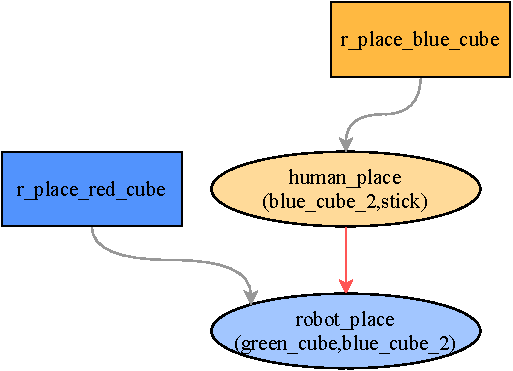
\includegraphics[width=0.5\linewidth]{figures/chapter2/excerpt_plan.pdf}
	\caption{An excerpt of the BuildingTask plan. The ellipses correspond to primitive tasks while rectangles represent abstract ones. The blue shapes are robot tasks and the yellow ones are the human ones. Finally, red arrows indicate the sequence of actions in the plans and gray ones represent hierarchical links, \textit{i.e.}~the links between the tasks as defined in the \acrshortpl{htn}.}
	\label{chap6:fig:excerpt_plan}
\end{figure}

\subsection{Feeding the Knowledge Base}\label{chap6:subsec:feeding}
Until now, we stayed focused on semantic knowledge going from the external \acrshort{kb} to \acrshort{jahrvis}. But, as mentioned earlier, one of the external \acrshort{kb} is dedicated to episodic knowledge. This \acrshort{kb} takes the form of a timeline, managed by Mementar. Whereas Ontologius feeds \acrshort{jahrvis} with knowledge, the flow is inverted for the episodic data, as Mementar is fed by \acrshort{jahrvis} among other components. Indeed, when an abstract or primitive task is started or achieved, this information is sent to Mementar for storage with the associated ID and time stamp. The objective is to have a history of the task proceeding. One of the possible use of such a history is for the robot to refer to past events during a task when communicating.
Moreover, \acrshort{jahrvis} adds the semantic data associated to a task -- agent and parameters -- to the semantic ontology. 
%We illustrate the timeline in Figure~\ref{chap6:fig:timeline} with the same example as the one above for the plan, one cube is placed by each agent.


%\begin{figure}[!ht]
%	\includegraphics[width=\linewidth]{figures/chapter2/timeline.png}
%	\caption{Piece of timeline of an executed BuildingTask plan where the robot and the human had to place a cube each. It has been generated by Mementar after having received data from \acrshort{jahrvis}.}
%	\label{chap6:fig:timeline}
%\end{figure}\todo{refaire et ajouter le temps en legende}


\thispagestyle{example}

\section{Interaction Session Management} 

\begin{figure}[!htb]
	\centering
	\includegraphics[width=0.7\linewidth]{figures/chapter2/session_manager_zoom.pdf}
	\caption{The \acrlong{ism} and the \acrshort{rja}s (in blue) and the component of the robotic architecture (in red) with which it interacts.}
	\label{chap6:fig:session_manager_zoom}
\end{figure}

The \acrfull{ism} handles the interaction sessions and manages the robot (shared) goals. Figure~\ref{chap6:fig:session_manager_zoom} proposes a focus on the \acrshort{jahrvis} structure and the components of the robotic architecture around the \acrshort{ism}. Figure~\ref{chap6:fig:session_manager} shows the process we designed, modeling the different states in which the robot can be. Moreover, we thought the manager with the ability to consider that a human can join another one during a conversation. However, we have not implemented it yet.

\begin{figure}[!htb]
	\centering
	\includegraphics[width=0.8\linewidth]{figures/chapter2/session_manager.pdf}
	\caption{States of the \acrfull{ism}. In blue are represented the states of the \acrshort{ism} when the robot is not in an interaction session. In orange are the states in which the \acrshort{ism} can be during an interaction session. In green are the sub-states of the interaction session body.}
	\label{chap6:fig:session_manager}
\end{figure}

A simpler version work as following. An interaction session is triggered when a human is close enough to start a conversation and seems willing to, \ie when the fact  \fact{isEngagedWith}{human\_i}{robot} is added to the knowledge base and sent to \acrshort{jahrvis}. In this way, the robot tries to respect people that does not want to interact with it. From there, the robot is in the first phase of the interaction session, the \textit{greetings}. The robot says hello to the human and announces the activities it can perform with them, depending on the context they are in. The interaction manager triggers the tracking of the human's head by the robot head. This has two purposes: to signal the robot's engagement and to monitor the human's actions. This behavior is quite similar to the one described by Satake \etal~\cite{satake_2015_should}. 


An interaction session stays open as long as the human and the robot perform activities together, \ie as long as the human is engaged in the interaction. This engagement is monitored by the robot in different ways: through the predicate \fact{isEngagedWith}{human\_i}{robot} during dialogue phases outside a task and through what is happening during a task. If at some point the human is not perceived for a while or the human says goodbye, then the manager ends the session. In the latter case, the robot replies with goodbyes. Finally, it returns to its home-base if it has one.

\section{Human Actions Recognition}\label{chap6:sec:h_moni}
\begin{figure}[!hbt]
	\centering
	\includegraphics[width=0.8\linewidth]{figures/chapter2/action_reco_zoom.pdf}
	\caption{The \acrlong{ham} and the \acrshort{rja}s (in blue) and the component of the robotic architecture (in red) with which it interacts. It is fed by a file (in white) with description of the human actions the robot should recognize.}
	\label{chap6:fig:action_monitoring_zoom}
\end{figure}

In order to coordinate properly, humans monitor each others when they are in a joint action (see Section~\ref{chap1:subsubsec:monitoring}). The robot needs the same kind of process to be able to assess if the human is doing the action of the plan it expects or not. This allows to follow the plan progress and to estimate the level of human engagement. Existing solutions exist to recognize human actions but none of them matched all our criteria which are: \todo{faire un état de l'art rapide}
\begin{bulletList}
	\item it should be easy and quick to add a new action that the robot can recognize
	\item the process should output the action parameters
	\item the process should give information about the action progress, \ie modeling the action start and progression when possible and not only the end
	\item it needs to be robust to a potentially unreliable perception
	\item an available open-source code 
\end{bulletList}

Thus, we implemented our own model-based solution with an \acrshort{rja} dedicated to \acrfull{ham}. Figure~\ref{chap6:fig:action_monitoring_zoom} shows its relations with the other \acrshort{rja} of \acrshort{jahrvis}  and components of the robotic architectures. It could be replaced later with a more complex solution meeting the needs, but even though the current one is quite simple, it has interesting properties, matching the criteria presented above.

The \acrshort{ham} relies on the action model presented in Section~\ref{chap6:par:act_rep} which it loads at initiation. We chose to base our action recognition process on human movements and action effects that the robot can observe. As it needs to recognize them, it extracts the predicate types corresponding to those and subscribes to updates about these facts to Ontologenius as explained in Section~\ref{chap6:sec:know}. 

Continuously, the \acrshort{ham} \acrshort{rja} receives facts and human movements that are present in the action model, and sends to the \acrfull{hpm} \acrshort{rja} three types data about human actions: 
\begin{bulletList}
	\item list of actions that may have started that we coined \emph{possibly started actions}
	\item list of actions that may be progressing that we coined \emph{possibly progressing actions}
	\item list of actions that are estimated as finished that we coined \emph{possibly achieved actions} 
\end{bulletList}

\begin{figure}[!hbt]
	\includegraphics[width=\linewidth]{figures/chapter2/action_sm.pdf}
	\caption{Representation of the \acrfull{ham} \acrshort{rja} in the form of a Finite State Machine representing the state of one action. Transitions are composed of a triggering event (+Fact or -Fact) and a condition between square brackets. Variable names ending with a ``L'' are list of effects, either the necessary effect list of a given action in the model (actionNecessEffectL) or the list of facts in the current worldstate corresponding to the effects of a given action (matchedNecessEffectL).}
	\label{chap6:fig:action_monitoring}
\end{figure}

Action states are updated according to the facts defined in the human action model that the \acrshort{ham} receives. When the state of an action changes to \emph{possibly started}, \emph{possibly progressing} or \emph{possibly achieved}, the affected list is updated and sent to the \acrshort{hpm}. 

We chose to use the term \emph{possibly} to describe these states as it is well-known that some estimations of action states are false but they allow the system to have an idea of what might be going on.

The algorithm we developed can be depicted in the form of a Finite State Machine representing the state of one action as shown in Figure~\ref{chap6:fig:action_monitoring} and is implemented in ASL (the code is available in Appendix~\ref{app:jahrvis:h_monitoring}). Many State Machines can run simultaneously, one for each action that is estimated to be in one of the states. The parameters field of an action are filled as it is making progress through the states, according to the movement and effects allocated to this action.


\thispagestyle{example}

Each transition is triggered by the addition or the deletion of a fact. Using Jason rules\footnote{They are quite similar to Prolog rules.}, facts are analyzed to see if they match a movement or an effect of a known action. For example, if we look at the Place action example presented in Section~\ref{chap6:par:act_rep}, when performed by a human, it expects the fact \fact{handMovingToward}{Human}{Support} as a movement. Therefore, receiving \fact{rightHandMovingToward}{human\_0}{placement\_1} will match a Place action movement and will add the action to the list of \emph{possibly started actions}. However, receiving \fact{rightHandMovingToward}{human\_0}{phone} will not, as the phone does not belong to the Support class (but this fact may be useful for recognizing another action).
 
It is not shown on the Figure for clarity reasons, but each state, except \emph{possibly achieved}, has a transition to the final state which is triggered by a time deadline. Currently, this timeout is the same for each action but as every action type might be of different lasting, a deadline could be specifically set for each one. All the other transitions of the state machine are described in Table~\ref{chap6:tab:action_monitoring}.


\newgeometry{left=1in,right=1in,top=1in,bottom=0.5in,includefoot,includehead,headheight=13.6pt}

\begin{landscape}
%	\vspace*{\fill}
	\begin{table}[htb!]
	\caption{Description of the Finite State Machine shown in Figure~\ref{chap6:fig:action_monitoring}. Inputs are triggering events (+Fact or -Fact) and conditions are between square brackets. Variable names ending with a ``L'' are list of effects, either the necessary effect list of a given action in the model (actionNecessEffectL) or the list of facts in the current worldstate corresponding to the effects of a given action (matchedNecessEffectL).}
	\label{chap6:tab:action_monitoring}
	\begin{tabularx}{\linewidth}{| c | c | c | X |}
		Current State & Input and Condition & Next State & Explanation\\ 
		\hline \hline
	\multirow{4}{*}{Initial State}  & +Fact [matchActionMovement(Fact)] & Possibly Started & When a fact matching a movement and filling the preconditions for a given action is received, \acrshort{ham} computes that the human may have initiated an action. \\  
		\cline{2-4}
		&  \makecell{+Fact [matchNecessEffect(Fact) 
			\\ \&\& length(actionNecessEffectL)	== 1
			\\ \&\& possibleActorExists]} & Possibly Achieved & The robot may have missed the movement or the progression effect of an action because it was not looking or the perception did not detect it. Then when a necessary effect is received and that only one exists for the action, the action is estimated as achieved if it is possible to find an agent who may have performed it. For now, the finding function is looking for humans in the vicinity of the effect objects, and if there are several humans, it selects the closest one.\\  
		\cline{2-4}
		&  \makecell{+Fact [matchNecessEffect(Fact) 
		\\ \&\& length(matchedNecessEffectL)
		\\ < length(actionNecessEffectL)
		\\ \&\& possibleActorExists
		\\ || matchProgEffect(Fact)]} & Possibly Progressing & Similarly to the case above, the robot may have missed the movement or the progression effect of an action. However, if this action has several necessary effects, the action is considered as progressing.\\  
		\cline{2-4}
		& \makecell{+Fact [matchRobotAction(Fact)
		\\ || matchEffect(Fact) \&\& !possibleActorExists]} & Final State & The \acrshort{ham} is aware of the actions executing by the robot so it does not mismatched its action effects with the ones of another agent. If an effect matches, nothing happen. Likewise if an effect is detected but no agent could be found that might have done it.\\  
		\hline 
	\end{tabularx}
\end{table}
\vspace*{\fill}
 \begin{table}[htb!]
 	\caption*{Table~\ref{chap6:tab:action_monitoring}: (continued)}
	\begin{tabularx}{\linewidth}{| c | c | c | X |}
		Current State & Input and Condition & Next State & Explanation\\ 
		\hline \hline
		\multirow{3}{*}{Possibly Started}  
		& \makecell{+Fact [matchProgEffect(Fact)
			\\ || matchNecessEffect(Fact) 
			\\ \&\& length(actionNecessEffectL) > 1]} & Possibly Progressing & When a fact corresponding to a progression effect of the started action is received, or it matches a necessary effect but there are more than one for this action, \acrshort{ham} reinforces its estimation that this action is ongoing by setting it to the progressing state.\\  
		\cline{2-4}
		& \makecell{+Fact [matchNecessEffect(Fact) 
			\\ \&\& length(matchedNecessEffectL) == 1]} & Possibly Achieved 
		& When a fact corresponding to a necessary effect is received and that there is only one for the started action, the action is considered as achieved as the robot is able to observe its effect and that it had observed the human starting it.\\  
		\cline{2-4}
		& -Fact	[matchActionMovement(Fact)] & On Probation & When a movement fact is removed from the belief base without having observed an effect, it might mean that it was a human hesitation or a false estimation and that the action is not starting. However, it might also be the robot perception being sporadic and so the action goes in this temporary state waiting for a potential coming effect.\\  
		\hline
	\end{tabularx}
\end{table}
\vspace*{\fill}
  \begin{table}[htb!]
  	\caption*{Table~\ref{chap6:tab:action_monitoring}: (continued)}
	\begin{tabularx}{\linewidth}{| c | c | c | X |}
		Current State & Input and Condition & Next State & Explanation\\ 
		\hline \hline
		\multirow{2}{*}{On Probation} 
		& \makecell{+Fact [matchProgEffect(Fact)
			\\ || matchNecessEffect(Fact)
			\\ \&\& length(actionNecessEffectL) > 1]} & Possibly Progressing & An effect is detected and the action state is resumed.\\
		\cline{2-4}
		& \makecell{+Fact [matchNecessEffect(Fact) 
			\\ \&\& length(matchedNecessEffectL) == 1]} & Possibly Achieved 
		& A necessary effect is detected and as there is only one for this action, it is considered as achieved.\\
		\hline
		\multirow{2}{*}{Possibly Progressing} 
		& \makecell{+Fact [matchNecessEffect(Fact) 
			\\ \&\& length(matchedNecessEffectL)
			\\ == length(actionNecessEffectL)]} & Possibly Achieved 
		& An necessary effect is received and in total, for this action, there was as many necessary effects received as the ones defined for this action.\\
		\cline{2-4}
		& \makecell{+Fact [matchEffect(Fact) 
			\\ \&\& length(matchedNecessEffectL)
			\\ < length(actionNecessEffectL)]} & Possibly Progressing 
		& When an action effect is received and that either it is another progressing or not the last necessary effect expected for the action, the action state remains progressing.\\  
		\hline
		Possibly Achieved & -- & Final State & When an action is estimated as achieved, this is its final state.\\
		\hline
	\end{tabularx}
	
\end{table}
\vspace*{\fill}
\end{landscape}

\restoregeometry

When the software starts, the \acrshort{ham} extracts from the internal action representation presented in Section~\ref{chap6:subsec:action_rep}, all the types of facts that should be monitored. Then, it queries Ontologenius to send it each updates about these facts. Thus, when the robot designers decide that a new action should be recognized by the robot, the only thing to add is the action model in \acrshort{jahrvis} belief base.

Moreover, sometimes new facts are actually effects of robot actions. In order to avoid that robot actions are mistaken for human ones, the \acrshort{aem} signals to the \acrlong{ham} when the robot executes a given action of the plan. 

Finally, all the functions to check if a new fact update matches an action effect are Jason rules. They rely on the external knowledge base, here Ontologenius, as there is a need to compare the predicate object and subject expected classes of an action effect with the received ones.

\thispagestyle{example}
\subsection*{Examples}
Now, we give an insight of what happens in the system when the human perform pick and place actions, based on the BuildingTask example. We will present several cases in pictures and one completed with a timeline and a sequence diagram.

\begin{figure}[!htp]
	\subfloat[The human has his hand moving toward the blue cube and the stick (the longer blue cube ).]{\label{chap6:fig:action_monitoring_photos_toward}\includegraphics[width=0.3\linewidth]{figures/chapter2/moving_toward.jpg}}\hfill
	\subfloat[The human is holding the stick.]{\label{chap6:fig:action_monitoring_photos_holding}\includegraphics[width=0.3\linewidth]{figures/chapter2/holding_stick.jpg}}\hfill
	\subfloat[The human picked the stick, it is not of top of the table anymore.]{\label{chap6:fig:action_monitoring_photos_not_top}\includegraphics[width=0.3\linewidth]{figures/chapter2/not_top_stick.jpg}}\hfill
	\caption{Decomposition of a pick action of the stick.}
	\label{chap6:fig:action_monitoring_photos_pick}
\end{figure}

\paragraph{The human has to pick the stick} 

There are two cubes on the human side: the stick and the blue cube. Both red cubes are on their placements so this is the moment where the human should pick the stick. Figure~\ref{chap6:fig:action_reco_ex1_timeline} is a timeline showing on the right the facts arrived from the situation assessment, fed to the \acrshort{kb}, and then sent to the \acrshort{ham}. First, the human starts to move his hand towards the table and the cubes (Figure~\ref{chap6:fig:action_monitoring_photos_toward}). No fact is received by the \acrshort{ham} about the table as it has subscribed to \fact{handMovingToward}{Human}{Pickable} and the table is not a Pickable. We can notice that the received facts are with the predicate \textit{rightHandMovingToward} which is a subproperty of \textit{handMovingToward}. Thus, as we can see in Figure~\ref{chap6:fig:action_reco_ex1}, it triggers the possible start of two pick actions, one for the stick and the other one for the blue cube. Then, the human has the stick in his hand but it is still on the table (Figure~\ref{chap6:fig:action_monitoring_photos_holding}), thus the pick action with the stick is considered as possibly progressing and the pick action with the blue cube remains as possibly started. Finally, the human withdraws his hand, holding the stick and so the stick is not on the table anymore (Figure~\ref{chap6:fig:action_monitoring_photos_not_top}). Therefore, the action is estimated as possibly achieved. As it was the one expected to be the next action to perform, the \acrlong{hpm} left aside the started action with the blue cube and selected the one with the stick as the one that was ongoing. It fed Ontologenius with the action and its associated parameters and Mementar with the start and end times as we can see in Figure~\ref{chap6:fig:action_reco_ex1_timeline}.

\paragraph{The human picks the blue cube while the robot is not looking} as it is picking the green cube as shown in Figure~\ref{chap6:fig:action_monitoring_photos_not_looking}. Then, as it places its cube on the stack (Figure~\ref{chap6:fig:action_monitoring_photos_now_looking}), it looks in the direction of the blue cube former position. Thus, the Situation Assessment produces the deletion of the fact \fact{isOnTopOf}{blue\_cube\_2}{table\_1} which is signaled to the \acrshort{kb}s which information is sent to the \acrshort{ham}. Then, the \acrshort{ham} evaluates if a human agent could be at the origin of this change in the environment, associated to a pick action according to the human action model. And, the answer is yes and a pick action of the blue cube is allocated to the present human.
\thispagestyle{example}
\begin{figure}[!hbtp]
	\subfloat[The human is picking the blue cube while the robot is not looking as it is picking the green cube.]{\label{chap6:fig:action_monitoring_photos_not_looking}\includegraphics[width=0.45\linewidth]{figures/chapter2/looking_somewhere_else.jpg}}\hfill
	\subfloat[The robot is looking again in the human direction and observes that the blue cube is not on the table anymore. It deduces that the human has taken it.]{\label{chap6:fig:action_monitoring_photos_now_looking}\includegraphics[width=0.45\linewidth]{figures/chapter2/now_looking.jpg}}\hfill
	\caption{The robot does not see the human picking the blue cube but then it deduces that he is the one to have performed the action.}
	\label{chap6:fig:action_monitoring_photos_missing}
\end{figure}
	
\newgeometry{left=0.9in,right=0.9in,top=1.1in,bottom=0.5in}
\begin{landscape}
	\begin{figure}[!htb]
		\centering
		\includegraphics[width=0.9\linewidth]{figures/chapter2/action_reco_1.pdf}
		\caption{Timeline produced by Mementar on which appear facts from perception (blue, on the right) and the action added by the \acrlong{hpm} based on data from the \acrlong{ham} (orange, on the left). Numbers on the axis are time in milliseconds (epoch time).}
		\label{chap6:fig:action_reco_ex1_timeline}
	\end{figure}
	
	\begin{figure}[!htb]
		\centering
		\includegraphics[width=0.75\linewidth]{figures/chapter2/action_monitoring_ex1.pdf}
		\caption{Sequence diagram for a pick action. The \acrshort{kb}s sends to the \acrshort{ham} the perceived facts to which the \acrshort{ham} subscribed. The \acrshort{ham} processes these facts through State Machines as presented above. Then it output action states which are sent to the \acrfull{hpm}. Arrows from the \acrshort{ham} to the \acrshort{hpm} of the same color (except black) than a arrow going from the \acrshort{kb}s to the \acrshort{ham} are triggered by it. A green plus sign means that it is a belief addition in the \acrshort{rja}, a red minus sign means that it is a belief deletion.}
		\label{chap6:fig:action_reco_ex1}
	\end{figure}
\end{landscape}
\restoregeometry

\section{Shared Plans Handling}\label{chap6:sec:plan_handling}
In order to correctly perform collaborative tasks with humans, the robot needs to know how to perform them. One way is to have a planner with a domain, computing a plan at execution time based on its current knowledge about the environment and interaction. Then, the robot must be endowed with a way to manage the execution of this ``recipe''. As we place ourselves in the context of joint action, plans manipulated by the robot are shared plans, as presented in Section~\ref{chap6:subsec:shared_p_rep} (to differentiate from the ASL plans presented in Section~\ref{chap4:subsec:jason} which code all the \acrshort{rja}). We make the assumption that the human knows how to create their own plan in order to reach the shared goal. So, we consider it is not necessary to verbalize it from the outset.

We claim that the robot ability to handle and execute shared plan is enhanced when endowed with \acrfull{tom} (see Sections~\ref{chap1:sec:tom} and~\ref{chap2:subsec:tom_hri}), as shown by Devin~\cite{devin_2016_implemented}. It allows the robot to be aware of false beliefs or belief divergences in the human's point of view. When such things happen, it can react appropriately, either by acting or communicating. We gave the robot such an ability\footnote{The robot has a first-order \acrshort{tom}, it estimates the human knowledge about the task but it does not compute what the human thinks of the robot knowledge about the task (second-order \acrshort{tom})}, \textit{via} two processes: the \acrfull{rpm} and the \acrfull{hpm} (see Figure~\ref{chap5:fig:sup_overview}). Therefore, the first one handles the robot's beliefs about the plan and the action execution while the second handles the estimation of the human's beliefs about the plan and the communication with the human. The \acrshort{rja}s implementing these processes are presented in Sections~\ref{chap6:subsec:robot_plan} and~\ref{chap6:subsec:human_plan}.

As we designed \acrshort{jahrvis} to be as generic as possible, it can manage different kinds of human-robot plans as input: 
\begin{bulletList}
	\item shared plans in which each action is allocated to an agent as well as action parameters are given objects,
	\item shared plans in which actions might not be allocated to an agent at planning time and parameters might refer to objects with a semantic query, and
	\item conditional plans which anticipate different possibilities for the human decision/action. 
\end{bulletList} 

To generate these plans, we worked with two planners, \acrshort{hatp} and \acrshort{hatpehda} presented in Section~\ref{chap3:subsubsec:task_planner}.

\paragraph{``Usual'' shared plans with HATP and HATP/EHDA} The first type of shared plans handled are what we could call ``usual'' shared plans. Each action is allocated to an agent as well as action parameters are given objects. Thus, in this kind of plan, no decision is left to \acrshort{jahrvis} about who should execute the action or with what object.

\paragraph{AgentX shared plans with HATP}
The second type of shared plans is an extension of the work of Devin about postponing some decisions from planning time to execution time about the actor of some actions and some parameters~\cite{devin_2017_decisions}. In work previous to Devin, all the actions of the computed plans were allocated and completely instantiated during plan elaboration. 

We re-implemented her idea of \emph{AgentX} in our plan managers (with some modifications, for example we do not replan once an action is allocated as we are able to identify in real-time if a next action is still feasible or not), enabling the \emph{choice} of the agent who should perform the action at execution time when the planner has computed that both agents could do it. This a mean to specify a goal in a more abstract way. Thus, when an action can indifferently be done by both agents, the planner returns  $\Pi=\langle id_\Pi,state_\Pi,name_\Pi,\text{AgentX},params_\Pi,preds_\Pi,\Delta_\Pi\rangle$.In this case, according to what \acrshort{jahrvis} estimates the human wants to do, it can allocate the action to itself or to them. Therefore, in the BuildingTask example, instead of having the planner arbitrary choosing which agent, the human or the robot, will place the first blue cube on the stick, it allocate it to AgentX.
\thispagestyle{example}

Then, a similar idea has also been developed by Devin for the parameters. Indeed, with usual \acrshort{hatp} plans, still with the BuildingTask example, the planner would have generated a plan where it is already decided that the robot should place, for example, its red cube on the placement 1 and the human should place theirs on the placement 2. We could have:
\begin{align*}
	\Pi_1=\langle id_{\Pi_1},\textsc{Planned},\text{human\_place\_cube},\text{human\_0}, [\text{red\_cube\_2,placement\_2}],&\\ preds_{\Pi_1},\Delta_{\Pi_1}\rangle&\\
	\Pi_2=\langle id_{\Pi_2},\textsc{Planned},\text{robot\_place\_cube},\text{pr2\_robot}, [\text{red\_cube\_1,placement\_1}],&\\ preds_{\Pi_2},\Delta_{\Pi_2}\rangle&
\end{align*}
  
However, actually, it does not matter here where which agent place their red cube. Thus, Devin introduced the use of the notion of object similarity: two \emph{similar} objects will have the same role in the task, they are functionally equivalent. With this new notion, instead of having the planner arbitrary deciding which individual should be used when two of them are equivalent, it manipulates object high level names. Thus, in the BuildingTask, for the two first actions, we have:
\begin{align*}
\Pi_1=\langle id_{\Pi_1},\textsc{Planned},\text{human\_place\_cube},\text{human\_0}, [\text{red\_cube\_2,placement}],&\\ preds_{\Pi_1},\Delta_{\Pi_1}\rangle&\\
\Pi_2=\langle id_{\Pi_2},\textsc{Planned},\text{robot\_place\_cube},\text{pr2\_robot}, [\text{red\_cube\_1,placement}],&\\ preds_{\Pi_2},\Delta_{\Pi_2}\rangle&
\end{align*}

To have more expressiveness, we brought a new modification to the plans returned by \acrshort{hatp}, in collaboration with Guillaume Sarthou. Indeed, instead of returning an object generic name, it returns a \sparql{} query with the constraints used in the domain. Thus, keeping the same example as previously, the robot and human actions become:
\begin{align*}
\Pi_1=\langle & id_{\Pi_1},\textsc{Planned},\text{human\_place\_cube},\text{human\_0}, \\
&{}[\text{red\_cube\_2,?0 isA Placement NOT EXISTS \{ ?0 isUnder ?2. ?2 isA Cube \}}],\\ &preds_{\Pi_1},\Delta_{\Pi_1}\rangle\\
\Pi_2=\langle & id_{\Pi_2},\textsc{Planned},\text{robot\_place\_cube},\text{pr2\_robot}, \\
&{}[\text{red\_cube\_1,?0 isA Placement NOT EXISTS \{ ?0 isUnder ?2. ?2 isA Cube \}}],\\  &preds_{\Pi_2},\Delta_{\Pi_2}\rangle
\end{align*}
\thispagestyle{example}
This allows the \acrshort{rpm} to directly request Ontologenius to get an object list matching this query and to select an object among it at execution time. And, when the human performs an action with a \sparql{} query as parameter, the \acrshort{hpm} can check if the object on which the human is acting matches the query. We can see that this solution is enhanced compared to the one presented by Devin. Indeed, \verb'red_cube' does not tell that it should be reachable by an agent and that it should not be on the top of another cube yet but \verb'?0 isA Cube. ?0 hasColor red. ?0 isReachableBy ?1' \verb'NOT EXISTS { ?0 isOnTopOf ?2. ?2 isA Cube }' does. For example, in Devin, the reachability test was written in the plan manager of the supervisor, in a hard-coded manner. 

The plan for the BuildingTask example is presented in Figure~\ref{chap6:fig:plan_hatp}.

\begin{figure}[!htb]
	\centering
	\includegraphics[width=\linewidth]{figures/chapter2/plan_hatp.pdf}
	\caption{A shared plan for the BuildingTask computed by \acrshort{hatp} with modifications to generate \sparql{} queries instead of object names as action parameters.}
	\label{chap6:fig:plan_hatp}
\end{figure}
\thispagestyle{example}
\paragraph{Conditional shared plans with HATP/EHDA}
Finally, the last type of shared plans we manipulated is conditional plan, generated by \acrfull{hatpehda}~\cite{buisan_2021_human}. It is another mean to postpone decision at execution time about an agent actor or parameters, with plans where branch junctions concern human decision. Moreover, it gives a better insight about the human's choices and decisions as they are formalized with the plan. For example, in Figure~\ref{chap6:fig:plan_building2}, is shown a conditional plan computed by \acrshort{hatpehda}\footnote{The domain for this plan was written by Guilhem Buisan}. The plan is the one computed for the BuildingTask. Twice during the task, the human has a choice. First, they can choose where to place their red cube or to wait for the robot to choose for the placement. The second choice happens for the positioning of the first blue cube of the stack, either the human can place it on the stick or leave it to the robot. Thus, at planning time, the planner does not know the choice the human will make, but thanks to the conditional plan, all possible solutions are considered and it is up to \acrshort{jahrvis} to ``follow'' the proper branch depending on the human action detected during execution.

\todo{put on left and right pages}
\newgeometry{left=1in,right=1in,top=1.1in,bottom=0.5in}
\begin{landscape}
	\thispagestyle{example}
	\begin{figure}[!hp]
		\centering
		\includegraphics[scale=0.35]{figures/chapter2/plan_building.png}
	\end{figure}
\end{landscape}

\begin{landscape}
	\thispagestyle{example}
	\begin{figure}[!hp]
		\centering
		\includegraphics[scale=0.31]{figures/chapter2/plan_building2.png}
		\caption{A conditional plan for the BuildingTask computed by \acrshort{hatpehda}. Twice during the task, the human has a choice. First, they can choose where to place their red cube or to wait for the robot to choose for the placement, \circledtext{1} on the figure. The second choice happens for the positioning of the first blue cube of the stack, either the human can place it on the stick or leave it to the robot, \circledtext{2} on the figure. \textit{robot\_wait}, \textit{WAIT} and \textit{IDLE} are default actions generated by the planner and are immediately resolved as \textsc{executed} when they are \textsc{todo}. }
		\label{chap6:fig:plan_building2}
	\end{figure}
\end{landscape}
\restoregeometry

\bigskip
\acrshort{jahrvis} could be used to execute plans from other \acrshort{htn} planners than \acrshort{hatp} and \acrshort{hatpehda} by adding a Java class to format abstract and primitive tasks as presented in Section~\ref{chap6:subsec:action_rep} -- \acrshort{hatp} and \acrshort{hatpehda} have a dedicated Java class each, for action formatting, but their plans are handled with the same code in the plan managers.

Now, we will present the two processes in charge of the shared plan management, one to handle the plan on the robot side, \ie its updates and the action execution, and the other one to handle the estimated human mental states about the shared plan. When either the robot or the human starts and finishes an action execution, facts corresponding to these events, are added to Ontologenius and Mementar to keep track of what happened during the interaction. It also registers the data about the abstract task. Then, a component of the robotic architecture used to generate communication about elements, the \acrfull{reg}, can use such information when invoked by \acrshort{jahrvis} to refer to the past (\eg ``the cube you took'').

When we will mention the robot monitoring with its head, it is done through a component described in Section~\ref{chap6:par:act_rep}.

\subsection{Robot Plan Management}\label{chap6:subsec:robot_plan}

\begin{figure}[!hbt]
	\centering
	\includegraphics[width=0.85\linewidth]{figures/chapter2/robot_manager_zoom.pdf}
	\caption{The \acrlong{rpm} and the \acrshort{rja}s (in blue) and the components of the robotic architecture (in red and green) with which it interacts.}
	\label{chap6:fig:rob_manager_zoom}
\end{figure}

As explained earlier, there are two processes to manage the shared plans. One of them is the \acrfull{rpm}. It is in charge of the plan updates, maintaining the robot knowledge about the ongoing goal, and deciding which action should be performed by the robot and when. Figure~\ref{chap6:fig:rob_manager_zoom} shows its relations with the other \acrshort{rja} of \acrshort{jahrvis} and components of the robotic architecture.

\paragraph{Update of a plan}
When it receives a new goal from the \acrlong{ism}, it queries the Task Planner for a plan. This plan is a sequence of abstract and primitive tasks as described in Section~\ref{chap6:subsec:shared_p_rep}. First, when receiving the plan, and then at each end of action execution, the abstract and primitive task states of the plan are screened in order to find the next primitive task to perform. The found ones have their state set to \textsc{todo}. The implemented algorithm to do so is presented in Algorithm~\ref{chap6:algo:UP}. 

\begin{algorithm}[!htb]
	\caption{Update of a plan}
	\label{chap6:algo:UP}
	\begin{algorithmic}
		\Function{UpdatePlan}{}
		\ForEach{$\Pi_i$ with $state_i=$ \textsc{planned}}{Plan}
		\State $preds$ $\coloneqq$\textsc{FindAll}($id_j$) 
		\\\hfill such as $\Pi_j \in Plan, id_j \in preds_i,state_j\neq$ \textsc{executed} 
		\If{$preds = \emptyset$}
		\State $state_i\coloneqq$ \textsc{todo} 
		\State \textsc{UpdateAbstractTasksToOngoing($\Delta_i$)}
		\EndIf
		\EndFor
		\If{$\forall \Pi_x \in$ Plan, $state_x=$ \textsc{executed} or $state_x=$ \textsc{unplanned}}
		\State GoalState $\coloneqq$\textsc{succeeded}
		\EndIf
		\EndFunction
		\Statex
		\Function{UpdateAbstractTasksToOngoing}{$\lambda_i$}
		\If{$\exists \lambda_i$ with $state_i=$ \textsc{planned}}
		\State $state_i \coloneqq$ \textsc{ongoing} 
		\State \textsc{UpdateAbstractTasksToOngoing($\lambda_{\Delta_i}$)}
		\EndIf
		\EndFunction
	\end{algorithmic}
\end{algorithm}

\paragraph{TODO action event}
As we used Jason, a process can react to events (see Section~\ref{chap4:subsec:jason}). Every abstract or primitive task state update triggers an event. We represented what happened when a primitive task is updated to \textsc{todo} in Algorithm~\ref{chap6:algo:todo}. There are three possible cases, either an action is to be performed by the human, or the robot, or it is undefined which is represented by the AgentX. 

When an \textbf{action should be performed by the human} and if the robot does not have an action to do at the same time, the robot has to monitor them, or rather the parameters of their action, in order to be aware of what they are doing. To monitor, robot can use several modalities when they exist. Indeed, it can monitor with the camera on its head but also with a (lidar) scanner for example. As the most important thing for the \acrshort{rpm} is to monitor parameters and not how to monitor them, it sends to a component in charge of the robot resources the objects of interest for the given action. In the current state of the work, only one parameter among the parameter list is selected to be monitored. The function to select this object of interest among the action parameters is simple, we take the first of the list, but it could be refined. Or, as explained earlier, parameters can be in the form of \sparql{} queries. If it is the case, the robot chose to monitor the human closest one among the ones returned by Ontologenius. Then, it waits an update on the action state -- which is updated by the \acrfull{hpm} and then sent to the \acrshort{rpm}.


\begin{algorithm}[!htb]
	\caption{Event action todo in \acrshort{rpm}}
	\label{chap6:algo:todo}
	\begin{algorithmic}
	\Function{On}{$\Pi_i$} with $state_i=$\textsc{todo}
	\If{$agent_i \in$ Human and $name_i \in$ PhysicalAction}
	\State $objM \coloneqq$ \textsc{ChooseObjectToMonitor($params_i$)}
	\State \textsc{SetMonitorObject($objM$)}
	\State \textsc{WaitForPrimTaskStateToChange($\Pi_i$)}
	\ElsIf{$agent_i \in$ Robot or $agent_i \in$ AgentX}
		\If{$\exists p \in params_i, p$ is a \sparql{} query}
		\State $oneAgentOnly,newParams\coloneqq$ \textsc{InstantiateParams}($\Pi_i$)
		\State $params_i \coloneqq newParams$
		\EndIf
		\If{$oneAgentOnly \neq \varnothing$}
			\State $agent_i \coloneqq oneAgentOnly$ \Comment{Triggers a new \textsc{On} function as \\\hfill \textsc{todo} action updated}
		\Else
			\State \textsc{AllocatePrimTask}($\Pi_i$)
			\If{$agent_i \notin$ Human}
			 \State \textsc{SendMessage}(ActionExecutionManager,$\Pi_i$)
			 \EndIf
		\EndIf
	\EndIf
	\EndFunction
	\Statex
	\Function{InstantiateParams}{$\Pi_i$}
	\ForEach{$p$}{$params_i$}
	\If{$p$ is a \sparql{} query}
		\State $sparqlQ \coloneqq$ \textsc{SparqlToElementList($p$)} \Comment{$sparqlQ$ is a list of list. }
		\State $oneAgentOnly = \varnothing$
		\If{$\exists a \in sparqlQ, a \in $Agent and  $a$ is unique}
			\State $oneAgentOnly \coloneqq a$
		\EndIf
		\State add $sparqlQ$ in $newParams$
	\Else
		\State add $p$ in $newParams$
	\EndIf
	\EndFor
	\State \Return $oneAgentOnly,newParams$
	\EndFunction
	\algstore{todo}
\end{algorithmic}
\end{algorithm}

When an \textbf{action should be performed by the robot or the AgentX}, first it needs to check if all action parameters are already instantiated and not a \sparql{} request. When a parameter is a \sparql{} request, it queries Ontologenius to get all the objects matching it, and eventually, the agents, in the form of a list of list. For example, if the \sparql{} request is \verb'?0 isA Cube. ?0 hasColor red', then the result could be \verb'[[red_cube_1],[red_cube_2]]'. Or, in case where there is another element in addition to the object, such as an agent, \eg \verb'?0 isA Cube. ?0 hasColor red. ?0 isReachableBy ?1', the result could be \verb'[[red_cube_1,robot],[red_cube_2,human]]'. Sometimes, an agent action is allocated to the AgentX but the environment may have changed since planning time. Then, there may be one agent only, either the human or the robot, returned in the object list (\eg \verb'[red_cube_1,robot]' if for some reason \verb'red_cube_2' is not reachable by the human anymore). In this case, the agent action value will be updated with this agent (\eg the robot). 

Next, the action has to be allocated to an agent if it is not already the case. If the agent value corresponds to the robot, the only thing to do is to select the parameters to execute the action in case some of them are object list. In the current work, the function is simple, the robot choses the first one of the list. 

If the agent value corresponds to the AgentX, then the \acrshort{rpm} checks if another action exists with the same parameters and the \textsc{todo} state. Indeed, the human cannot perform two actions at the same time so the \acrshort{rpm} can allocated one to the robot. In case there is no other action, as we think the robot as a human helper, it should leave the choice to them if they want to perform the action or not. Devin showed that naive users preferred when the robot asked them what they wanted to do~\cite{devin_2017_decisions} but MacMillan \etal showed that unnecessary can reduce the team efficiency~\cite{macmillan_2004_communication}. Therefore, we chose the adaptive option, where the robot waits a few seconds to see if the human starts to perform the action. If they do, the action is allocated to the human and if they do not, the \acrshort{rpm} allocates the action to the robot. 

Finally, when an action is allocated to the robot, it is sent to the \acrlong{aem} that will handle the action execution as indicated by its name.


\begin{algorithm}[!htb]
	\ContinuedFloat
	\caption{Event action todo in \acrshort{rpm}(continued)}
	\begin{algorithmic}
	\algrestore{todo}
	\Function{AllocatePrimTask}{$\Pi_i$}
		\If{$agent_i \in $Robot or ($\exists \Pi_j$ with $j \neq i$, $state_j=$\textsc{todo}, $params_i=params_j$,\\\hfill $agent \in$ AgentX)} 
			\State \textsc{AllocatePrimTaskToRobot($\Pi_i$)}
		\Else
			\While{$t_{current} < T_{max\_wait}$ or \\\hfill ($state_i=$ \textsc{ongoing} or $state_i=$ \textsc{executed}) and $agent \in$ Human}\\\Comment{$\Pi_i$ state may be updated by the Human Plan Manager}
			\EndWhile
			\If{$agent \notin$ Human}
				\State \textsc{AllocatePrimTaskToRobot($\Pi_i$)}
			\EndIf
		\EndIf
	\EndFunction
	\Statex
	\Function{AllocatePrimTaskToRobot}{$\Pi_i$}
	\ForEach{$p$}{$params_i$}
		\State \textsc{SelectParams($params_i$)}
		\State $agent_i \coloneqq$ Robot
	\EndFor
	\EndFunction
	\end{algorithmic}
\end{algorithm}

\thispagestyle{example}
\paragraph{EXECUTED action event}
We represented what happened when a primitive task is updated to \textsc{executed} in Algorithm~\ref{chap6:algo:executed}. As explained above, the manipulated plans can be conditional plans. Thus, at the end of each action execution, the \acrshort{rpm} looks if at place of the plan, the human had the choice between the action they just executed and other actions. If it is the case, these other actions and all their descendants are set to \textsc{unplanned} as they should not be executed. For example, let's look at the \acrshort{hatpehda} plan in Figure~\ref{chap6:fig:plan_building2} and the first choice the human can do. The robot detected that the human placed their red cube on \verb'placement_1'. Thus, the action with them placing the cube on  \verb'placement_1', and the one where they wait, as well as the all the other abstract and primitive tasks of these two branches, are not part of the plan anymore. 

\thispagestyle{example}
Then, the plan is updated to find the next actions \textsc{todo} as presented in Algorithm~\ref{chap6:algo:UP}.
%To do so, it tries to find if the agent and the predecessor of the action which just finished are the same than the ones of another action. If it is the case, all the abstract and primitive task descendant of this found action are set \textsc{unplanned}.

\begin{algorithm}[!htb]
	\caption{Event action executed in \acrshort{rpm}}
	\label{chap6:algo:executed}
	\begin{algorithmic}
	\Function{On}{$\Pi_i$ with $state_i=$\textsc{executed}}
		\State \textsc{EndObjectMonitoring($params_i$)}
		\State \textsc{RemoveParallelBranches($agent_i$,$preds_i$)}
		\State \textsc{UpdateAbstractTaskState($\Delta_i$,\textsc{executed})}
		\State \textsc{UpdatePlan} \Comment{see Algorithm~\ref{chap6:algo:UP}}
	\EndFunction
	\Statex
	\Function{RemoveParallelBranches}{$agent_i$,$preds_i$}
		\State $primTasksToUnplan \coloneqq$ \textsc{FindAll}($\Pi_x$) \\\hfill with $agent_x=agent_i, preds_x=preds_i,$ \\\hfill$(state_x=$ \textsc{todo} or $state_x=$ \textsc{suspended})
		\State \textsc{RemovePrimTasks}($primTasksToUnplan$)
	\EndFunction
	\Statex
	\Function{RemovePrimTasks}{$primTasksToUnplan$}
		\ForEach{$\Pi_i$}{$primTasksToUnplan$}
			\State $state_i\coloneqq$ \textsc{unplanned} 
			\State \textsc{UpdateAbstractTaskState($\Delta_i$,\textsc{unplanned})}
			\State \textsc{RemoveChild($\Pi_i$)}
		\EndFor
	\EndFunction
	\Statex
	\Function{RemoveChild}{$\Pi_i$}
		\State $primTasksToUnplan \coloneqq$ \textsc{FindAll}($\Pi_j$) with $id_i \in preds_j$ 
		\State \textsc{RemovePrimTasks}($primTasksToUnplan$)
	\EndFunction
	\Statex
	\Function{UpdateAbstractTaskState}{$id_x$,$newState$}
		\If{$ \forall \lambda_i$,$\Pi_i$ with $\Delta_i=id_x$, ($state_i=$ \textsc{executed} or $state_i=$ \textsc{unplanned})}
			\State $state_x \coloneqq newState$
			\State \textsc{UpdateAbstractTaskState($\Delta_x$,$newState$)}
		\EndIf
	\EndFunction	
	\end{algorithmic}
\end{algorithm}		

\clearpage
\subsection{Human Plan Management}\label{chap6:subsec:human_plan}

\begin{figure}[!hbt]
	\centering
	\includegraphics[width=0.85\linewidth]{figures/chapter2/human_manager_zoom.pdf}
	\caption{The \acrlong{hpm} and the \acrshort{rja}s (in blue) and the component of the robotic architecture (in red) with which it interacts.}
	\label{chap6:fig:human_manager_zoom}
\end{figure}

The \acrfull{hpm} keeps track of the estimated human mental state about the ongoing shared plan, endowing the robot with \acrlong{tom} (see Section~\ref{chap1:sec:tom}). The role of this process is central, as it receives the data about the recognized human actions, deduces what the human might or might not know about the plan or action executed by the robot, and requests the communication to perform to the \acrfull{cm}. Figure~\ref{chap6:fig:human_manager_zoom} shows its relations with the other \acrshort{rja} of \acrshort{jahrvis} and components of the robotic architecture.

When a shared goal starts, it receives from the \acrshort{rpm} the list of primitive tasks composing the plan. The action states are updated with the same algorithm as the \acrshort{rpm}, Algorithm~\ref{chap6:algo:UP} (with the function updating the abstract tasks being not used). We distinguish two cases of \textsc{todo} actions, the actions to be performed by the human and the ones to be performed by the robot.

\paragraph{Action to be performed by the human} We present Algorithm~\ref{chap6:algo:h_todo}, describing what happens in the~\acrshort{hpm} when it computes that the human has an action to perform, with effects that are VisualEffects (see Section~\ref{chap6:subsec:action_rep}). It only shows when everything goes well, \ie that the human perform the right action in the allocated time. The way the robot reacts if the human is not acting, by communicating, is described with Algorithm~\ref{chap6:algo:h_todo_conting_1} for the case where the action never started and with Algorithm~\ref{chap6:algo:h_todo_conting_2} for the case where the robot detected the start but cannot see the final action effects.

As we can see in Algorithm~\ref{chap6:algo:h_todo}, when the \acrshort{hpm} estimates the human is aware that they have an action to perform, it checks if action data received from the \acrlong{ham} matches it. The function comparing the \textsc{todo} action with monitored actions communicated by the \acrshort{ham} is a Jason rules, comparing the agent names, the action classes and the parameters. If the \textsc{todo} action has \sparql-like parameters, the rule allows to check if it can corresponds to the parameters of a given recognized action. Moreover, because \acrshort{jahrvis} enables the use of conditional plan where the branch choices are made by the human, when the human makes one of this choice, the other branches have to be \textsc{suspended} and then \textsc{unplanned}.

\begin{algorithm}[!htb]
	\caption{Event action todo by human in \acrshort{hpm}}
	\label{chap6:algo:h_todo}
	\begin{algorithmic}
	\Function{On}{$\Pi_i$} with $agent_i \in$ Human and $state_i=$ \textsc{todo}
	\State $matchingAction \coloneqq false$
	\While{$t_{current} < T_{timeout,start}$ and not $matchingAction$}
		\If{\textsc{Match}($\Pi_i$,$monitoredAction_{\text{STARTED,PROG,ACHIEV}})$}
		\State $matchingAction \coloneqq true$
		\EndIf
	\EndWhile
	\If{$t_{current} > T_{timeout,start}$} \Return \EndIf
	\If{\textsc{Match}($\Pi_i$,$monitoredAction_{\text{STARTED,PROG}})$}
	\State $state_i \coloneqq$ \textsc{ongoing}
	\State \textsc{SendMessage}(RobotPlanManager,$\Pi_i$)
	\State $matchingAction \coloneqq false$
	\EndIf
	\State $primTasksToSuspend \coloneqq$ \textsc{FindAll}($\Pi_j$) with $id_i \in preds_j$ 
	\State \textsc{SuspendPrimTasks}($primTasksToSuspend$)
	\While{$t_{current} < T_{timeout,achiev}$ and not $matchingAction$}
		\If{\textsc{Match}($\Pi_i$,$monitoredAction_{\text{ACHIEV}})$}
		\State $matchingAction \coloneqq true$
		\EndIf
	\EndWhile
	\If{$t_{current} > T_{timeout,achiev}$} \Return \EndIf
	\State  $state_i \coloneqq$ \textsc{executed} 
	\State \textsc{SendMessage}(RobotPlanManager,$\Pi_i$)
	\State \textsc{RemoveParallelBranches}(human,$preds_i$) \Comment{see Algorithm~\ref{chap6:algo:executed}}
	\State \textsc{UpdatePlan} \Comment{see Algorithm~\ref{chap6:algo:UP}}
	\EndFunction	
	\end{algorithmic}
\end{algorithm}	

When the robot estimates that the human knows they should perform an action but this does not happen, it initiates a communication through the \acrlong{cm} in order to indicate to the human that they have this given action to do. Thus, it updates once again its estimation of the human mental state about the action, setting it to \textsc{todo} since it informed them. It is described by Algorithm~\ref{chap6:algo:h_todo_conting_1}.

\begin{algorithm}[!htb]
	\caption{Handling of action todo timed out on wait for started/progressing action by human in \acrshort{hpm}}
	\label{chap6:algo:h_todo_conting_1}
	\begin{algorithmic}
		\Function{NotDoing}{List of $\Pi$ with $state=$ \textsc{todo}}
		\If{first time for these actions}
			\ForEach{$\Pi_i$}{List of  $\Pi$}
			\State $state_i\coloneqq$ \textsc{not\_starting} 
			\EndFor
			\State \textsc{SendMessage}(CommManager,List of primTask)
			\ForEach{$\Pi_i$}{List of $\Pi$}
			\State$state_i\coloneqq$ \textsc{todo} 
			\EndFor
		\Else
			\State \textsc{Negociation} or \textsc{StopGoal} \Comment{Negociation not implemented}
		\EndIf
		\EndFunction
	\end{algorithmic}
\end{algorithm}		

A bit similarly, when the robot observed the beginning of an action, it asks the human if they did it, as it might have missed the end of the action execution and/or for some reason might not be seeing the action necessary effect.\todo{pas codé} If the human answers yes, the robot updates the action state as well as the actions effects in Ontologenius. In the other case, the robot set the action to \textsc{todo} as the human knows they should do it. This function could be enhanced with a more sophisticated dialog. 
			
\begin{algorithm}[!htb]
	\caption{Handling of action todo timed out on wait for achieved action by human in \acrshort{hpm}}
	\label{chap6:algo:h_todo_conting_2}
	\begin{algorithmic}
		\Function{NotDoing}{$\Pi_i$} with $agent_i \in$ Human and $state_i=$ \textsc{todo}
		\If{first time for this actions}
			\State $state_i\coloneqq$ \textsc{not\_finished} 
			\State $answer \coloneqq$ \textsc{SendMessage}(CommManager,$\Pi_i$)
			\If{$answer=$ no}
				\State $state_i\coloneqq$ \textsc{todo} 
			\Else
				\State $state_i\coloneqq$ \textsc{executed} 
				\State \textsc{UpdateOntologenius($necessEffectL_i$)}
			\EndIf
		\Else
			\State \textsc{Negociation} or \textsc{StopGoal}
		\EndIf
		\EndFunction
	\end{algorithmic}
\end{algorithm}		

Sometimes, it can happen that the \acrshort{hpm} receives from the \acrshort{ham} that a human action has been achieved whereas no human primitive task is in a \textsc{todo} state. This recognized action might be matching a \textsc{planned} action which would have been the next to be set to \textsc{todo}. Such a situation arises because \acrshort{hatpehda} is still a prototype and does not give the causal links between actions. Then currently, we can see the human performing an action which preconditions are met whereas in the plan it appears after a given robot action not executed yet. In a plan with causal links, this type of action would be parallel to the robot action and not following. But, meanwhile we are waiting for a planner update, we implemented the handling of such a case. If this happens, the primitive task is set to \textsc{executed} and the plan state is updated with Algorithm~\ref{chap6:algo:UP}.

Moreover, as we can see in the plan represented in Figure~\ref{chap6:fig:plan_building2}, the human has sometimes \verb'WAIT' actions allocated to them in the plan. Contrarily to \verb'IDLE' for situations in which the human cannot act without the robot action or has finished their part of the plan, the human can be acting during \verb'WAIT' actions, performing their next non-wait action. Indeed, it is also a case where causal links should be used. Thus, we circumvented the issue by checking if a human recognized action matches an action following \verb'WAIT' actions in the plan. If so, the action is set to \textsc{executed} and the plan state is updated with Algorithm~\ref{chap6:algo:UP}.

Finally, if a human action recognized as achieved but does not match the two situations explained in the previous paragraphs, the \acrshort{hpm} requests a replanning to the \acrshort{rpm}.


\paragraph{Action to be performed by the robot} Now, the \acrshort{hpm} should also handle when an action is to be performed by the robot. Thanks to the class action we defined (see Section~\ref{chap6:subsec:action_rep}), actions on the environment and communication actions can be process differently. For the latter, human attention is monitored by the \acrlong{cm}. 

The handling of an action performed by the robot depends on the estimated establishment of a (simple) joint attention (see Section~\ref{chap1:subsubsec:joint_att}) between the human and the robot. An activity diagram presented in Figure~\ref{chap6:fig:robot_action_hpm} shows that when the \acrshort{hpm} is informed by the \acrfull{aem} of a robot ongoing action, it monitors, if the human is in its field of view, their attention towards the action parameters or the robot. When the \acrshort{hpm} estimates that the human sees what is going on, then it updates the human's mental state about this action. When it estimates that they have not seen the action, then it considers that the human has a false belief about the action, as in the robot's belief base the action is executed but not in the human's one, there is a belief divergence (see Section~\ref{chap1:sec:tom}). Thus, it communicates to realign the human's beliefs. Moreover, even if the robot was in the human's field of view (FoV), sometimes some action effects are non observable (see Section~\ref{chap6:subsec:action_rep}), so this is another case where the robot will communicate about an action it executed. Then, when an action is set as \textsc{executed} in the human's mental state, it updates the plan with the function presented in Algorithm~\ref{chap6:algo:UP}.

\begin{figure}[!ht]
	\includegraphics[width=\linewidth]{figures/chapter2/robot_action_hpm.pdf}
	\caption{Activity diagram representing what happens when the \acrfull{aem} sends to the \acrshort{hpm} that the robot started to execute an action. We represent in blue the nodes receiving data from the \acrshort{aem}, in green the ones receiving data from Ontologenius and in orange the ones updating the action state in the \acrshort{hpm} belief base.}
	\label{chap6:fig:robot_action_hpm}
\end{figure}

\clearpage

\section{Action Execution Management}\label{chap6:sec:aem}

\begin{figure}[!hbt]
	\centering
	\includegraphics[width=0.85\linewidth]{figures/chapter2/action_exe_manager_zoom.pdf}
	\caption{The \acrlong{aem} and the \acrshort{rja}s (in blue) and the components of the robotic architecture (in red and yellow) with which it interacts. It is fed by a file (in white) with description of the robot actions the robot can do and how.}
	\label{chap6:fig:action_exe_zoom}
\end{figure}

Deciding is not enough, the robot needs to be able to act. Thus, \acrshort{jahrvis} as a \acrfull{rja} called the \acrfull{aem}. Figure~\ref{chap6:fig:action_exe_zoom} shows its relations with the other \acrshort{rja} of \acrshort{jahrvis} and components of the robotic architecture. The \acrshort{aem} is composed of a generic part managing the general flow of an action execution, described in Algorithm~\ref{chap6:algo:exe_manage}, and of a task-specific part, specifying the distinctive characteristic of given actions which are instantiations of the \textsc{Execute} function in a separate ASL file as explained in Section~\ref{chap6:par:act_rep}. Moreover, all actions of the type PhysicalAction are realized based on action clients to communicate with the Motion Planners and Executors (see Figure~\ref{chap3:fig:archi}) which allows a fine management of the execution through feedbacks and error codes. Finally, each instantiation of a PhysicalAction automatically starts and ends with the setting of the action parameters monitoring by the robot head, based on the head management presented in the next paragraph. For CommunicateAction, their parameters are reorganized and then the action is sent to the \acrshort{cm} for execution. 

\begin{algorithm}[!htb]
	\caption{Action execution management}
	\label{chap6:algo:exe_manage}
	\begin{algorithmic}
	\Function{ExecuteAction}{$\Pi_i$} with $agent_i \in$ Robot
	\If{$name_i \in$ PhysicalAction}
		\State \textsc{SendMessage}([\acrshort{rpm},\acrshort{hpm},\acrshort{ham}], $\Pi_i$) with $state_i=$ \textsc{ongoing}
	\ElsIf{$name _i \in$ CommunicateAction}
		\State \Comment{\textsc{ongoing} state set by the \acrshort{cm}}
		\State \textsc{SendMessage}(CommManager,$\Pi_i$) with $state_i=$ \textsc{todo}
	\EndIf
	\State $action \coloneqq$ \textsc{ActionParsing($name_i$,$params_i$)}
	\State \textsc{Execute($action$)}
	\If{$name_i \in$ PhysicalAction}
		\State \textsc{SendMessage}([\acrshort{rpm},\acrshort{hpm},\acrshort{ham}], $\Pi_i$) with $state_i=$ \textsc{executed}
	\ElsIf{$name \in$ CommunicateAction}
		\State \textsc{SendMessage}([\acrshort{rpm},\acrshort{hpm}], $\Pi_i$) with $state_i=$ \textsc{executed}
	\EndIf
	\EndFunction
	\end{algorithmic}
\end{algorithm}	



\paragraph{Robot Resource Management}\label{chap6:para:resource_m}

The correct handling of the resources (head, arms, base...) of a robot is critical to perform a task, but it can be cumbersome for a deliberative component, such as \acrshort{jahrvis}, to do all the micro-management required. To tackle this issue, a physical resource management system has been designed by Guillaume Sarthou and Guilhem Buisan, inspired by Devin~\cite{devin_2017_decisional}. For each of the identified resources is instantiated a component called \emph{Resource Manager}, having two types of input: permanent channels, that can be preempted at any time (\eg look at the head of the human interacting with it) and finite state machines which are not preemptable (\eg set of commands to scan a table). A component called \emph{Resource Synchronizer} deals with actions requiring multiple resources such as the human-aware navigation which uses the head and the base. The synchronizer also reports the status of the ongoing coordination signal to \acrshort{jahrvis} to monitor the progress of the action. Finally, a priority scheme has been implemented to handle multiple active inputs at the same time for one resource. 

Such component allows \acrshort{jahrvis} to be agnostic about the used robotic platform, as it offers the same interface for whichever one. Moreover, it enables joint attention with a nice head control as \acrshort{jahrvis} can switch priorities between three types of permanent channels that have been defined, depending on where we are in the task: environment monitoring, human head monitoring and human hand monitoring. The two latter are set with the head and hand of the human the robot is interacting with as point to follow, whereas the environment monitoring channel receives new point of focus according to the needs of the task (\eg the cube the robot should pick or the box in which the human has to put an object). Thus, when the agents are talking together, \acrshort{jahrvis} will set the human's head with the highest priority, but when the robot has to pick a cube, it will be the environment monitoring that will have priority. Finally, the head behavior can be controlled not only based on visual inputs but also on laser inputs for example if it has some. Indeed, according to the task context, it can be interesting for the robot to know what is going on around it. It this case, a channel can be instantiated so the robot can react when it detects moves with its laser and then looks in this direction.

\section{Communication Management}\label{chap6:sec:comm}

\begin{figure}[!hbt]
	\centering
	\includegraphics[width=0.85\linewidth]{figures/chapter2/comm_manager_zoom.pdf}
	\caption{The \acrlong{cm} and the \acrshort{rja}s (in blue) and the components of the robotic architecture (in red, green and orange) with which it interacts.}
	\label{chap6:fig:comm_manager_zoom}
\end{figure}

The last \acrshort{rja} involved in the robot decision and control is the \acrfull{cm}. It is not dedicated to complex talks with the human but to enable the robot to make and understand communication during collaborative tasks, because as shown in Section~\ref{chap1:sec:comm}, it is important. This process is based on a software for Natural Language Processing (NLP) and closely linked to a domain-specific planner called \acrfull{reg}. This latter has been developed by Guillaume Sarthou and Guilhem Buisan~\cite{buisan_2020_efficient}. It aims, regarding the current symbolic state of the world, at finding the minimal set of relations to communicate and allow the listener to identify a given entity. For example, if the robot wants to talk about a green cube on a table but there is another green one on a close shelf and a red cube on the table , how can it do? Well, it queries the \acrshort{reg} which answers with a nominal group such as ``the green cube on the table''. Figure~\ref{chap6:fig:comm_manager_zoom} shows its relations with the other \acrshort{rja} of \acrshort{jahrvis} and components of the robotic architecture.


\subsection{To  Issue Communications}
As shown above, three other processes, the \acrlong{ism}, the \acrlong{hpm} and \acrlong{aem}, can query the \acrshort{cm} to issue a communication to the human. We defined several types of communicative acts the robot can do:
\begin{bulletList}
	\item to do social chat for interaction session opening and closing (\eg ``hello''),
	\item to give information about its abilities/role (\eg ``I'm here to help you find your way''),
	\item to initiate a shared goal (\eg ``Let's do this package''),
	\item to give information about the ongoing task (\eg ``I cleaned the table''),\label{chap6:emum:comm1}
	\item to ask information about the ongoing task (\eg ``Have you cleaned the table?''),
	\item to request the human to perform an action (\eg ``Can you clean the table?''), and\label{chap6:emum:comm2}
	\item to give up the shared goal (\eg ``I'm sorry I give up, I'm failing'')
\end{bulletList}

We focused on the communicative acts described in \ref{chap6:emum:comm1} and \ref{chap6:emum:comm2} with the verbalization of actions presented in Algorithm~\ref{chap6:algo:action_verba}, developed in collaboration with Guillaume Sarthou. 

As the communication is important, it is important to minimize the risk that it gets lost. Thus, when the \acrshort{cm} receives a communication to perform from another \acrshort{rja}, it ensures that it perceives the human before issuing the communication so it has more chance to get the human's attention. Therefore, it sets the monitoring channel of the Robot Resource Manager on the human head monitoring (see Section~\ref{chap6:para:resource_m}).

Moreover, when the robot needs to communicate to the human that it has does a given action or to ask them to perform one, it needs to verbalize it properly. Still in the spirit of a generic system, the algorithm that we developed is not task or action specific. Action labels (presented in Section~\ref{chap6:subsec:action_rep} and verb conjugation) are stored in Ontologenius which can be manually fed with new ones when needed.

Let's take an example where instead of making a stack, the agents have to remove the cubes from the table to put them in a green box. Then, we put ourselves in the case where the robot inform the human it has performed a Drop action \verb'robot_drop_cube' in the plan, with \verb'red_cube_1' and \verb'green_box' as parameters. 

First, the \acrshort{cm} queries Ontologenius to get the closest class in the hierarchy with labels. Here, it is \verb'DropAction'. There are three possible labels for this action, so the robot has the possibility to communicate about it with different action parameters: \verb'[{Agent} @Drop {Cube},' \verb'{Agent} @Drop in {Container},' \verb'{Agent} @Drop {Cube} in {Container}]'. Thus, the \acrshort{cm} finds which label matches its parameters, based on the parameter number and on their class. Then, in our case, this is \verb'{Agent} @Drop {Cube} in {Container}'. 

Next, for each parameter, it tries to find the right verbalization, either it will be a Referring Expression or the parameter label stored in Ontologenius, and replace them in the class action label. So, we would have something like \verb'{Agent} @Drop the red cube on the table in the box'. 

Finally, it replaces \verb'{Agent}' with the action actor and \verb'@Drop' with the right conjugation. As the \acrshort{cm} wants to refer to an action the robot has done, it queries the Ontology with the conjugation of \verb'Drop' at the past first singular person, which is \verb'dropped'. Then, the result of the action verbalization is \verb'I dropped the red cube on the table in the box'. 

When the \acrshort{cm} wants to ask the human to perform an action, it uses the same algorithm and turn the sentence into an interrogative form with the verb ``can''. As \acrshort{jahrvis} manipulates conditional plans, the \acrshort{cm} can take as input list of actions and separate them with ``or'' when communicating about them. And, when it wants to communicate about the human having to perform several actions in a row, it using ``and''.
 
\begin{algorithm}[!htb]
	\caption{Action verbalization}
	\label{chap6:algo:action_verba}
	\begin{algorithmic}
	\Function{ActionVerbalization}{$agent$,$action$,$parameters$,$tense$}
	\State $labelList \coloneqq$\textsc{GetClassActionLabels($action$)}\Comment{Query to Ontologenius}
	\State $actionVerba \coloneqq$\textsc{LabelToWords}($labelList$,$parameters$)
	\If{$agent \in$ robot}
		\State $person \coloneqq$ FirstSingularPersonalForm
		\State $pronoun \coloneqq$ I
	\ElsIf{$agent \in$ human}
		\State $person \coloneqq$ SecondSingularPersonalForm
		\State $pronoun \coloneqq$ you
	\EndIf
	\State $verb \coloneqq$\textsc{GetVerb}($actionVerba$)
	\State $conjugatedVerb \coloneqq$\textsc{GetConjug}($actionVerba$,$verb$,$person$,$tense$)\Comment{Query to \\\hfill Ontologenius}
	\State $actionVerba \coloneqq actionVerba.$\textsc{Replace}(``\{Agent\}'',$pronoun$)
	\State $actionVerba \coloneqq actionVerba.$\textsc{Replace}(``@$verb$'',$conjugatedVerb$)
	\EndFunction
	\Statex
	\Function{LabelToWords}{$labelList$,$parameters$}
	\State $actionVerba \coloneqq$``''
	\ForEach{$label$}{$labelList$}
		\State $labelClassParams \coloneqq$\textsc{RegexMatch}(``\{(?!Agent)(.*?)\}'',$label$)
		\If{\textsc{Length}($labelClassParams$)=\textsc{Length}($parameters$)}
		\ForEach{$param$}{$parameters$}
			\ForEach{$labelClassParam$}{$labelClassParams$}
			\If{$param \in labelClassParam$} \Comment{Query to \\\hfill Ontologenius}
				\If{$actionVerba=$``''}
					\State $actionVerba \coloneqq label$
				\EndIf
				\If{$param \in$ Pickable, \fact{isAbove}{$param$}{Support}}
					\State $param \coloneqq$\textsc{GetReferringExpression($param$)}
				\Else
					\State $paramVerba \coloneqq$ \textsc{GetParamVerba($param$)}\\\hfill\Comment{Query to Ontologenius}
				\EndIf
				\State $actionVerba$ \\\hfill $\coloneqq actionVerba.$\textsc{Replace}(``\{$labelClassParam$\}'',\\\hfill$paramVerba$)
				\State \textbf{break}
			\EndIf
			\EndFor
		\EndFor
		\EndIf
	\EndFor
	\EndFunction
	\end{algorithmic}
\end{algorithm}	
	


\subsection{To Understand Communications}
To have the robot enunciating information or asking some to the human is important but that it is able to receive communication from them is as well. The human should be allow to communicate about the plan such as to ask precision about a given action, to signal that something is not going well or to ask the robot to perform an action. We focused on the latter in collaboration with Guillaume Sarthou. 

The Algorithm~\ref{chap6:algo:human_instruction} allows the \acrshort{cm} to translate a human instruction about an action to perform by the robot into an instruction understandable by the \acrlong{aem}. 

\begin{algorithm}[!htb]
	\caption{Understanding of a human instruction}
	\label{chap6:algo:human_instruction}
	\begin{algorithmic}
		\Function{GetActionToPerform}{$sentence$,$context$}
		\State $\langle act, sparqlQ, score \rangle \coloneqq$ \textsc{GetSentenceSegmentation($sentence$)} \Comment{Query \\\hfill to REG}
		\If{$score > Score_{min}$}
		\State $merged \coloneqq$\textsc{MergeSparqlWithContext}($sparqlQ,context$)\Comment{Query \\\hfill to REG}
		\State $matchingObjects \coloneqq$ \textsc{SparqlToObjects}($merged$)\Comment{Query \\\hfill to Ontologenius}
		\If{\textsc{Length}($matchingObjects$)=1}
		\State \Return $act,matchingObjects[0]$
		\Else
		\State $question \coloneqq$``do you mean ''
		\ForEach{$object$}{$matchingObjects$}
		\State $sparqlO \coloneqq$\textsc{GetSparql($object$)}\Comment{Query to Ontologenius}
		\State $objectVerba \coloneqq$\textsc{GetObjectVerbalization($sparqlO$)}\Comment{Query \\\hfill to REG}
		\State $question \coloneqq question + objectVerba$
		\EndFor
		\State $answer \coloneqq$\textsc{AskHuman}($question$)
		\State \textsc{AnalyzeSentence}($answer$,$merged$)
		\EndIf
		\EndIf
		\EndFunction
	\end{algorithmic}
\end{algorithm}		

Let's take an example where a green cube is on a table (\verb'green_cube') and another is on a shelf beside (\verb'green_cube_3'). The human instructs the robot to take the green cube but there are two of them so we are going to see how the \acrshort{cm} process to handle this order. 

When the \acrshort{cm} receives a human sentence such as ``Take the green cube'', it queries the \acrfull{nlp} component which returns the action name it isolated from the rest of the sentence (\eg in our case, ``take''), a \sparql{} query corresponding to the parameter (\eg here, a \sparql{} matching ``green cube''), and a comprehension score (\eg with such a sentence it would be 1.0). 

Then, it requests Ontologenius for the list of objects corresponding to the \sparql{} query, from the human's perspective. Indeed, the robot could perceive a green cube which is not visible by the human (\eg in their back), in this case, it will not be part of the returned objects as it is not part of the human's knowledge. If the human has properly given their instruction, the object list size should be 1 and the algorithm is over (\eg in our example, if there was only one green cube). 

However, for some reason, they may have been imprecise or absent minded (\eg here, they forgot that another green cube was on the shelf). In this case, the \acrshort{cm} gets from Ontologenius the \sparql{} query corresponding to each object, with elements allowing to discriminate between them. Then, it requests the \acrshort{reg} for the verbalization of these objects, based on their \sparql{} description. Thus, we could have the robot asking the human something like ``Do you mean the green cube on the table or on the shelf?''. 

Then, the function starts over with the human answer which could be ``the green cube on the table'' -- the \acrshort{cm} keeps the action of the initial instruction into memory.

Finally, once the \acrshort{cm} isolated an action and a parameter, it sends them to the \acrlong{aem}, in our example it would be \verb'take(pr2_robot,green_cube)'.

\section{Example}
\thispagestyle{example}
The example starts at the beginning of the BuildingTask and finishes when the robot has to place its red cube. The plan generated by \acrshort{hatpehda} (see Figure~\ref{chap6:fig:plan_building2}) indicates that first the robot has to pick its red cube, then that the human has to pick his, and either place it on one of the placements or wait for the robot to do it first. Finally, the robot places its cube. 

In Figure~\ref{chap6:fig:debut_tache_deroule}, we present an insight of what happens in the system during a collaborative task. We can see that the robot executed the planned pick action. When performing its action, it was looking at its red cube so it could not see if the human was looking at its action or not. Thus, it is considered that the human had not seen it. Once its action was over, it looked back at the human and was able to update his mental state, \ie it estimated that the human knew the robot red cube was not on the table anymore (Situation Assessment). Therefore, it considered that as he had seen its action effect, he was aware of its action. Then, the robot action goes from \textsc{not\_seen} to \textsc{executed} in the estimated human knowledge of the plan. 

In parallel to the robot action execution, we can notice that the human picked his red cube at the same time the robot was picking its, whereas it was not planned this way. However, it is ok since it was the next action to do for the human (see Section~\ref{chap6:sec:plan_handling}, causal links handling in plans are future work). 

Then, after both picks, the robot waits for the human to make his choice about the red cube placement. The human starts to move his hand toward the placements. As they are near to each other, the Situation Assessment is not able to distinguish if the hand goes more in the direction of one of them. Thus, the \acrlong{ham} computes that as the human is holding the red cube and moving his hand toward support, place actions may have started. Then, when the cube is on top of the \verb'placement_1', it computes that the corresponding place action has been achieved. Then, the robot place action becomes \textsc{todo}. Finally, the actions of the not chosen branches are set to \textsc{unplanned}.

\newgeometry{left=1in,right=1in,top=1.1in,bottom=0.5in}
\thispagestyle{example}
\begin{landscape}
\begin{figure}[!hbt]
	\centering
	\includegraphics[width=0.9\linewidth]{figures/chapter2/debut_tache_deroule.pdf}
	\caption{Insight of what happens in the system during a collaborative task. Knowledge are facts generated by the Situation Assessment and Ontologenius. On one side there is the plan progress from the robot point of view (managed by the \acrshort{rpm}) and on the other side the plan progress from the human point of view, estimated by the robot (managed by the \acrshort{hpm}). The robot actions are sent by the \acrshort{aem} for execution to the Motion Planner and Executor. The human actions are recognized by the \acrshort{ham}.}
	\label{chap6:fig:debut_tache_deroule}
\end{figure}
\end{landscape}
\restoregeometry

\section{Conclusion and Future work}
In this chapter, we have proposed a generic supervision component providing robot decision and control to the robotic architecture it is integrated to, for collaborative robots. The developed \acrfull{rja} have their basis into the joint action principles presented in Chapter~\ref{chapter:chap1}. It endows the robot with knowledge representation, perspective-taking and \acrshort{tom}, joint attention, monitoring, communication, shared plan management. Have we respected the requirements listed in Chapter~\ref{chapter:chap4}?

\subsubsection*{How is it generic?}
First, the joint action and collaboration principles it tries to implement are valid in a certain number of collaborative contexts. Indeed, in any task, it is important to estimate the beliefs of the human partner, \ie what they perceive, what they know or not know of the task or the environment, and what they think of the task progress. Now, imagine a collaborative robot whose camera is on the chest and not its head. When performing a BuildingTask with the human, it could orient its head toward behind it, it would not matter for its own performance to the task. However, such a lack of joint attention would be prejudicial as contrary to what the human expects from a partner in a collaborative task. Then, to be able to monitor the human seems compulsory in order to what the robot partner does and so to be able to estimate the task progress and to act as well. And, Communication is also key. Indeed, who was not fed up by a virtual assistant which could not understand, at all, their request? Who wants to continue to interact with such device when it happens repeatedly? 

Then, the core of \acrshort{jahrvis} does not depend on a task. Every elements that are task dependent are loaded in separate files: action models, action recipes for execution and repair, and task goals. Facts to monitor human actions are automatically collected from the action models when starting the system and then it subscribes to them. For the rest, it is task-agnostic, the decision-making processes are task independent as the algorithms used are the same for different collaborative tasks (but of course it takes into account the task data in real-time as input). Indeed, to have \acrshort{jahrvis} manipulating a plan for a new task, the only condition is to respect the given format. Moreover, we presented \acrshort{jahrvis} running with two different task planners but if another planner with different characteristics was needed for a given task, it could be easily used as the only thing to do is to write the file to convert the plan into the write format and then to add it to the list of the known planners. Finally, the \acrshort{jahrvis} \acrshort{rja} themselves could be replace by other modules if respecting the format, such as the action recognition. Indeed, as well as the \acrlong{hpm} receives the lists of possibly started, ongoing or executed human actions, it is ``happy''.

\subsubsection*{How does it take the human partner into account?} First, \acrshort{jahrvis} bases itself on a robotic architecture incorporating human-aware components. The Situation Assessment computes two world representations: one for the robot and one for the human. Each of these worlds feeds the \acrlong{kb} corresponding to the given agent. It allows \acrshort{jahrvis} to make use of perspective-taking towards the human. Then, when performing a plan with the human, it tries to monitor them as often as possible. This allows to react consequently to the human's actions. Next, it has two separated processes to handle a shared plan in order to maintain an estimation of the human's knowledge about the task progress.

\subsubsection*{How does it leave decisions to the human?} Two methods were integrated to \acrshort{jahrvis} in order to have the robot flexible and adaptive. Indeed, to have a complete plan with all the object and agent actions allocated before even having started the task can be very limiting, as sometimes several objects can be possibly used to execute a given action for example. 

The first method was the use of an ``AgentX'' and object parameters under the form of \sparql{} queries. Thus, when a action is possible by either the human or the robot, or the human has the choice between two objects to act, the robot knows it and can adapt while considering it is normal. With a more classical plan, if the human took an appropriate object but not the one the robot had plan, re-planning would be needed and is not necessarily bad. But it leaves aside that the human did a choice that was making the plan progressing, and so that they were committed and not making errors.

The second method was the ability to handle conditional plans. The planner output a plan representing human choices at some points. Thus, \acrshort{jahrvis}, recognizing divergent plan branches, is aware when it has to wait for the human to make a choice. It monitors them and when it estimated the human chose a branch, it disables the other ones.

\subsubsection*{How does it recognize the human actions?} We showed that \acrshort{jahrvis} could successfully recognize human actions involving object manipulations, producing changes, new facts in the world. This feature is model based which is often not the case in other systems, as they use learning methods. Although being quite simple, it is very convenient to endow the robot with the ability to recognize a new action. Moreover, it is robust to unreliable perception, either because of the perception component or because the robot was not looking the human at the right time to observe them acting.

\subsubsection*{How does it handle contingencies?} Not so well. This is feature we wanted to explore at first, as explained in the thesis introduction. However, as we needed to have a system able to handle task in which everything was smooth, we implemented this first, leaving no time to develop nice strategies to handle contingencies and failures. However, we still implemented simple ways to react to such situations: when an human action is monitored and estimated as not being part of the plan, it replans, and when a robot action execution fails, it tries once again. If after the second tentative it still fails, it gives up the task, warning the human of its decision and its failure.

\subsubsection*{How does it manage relevant communications?} Dialog is not the focus on this thesis but it seemed important to us to think about communicative strategies that could be useful in task. We focused on the robot communicating about actions, either an action it executed or one that the human should perform. It was extensively based on the \acrshort{kb}s and the \acrfull{reg}, allowing to have nothing hard-coded except question prefixes. We also implemented an algorithm allowing the robot to parse a human order of an action to execute.

\subsubsection*{How does it consider interaction outside collaborative tasks?} We designed a frame, called interaction session, endowing the robot with internal states such a greetings, tasks, goodbyes. It is not developed much but it implements the minimum social rules of a social interaction: the greetings and the goodbyes. It also model that the robot can ``have a life of its own'' as not involved in an interaction session.

\subsubsection*{How does it adapt to human experience, abilities or preferences?} It was not the element on which we focused the most so the adaptation to the human abilities or preferences is poor or null in \acrshort{jahrvis}. However, this issue has been a bit tackled in the context of the direction-giving task presented in Chapter~\ref{chapter:chap8}. Moreover, we did not go really far in this direction but we investigated a bit the aspect concerning human experience, as \acrshort{jahrvis} feeds the \acrshort{kb}s with data about the collaborative task it is in. This allows the \acrshort{reg} to refer to past events when generating a referring expression on request of \acrshort{jahrvis}.



\ifdefined\included
\else
\bibliographystyle{acm}
\bibliography{These}
\end{document}
\fi



\ifdefined\included
\else
\documentclass[a4paper,11pt,twoside]{StyleThese}
\usepackage{amsmath,amssymb, amsthm}             % AMS Math
\usepackage[T1]{fontenc}
\usepackage[utf8x]{inputenc}
\usepackage{babel}
\usepackage{datetime}

\usepackage{silence}

\WarningFilter{minitoc(hints)}{W0023}
\WarningFilter{minitoc(hints)}{W0028}
\WarningFilter{minitoc(hints)}{W0030}

\usepackage{lmodern}
\usepackage{tabularx}
%\usepackage{tabular}
\usepackage{multirow}
\usepackage{xspace}

\usepackage{subfig}
\usepackage[inline]{enumitem}

\usepackage{hhline}
\usepackage[left=1.5in,right=1.3in,top=1.1in,bottom=1.1in,includefoot,includehead,headheight=13.6pt]{geometry}
\renewcommand{\baselinestretch}{1.05}

% Table of contents for each chapter

\usepackage[nottoc, notlof, notlot]{tocbibind}
\usepackage{minitoc}
\setcounter{minitocdepth}{2}
\mtcindent=15pt
% Use \minitoc where to put a table of contents

\usepackage{aecompl}

% Glossary / list of abbreviations

\usepackage[intoc]{nomencl}
\iftoggle{ThesisInEnglish}{%
\renewcommand{\nomname}{Glossary}
}{ %
\renewcommand{\nomname}{Liste des Abréviations}
}

\usepackage{etoolbox}
\renewcommand\nomgroup[1]{%
  \item[\bfseries
  \ifstrequal{#1}{A}{Number Sets}{%
  \ifstrequal{#1}{G}{Agents Beliefs and Action Models}{%
  \ifstrequal{#1}{N}{Navigation}{%
  \ifstrequal{#1}{O}{Ontology}{%
  \ifstrequal{#1}{R}{Referring Expression Generation}{%
  \ifstrequal{#1}{Z}{Controllable and Uncontrollable Agents Task Planning}{}}}}}}%
]}

\makenomenclature



% My pdf code

\usepackage{ifpdf}

\ifpdf
  \usepackage[pdftex]{graphicx}
  \DeclareGraphicsExtensions{.jpg}
  \usepackage[pagebackref,hyperindex=true]{hyperref}
  \usepackage{tikz}
  \usetikzlibrary{arrows,shapes,calc}
\else
  \usepackage{graphicx}
  \DeclareGraphicsExtensions{.ps,.eps}
  \usepackage[dvipdfm,pagebackref,hyperindex=true]{hyperref}
\fi

\graphicspath{{.}{images/}}

%% nicer backref links. NOTE: The flag ThesisInEnglish is used to define the
% language in the back references. Read more about it in These.tex

\iftoggle{ThesisInEnglish}{%
\renewcommand*{\backref}[1]{}
\renewcommand*{\backrefalt}[4]{%
\ifcase #1 %
(Not cited.)%
\or
(Cited in page~#2.)%
\else
(Cited in pages~#2.)%
\fi}
\renewcommand*{\backrefsep}{, }
\renewcommand*{\backreftwosep}{ and~}
\renewcommand*{\backreflastsep}{ and~}
}{%
\renewcommand*{\backref}[1]{}
\renewcommand*{\backrefalt}[4]{%
\ifcase #1 %
(Non cité.)%
\or
(Cité en page~#2.)%
\else
(Cité en pages~#2.)%
\fi}
\renewcommand*{\backrefsep}{, }
\renewcommand*{\backreftwosep}{ et~}
\renewcommand*{\backreflastsep}{ et~}
}

% Links in pdf
\usepackage{color}
\definecolor{linkcol}{rgb}{0,0,0.4} 
\definecolor{citecol}{rgb}{0.5,0,0} 
\definecolor{linkcol}{rgb}{0,0,0} 
\definecolor{citecol}{rgb}{0,0,0}
% Change this to change the informations included in the pdf file

\hypersetup
{
bookmarksopen=true,
pdftitle="Endowing the robot with the abilities to control and evaluate its contribution to a human-robot joint action",
pdfauthor="Amandine MAYIMA", %auteur du document
pdfsubject="Thèse", %sujet du document
%pdftoolbar=false, %barre d'outils non visible
pdfmenubar=true, %barre de menu visible
pdfhighlight=/O, %effet d'un clic sur un lien hypertexte
colorlinks=true, %couleurs sur les liens hypertextes
pdfpagemode=None, %aucun mode de page
pdfpagelayout=SinglePage, %ouverture en simple page
pdffitwindow=true, %pages ouvertes entierement dans toute la fenetre
linkcolor=linkcol, %couleur des liens hypertextes internes
citecolor=citecol, %couleur des liens pour les citations
urlcolor=linkcol %couleur des liens pour les url
}

% definitions.
% -------------------

\setcounter{secnumdepth}{3}
\setcounter{tocdepth}{2}

% Some useful commands and shortcut for maths:  partial derivative and stuff

\newcommand{\pd}[2]{\frac{\partial #1}{\partial #2}}
\def\abs{\operatorname{abs}}
\def\argmax{\operatornamewithlimits{arg\,max}}
\def\argmin{\operatornamewithlimits{arg\,min}}
\def\diag{\operatorname{Diag}}
\newcommand{\eqRef}[1]{(\ref{#1})}

\usepackage{rotating}                    % Sideways of figures & tables
%\usepackage{bibunits}
%\usepackage[sectionbib]{chapterbib}          % Cross-reference package (Natural BiB)
%\usepackage{natbib}                  % Put References at the end of each chapter
                                         % Do not put 'sectionbib' option here.
                                         % Sectionbib option in 'natbib' will do.
\usepackage{fancyhdr}                    % Fancy Header and Footer

% \usepackage{txfonts}                     % Public Times New Roman text & math font
  
%%% Fancy Header %%%%%%%%%%%%%%%%%%%%%%%%%%%%%%%%%%%%%%%%%%%%%%%%%%%%%%%%%%%%%%%%%%
% Fancy Header Style Options

\pagestyle{fancy}                       % Sets fancy header and footer
\fancyfoot{}                            % Delete current footer settings

%\renewcommand{\chaptermark}[1]{         % Lower Case Chapter marker style
%  \markboth{\chaptername\ \thechapter.\ #1}}{}} %

%\renewcommand{\sectionmark}[1]{         % Lower case Section marker style
%  \markright{\thesection.\ #1}}         %

\fancyhead[LE,RO]{\bfseries\thepage}    % Page number (boldface) in left on even
% pages and right on odd pages
\fancyhead[RE]{\bfseries\nouppercase{\leftmark}}      % Chapter in the right on even pages
\fancyhead[LO]{\bfseries\nouppercase{\rightmark}}     % Section in the left on odd pages

\let\headruleORIG\headrule
\renewcommand{\headrule}{\color{black} \headruleORIG}
\renewcommand{\headrulewidth}{1.0pt}
\usepackage{colortbl}
\arrayrulecolor{black}

\fancypagestyle{plain}{
  \fancyhead{}
  \fancyfoot{}
  \renewcommand{\headrulewidth}{0pt}
}

%\usepackage{MyAlgorithm}
%\usepackage[noend]{MyAlgorithmic}
\usepackage{algorithm}
\usepackage[noend]{algpseudocode}
\usepackage{comment}
\usepackage[ED=MITT-InfoTel, Ets=INSA]{tlsflyleaf}
%%% Clear Header %%%%%%%%%%%%%%%%%%%%%%%%%%%%%%%%%%%%%%%%%%%%%%%%%%%%%%%%%%%%%%%%%%
% Clear Header Style on the Last Empty Odd pages
\makeatletter

\def\cleardoublepage{\clearpage\if@twoside \ifodd\c@page\else%
  \hbox{}%
  \thispagestyle{empty}%              % Empty header styles
  \newpage%
  \if@twocolumn\hbox{}\newpage\fi\fi\fi}

\newcommand*{\algrule}[1][\algorithmicindent]{%
	\makebox[#1][l]{%
		\hspace*{.2em}% <------------- This is where the rule starts from
		\vrule height .75\baselineskip depth .25\baselineskip
	}
}

%%% to have lines in algorithm, from stackexchange
\newcount\ALG@printindent@tempcnta
\def\ALG@printindent{%
	\ifnum \theALG@nested>0% is there anything to print
	\ifx\ALG@text\ALG@x@notext% is this an end group without any text?
	% do nothing
	\else
	\unskip
	% draw a rule for each indent level
	\ALG@printindent@tempcnta=1
	\loop
	\algrule[\csname ALG@ind@\the\ALG@printindent@tempcnta\endcsname]%
	\advance \ALG@printindent@tempcnta 1
	\ifnum \ALG@printindent@tempcnta<\numexpr\theALG@nested+1\relax
	\repeat
	\fi
	\fi
}
% the following line injects our new indent handling code in place of the default spacing
\patchcmd{\ALG@doentity}{\noindent\hskip\ALG@tlm}{\ALG@printindent}{}{\errmessage{failed to patch}}
\patchcmd{\ALG@doentity}{\item[]\nointerlineskip}{}{}{} % no spurious vertical space
% end vertical rule patch for algorithmicx

\makeatother
 
%%%%%%%%%%%%%%%%%%%%%%%%%%%%%%%%%%%%%%%%%%%%%%%%%%%%%%%%%%%%%%%%%%%%%%%%%%%%%%% 
% Prints your review date and 'Draft Version' (From Josullvn, CS, CMU)
\newcommand{\reviewtimetoday}[2]{\special{!userdict begin
    /bop-hook{gsave 20 710 translate 45 rotate 0.8 setgray
      /Times-Roman findfont 12 scalefont setfont 0 0   moveto (#1) show
      0 -12 moveto (#2) show grestore}def end}}
% You can turn on or off this option.
% \reviewtimetoday{\today}{Draft Version}
%%%%%%%%%%%%%%%%%%%%%%%%%%%%%%%%%%%%%%%%%%%%%%%%%%%%%%%%%%%%%%%%%%%%%%%%%%%%%%% 

\newenvironment{maxime}[1]
{
\vspace*{0cm}
\hfill
\begin{minipage}{0.5\textwidth}%
%\rule[0.5ex]{\textwidth}{0.1mm}\\%
\hrulefill $\:$ {\bf #1}\\
%\vspace*{-0.25cm}
\it 
}%
{%

\hrulefill
\vspace*{0.5cm}%
\end{minipage}
}

\let\minitocORIG\minitoc
\renewcommand{\minitoc}{\minitocORIG \vspace{1.5em}}

\usepackage{multirow}
%\usepackage{slashbox}

\newenvironment{bulletList}%
{ \begin{list}%
	{\tiny$\bullet$}%
	{\setlength{\labelwidth}{25pt}%
	 \setlength{\leftmargin}{30pt}%
	 \setlength{\itemsep}{-0.5em}}}%
{ \end{list} }

\newenvironment{inlineEnumerate}
{\begin{enumerate*} [label={(\arabic*)}] }
{\end{enumerate*}}

\theoremstyle{definition}
\newtheorem{definition}{Definition}
\renewcommand{\epsilon}{\varepsilon}

% centered page environment

\newenvironment{vcenterpage}
{\newpage\vspace*{\fill}\thispagestyle{empty}\renewcommand{\headrulewidth}{0pt}}
{\vspace*{\fill}}

\newenvironment{asl}{\ttfamily\begin{tabbing}~~~\=$\leftarrow$ \= ~~~ \=
		\kill}{\end{tabbing}}

\usepackage{tablefootnote}

\theoremstyle{plain}
\newtheorem{constraint}{Constraint}[section]

\algnewcommand\algorithmicforeach{\textbf{for each}}
\algnewcommand\algorithmicin{\textbf{in}}
\algdef{S}[FOR]{ForEach}[2]{\algorithmicforeach\ #1\ \algorithmicin\ #2\ \algorithmicdo}

\algnewcommand\algorithmicforkxor{\textbf{do fork-join-xor}}
\algnewcommand\algorithmicendforkxor{\textbf{end fork-join-xor}}
\algdef{SE}{ForkXor}{EndForkXor}{\algorithmicforkxor}{\algorithmicendforkxor}


\usepackage{listings}
\lstset{
	frame=single,
	captionpos=b,
	breaklines=true,
	basicstyle=\ttfamily,
	numberstyle=\color{black},
	tabsize=2,
	mathescape=true,
	literate=%
		{â}{{\^a}}1
}

\lstdefinestyle{inline}{
	frame=none,
	aboveskip=\smallskipamount,
	belowskip=\smallskipamount,
}

\lstdefinestyle{OwlTurtle}{
	language=C,
	tabsize=4,
	basicstyle=\scriptsize\ttfamily,
	keywordstyle=\bfseries\color{darkgray},
	morekeywords={rdf:type, rdfs:domain, rdfs:subPropertyOf, rdfs:range, :hasSubtask, :DecompositionUsedBy, rdfs:subClassOf, :hasDecomposition, owl:inverseOf, htn_actions:hasEffect, rdfs:label},
	alsoletter=:
}

\lstdefinestyle{aslDef}{
	frame=none,
%	breaklines=false,
	%xleftmargin=.1\textwidth, xrightmargin=.1\textwidth
}

\fancypagestyle{example}{%
	\fancyhead[LE]{\bfseries\thepage\includegraphics[scale=0.20]{figures/chapter2/task_goal.pdf}\includegraphics[scale=0.18]{figures/chapter2/task_setup_mini.pdf}}   
	\fancyhead[RO]{\includegraphics[scale=0.20]{figures/chapter2/task_goal.pdf}\includegraphics[scale=0.18]{figures/chapter2/task_setup_mini.pdf}\bfseries\thepage}  
	\fancyhead[RE]{\bfseries\nouppercase{\leftmark}}      % Chapter in the right on even pages
	\fancyhead[LO]{\bfseries\nouppercase{\rightmark}}     % Section in the left on odd pages
}%

\usepackage{pdfpages}
\usepackage{makecell}
\usepackage{pdflscape} 
\usepackage{mathtools}
\usepackage[section]{placeins}
\usepackage{afterpage}

%%%%%%%% my commands
\newcommand{\etal}{\textit{et al}.}
\newcommand{\ie}{\textit{i.e.}, }
\newcommand{\eg}{\textit{e.g.}, }
\newcommand{\fact}[3]{\mbox{\textit{#1}(#2, #3)}}
\newcommand{\circledtext}[1]{\raisebox{.5pt}{\textcircled{\raisebox{-.9pt} {#1}}}}
\newcommand{\sparql}{\textsc{SPARQL}}

\newcommand{\algConst}[1]{${\scriptscriptstyle #1}$}
\newcommand{\algNormTextSub}[2]{$\text{#1}_{#2}$}

\newcommand{\aslnumber}[1]{$#1$}
\newcommand{\aslstring}[1]{\textsf{#1}}
\newcommand{\aslvar}[1]{\textcolor{purple}{\textit{#1}}}
\newcommand{\asllabel}[1]{\textbf{#1}}
\newcommand{\annotation}[1]{{\footnotesize #1}}
\newcommand{\rulebody}[1]{\mbox{\hspace{.05\linewidth}}\begin{minipage}[t]{0.9\linewidth}#1.\end{minipage}}
\newcommand{\context}[1]{\begin{minipage}[t]{0.9\linewidth}#1\end{minipage}}
\newcommand{\planbody}[1]{\begin{minipage}[t]{0.9\linewidth}#1.\end{minipage}}
\newcommand{\Jason}[0]{\textbf{\textit{Jason}}}
\newcommand{\sn}{\mbox{\large\textbf{\texttt{\textasciitilde}}}}


\sloppy
\begin{document}
	\setcounter{chapter}{6} %% Numéro du chapitre précédent ;)
	\dominitoc
	\faketableofcontents
	\fi
	
\chapter{Quality of Interaction Evaluation}\label{chapter:chap7}
\minitoc

The work presented in this section has been excerpted from a paper published in the Journal of Social Robotics~\cite{mayima_2021_towards}.

\section{Introduction}

Robots dedicated to Human-Robot interactions are not just machines receiving commands and executing them. They should be decisional agents with high-level goals, taking decisions (potentially taking into account social norms), and acting and reacting to not only their actions but those of other agents. Cognitive and interactive robots are becoming more and more capable thanks to the use of human-aware models and algorithms~\cite{kruse2013,thomaz_2016_computational}, with roboticists endowing them with the ability to execute their share of the work while adapting to contingencies, particularly those caused by human's behaviors and decisions~\cite{hoffman_2007_fluency,cakmak_2017,lemaignan_2017_artificial}. The decision-making process is based on a range of knowledge about the environment, the interaction, the context... Nevertheless, curiously and interestingly, very little has been done to allow the robot, while performing its collaborative or assistive activity, to permanently evaluate if things are going well or not, as humans do. We name this ability ``the measure of the Quality of Interaction from the robot point of view''. We believe that enriching the robot knowledge with a good estimation about how the interaction is going, could enhance its decision-making process and thus, its social behaviour.

For example, if the robot detects that the \acrshort{qoi} starts to drop, it can take a decision based on this information and act to try to improve the interaction quality (\eg it can choose to change some modalities such as the language in which it communicates with the human, the volume of its speakers, or the parameters of its planners). On the contrary, when the \acrshort{qoi} is high, the robot can decide to just continue the interaction as planned. Then, endowed with a \acrshort{qoi} Evaluator, a robot becomes more adaptive and performs better. Also, a very poor performance all along a task could allow the robot to assess that the human is not really engaged in the interaction, or even is trying to play the robot. In such a situation, the robot might perhaps better disengage. 
Finally, from a methodological point of view, a robot deployed in the wild able to assess interactions, has an asset compared to others as it could reduce the investment in material and human resources to perform user studies. And, a developer might use the logs to improve their design. 

In this paper, we only focus on the Quality of Interaction evaluation process and not on how to use its result for decision making. Therefore,  we present in the sequel the methods and tools we developed, allowing the robot to evaluate in real-time the quality of the human-robot collaborative activity it is involved in. It is based on a set of metrics we have defined, focused on two concepts: the measure of human engagement and the measure of the effectiveness of collaborative tasks performance. However, this is by no means exhaustive, and other metrics and parameters could (and should) be added later. Our work can be seen as a toolbox among which it is possible to pick the desired metrics according to tasks or contexts. We propose a way to aggregate these metrics, producing the \acrshort{qoi}. The evaluation of the \acrshort{qoi} is performed at three different levels of abstraction: the interaction session level, the task level and the action level. In further work, this ability could provide additional information to the robot and open the possibility for reconsidering its behaviour in case it estimates that the quality of the interaction is degrading (\eg changing its plan or the way it is achieving it, informing the human or requesting a change in their behaviour, or even deciding to disengage).

The chapter is organized as follows. First, we briefly discuss related work and the main challenges. Then, in sections \ref{sec:eval} and \ref{sec:metrics}, we introduce our concept and proposed set of metrics to evaluate the Quality of Interaction. Example on a real task and proof-of-concept are presented in Chapter~\ref{chapter:chap8}.

\section{Related work}\label{sec:rel}

Inspired from the evaluation methods used in Human-Computer Interactions and User Experience fields, the field of Human-Robot Interaction (HRI) has elaborated its own methods to evaluate robotic systems when they interact with humans. There are various ways to evaluate a human-robot interaction from the human perspective. Bethel \textit{et al}.~\cite{bethel_2010_review} divided them into five categories: \begin{inlineEnumerate}
	\item self-assessments,\label{list:m_self}
	\item interviews,\label{list:m_inter}
	\item behavioral measures,\label{list:m_beha}
	\item psychophysiology measures, and\label{list:m_physio}
	\item task performance metrics\label{list:m_task}
\end{inlineEnumerate}. They reviewed metrics used for each of the categories. They can be grouped into two types: \ref{list:m_self} and \ref{list:m_inter} are subjective metrics and, \ref{list:m_beha}, \ref{list:m_physio} and \ref{list:m_task} are objective ones. Since our aim is to have a robot able to evaluate interactions by itself, human subjective metrics are not usable. Then we focused on the study of existing objective metrics meant to measure how the interaction goes. Steinfeld \textit{et al}.~\cite{steinfeld_2006_common} proposed a set of metrics to be used in a wide range of tasks whose goal is to assess the system performance by measuring the task effectiveness (\ie how well the task is completed) and the task efficiency (\ie the time required to complete a task). Their work is very thorough and inspiring but does not target the evaluation of the quality of an on-going interaction. 
Hoffman~\cite{hoffman2019} defined a type of quality of interaction, the \textit{fluency}, pointing out that the notion is not well defined and somewhat vague but can still be assessed and recognized when compared to non-fluent scenario. To measure it, they proposed a list of objective metrics, only based on duration measures, designed to be quite general: robot idle time, human idle time, concurrent activity (\ie active time of both the robot and the human), functional delay (\ie time difference between the end of one agent’s task and the beginning of the other agent’s task). It is an interesting way to measure the fluency and thus the quality of the human-robot interaction but it only applies to shared workspace tasks and is dedicated to an offline evaluation.

Systems targeting real-time measurements during human-robot interactions, with the purpose to ``close the loop'' and use the information for decision-making, have been developed. Tanevska \textit{et al}.~\cite{tanevska:hal-01615491} proposed a framework allowing the robot to perceive with face detection and evaluate in real-time the affective state (\ie anger, happiness, sadness, surprise, etc) and the engagement state (\ie whether the person is interested or bored in the interaction) of the people it is interacting with. However, the human affective state measure might not be enough to assess an interaction or a task as an affective state is actually a facial expression which can be misinterpreted (\eg a smile can be a sign of happiness or embarrassment) and which might be not visible when one of the agent performs an action and looks somewhere else. Moreover, as the notion of engagement is very task specific, it needs further exploration. Real-time engagement measurement has also been investigated by Anzalone \textit{et al}.~\cite{anzalone_2015_evaluating} using metrics such as gaze, head pose, body pose and response times. Their work is interesting and could be an element among others to assess the interaction quality but, it is dedicated to face-to-face interactions. 

Cameras are not the only sensor used to assess interactions on-the-fly, some use human physiological responses such as skin conductance and temperature, heart or brain signals. Itoh \textit{et al}.~\cite{itoh2006}, Bekele \textit{et al}.~\cite{bekele_2014} or Kulic \textit{et al}.~\cite{kulic2007} use them to detect human affective states such as anxiety or liking in real-time. However, physiological measures often imply a lot of sensors which can be invasive for the human. And, as explained by Kulic and Croft~\cite{kulic_2003_estimating}, physiological signals may be difficult to interpret and there is a large variability in physiological response from person to person. Thus, it can be difficult for a controller to determine which emotional state the subject is in, or whether the response was caused by an action of the system, or by an external stimulus. Moreover, we claim that the human affective state only is not enough to assess the quality of an interaction, a human could be satisfied with an interaction or a task result even though they were stressed during it.

Finally,  Bensch \textit{et al}.~\cite{bensch17} proposed a formal approach to compute interaction quality in real-time. Their work focused on how to combine metrics together which is in the same line as ours. However, they do not provide implementation examples, remaining at an abstract level.

In summary, while a substantial number of studies have been devoted to the evaluation of collaborative interactions for analysis purposes once the interaction is over, there is a lack of methods allowing the robot to evaluate in real-time the quality of the interaction based on multiple metrics and not only anxiety or engagement. We claim that such an ability is very important and should strongly influence the situation assessment as well as the decisional abilities of interactive and collaborative robots. 




\section{The Quality of Interaction (QoI)}\label{sec:eval}

We believe the real-time assessment of the \acrshort{qoi} with a human partner (\ie what the robot ``thinks'' about how the interaction is going) is a new knowledge that could enhance the robot decision-making process. We define the Quality of Interaction as a measure that indicates how good is the interaction during human-robot collaborative activities. It is computed in real-time based on a set of metrics, at three different levels: the interaction session level, the tasks level and the actions level. The \acrshort{qoi} of a given level is computed from selected metrics but also from the \acrshort{qoi}s of the level below as shown in Fig.~\ref{fig:qoi_schema}.

\begin{figure}[!ht]
	\centering
	\includegraphics[width=\linewidth]{figures/chapter2/QoI_schema.pdf}
	\caption{Representation of the \acrshort{qoi} dependencies, with $i$ the number of performed tasks during the interaction session, $k$ the number of performed actions during the task $i$, $j$ the number of metrics to measure the interaction session \acrshort{qoi}, $l$ the number of metrics to measure the task $i$ \acrshort{qoi} and $m$ the number of metrics to measure the action $k$ \acrshort{qoi}.}
	\label{fig:qoi_schema}
\end{figure}

The \acrshort{qoi} of each level is computed as a score between [($1$) for a good quality] and [($-1$) for a poor one]. Metrics used to compute the \acrshort{qoi} are divided in three categories: 
\begin{bulletList}
	\item $Mp \in [0,1]$ if it can only have a positive effect on the evaluation;
	\item $Mn \in [-1,0]$ if a metric can only have a negative effect on the evaluation;
	\item $M \in [-1,1]$ if a metric can have a positive or a negative effect.
\end{bulletList}

Defined by the designer according to the needs and context, a metric can belong to one category or another depending on the target application. When needed, metrics values are scaled with the equations presented in Appendix~\ref{annex:functions}.

The evaluation of the Quality of Interaction at the level $l \in \{session_f,task_j,action_k\}$ (with $f,j \text{ and }k$ respectively the identifiers of a given interaction session, task and action),  $QoI_l$, is computed with:

\begin{equation}\label{eq:qoi}
QoI_{l}= \frac{ \sum\limits_{i=0}^x W_i * M_i}{\sum\limits_{i=0}^x W_i} + A * \frac{ \sum\limits_{i=0}^y Wn_i * Mn_i  + \sum\limits_{i=0}^z Wp_i * Mp_i}{\sum\limits_{i=0}^y Wn_i+\sum\limits_{i=0}^z Wp_i} 
\end{equation}


with $W_i, Wp_i,Wn_i$ respectively the corresponding designer-set weights of $M_i, Mp_i, Mn_i$, $A$ the designer-set weight of the right part of the $+$ sign and $x$, $y$, $z$ respectively the number of the metrics $M_i, Mp_i, Mn_i$.

Equation~\ref{eq:qoi} aggregates the values of the metrics chosen to be indicators of the interaction level quality. As all metrics do not have the same importance in the measure of the \acrshort{qoi}, each of them is weighted. Values of these weights are empirically defined. There are two parts in the equation, the left part of the $+$ sign and the right part. The left part of the $+$ sign is a weighted mean of the third category of metrics, the $M$ metrics. The right part is a weighted mean of the metrics seen as bonus (\ie $Mp$ metrics) or penalty (\ie $Mn$ metrics). This latter part is weighted with $A$ -- whose value is also empirically\footnote{Values are empirically defined given intuition regarding the importance of a given metrics for a given task and a set of testing experiments} defined -- to be able to adjust its influence on the left part. In such a way, if there are no $Mn$ metrics to compensate for the $Mp$ metrics, it is possible to limit the positive influence of the $Mp$ metrics on the $M$ metrics with $A$. It is the same if there are no $Mp$ metrics, $A$ can compensate the impact of the $Mn$ metrics on the $M$ metrics. Even though $M, Mp, Mn \in [-1,1]$, the final result of $QoI_l$ might be less than $-1$ or greater than $1$ because of the addition of the $M$ with the $Mn$ and $Mp$. If it happens, $QoI_l$ minimal value is set to $-1$ and its maximal value is set to $1$.

\section{A set of metrics}\label{sec:metrics}

In this section, we present a few measures to assess the \acrshort{qoi} of an interaction session in Sect.~\ref{subsec:m_intersess}. Then, we present metrics for the different levels based on engagement in Sect.~\ref{subsec:m_engag} and effectiveness estimations during human-robot joint activities in Sect.~\ref{subsec:task_eff}. For example, if the human is engaged and if tasks are performed effectively, the \acrshort{qoi} will tend to be high and \textit{vice versa}. Both concepts are difficult to measure, so we do not exactly measure them but we compute their trends from the set of metrics presented in this section. This set is not exhaustive and will be extended in future work but it gave promising results as we show with our implementation in Chapter~\ref{chapter:chap8}. All metrics are meant to be used for online evaluations of interactions. They are summarized in Table~\ref{tab:theo_metrics}.

\begin{table*}[t]
	\centering
	\begin{tabular}{|c|p{0.5cm}|p{3cm}|p{3.5cm}|c||c|c|c|}
		\hline
		&  \multicolumn{2}{c|}{Metric names} & Measures & Illustration & Session & Task & Action \\
		\hline\hline
		\multirow{10}{*}{\rotatebox[origin=t]{90}{Effectiveness}} & \multirow{6}{*}
		{\rotatebox{90}{Progress towards goal}} & Distance-to-Goal  & Geometric distance & \parbox[c]{3.5cm}{\includegraphics[width=3.5cm]{figures/chapter2/dtg.png}} & & x & x \\\cline{3-8}
		& & Time-to-Goal & Time & \parbox[c]{3.5cm}{\includegraphics[width=3.5cm]{figures/chapter2/ttg.png}} & & x & x\\\cline{3-8}
		&  & Steps-to-Goal & Number of executed actions/substasks & \raisebox{-0.3cm}{\parbox[c][1.5cm]{3cm}{\includegraphics[width=3cm]{figures/chapter2/stg.png}}}&  & x &  \\\cline{2-8}
		&  \multicolumn{2}{p{3.5cm}|}{Deviation from standard duration} & Time & \parbox[c][1.2cm]{3.5cm}{\includegraphics[width=3.5cm]{figures/chapter2/dd.png}}& & x & x \\\hline
		\multirow{5}{*}{\rotatebox[origin=c]{90}{Engagement}} 
		&  \multicolumn{2}{p{3.5cm}|}{Fulfilling robot expectations about social interaction} & \eg attention ratio, with-me-ness,... & \raisebox{-0.6cm}{\includegraphics[width=3.5cm]{figures/chapter2/ar.png}}&x & x & x \\\cline{2-8}
		&  \multicolumn{2}{p{3.5cm}|}{Human contribution to the goal} & \eg number of repeated instructions, number of successful human actions,... & \raisebox{-0.8cm}{{\includegraphics[width=2.4cm]{figures/chapter2/cg.png}}} & & x & x \\\hline
		% &  \multicolumn{2}{c|}{Interaction continuation} & \eg duration, number of tasks/actions, termination manner & x & x & \\\hline
	\end{tabular}
	\caption{The set of metrics presented in Section~\ref{sec:metrics}.}
	\label{tab:theo_metrics}
\end{table*}     


\subsection{Measures to assess the QoI at the interaction session level}\label{subsec:m_intersess}
According to the context, the duration of an interaction session can be an indicator of the human engagement. Indeed, a human leaving only a few seconds after the beginning of the interaction is probably less engaged than a human staying with the robot several minutes. Also depending on the context, the number of executed tasks is a measure which can be considered as interesting information with respect to the engagement of the human, as well as the ratio of successful tasks. The more the human executes successful tasks with the robot, the higher the session \acrshort{qoi} might be. Finally, it can be valuable to take into account how the session has been terminated in the evaluation of the quality of an interaction session. For instance, the fact that the human leaves abruptly in the middle of a task, during an idle time or a conversation without saying goodbye, or only at an appropriate time saying farewell to the robot is significant in terms of social interaction quality.

\subsection{Metrics related to human engagement}\label{subsec:m_engag}
Michael \textit{et al.}~\cite{michael2016} stated that commitments\footnote{In the robotic domain, it is the word ``engagement'' and not ``commitment'' which is often used, unlike in the psychological and philosophical fields.} facilitate ``the planning and coordination of joint actions involving multiple agents. Moreover, commitment also facilitates cooperation by making individuals willing to contribute to joint actions to which they would not be willing to contribute if they, and others, were not committed to doing so''. As it is an important element of the joint action, we want to provide the robot with a way to estimate the engagement of its partner during an interaction. 

Metrics allowing to state if an agent is engaged or not in an interaction are often specific to the type of interaction. For example, Fan \textit{et al.}~\cite{fan2017} implemented their measure of the human engagement as a kind of hysteresis: when the human gaze is on the robot, they are considered as engaged and when the human gaze is somewhere else during more than 3 consecutive seconds, they are considered as not-engaged. 

In the same vein, we think that the measure of the engagement for a collaborative activity can be divided in 2 types of metrics, summed up in Table~\ref{tab:theo_metrics}: the Human contribution to the goal and Fulfilling robot expectations about social interaction.

We define in this section examples of metrics of each types which can be used to estimate the level of engagement of the human partner. 

\paragraph{Human contribution to the goal}\label{subsubsec:h_contrib}

A good and very promising indicator could be the ability from the robot to evaluate how well the human actions help to the goal progression. We call this indicator \textit{Human contribution to the goal}. To the best of our knowledge, there is no general method to estimate it. 

As a first version of the \textit{Human contribution to the goal}, we chose to measure it through the number of times the robot has to repeat an instruction or a question before the human performs correctly, when it expects the human to answer or to perform the action. As, if it needs to repeat, it means that the human is not correctly contributing to the goal, intentionally or not, as they are not performing their part of the HR action as they should. The more the robot needs to repeat because of the human's bad performance, the less they are contributing to the goal, the more the action \acrshort{qoi} should decrease. 

\paragraph{Fulfilling robot expectations about social interaction}\label{subsubsec:r_exp}
During a social interaction, agents are expected to behave in a certain way and so the robot has expectations about the human. Then, the robot can monitor the human behavior to check if they are acting as they are expected to. For example, most of the time, when the robot speaks to the human, it will expect them to look at it and so it can monitor if it is the case or not as implemented by Fan \textit{et al.}~\cite{fan2017}. Quite similarly, Lemaignan \textit{et al.}~\cite{lemaignan2016} developed a way to measure if the human is \textit{with} the robot during their interaction, based on attention assessment, by computing if the human is looking at the desired attentional target or not. This latter metric will be integrated to our framework in future work.

As the works of Lemaignan \textit{et al.} and Fan \textit{et al.}, we estimate the \textit{Fulfilling robot expectations about social interaction} with the human head orientation, in the context of our implementation described in Chapter~\ref{chapter:chap8}. We compute an attention ratio \ie the time during which the human is attentive to the robot (\ie staying close enough and looking at it) when it speaks compared to the total time of the speech:

\begin{equation}\label{eq:attention_r}
Ar = \frac{duration_{isAttentiveTo(robot)=true}}{duration_{robot\_speaks}}
\end{equation}

\paragraph{Metrics related to effectiveness}\label{subsec:task_eff}
One can elaborate metrics to measure how well a task or an action is achieved. As discussed by Olsen and Goodrich~\cite{olsen_2003_metrics}, there are a variety of metrics such as time-based metrics which reward the speed of performance or the response times; error metrics which are based on counting retrials, failures, or mistakes; coverage metrics which measure to what extent a goal is achieved, as well as other possible metrics. We use some of them such as counting retrials, however these metrics alone were not enough for our example task as we are in an HRI context.

One can measure for different kinds of tasks, the ratio of successful\footnote{Obviously, the success is context and task dependent and should be defined according to the needs} executions to the total number of executions (\eg $R=\dfrac{Succ}{Exec}$) or the deviation from the initial plan (distance, cost, trajectory, etc). 

We define four metrics, summed up in Table~\ref{tab:theo_metrics}, allowing to measure the current task and action effectiveness. Three of them are means to measure how the progress towards the goal of a task or an action varies. Indeed, they are good indicators for the interaction quality as, when executing a task or an action, if the agents are not getting closer from the goal or even diverged from it, it means that something goes wrong. There are three different metrics because the one to use depends on the type of task or action. The fourth metric allows to compare the current execution duration to the standard execution duration of the task or action, based on durations measured during previous executions.

\paragraph{Metrics to assess the progress towards the goal}

We defined three different metrics to assess the progress towards the goal. The first one allows to assess the progress towards the goal of geometric-based actions. The second estimates the progress by using the remaining time to reach the goal. Finally, the last one measures the number of remaining steps (actions or substasks) before achieving the goal of a task.

\subparagraph{Distance-to-Goal}\label{para:dtg_gd} 
When an agent is performing a geometric-based action such as a movement, observing if the agent is getting closer to the target position over time provides a useful information about how well the action is going. Therefore, we introduce the \textit{Distance-to-Goal} $\Delta DtG$ metric: 
\begin{equation}\label{eq:dtgg}
\left\{
\begin{array}{ll}
\Delta DtG(t=0) = 0\\
\begin{aligned}
\Delta DtG(t) &= \max(0,\Delta DtG(t-1) - 1)  \\&\text{if } path\_length(t) <  path\_length(t-1) \\

\end{aligned}\\
\Delta DtG(t)= \Delta DtG(t-1) + 1, \text{otherwise.}

\end{array}
\right.
\end{equation}
with $path\_length(t)$ the length of the path leading the goal at time $t$ (\eg which can be given by a reactive motion planner~\cite{khamb2019}). The metric lower bound is 0. If at time $t$ the agent is closer to its final position than at $t-1$, \ie progressing towards their goal, the metric is set to decrease or to remain equal to 0. Now, if the agent has not moved or is even further, the metric increases. The closer the metric value is to 0, the better it is, as it means the distance to the goal has decreased over time. We chose to not directly compute the difference between  $path\_length(t)$ and  $path\_length(t-1)$ as the results would be very different whether it is an action implying a long path or a short path. 

\subparagraph{Time-to-Goal}\label{para:dtg_t}
This measure is intended to estimate the progress of a given task or action towards its goal based on the estimation of the remaining time to reach it. It compares the current estimated time to goal with the initial estimated time to goal taking into account the current task duration. As so, it is possible to measure the variation compared to the initial plan. We define the \textit{Time-to-Goal} $\Delta TtG$ as:
\begin{equation}\label{eq:ttg}
\Delta TtG(t) = \max(0, e(t)  + TtG(t) - TtG(T_0))
\end{equation}
with $e(t) = t - T_0$ the task execution duration (time elapsed since the beginning of the task), $TtG(t)$ the current time to the goal, and $TtG(T_0)$ the initial planned time to goal. In our work, $TtG(t)$ and $TtG(T_0)$ are provided by a reactive motion planner~\cite{khamb2019} because we used the metric for navigation but it could be provided by other kind of planners. 

\begin{figure}[!htb]
	\centering
	% Maximum length
	\subfloat[Plot of $\phi(t)_{X}$ of the subtask $X$ lasting 60 seconds, with $SD_{X}=10 sec$, $V_{X}=0.5$ and $\alpha=1$]{\label{fig:oteX}\includegraphics[width=0.49\linewidth]{figures/chapter2/oteX_2.png}}\hfill
	\subfloat[Plot of $\phi(t)_{Y}$ of the subtask $Y$ lasting 15 seconds, with $SD_{Y}=5 sec$, $V_{Y}=1$ and $\alpha=0.5$]{\label{fig:oteY}\includegraphics[width=0.49\linewidth]{figures/chapter2/oteY_2.png}}\hfill
	\subfloat[Plot of $\Phi(t)_{Ta}$ for a task composed of a sequence of three subtasks $X, Y, Z$: the duration of $X$ exceeded $SD_X=10 s$ and reached $20 s$, the duration of $Y$ exceeded $SD_Y= 5s$ and reached $10 s$, finally the duration of $Z$ was less than $SD_Z=10s$]{\label{fig:ote2}\includegraphics[width=0.7\linewidth]{figures/chapter2/ote.png}}\hfill
	\caption{Examples of plots of the $\phi$ and $\Phi$ functions}
	\label{fig:ote}
\end{figure}

\subparagraph{Steps-to-Goal}
One way to estimate the remaining distance to the goal for a task is to count the number of remaining substasks or actions (depending on the relevant scale) to perform. In addition, one can add a factor which estimates the weight (or effort needed) of each action or subtask. These weights can be determined by the designer, provided by the planner, etc. 
Then, the \textit{Steps-to-Goal} $\mathcal{D}$  of a task can be computed as time $t$:
\begin{equation}\label{eq:edtgs}
\mathcal{D}(t) = \dfrac{\sum\limits_{i=1}^c \mathcal{W}_i}{\sum\limits_{i=1}^n \mathcal{W}_i}
\end{equation}
with $\mathcal{W}_i$ the weight of a subtask/action $i$, $c$ the number of completed subtasks/actions and $n$ the total number of planned subtasks/actions.

\paragraph{Deviation from standard duration}\label{subsubsec:ote}
We introduce here a metric to measure the deviation from standard execution duration, the \textit{Deviation from standard duration} $\phi$ for subtasks/actions and the \textit{Deviation from standard duration} $\Phi$ for a whole task. This measure is intended to represent the degradation of the quality of execution of an HR task when its duration exceeds a certain time. 

To each subtask/action $a_i$, we associate two attributes whose values are defined by the designer: a soft deadline $SD_i$ and a decreasing quality  speed $V_i$. 
If, at time $t$, the execution duration  $e(t) = t - T_0$ of a substask or action $a_i$ which has started at $T_0$ exceeds $SD_i$, the quality will decrease over time at speed $V_i$: 
\begin{equation}\label{eq:ote}
\phi(t)_i=\max\left( V_i*\frac{-\max(e(t)-SD_i,0)}{SD_i}+\alpha,-1\right)
\end{equation}
where $\alpha$ is the value initial value and the upper bound (as at $t=0$, $\max(e(t)-SD_i,0)=0$) of $\phi_i$, when the subtask/action $a_i$ starts.

Then, we define a metric $\Phi$ for a task. It is an aggregation of the $\phi_i$ computed for each performed subtask/action $a_i$ of the task. At any moment, $\Phi$ can be seen as a memory of the previous steps, so the initial value $\alpha$ of $a_i$ is equal to the final value of $\phi_{i-1}$ of the previous subtask/action $a_{i-1}$, $\alpha=\phi(T_{final})_{i-1}$.


We can notice that it is not possible for this metric to increase over time since it memorizes the values of the previous actions. However, the total computed \acrshort{qoi} can get higher thanks to the other metrics. Moreover, $\phi$ can be used independently of $\Phi$. In such a case, the initial of value $\alpha$ of $\phi$ can be set to 1. 

Three examples are given in Fig.~\ref{fig:ote}. Fig.~\ref{fig:oteX}~and~\ref{fig:oteY} represent $\phi(t)_{X}$ and $\phi(t)_{Y}$ for two independent subtasks $X$ and $Y$. Fig.~\ref{fig:ote2} is a plot of $\Phi(t)_{Ta}$ for the task $Ta$ composed of the subtasks $X, Y, Z$ with $SD_X=10 s$, $V_X=0.5$, $SD_Y=5 s$, $V_Y=1$, $SD_Z=10 s$ and $V_Z=1$.

\section{Conclusion}\todo{change according to how we'll modify the plan}
In the last section, we have described a novel concept, the evaluation of the \acrfull{qoi}. This concept will be demonstrated in Section~\ref{sec:qoi_integration}, in the context of the direction-giving task presented in Chapter~\ref{chapter:chap8}.


\ifdefined\included
\else
\bibliographystyle{acm}
\bibliography{These}
\end{document}
\fi

\part{Deploying and Evaluating an Interactive Robot}\label{part:part4}
\begin{partintro}
	In this last part, we show our robotic architecture carrying out two different collaborative tasks: a direction-giving task in a mall and a psychology-inspired task, called Director Task, mainly tackling communication and perspective-taking issues. An early version of \acrshort{jahrvis} was used in the direction-giving task and an almost-complete version was used in the Director Task.
\end{partintro}	
\ifdefined\included
\else
\documentclass[a4paper,11pt,twoside]{StyleThese}
\usepackage{amsmath,amssymb, amsthm}             % AMS Math
\usepackage[T1]{fontenc}
\usepackage[utf8x]{inputenc}
\usepackage{babel}
\usepackage{datetime}

\usepackage{silence}

\WarningFilter{minitoc(hints)}{W0023}
\WarningFilter{minitoc(hints)}{W0028}
\WarningFilter{minitoc(hints)}{W0030}

\usepackage{lmodern}
\usepackage{tabularx}
%\usepackage{tabular}
\usepackage{multirow}
\usepackage{xspace}

\usepackage{subfig}
\usepackage[inline]{enumitem}

\usepackage{hhline}
\usepackage[left=1.5in,right=1.3in,top=1.1in,bottom=1.1in,includefoot,includehead,headheight=13.6pt]{geometry}
\renewcommand{\baselinestretch}{1.05}

% Table of contents for each chapter

\usepackage[nottoc, notlof, notlot]{tocbibind}
\usepackage{minitoc}
\setcounter{minitocdepth}{2}
\mtcindent=15pt
% Use \minitoc where to put a table of contents

\usepackage{aecompl}

% Glossary / list of abbreviations

\usepackage[intoc]{nomencl}
\iftoggle{ThesisInEnglish}{%
\renewcommand{\nomname}{Glossary}
}{ %
\renewcommand{\nomname}{Liste des Abréviations}
}

\usepackage{etoolbox}
\renewcommand\nomgroup[1]{%
  \item[\bfseries
  \ifstrequal{#1}{A}{Number Sets}{%
  \ifstrequal{#1}{G}{Agents Beliefs and Action Models}{%
  \ifstrequal{#1}{N}{Navigation}{%
  \ifstrequal{#1}{O}{Ontology}{%
  \ifstrequal{#1}{R}{Referring Expression Generation}{%
  \ifstrequal{#1}{Z}{Controllable and Uncontrollable Agents Task Planning}{}}}}}}%
]}

\makenomenclature



% My pdf code

\usepackage{ifpdf}

\ifpdf
  \usepackage[pdftex]{graphicx}
  \DeclareGraphicsExtensions{.jpg}
  \usepackage[pagebackref,hyperindex=true]{hyperref}
  \usepackage{tikz}
  \usetikzlibrary{arrows,shapes,calc}
\else
  \usepackage{graphicx}
  \DeclareGraphicsExtensions{.ps,.eps}
  \usepackage[dvipdfm,pagebackref,hyperindex=true]{hyperref}
\fi

\graphicspath{{.}{images/}}

%% nicer backref links. NOTE: The flag ThesisInEnglish is used to define the
% language in the back references. Read more about it in These.tex

\iftoggle{ThesisInEnglish}{%
\renewcommand*{\backref}[1]{}
\renewcommand*{\backrefalt}[4]{%
\ifcase #1 %
(Not cited.)%
\or
(Cited in page~#2.)%
\else
(Cited in pages~#2.)%
\fi}
\renewcommand*{\backrefsep}{, }
\renewcommand*{\backreftwosep}{ and~}
\renewcommand*{\backreflastsep}{ and~}
}{%
\renewcommand*{\backref}[1]{}
\renewcommand*{\backrefalt}[4]{%
\ifcase #1 %
(Non cité.)%
\or
(Cité en page~#2.)%
\else
(Cité en pages~#2.)%
\fi}
\renewcommand*{\backrefsep}{, }
\renewcommand*{\backreftwosep}{ et~}
\renewcommand*{\backreflastsep}{ et~}
}

% Links in pdf
\usepackage{color}
\definecolor{linkcol}{rgb}{0,0,0.4} 
\definecolor{citecol}{rgb}{0.5,0,0} 
\definecolor{linkcol}{rgb}{0,0,0} 
\definecolor{citecol}{rgb}{0,0,0}
% Change this to change the informations included in the pdf file

\hypersetup
{
bookmarksopen=true,
pdftitle="Endowing the robot with the abilities to control and evaluate its contribution to a human-robot joint action",
pdfauthor="Amandine MAYIMA", %auteur du document
pdfsubject="Thèse", %sujet du document
%pdftoolbar=false, %barre d'outils non visible
pdfmenubar=true, %barre de menu visible
pdfhighlight=/O, %effet d'un clic sur un lien hypertexte
colorlinks=true, %couleurs sur les liens hypertextes
pdfpagemode=None, %aucun mode de page
pdfpagelayout=SinglePage, %ouverture en simple page
pdffitwindow=true, %pages ouvertes entierement dans toute la fenetre
linkcolor=linkcol, %couleur des liens hypertextes internes
citecolor=citecol, %couleur des liens pour les citations
urlcolor=linkcol %couleur des liens pour les url
}

% definitions.
% -------------------

\setcounter{secnumdepth}{3}
\setcounter{tocdepth}{2}

% Some useful commands and shortcut for maths:  partial derivative and stuff

\newcommand{\pd}[2]{\frac{\partial #1}{\partial #2}}
\def\abs{\operatorname{abs}}
\def\argmax{\operatornamewithlimits{arg\,max}}
\def\argmin{\operatornamewithlimits{arg\,min}}
\def\diag{\operatorname{Diag}}
\newcommand{\eqRef}[1]{(\ref{#1})}

\usepackage{rotating}                    % Sideways of figures & tables
%\usepackage{bibunits}
%\usepackage[sectionbib]{chapterbib}          % Cross-reference package (Natural BiB)
%\usepackage{natbib}                  % Put References at the end of each chapter
                                         % Do not put 'sectionbib' option here.
                                         % Sectionbib option in 'natbib' will do.
\usepackage{fancyhdr}                    % Fancy Header and Footer

% \usepackage{txfonts}                     % Public Times New Roman text & math font
  
%%% Fancy Header %%%%%%%%%%%%%%%%%%%%%%%%%%%%%%%%%%%%%%%%%%%%%%%%%%%%%%%%%%%%%%%%%%
% Fancy Header Style Options

\pagestyle{fancy}                       % Sets fancy header and footer
\fancyfoot{}                            % Delete current footer settings

%\renewcommand{\chaptermark}[1]{         % Lower Case Chapter marker style
%  \markboth{\chaptername\ \thechapter.\ #1}}{}} %

%\renewcommand{\sectionmark}[1]{         % Lower case Section marker style
%  \markright{\thesection.\ #1}}         %

\fancyhead[LE,RO]{\bfseries\thepage}    % Page number (boldface) in left on even
% pages and right on odd pages
\fancyhead[RE]{\bfseries\nouppercase{\leftmark}}      % Chapter in the right on even pages
\fancyhead[LO]{\bfseries\nouppercase{\rightmark}}     % Section in the left on odd pages

\let\headruleORIG\headrule
\renewcommand{\headrule}{\color{black} \headruleORIG}
\renewcommand{\headrulewidth}{1.0pt}
\usepackage{colortbl}
\arrayrulecolor{black}

\fancypagestyle{plain}{
  \fancyhead{}
  \fancyfoot{}
  \renewcommand{\headrulewidth}{0pt}
}

%\usepackage{MyAlgorithm}
%\usepackage[noend]{MyAlgorithmic}
\usepackage{algorithm}
\usepackage[noend]{algpseudocode}
\usepackage{comment}
\usepackage[ED=MITT-InfoTel, Ets=INSA]{tlsflyleaf}
%%% Clear Header %%%%%%%%%%%%%%%%%%%%%%%%%%%%%%%%%%%%%%%%%%%%%%%%%%%%%%%%%%%%%%%%%%
% Clear Header Style on the Last Empty Odd pages
\makeatletter

\def\cleardoublepage{\clearpage\if@twoside \ifodd\c@page\else%
  \hbox{}%
  \thispagestyle{empty}%              % Empty header styles
  \newpage%
  \if@twocolumn\hbox{}\newpage\fi\fi\fi}

\newcommand*{\algrule}[1][\algorithmicindent]{%
	\makebox[#1][l]{%
		\hspace*{.2em}% <------------- This is where the rule starts from
		\vrule height .75\baselineskip depth .25\baselineskip
	}
}

%%% to have lines in algorithm, from stackexchange
\newcount\ALG@printindent@tempcnta
\def\ALG@printindent{%
	\ifnum \theALG@nested>0% is there anything to print
	\ifx\ALG@text\ALG@x@notext% is this an end group without any text?
	% do nothing
	\else
	\unskip
	% draw a rule for each indent level
	\ALG@printindent@tempcnta=1
	\loop
	\algrule[\csname ALG@ind@\the\ALG@printindent@tempcnta\endcsname]%
	\advance \ALG@printindent@tempcnta 1
	\ifnum \ALG@printindent@tempcnta<\numexpr\theALG@nested+1\relax
	\repeat
	\fi
	\fi
}
% the following line injects our new indent handling code in place of the default spacing
\patchcmd{\ALG@doentity}{\noindent\hskip\ALG@tlm}{\ALG@printindent}{}{\errmessage{failed to patch}}
\patchcmd{\ALG@doentity}{\item[]\nointerlineskip}{}{}{} % no spurious vertical space
% end vertical rule patch for algorithmicx

\makeatother
 
%%%%%%%%%%%%%%%%%%%%%%%%%%%%%%%%%%%%%%%%%%%%%%%%%%%%%%%%%%%%%%%%%%%%%%%%%%%%%%% 
% Prints your review date and 'Draft Version' (From Josullvn, CS, CMU)
\newcommand{\reviewtimetoday}[2]{\special{!userdict begin
    /bop-hook{gsave 20 710 translate 45 rotate 0.8 setgray
      /Times-Roman findfont 12 scalefont setfont 0 0   moveto (#1) show
      0 -12 moveto (#2) show grestore}def end}}
% You can turn on or off this option.
% \reviewtimetoday{\today}{Draft Version}
%%%%%%%%%%%%%%%%%%%%%%%%%%%%%%%%%%%%%%%%%%%%%%%%%%%%%%%%%%%%%%%%%%%%%%%%%%%%%%% 

\newenvironment{maxime}[1]
{
\vspace*{0cm}
\hfill
\begin{minipage}{0.5\textwidth}%
%\rule[0.5ex]{\textwidth}{0.1mm}\\%
\hrulefill $\:$ {\bf #1}\\
%\vspace*{-0.25cm}
\it 
}%
{%

\hrulefill
\vspace*{0.5cm}%
\end{minipage}
}

\let\minitocORIG\minitoc
\renewcommand{\minitoc}{\minitocORIG \vspace{1.5em}}

\usepackage{multirow}
%\usepackage{slashbox}

\newenvironment{bulletList}%
{ \begin{list}%
	{\tiny$\bullet$}%
	{\setlength{\labelwidth}{25pt}%
	 \setlength{\leftmargin}{30pt}%
	 \setlength{\itemsep}{-0.5em}}}%
{ \end{list} }

\newenvironment{inlineEnumerate}
{\begin{enumerate*} [label={(\arabic*)}] }
{\end{enumerate*}}

\theoremstyle{definition}
\newtheorem{definition}{Definition}
\renewcommand{\epsilon}{\varepsilon}

% centered page environment

\newenvironment{vcenterpage}
{\newpage\vspace*{\fill}\thispagestyle{empty}\renewcommand{\headrulewidth}{0pt}}
{\vspace*{\fill}}

\newenvironment{asl}{\ttfamily\begin{tabbing}~~~\=$\leftarrow$ \= ~~~ \=
		\kill}{\end{tabbing}}

\usepackage{tablefootnote}

\theoremstyle{plain}
\newtheorem{constraint}{Constraint}[section]

\algnewcommand\algorithmicforeach{\textbf{for each}}
\algnewcommand\algorithmicin{\textbf{in}}
\algdef{S}[FOR]{ForEach}[2]{\algorithmicforeach\ #1\ \algorithmicin\ #2\ \algorithmicdo}

\algnewcommand\algorithmicforkxor{\textbf{do fork-join-xor}}
\algnewcommand\algorithmicendforkxor{\textbf{end fork-join-xor}}
\algdef{SE}{ForkXor}{EndForkXor}{\algorithmicforkxor}{\algorithmicendforkxor}


\usepackage{listings}
\lstset{
	frame=single,
	captionpos=b,
	breaklines=true,
	basicstyle=\ttfamily,
	numberstyle=\color{black},
	tabsize=2,
	mathescape=true,
	literate=%
		{â}{{\^a}}1
}

\lstdefinestyle{inline}{
	frame=none,
	aboveskip=\smallskipamount,
	belowskip=\smallskipamount,
}

\lstdefinestyle{OwlTurtle}{
	language=C,
	tabsize=4,
	basicstyle=\scriptsize\ttfamily,
	keywordstyle=\bfseries\color{darkgray},
	morekeywords={rdf:type, rdfs:domain, rdfs:subPropertyOf, rdfs:range, :hasSubtask, :DecompositionUsedBy, rdfs:subClassOf, :hasDecomposition, owl:inverseOf, htn_actions:hasEffect, rdfs:label},
	alsoletter=:
}

\lstdefinestyle{aslDef}{
	frame=none,
%	breaklines=false,
	%xleftmargin=.1\textwidth, xrightmargin=.1\textwidth
}

\fancypagestyle{example}{%
	\fancyhead[LE]{\bfseries\thepage\includegraphics[scale=0.20]{figures/chapter2/task_goal.pdf}\includegraphics[scale=0.18]{figures/chapter2/task_setup_mini.pdf}}   
	\fancyhead[RO]{\includegraphics[scale=0.20]{figures/chapter2/task_goal.pdf}\includegraphics[scale=0.18]{figures/chapter2/task_setup_mini.pdf}\bfseries\thepage}  
	\fancyhead[RE]{\bfseries\nouppercase{\leftmark}}      % Chapter in the right on even pages
	\fancyhead[LO]{\bfseries\nouppercase{\rightmark}}     % Section in the left on odd pages
}%

\usepackage{pdfpages}
\usepackage{makecell}
\usepackage{pdflscape} 
\usepackage{mathtools}
\usepackage[section]{placeins}
\usepackage{afterpage}

%%%%%%%% my commands
\newcommand{\etal}{\textit{et al}.}
\newcommand{\ie}{\textit{i.e.}, }
\newcommand{\eg}{\textit{e.g.}, }
\newcommand{\fact}[3]{\mbox{\textit{#1}(#2, #3)}}
\newcommand{\circledtext}[1]{\raisebox{.5pt}{\textcircled{\raisebox{-.9pt} {#1}}}}
\newcommand{\sparql}{\textsc{SPARQL}}

\newcommand{\algConst}[1]{${\scriptscriptstyle #1}$}
\newcommand{\algNormTextSub}[2]{$\text{#1}_{#2}$}

\newcommand{\aslnumber}[1]{$#1$}
\newcommand{\aslstring}[1]{\textsf{#1}}
\newcommand{\aslvar}[1]{\textcolor{purple}{\textit{#1}}}
\newcommand{\asllabel}[1]{\textbf{#1}}
\newcommand{\annotation}[1]{{\footnotesize #1}}
\newcommand{\rulebody}[1]{\mbox{\hspace{.05\linewidth}}\begin{minipage}[t]{0.9\linewidth}#1.\end{minipage}}
\newcommand{\context}[1]{\begin{minipage}[t]{0.9\linewidth}#1\end{minipage}}
\newcommand{\planbody}[1]{\begin{minipage}[t]{0.9\linewidth}#1.\end{minipage}}
\newcommand{\Jason}[0]{\textbf{\textit{Jason}}}
\newcommand{\sn}{\mbox{\large\textbf{\texttt{\textasciitilde}}}}


\sloppy
\begin{document}
	\setcounter{chapter}{7} %% Numéro du chapitre précédent ;)
	\dominitoc
	\faketableofcontents
	\fi

\chapter{A direction-giving robot in a mall}
\label{chapter:chap8}
\minitoc

This chapter is based on an article submitted to the  User Modeling and User-Adapted Interaction (UMUAI) Journal. This work has been achieved in collaboration with Guillaume Sarthou, Guilhem Buisan, Phani-Teja Singamaneni, Yoan Sallami, Kathleen Belhassein, and Jules Waldhart. Moreover, a video has been presented at the HRI'20 International Conference~\citep{singamaneni_2020_guiding}, visible at \url{https://youtu.be/KfOs23wFzIQ}.

In this chapter, we first give an overview of the European H2020 Project \acrfull{mummer}\footnote{\url{http://mummer-project.eu/}}. We then present the components developed by the LAAS-RIS team. The author  contributions are related to the Supervisor component, the architecture components integration, the overall system debugging, the real-world deployment and the user study.

\section{Introduction}\label{chap8:sec:intro}

In large scale indoor environments, like museums, shopping malls, or airports, the presence of large interactive screens, maps, or signs underline the importance of providing information on itineraries. However, orienting and reading maps to find one's own way may be challenging and \cite{rossi_2018_socially} showed that people preferred a social robot over a mobile application. As for signs, the wanted written information may not be within sight. People also look for information not available on visual media such as the location of a given product. That is where the robot has a role to play, bringing a new way to help people to get their bearings in large indoor environments such as shopping malls.

Therefore, in the context of the European H2020 Project \acrshort{mummer}\footnote{\url{http://mummer-project.eu/}}, we developed and deployed a social service robot in one of the largest malls of Finland, Ideapark in the city of Lemp\"a\"al\"a. This social robot is able to engage, chat with people, and guide them. We will not talk about the two first mentioned behaviors, developed by our project partners, but focus in this chapter on the direction-giving task.

As the mall has approximately 1.2 kilometers of shopping and pedestrian streets and more than 150 shops, people get easily lost. In such a large environment, having a robot guiding customers to their wanted destination would be time-consuming for the robot and would prevent this resource to be available for as many customers as possible. Inspired by the manner in which the mall employees perform this activity, we chose the solution to have a robot not accompanying people to their desired destination but rather verbally describing the route while grounding it with pointing gestures. If necessary, it moves a few meters inside its dedicated area (Figure~\ref{fig:chap3_pepper_mall}) to improve the perspective sharing with the human when pointing at a landmark, and therefore to improve the human understanding of the route. These features are unique to a robot and cannot be found on a map or an interactive screen. To endow the robot with such abilities, we built a complete implementation of a robotic architecture that has been deployed in a real-world environment, the Finnish mall. There, it ran for three months, three days a week. Here is a sum-up of the project steps:
\begin{enumerate}
	\item March 2018: beginning of the design and implementation of the direction-giving task
	\item September 2018: First tests of the task on the field, \ie in a Finnish mall
	\item June 2019 and September 2019: New tests of the direction-giving task on the field
	\item From September to December 2019 (project formal end): The robot autonomously ran three days a week in the mall (with only remote monitoring of the robot performance by our team for debugging and tuning)
	\begin{enumerate}
		\item November 2019: Integration in the \emph{Supervisor} of a preliminary version of Quality of Interaction Evaluator implementing the model described in Chapter~\ref{chapter:chap7} \\ $\Longrightarrow$ version 1 of the QoI Evaluator
		\item From November 2019 to December 2019: Around 350 direction-giving tasks were performed with usual mall customers. Bug corrections and tuning of the direction-giving task. This allowed us to improve the QoI Evaluator thanks to: \begin{inlineEnumerate}
%			[label=(\roman*)] 
			\item data collection of task failures and standard durations of the subtasks executions \item lessons drawn about metric definitions and choices. \end{inlineEnumerate} \\ $\Longrightarrow$ version 2 of the QoI Evaluator\label{list:mall}
	\end{enumerate}
	\item January 2020: User study with 35 participants to compare three direction-giving task robot behaviors, allowing to log interactions at the same time we could monitor them\footnote{The QoI Evaluator was running in background, it was not the purpose of the study.}. End of the project.\label{list:tests}
	\item March 2020: Refinement of the QoI Evaluator, \ie improvement of the metric functions and tuning of their parameters. In the lab, with the same direction-giving task than the one used in the mall, comparison of the QoI computed by the robot when it is dealing with an ``ideal'' human, a ``confused'' human and a ``non-compliant'' human. \\ $\Longrightarrow$ version 3 of the QoI Evaluator\label{list:refin}
\end{enumerate}

All along the process, we elaborated and built the system based on the joint action principles (see Chapter~\ref{chapter:chap1}). We also conducted preliminary studies and used the joint action perspective to analyze how human guides would achieve such an activity at the place where the robot was intended to be deployed. This was possible essentially because we were able to combine the results of the JointAction4HRI\footnote{\url{https://jointaction4hri.laas.fr/}} project with the \acrshort{mummer} project.

Our claim is that such an approach is relevant in the way the joint action principles provide pertinent guidelines and it is possible to effectively elaborate models and implement systems based on them. 
The output is a complete robot architecture that integrates a number of components implementing the main decisions and behaviors which have been identified. Each of them makes use of various models and decisional algorithms, all integrating explicitly human models and joint action principles and mechanisms.


The chapter is constructed as follows. In Section~\ref{sec:related-work} we provide background information about robot guides and direction-giving task and discuss about how the human partner has been considered. In Section~\ref{sec:rationale} we discuss how we model the direction-giving task as a human-robot joint action. We analyze the task based on human-human exploratory studies and decompose it into a succession of precise subtasks in Section\ref{sec:modeling}. An overview of the resulting architecture and a description of its components are presented in Section~\ref{sec:globalarchi}. Then, we present in Section~\ref{subsec:archi-integration}, the integration of the overall architecture into a physical robot and the steps until its final deployment ``into the wild''. In Section~\ref{chap8:sec:us}, we present the user study we carried out with 35 participants and its results. Finally, in Section~\ref{sec:qoi_integration}, we show how we used this task to implement the QoI Evaluator presented in Chapter~\ref{chapter:chap7}. 


\section{Related work}
\label{sec:related-work}

A number of contributions have proposed robot guides, from the first museum guides \citep{burgard_1999_museum, thrun_99, siegwart_2003_robox, clodic_2006_rackham} to more recent robot guides in large areas \citep{bauer_2009_autonomous, triebel_2016_spencer}. For example, \cite{chen_2017_robots} presented a guiding robot in a shopping mall where it accompanied the customer to the desired location and pointed at the shop. Another example is a shopping robot helping people to find products among the aisles of a store~\citep{gross_2009_toomas}. 
However, the focus in these contributions is mainly the fact that the robot is challenged to navigate until the goal destination with the presence of humans. In this context, efficient mapping and localization in large areas, social navigation are the main concerns. This is different from our needs where the robot is voluntarily constrained for its motion to a limited area with a focus on conveying to the human the pertinent information to reach by herself the desired place.

Direction-giving tasks have been investigated in the human-robot interaction community. \cite{kopp_2007} describes an embodied conversational agent giving route directions using deictic gestures. A number of key contributions have been developed over the years by ATR-IRC within the Robovie robot and project. First, \cite{okuno_2009_providing} developed a model for a robot providing route directions, integrating utterances, gestures, and timing. The experiments explored the influence of gestures and highlighted the importance of timing in the directions-giving task. Then, Kanda and colleagues implemented a guiding behavior as part of a wider system with the robot pointing toward the first direction to take and saying ``please go that way'' and then, continuing its explanation by saying ``After that, you will see the shop on your right.''~\citep{kanda_2009_affective, kanda_2010_communication}. Their robot also gave recommendations for restaurants and shops based on customer tastes. In their following work, they presented a route perspective model attempting to represent humans' concept of route and visibility of landmarks, which they believed to match people's perception of the environment~\citep{morales_2011}. Then, \cite{matsumoto_2012_you} developed a robot able to follow a user while inferring their memory recall of shops in the visited route. When the user asked the location of other shops, it gave the route description with references to the known locations inferred with the model of the user's memory recall. Finally, Satake \etal{} showed a complete architecture of an information-providing robot able to move around a square in a mall composed of: a map, an ontology, a speech recognition system (operated), a dialog manager, a localization module, and a people tracker. As in their previous work, the robot verbalized utterances and used deictic gestures to give route directions~\cite{satake_2015_should}. 

Let us also mention the work of \cite{bohus_directions_2014}, a robot providing verbal directions to people using deictic gestures coupled with spoken references. For example, the robot said ``Go to the end of this hallway'', executing a pointing gesture at the same time, and then continued the explanation with sentences such as ``Turn right and keep walking down the hallway''. \cite{iocchi_2015_personalized} mentioned both guiding and direction providing as use cases of their system.

Numerous other contributions can be found but,  only a few of them propose full architectures for an autonomous direction-providing robot, the most complete one being the Robovie robot presented above. One of version of the Robovie architecture is shown in Figure~\ref{fig:chap3_robovie}.

\begin{figure}[!t]
	\centering
	\includegraphics[width=\textwidth]{figures/chapter3/robovie_archi.png}
	\caption{\label{fig:chap3_robovie} Robovie system overview presented in~\citep{kanda_2010_communication}.}
\end{figure}

Still, to the best of our knowledge, no system tackles the overall guiding-task with flexibility. Indeed, we claim that it is important for the robot to reason about the current and desired perspectives of the human and the robot and to be able to pro-actively propose to the human a pertinent placement. This is one of the basic bricks of our system and it is strongly linked to the key principles of Joint Action which involve the ability to establish and monitor joint attention,  and to conduct a multi-step task achievement involving contributions of both agents. Besides, it is the duty of the robot to permanently adapt to human needs and preferences and to synthesize acceptable behaviors.

\section{Rationale}\label{sec:rationale}

In Section~\ref{chap1:sec:ja}, we presented the concepts around joint action. In this section, we bring some new inputs specific to the direction-giving task. 

The design of our system has taken into account the results of several user studies involving human guides of the mall (see Section~\ref{sec:modeling}). Indeed, it could be of interest to have a robot performing in the same way as a human guide does as the robot would be predictable then. Indeed, ``if robots could display predictable behaviors that are in line with human's expectations based on their models of human joint action, the resulting interaction would achieve greater naturalness''~\citep[p.~17]{curioni_2017_joint} and ``human agents would then be able to apply predictive and adaptive processes acquired in human interactions to the interaction with robots''~\citep[p.17]{curioni_2017_joint}. In the context of the direction-giving task with a Pepper robot, we take advantage of the fact that the robot is a humanoid and the human anthropomorphizes the robot behavior (whatever we do).
However, it is not always possible or desirable for a robot to imitate what a human would do at its place. It could let people think that the robot has more capabilities than it really has. In that way, besides the imitation, it could be desirable for the robot to exhibit its limitations, \eg saying that it is able to provide you direction into the mall (and nothing else).
%
%Participating agents in a joint action need to represent not only what they will do but also what will be performed by the others. Doing so, they also need to be able to consider the combined effects of their respective actions~\cite{pacherie_2012_agency}. Joint action involves representations of the other agents who are actually and potentially involved. Shared task representations provide control structures that allow agents to flexibly engage in joint action~\cite{knoblich_2011_joint}.
%

In our task, the robot has a role, it is a guide, and the human is a customer with a need to find a direction. The joint action is not symmetric, there is a difference of knowledge and skills between the two agents. \citet[p.~11]{curioni_2017_joint} raises the point that ``task asymmetry is an important factor to consider when investigating complex joint action settings because it drives the systemic emergence of communication and coordination dynamics (for example in the form of task distribution)''. At the supervision level (see Section~\ref{subsec:supervision}), we modeled which part of the task falls to the robot and which part of the task falls to the human. We can also infer that knowing the robot role as guide, the human would be able to infer what it is entitled to do. This way, we consider that they share the route description task representation. 
Another important point is that ``shared task representations not only specify in advance the individual parts each agent is going to perform but they also govern monitoring and prediction processes that enable interpersonal coordination in real time.''~\citep[p.~65]{knoblich_2011_joint}. Our system handles that monitoring and prediction in its supervision component(see Section~\ref{subsec:supervision}).
%
%
%Joint attention provides a mechanism to form shared perceptual representations of the situation. ``The phenomenon of joint attention involves more than just two people attending to the same object or event. At least two additional conditions must be obtained. First, there must be some causal connection between the two subjects’ acts of attending (causal coordination). Second, each subject must be aware, in some sense, of the object as an object that is present to both; in other words, the fact that both are attending to the same object or event should be open or mutually manifest (mutual manifestness)''~\cite[p.~355]{pacherie_2012_agency}.
%
%As explained above, joint attention comes with two requirements: causal coordination and mutual manifestness. We can consider that the engagement in the interaction session represents the causal coordination. Then, at least on the robot side, we could argue for mutual manifestness. Indeed, as we will explain, we give the robot perspective-taking abilities, and abilities to find out where and how the human and itself should be placed to share a joint attention relative to a landmark. With those requirements fulfilled, ``by attending jointly, co-actors establish perceptual common-ground and become aware of each other's action opportunities and constraints''~\cite{curioni_2017_joint} (they also use the expression ``spatio-temporal common ground''). Joint attention and in fact in our case, the overall interaction process by itself (aka its unfolding), could be seen as an continuous process sustaining under-construction common-ground.
%

Finally, in our system, the situation assessment component provides visual perspective-taking. It computes, from the robot point of view, a number of facts regarding what the robot is looking at, which landmark is visible to it, what is present at its proximity, etc. It also computes the same information from the perspective of the person interacting with it. This way the robot is able to infer, based on its own models, which information is shared (or not) with the person it interacts with.


\section{Designing direction-giving behavior in a shopping mall}
\label{sec:modeling}

\begin{figure}[!t]
	\centering
	\includegraphics[scale=0.5]{figures/chapter3/human_guide.png}
	\caption{\label{fig:chap3_human_guide} Picture from the second Human-Human study~\citep{belhassein_2017_human}. Here, the guide is giving the route description to reach a given shop by pointing at it. Positions regarding the target and the customer, as well as gazes and pointing gestures, were analyzed.}
\end{figure}

\subsection{What we learnt from humans}\label{sec:methodology}
In order to inform the design and implementation of the pertinent functions and their articulation, two human-human exploratory studies were conducted in collaboration with VTT Technical Research Centre of Finland. It allowed us, in addition to the study of the existing literature, to enrich our knowledge on effective route descriptions and how they can be used in the very context of the actual robot deployment environment. 

The first pilot study consisted in a human guide providing route information. It was carried out close to the future location of the robot in order to avoid biases linked to the location or the environment. Based on preliminary interviews with guides working at Ideapark, a list of 15 shops often requested by customers was selected. The preliminary experiment consisted of one participant asking for shop directions to a guide working at the mall information booth. Two researchers, as participants, and two guides took part in the experiment. The two guides were instructed to give guidance as they would normally do. The situations were video recorded and the guides were briefly interviewed after the sessions. The video analysis focused on non-verbal communication, and in particular the different types of gestures used to give guidance, the positions of the two protagonists in relation to the target shop and their interlocutor, and the gazes alternation. \cite{belhassein_2017_human} gave the first indications to consider for the robot guidance to be effective and understood by customers, resulting from this pilot study. For example, this pilot study allowed us to notice a preferential use of the ipsilateral hand to the visual field of the target. In line with the existing literature on gestures studies, we also noticed that deictic gestures were naturally more frequent than iconic gestures or beats, while metaphorical gestures were rare. As shown by \cite{allen_2003}, the hand used to point a referent was oriented vertically in the case of stores (vertical referents) or directed actions such as a path to take or turns, whereas in the case of horizontal referents (\eg escalators), the hand was oriented horizontally (palm facing the ground).

A second exploratory study was then carried out adding complex situations (\eg two customers requesting directions at the same time, two different shops in the same request, or someone who interrupts the conversation between the guide and the customer). Again, social signals were analyzed (see Figure~\ref{fig:chap3_human_guide} for an example). The protocol used and the results have been published~\citep{heikkilae_2018_where,heikkilae_2019_should}. By analyzing the sequencing of the whole interaction, this second study showed the guide pointing the general location of the target first, before explaining and pointing the different stages of the path to take to get there. Then, the sequencing of the route description itself showed that a first deictic gesture on a visible passage (corridor, or if the shop requested is on the second floor, the escalator) preceded the explanations about the directions to take. The most interesting results concerned situations of confusion and misunderstandings. Indeed, several elements might be sources of confusion for the customer, such as using only one transmission channel (\eg gesture without speech), the choice of landmarks which are not always appropriate, if there are several route descriptions in the same explanation, or when the distance is not specified. 

\subsection{Designing of the collaborative task for a direction-giving robot}\label{sec:guiding}

From the analysis of human-human direction-giving and through an iterative design process, we designed and implemented our direction-giving robot. Our model of the collaborative task can be represented as a succession of subtasks, as shown in Figure~\ref{fig:chap3_HTN}. This figure also exhibits the incremental refinement of the task into a sequence of human-robot interactive actions. The aforementioned subtasks are:

\begin{figure}[!t]
	\centering
	\includegraphics[width=\linewidth]{figures/chapter3/HTN-guiding_task.pdf}
	\caption{The representation of the direction-giving task as a hierarchical task network with task, subtasks and actions levels. All the horizontal arrows are sequential links and the rest are decomposition ones.}
	\label{fig:chap3_HTN}
\end{figure}


\begin{enumerate}
	\item \textbf{Establishing the shared goal}: In this first step, the human and the robot negotiate and establish a shared goal. Specifically, the robot tries to determine precisely the place -- we called it the \emph{target} -- it should give directions for. This is immediately completed if the human directly asked for a known shop. Several verbal exchanges can be necessary in case the person asked for a kind of shop (\eg restaurant) or a product or in case the robot has not properly understood the name of the place and needs to disambiguate.
	\item \textbf{Route planning according to the human willingness and ability to climb stairs}: As the robot role is to help people, adapting to them, it needs to ensure that they have the abilities to follow the route it will indicate to them. So, first the robot computes the best route to the target and then checks the presence of stairs in it. In case there are, the robot enquires whether the human can or want to climb them or not. If they cannot or do not want to, the robot computes a new route without any stairs. The planned route contains a first  \emph{passage} (\ie a corridor, a door or an escalator) which the robot will try to point.
	\item \textbf{Ensuring correct placement}: The second human-human study, mentioned in Section~\ref{sec:methodology}, highlighted the fact that human guides point to a visible \emph{passage} before giving the route directions. Thus, we endowed the robot with this ability as described further in the item~\ref{steps:passage} of this list. In order to be in good conditions while performing this item \ref{steps:passage}, that is to say to ease the human understanding of the directions, the robot seeks better positions for the human and itself. It does so by computing a position for the human, considering their visual perspective of the passage.
	%Clearly, it does not planned a new position if, from it, the human visibility of the passage is not higher than their current one.
	The robot computes a new position for itself as well, to form a triangle whose vertices are the planned robot position, the planned human position and the passage, as shown in Figure~\ref{fig:chap3_human_guide} and Figure~\ref{fig:chap3_dir_giving_task}. After having computed these positions, the robot moves, and as they both are engaged in the task, expects the human to join it once its position is reached; it calls them if they do not. As the human might not be at the exact position computed for them, the robot checks their visibility of the passage. In case their visibility is too low, the robot will adjust their position thanks to verbal instructions (\ie come closer, move back). Figure~\ref{fig:chap3_dir_giving_task} illustrates the initial and final positions of both agents, in a lab context. 
	\item \textbf{Pointing to target}: Following the sequencing obtained from the aforementioned human-human study, the robot first points in the target direction, along with a brief sentence. As the robot is a helper and it is involved in a joint action with the human, it needs to ensure that its actions produce their expected results. In this case, if the robot computed that the target should be visible from their position, it checks that the human has seen it, either by monitoring their perspective or by asking. In case of a negative answer, it will point again.\label{steps:ensuring}
	\item \textbf{Pointing to passage and giving route directions}: Still following the sequencing from the study, when the target is not in the same physical space as them, meaning that there is a passage on the way to the target, the robot points to this passage and then verbalizes the route directions. These directions take into account the orientation the human will have and describe the route (\eg take the corridor on the left side). Finally, the way they are built (\ie the order of the steps, the keywords to use...) is also based on the human-human study. Here again, the robot ensures that the route directions have been understood by asking the person about it or if the passage has been seen if there is one.
	% 	(only one of the two questions is asked as with both one after the other, people interacting with the robot were annoyed). 
	In case of a negative answer, it will point and give the route directions again. Finally, the robot ends the task with a ``happy-to-help'' short sentence.\label{steps:passage}
\end{enumerate}


\begin{figure}[!ht]
	\centering
	\subfloat[Initial positions of the human and the robot. The human asked the robot for route directions to a target behind him.]{ 
		\begin{minipage}{\linewidth}\hspace{0.05\linewidth}
			\includegraphics[width=.4\linewidth]{figures/chapter3/init_pose_r.jpg}\hspace{0.1\linewidth}
			\includegraphics[width=.4\linewidth]{figures/chapter3/init_pose.png}
		\end{minipage}
	}\par\vspace{2ex}
	\subfloat[The robot and the human are in their final positions. The blue spheres are the computed position for the human by the robot. The robot is pointing to the passage (in blue frame). We can observe the triangle formed between the human, the robot and the passage (the blue area on the floor) as in Figure~\ref{fig:chap3_human_guide} where two humans are in a triangle formation.]{
		\begin{minipage}{\linewidth}\hspace{0.05\linewidth}
			\includegraphics[width=.4\linewidth]{figures/chapter3/final_pose_r.jpg}\hspace{0.1\linewidth}
			\includegraphics[width=.4\linewidth]{figures/chapter3/final_pose.jpg}
		\end{minipage}
	}\par  
	\caption[pos]{Initial and final positions of a direction-giving task in the lab context. On the left are pictures and on the right screenshots of Rviz\footnotemark (a 3D visualization tool for ROS.)}
	\label{fig:chap3_dir_giving_task}
\end{figure}


To endow a robot with the abilities described above, to build a robotic architecture embedding all these aspects, is a challenge. We tackled it with the architecture presented in the next section.

\section{Description of deliberative architecture}\label{sec:globalarchi}

In this section, we present the robotic architecture developed to handle the direction-giving task. It can be seen as an instantiation of the architecture presented in Section~\ref{chap3:sec:rob_archi}.  

\begin{figure}[ht!]
	\centering
	\includegraphics[width=\textwidth]{figures/chapter3/schema_archi.pdf}
	\caption{\label{fig:chap3_architecture} The general architecture of the system. The components presented in this chapter are the colorful ones. The grey ones are from other teams. The visual perception and dialogue components have been respectively developed by IDIAP and HWU and are described in~\citep{foster_2019_mummer}. Naoqi is a Softbank Robotics software.}
\end{figure}

The figure~\ref{fig:chap3_architecture} represents the architecture, its components, and their interconnections. Communication between components relies on ROS. In this chapter, we only present the components developed by the LAAS-RIS team, represented by the colored blocks on the architecture. First, we present the two knowledge representations in the form of geometric and semantic representations. Next, we introduce the components related to the sensorimotor layer: the situation assessment and the physical resource manager. Then, we present the components related to the deliberative layer. They are the Human-Aware Navigation, the SVP (Shared Visual Perspective) planner, the Route Handler, and among the key components, we finish with the supervision and control system, designed to operate human-robot joint tasks in a joint action context. 

\subsection{Environment representation}\label{subsec:models}

For a service robot providing directions to people, we need information to understand humans' need, information to compute the route to the goal, and information to compute the visibility of both agents to plan the pointing position. To understand the needs of a human wanted to be guided, we need information about the type of stores and the sold items. To provide so, \cite{satake_2015_field, satake_2015_should} used an ontology. To compute the route to the final destination, some work show the use a topological map~\citep{matsumoto_2012_you,okuno_2009_providing}. Each node of the graph is related to a 2D position of the environment. To estimate the human visibility of elements anywhere in the environment, \cite{matsumoto_2012_you} used a simplified 3D model where shops are represented by 3D polygons. In our implementation, we only used two types of representation of the environment: a \textbf{geometric} one and a \textbf{semantic} one.

Since the final deployment of the robot was in a Finland mall, we have built a mockup mall in our lab for development purposes. By mockup, we mean that shops signs have been displayed in the laboratory to create configuration similar to the real mall. The representations describe hereafter have thus been created both for the real mall and the mockup one.

\subsubsection{Geometric representation}

The geometric representation is used to compute the visibility of elements of the environment from different positions needed for the pointing of landmarks. However, because the robot does not accompany the person to the final destination and therefore does not move much, the possible visibility of the two agents is limited to their immediate environment. For this reason and due to the large scale of the Finland mall, we chose to geometrically describe only the subpart of the global environment that could be visible from the interaction area. For the rest of the environment, we represented the shops with 3D points only. These points are enough to point in the right direction. The resulting geometrical representation is a three-dimensional mesh model, as shown in figure.~\ref{fig:chap3_lab} for the mockup mall and in figure~\ref{fig:chap3_ideapark} for the real one. We have represented in the 3D model all the elements that could hinder visibility, such as poles or panels. In this way, we can precisely emulate human visibility. The model was created from the architectural plans first and then refined with measurements in the mall.

\begin{figure}[!ht]
	\centering
	\begin{subfloat}[The 3D mesh model of the mockup mall at laboratory. The red square represent the interaction area as a square of 4 meters per 4 meters. Signs representing the shops have been place all around the environment.\label{fig:chap3_lab}]{
				\includegraphics[scale=0.15]{figures/chapter3/adream_base_m.png}}
	\end{subfloat}
	\begin{subfloat}[The 3D mesh model of the real mall in Finland. The entire mall having a size of 528.6 meters per 247.5 meters on two levels, we have only modelled the part which can be visible from the interaction area. It results in a model of 150 meters per 69 meters.\label{fig:chap3_ideapark}]{
			\includegraphics[scale=0.15]{figures/chapter3/ideapark_base_m.png}}
	\end{subfloat}
	\caption{We have built a mockup of the Finnish mall environment in our lab in order to be able to test and debug the direction-giving task in our lab. This environment comprises a two-level area with corridors, ``shops'' , passages, stairs, open central space and consequently allowed us to run realistic guiding scenarios.}
	\label{fig:chap3_3Dmodels}
\end{figure} 


In order for the SVP planner to compute the visibility of the landmarks used for the route description, stairs, escalators, elevators, and store signs are represented each by a single mesh while the rest of the building is a unique 3D mesh. This means that a store is said to be visible if we can see its sign, which we think to be the most relevant element to see to recognize a shop.

The 3D model is also used to generate a navigation map, constraining the robot to move in the interaction area while avoiding obstacles in it.

\subsubsection{Semantic representation}\label{subsubsec:semantic}

As \cite{satake_2015_field}, our semantic representation is based on an ontology. An ontology allows to define classes representing general concepts (\eg Restaurant), individuals/entities being classes instantiations (\eg Burger\_King), and properties linking two entities (\eg Burger\_King isIn Ideapark).
To provide storage and an efficient way to manipulate the ontology and reason about it, a lightweight software has been developed, called Ontologenius, presented by \cite{sarthou_2019_ontologenius}. It makes it possible to share the semantic knowledge among all the components of the architecture, here especially the route handler and the supervision, thus enabling a unique repository of knowledge.

As presented in Chapter~\ref{chapter:chap3}, our semantic representation is based on ontology and is stored using Ontologenius. First, it used to represent information about the stores. It allows to define and refine the shared goal of the task by understanding the client's wanted destination. Thus, the stores' types, their names, and the items they sell have been represented in it with a rich semantic. It allows for example to represent that both soda and hamburgers are sold in fast-foods, which are types of restaurants, but that soda can also be found in a supermarket. Thanks to Ontologenius, the names of concepts are defined in different languages and with synonyms for these names. It allows the robot to adapt itself to the human partner language. Moreover, Ontologenius endows the robot with the ability to recognize a set of names in natural language but that it will be prevented to use when itself speaking (\eg the robot can understand a reference to ``bank'' when a human says it but only refers to it as ``ATM'' or ``cash machine'' since there was no bank office in the mall). In addition, this software offers a fuzzy match service based on Levenshtein distance, to help the supervision system to handle ambiguities coming from the speech to text component (\eg it can match the word ``Juwelsport'' with ``Juvesport''). This set of functionalities around the concepts' names facilitates the understanding of the partner's need and thus helps at increasing the quality of interaction.

To include topological information into the semantic representation, the \acrfull{ssr} has been designed, presented by \cite{sarthou_2019_semantic}. With the \acrshort{ssr}, the overall knowledge is represented in an ontology with three upper classes which are: \textbf{region} (\ie a two-dimensional area that is a subset of the overall environment), \textbf{path} (\ie a one-dimensional element along which it is possible to move and which has a direction) and \textbf{place} (\ie a point of zero dimension that can represent a physical or symbolic element). The \textbf{place} class has three subclasses: \textbf{path intersection} (\ie the connection between only two paths and thus a waypoint to go from one path to another), \textbf{passage} (\ie the connection between only two regions and thus a waypoint to move from one region to another like a door, a staircase or a passage), and \textbf{shops}. A representation of these classes is visible in Figure~\ref{fig:chap3_onto_classes}.

\begin{figure}[!ht]
	\centering
	\includegraphics[scale=0.45]{figures/chapter3/classes.png}
	\caption{\label{fig:chap3_onto_classes} Classes for a representation of the topology of an indoor environment in a semantic description. The classes with the solid outline are the minimum classes defined by the \acrshort{ssr}. The classes with the dotted outline are an extension of this minimal set.}
\end{figure}

An example of the final semantic knowledge represented in the ontology for a given shop is presented in Figure~\ref{fig:chap3_onto_properties}. We find here the identifier of the shop, the category to which each store belongs (\eg restaurant or hairdresser), the items sold for which people ask the most (\eg shoes or coat), and the names and synonyms in natural language and that for different languages.
Moreover, thanks to the \acrshort{ssr} we can produce the best route (in term of complexity) as well as verbalize it using a route perspective.

\begin{figure}[!ht]
	\centering
	\includegraphics[scale=0.45]{figures/chapter3/zizzi.png}
	\caption{\label{fig:chap3_onto_properties} Properties for a representation of the topology of an indoor environment in a semantic description.}
\end{figure}

\subsection{Perceiving the partner}\label{subsec:situation_assessment}

The situation assessment component is based on the Underworld framework~\citep{lemaignan_2018_underworlds}. It aims at gathering perception information in the form of 3D position and orientation of human faces, with the 3D model and the robot state. With this information, it is able to generate the symbolics facts listed in table~\ref{tab:chap3_predicates}.

\begin{table}[ht!]
	\centering
	\begin{tabularx}{\textwidth}{|l|X|}
		\hline
		\textbf{Predicate} & \textbf{Description} \\
		\hline
		\hline
		isPerceiving & The robot is perceiving a human \\
		\hline
		isCloseTo & The human is within a distance of 0 to 1 meter of the robot \\
		\hline
		isLookingAt & The human is looking at the robot \\
		\hline
		\hline
		isInArea & The human is in the interaction area \\
		\hline
		isEngagingWith & The human is close to the robot and is looking at it \\
		\hline
	\end{tabularx}
	\caption{Facts computed and monitored during the direction-giving task.}
	\label{tab:chap3_predicates}
\end{table}

\subsection{Managing the robot's resources}

A humanoid robot such as Pepper can be seen as a composition of multiple physical components that can act independently of each other. For the direction-giving task, we identified four resources: the head, both arms, and the base. At the beginning of the interaction, for example, the head is used to find people to interact with, but later it will be used to track the human with the gaze. Several components could access this resource to perform these actions. However, they do not have a global picture of the ongoing task. In this case, a resource could be used by several components at the time. Consequently, it could lead to task failures.

Moreover, in some cases, several resources have to be used simultaneously to perform a high-level action. To point to a landmark, one arm is selected to point while the other has to be lowered. The base is then rotated if the arm reaches the joint limit to point a target on its back. If at least one of the involved resources is simultaneously used to perform another action, the overall high-level action will fail as the global posture will no more be clear. For example, if the human gets too close to the robot and a component tries to move away from a little, the arm would no more point in the right direction.

Thus, for each of the identified resources we instantiated a Resource Manager that we presented in Section~\ref{chap6:para:resource_m}. The global resource management scheme is illustrated in Figure~\ref{fig:chap3_rm} with four resource managers and one synchronizer.

\begin{figure}[!hb]
	\centering
	\includegraphics[scale=0.26]{figures/chapter3/rm.png}
	\caption{\label{fig:chap3_rm} Representation of the resource management system with four resource managers and a synchronizer. The red arrows represent the state machines inputs and the blue arrows represent the inputs for permanent commands.}
\end{figure}

\subsection{Describing the route to follow}\label{subsec:route_description}

Algorithms have been specifically developed in the context of this project in order to find the best route(s) to go from one place to the other in an environment with ``places'' (\eg shops, toilets, stairs), and ``paths'' (\eg corridors). These algorithms are presented in~\citep{sarthou_2019_semantic}. 

The dedicated component receives requests with:
\begin{inlineEnumerate}
	\item the departure place,
	\item the goal place, and
	\item an option to specify some constraints (\eg no stairs).
\end{inlineEnumerate}

It outputs a set of routes, with a route being of the form $place - path - place - ... - place$, and a cost associated to each of these routes. 

The second place of the route -- the third element of the route objects -- is the one we call the passage in the description of the direction-giving task, the first salient landmark of the route to point to, which is on the way to reach the final place. For example, the best route to go to the restaurant Bella Roma from the robot base is: [``pepper\_infodesk'',``Keskuspuisto'',``escalator\_sauruskatu'',``corridor\_1food'',\\``Bella\_Roma''], with ``pepper\_infodesk'' the departure place, ``escalator\_sauruskatu'' the passage and ``Bella\_Roma'' the goal place.


\subsection{Planning a shared visual perspective}\label{subsec:svp}

When the robot has to point to a target, two criteria have to be respected. First, the human has to be able to see the target. Second, the human has to be able to look at the pointed target and at the robot without turning the head too much. It goes the same for the robot as it has to see the pointed target, meaning not to point toward a wall and be able to simultaneously point at the target and look at the human. Consequently, to point a target in its back, it has to move. The robot and the human can thus move in the interaction area during the direction-giving task, to move to a better position for pointing at the target. To find the robot and human possible positions we designed a component called the SVP (Shared Visual Perspective) Planner, presented in~\citep{waldhart_2019_reasoning}. For the purpose of the deployment, the presented version is an adapted and slightly simplified version.

To compute the visibility of both agents, the planner has access to the geometrical representation of the environment and the agents' current positions. In addition, it considers an estimated agent's maximal speed to move and a visibility threshold.

When the robot explains the route to the human and points to a landmark, they form what is called an F-formation. \cite{kendon_1990_conducting} explains that ``an F-formation arises whenever two or more people sustain a spatial and orientational relationship in which the space between them is one to which they have equal, direct and exclusive access''.
This F-formation has been decomposed by \cite{mcneill_2005_gesture} into two types: the social formation and the instrumental formation. While the first type corresponds to the original definition, the instrumental formation includes a physical object that all the agents can gaze at. This means that once the robot will have moved, the human will come in front of it creating a social formation in the form of a vis-a-vis (each facing the other) and when the robot will point, they will change for an instrumental formation. Indeed, when both agents will reach their position computed by the planner, we want them to be able to go from one formation to the other with only a rotation; the human will not need to move again from their arriving position to see what the robot will point. 

To search for better positions to reach in order to point a landmark, the planner takes three main parameters into account:

\begin{bulletList}
	\item Visibility constraint: The two agents can see either the target shop when it is the only element of the route or the passage.
	\item Navigation distance cost: The agents do not have to move too much.
	\item F-formation cost: The human-robot-target angle and a robot-human-target have to be less than 90${^\circ}$. 
\end{bulletList}

\begin{figure}[ht!]
	\centering
	\includegraphics[scale=0.3]{figures/chapter3/grid_map.png}
	\caption{\label{fig:chap3_svp_grid} Visibility grid for a target located at the top right. The uncolored areas represent an absence of visibility and the others represent the cost of visibility ranging from yellow for low visibility to purple for good visibility. The robot and the human in transparency on the image represent the final calculated positions while the others are the initial positions. }
\end{figure}

To compute the positions, the interaction area is firstly decomposed into a weighted three-dimensional (x,y for the possible positions in the area and z for the human height) grid representing the estimated human visibility of the target. The target visibility is computed offline for each position of the grid. It is based on the part that the target takes in the 360${^\circ}$ field of view of the environment. Such grid is represented in figure~\ref{fig:chap3_svp_grid} for a given human height. The white cells are positions from which the human cannot see the pointed target. The other colored cells represent the degree of visibility from the poor in yellow to the good in purple. Having the human visibility grid, the goal position is computed using a weighted cost function between good visibility and restricted distance to cross. In the example of figure~\ref{fig:chap3_svp_grid}, the transparent human head is the human goal position while the other is the initial position. From the initial position, the human was not able to the pointed target. 

The robot position is computed in a second time, according to the human planned position. Divided the search into two steps allows reducing the search complexity. The robot position is thus constrained by the human one. It has also to respect a minimal and maximal distance to the human and minimal visibility of the target from it. Finally, the robot position is also determined regarding a cost preferring an F-formation limiting the robot reorientation, meaning that it can point to the target keeping its torso and its chest oriented towards the human.


\subsection{Navigate close to human}\label{subsec:navigation}

The Human-Aware Navigation component aims at moving the robot while avoiding dynamic and static obstacles in addition to proposing a socially acceptable navigation solution for the robot. For example, the robot should not pass too close to the human and should not show its back while navigating around the human. A full presentation of the planner is available in~\citep{singamaneni_2020_hateb}.

\subsection{Robot execution control and supervision in a joint action context}\label{subsec:supervision}

The work presented about the supervision in this section is an early version of \acrfull{jahrvis} presented in Chapters~\ref{chapter:chap5} and~\ref{chapter:chap6}. It integrates on one hand the decision and control for the direction-giving task, and on the other hand the implementation in this task context of the metrics presented in Chapter~\ref{chapter:chap7}, to measure the Quality of Interaction.

\subsubsection{A supervision and control system dedicated to human-robot joint tasks}
A service robot interacting with humans in a mall and providing directions to them needs a number of abilities to enable a smooth and efficient interaction. As explained in Section~\ref{sec:rationale}, the direction giving task is an asymmetric joint action, with the robot in the guide role and the human in the guided role. The Supervisor is built taking this specificity into account, embedding a shared representation of the direction giving task. More specifically, when giving directions to a human, the robot plans its actions and the human ones and then executes its part of the plan. To be able to know if and when the human performs their actions, it monitors the execution of actions and interprets the information directly received from the Situation Assessment (see Section~\ref{subsec:situation_assessment}). Furthermore, in such interaction, communication is important, thus the robot communicates verbally as well as non-verbally, and listens to the human. All along the interaction, it needs to maintain a distinct mental state model for the human and itself concerning the knowledge of both agents and the state of the world. Finally, it should be able to tackle events and contingencies happening during the task and to drop it when necessary.

During an interaction session (see Section~\ref{chap5:sec:levels}), \emph{direction-giving task} occurs when the human involved in the ongoing interaction session  asks for directions to a place or for locations of sold items. 
% The robot, if necessary, refines the human goal, establishes a shared goal~\cite{cohen1991}, enquires about their willingness and abilities of climbing stairs, updates its estimation of the human mental state. Then, it gives route directions while pointing at landmarks, taking their perspective into account for the landmark and the route. Finally, it checks if it has been understood, making sure that the person has all the information to complete the shared goal, being the human reaching its destination. The robot executes all these steps thanks to \emph{actions}, communicative ones or on the environment.


\subsubsection{Implementation of the direction-giving task and its associated actions}\label{subsubsec:sup:subtasks}
\begin{figure}[hbtp]
	\centering
	\includegraphics[width=\linewidth]{figures/chapter3/state_machines.pdf}
	\caption{\label{fig:chap3_SM} Supervisor activity diagram of the direction-giving task. Each action has a color corresponding to the component with which the Supervisor interacts to execute it. It goes through every subtask described in Section~\ref{subsubsec:sup:subtasks}. Also, the human engagement monitoring is represented. Texts between brackets correspond to beliefs on which depends the decision-making process. These beliefs can either be provided by other components or being the result of the Supervisor's own computations. }
\end{figure}


In the direction-giving task, plans were not computed by a planner as presented in Chapter~\ref{chapter:chap6} but were written with Jason reactive plans (see Section~\ref{chap4:subsec:jason}). Thus, at execution time, the Supervisor does not handle one shared plan received from a planner but plenty of (reactive) plans which are chosen among the ones from the plan library when triggered by an event or by another plan. The same plan can have multiple versions and the version to be executed is selected according to the pre-conditions (also called context). For instance, the plan \textit{verbalization(Target)} has two different versions, one in the case where the target to point is visible and the other one in the case where it is not, and at execution time, the selected one will depend on the presence or not of the belief \texttt{visible\_target(Target)} in the Supervisor belief base, as shown in Listing \ref{listing:plan}:

\begin{lstlisting}[caption = Two different plans for \texttt{verbalization(Target)}, label = {listing:plan}]
+!verbalization(Target)                 // plan name
: visible_target(Target)            // context
<-  ?verba_name(Target, Name);      // belief query
say(visible_target(Name)).      // action

+!verbalization(Target) 
: not visible_target(Target)
<-  ?verba_name(Target, Name);
say(not_visible_target(Name)).
\end{lstlisting}

Even though the direction-giving task is implemented with reactive plans, it can still be represented with an activity diagram, for presentation purposes. This activity diagram is visible in Figure~\ref{fig:chap3_SM}. Each frame represents one of the steps described in Section~\ref{sec:guiding}. We now present their internal functioning and the interactions with the multiple components of the system the Supervisor has.

\paragraph{Establishing the shared goal}
When a person triggers a direction-giving task, they might directly ask something like ``where is the pharmacy?'' which allows the robot to directly establish the shared goal but, they might also ask something less precise. In the latter case, the robot needs to inquire about the human desired place to reach in order to establish the shared goal.

When a person asks ``Where is a good restaurant?'', the robot presents a list of the types of food available, namely ``There are casual dining restaurants, Asian restaurants, native food restaurants, hamburger restaurants, fast food restaurants, and pizzerias.''. This behavior is quite similar to the recommendation behaviors of \cite{kanda_2009_affective}.

To be able to display this behavior, several components of the system are requested. When the Supervisor receives $\{request=restaurant\}$ as data from the Dialogue, it asks Ontologenius for all the existing restaurant types. This list of restaurant types is sent to the Dialogue whose role is to return to the Supervisor with the type selected by the human. Finally, similarly to the way it obtained the restaurant type from the human, the Supervisor tries to get the restaurant name. Therefore, it requests from Ontologenius all the restaurants serving the given type of food. Then, this list is sent to the Dialogue whose role is to return to the Supervisor with the restaurant selected by the human among the elements' list. It should be noted that all the restaurants of the given type are suggested to the person, even though sometimes the list is long. We thought of alternatives such as randomly giving three restaurants among the ones of the list. However, these alternatives were not allowed by the mall policy as they could not provide equality between all shops. 

The same principle goes for products. For example, people can ask ``Where can I buy a dress?''. Then, the Supervisor gets from Ontologenius a list of shops selling dresses and passes it to the Dialogue. The Dialogue returns the name of the shop chosen by the person.

When the Supervisor receives as a goal a name it does not understand, it queries Ontologenius to try to match it to a known name as it may be not understood because of a speech recognition failure or a shortened name. For instance, thanks to the fuzzy match provided by Ontologenius, when a person asks to go to ``jewelsport'', the system can make the assumption that the person actually asked for ``Juvesport''. So the robot asks the person, ``do you mean Juvesport?'', to which the person can answer ``yes'' or ``no''. If yes, it starts the direction-giving task, if no it drops it and returns in chat mode.

\paragraph{Enquiry about human willingness and abilities to climb stairs}
As the robot is there to help humans, it has to adapt to their abilities and preferences such as a person with a shopping trolley will prefer to take escalators than stairs. The preferences definition is currently done through verbal communication.

To determine human preferences about stairs, the Supervisor first requests to the Route Handler (see Section~\ref{subsec:route_description}) the possible routes to go to the target shop. The returned routes are of the form $place - path - place - ... - place$. The Supervisor selects the one with the smallest cost and then checks if one of the $place$ elements is stairs (\ie the Supervisor queries Ontologenius for the element type). If it is the case, the Supervisor asks the Dialogue with finding out if the human is able to climb stairs or not. If not, it will send a new request to the Route Handler with the parameter ``no stairs'' and will get a new set of routes. The Supervisor selects the one with the smallest cost. This new route will have a cost equal to or higher than the first one (since it was not the route with the smallest cost in the initial request), which means the goal might be more complicated to reach or it might take more time.

\paragraph{Ensuring a correct placement}
The robot's role in this task is not only to give verbal route directions but also to point to the target and the passage (\ie the third element of the route as explained Section~\ref{subsec:route_description}) the person should take in order to increase the chances that they reach their destination as it helps to orientate them in space. For the pointing to be as efficient as possible, the robot computes new positions for itself and the human where the visibility of the pointed landmarks will be better (when feasible). Then its goal is to have itself and the human reaching these new positions. 

In the first step of this subtask, the Supervisor requests from the Shared Visual Perspective (SVP) Planner (see Section~\ref{subsec:svp}) the new positions for the robot and the human, with the passage to point (or the target if no passage) and the human identifier as parameters. Then, the Supervisor compares the newly received positions with the current ones of the human and the robot -- the current position of the human is provided by the Situation Assessment. In the case where the robot planned position is very close to the human's current position (\textless~0.5~m), the robot asks the human to step aside on the right or left, depending on the human's planned position. If the human does not move or does not go far enough from the planned robot position, the robot will ask again.

Then, the Supervisor requests the Human-Aware Navigation (see Section~\ref{subsec:navigation})  to move the robot to its planned position. Once the Human-Aware Navigation returned that the position has been reached, the Supervisor looks for the human. It is a form of monitoring, which we show in Section~\ref{sec:rationale} is important in a joint action. If the human is not perceived -- the Supervisor did not receive from the Situation Assessment the predicate isPerceiving(\(robot, human_i\)) -- in the following seconds (6 seconds in the deployed version), the robot asks the human to come in front of it -- this is the way we have chosen after several trials (other modalities like indicating to the human by a gesture where they should stand were not sufficiently successful). If the human is still not perceived after a few seconds, the robot will ask again, remaining engaged in their joint action for a while before giving up.

Once the human arrives in the robot field of view -- which means that the human more or less reached their planned position since the robot is looking in the direction of it --, they might not exactly be at their planned position. In this case, their position may not be suited to properly see what the robot has to point at. To check if they are in a position good enough to see, the Supervisor asks the SVP Planner for the visibility (at 360 degrees) of the landmark to point. In the case where the SVP Planner returns that the landmark is visible, the interaction continues. Else, the robot asks the human to move forward or backward in order to adjust their placement according to their planned position. This stops when the robot computes that the position of the human will allow them to see the target. In this way, the robot tries to ensure to put the human in the best conditions as possible for the next steps, using key elements of the joint action: monitoring of the partner actions', sharing a visual perspective and showing engagement in the task.

\paragraph{Pointing to target}
As it is shown that the use of deictic gestures such as pointing improves the understanding of route directions (see Section~\ref{sec:methodology}), we endowed the robot with this ability. 

To do so, the Supervisor requests from the Physical Resource Manager that the robot points to the target. At the same time, it generates a short sentence for the robot to say and sends it to the Dialogue. The sentence varies according to the visibility of the target such as ``Here, you can see Burger King'' for a visible place and ``The restroom is in this direction'' for a non-visible one. In this way, the robot shares the human's perspective and takes into account the knowledge they can get from their environment in respect of the joint action principles. In this way, the human knows if they have to try to notice it from their place or take this information as an orientation indication. In order to continuously look at the human and not lose them from its sight, the robot does not turn its head towards the target when pointing.

It is important for the robot to know if it successfully communicated the information to the human. Then, it asks if the target has been seen, as it wants to ensure its action had the expected effect.

\paragraph{Pointing to passage and giving route directions}\label{par:route_understood}
This step is executed when there is a passage in the route returned by the Route Handler. Therefore, the Supervisor sends a route to the Route Handler which returns a verbalization of this route (\eg ``Walk through that corridor, and then, turn left. From there on, Apteekki will be on your right, straight after Glitter''). Then, as explained in the \emph{Pointing to target} paragraph, the robot points, to the passage this time. And, at the same time, it verbalizes the route received from the Route Handler, added "in this direction" to the sentence if the passage is not visible.

As for ensuring the target has been seen, the robot wants to make sure it has been understood and leaves the possibility to the human to hear the route directions again if they need it. In the early versions, we had programmed the robot to ask if the passage had been seen and then if the route had been understood but it was too many questions that seemed useless to users. Indeed, we analyzed it as a postcompletion error~\citep{byrne_1997}, as the goal of the human was to know the route to their location, whatever actions arising after this goal has been completed are often forgotten. In the end, the first question is asked in case of a visible passage and the second one is asked in case of a non-visible one.

It may be noted in Figure~\ref{fig:chap3_SM} that it is possible to go in infinite loops such as Route directions - Ensuring route understood - Route directions - ... . To avoid this issue, the Supervisor prevents to return inside a step if it has already been executed a certain number of times (in the final version, 3 was the maximal number a step could be executed).

\section{The deliberative architecture in a real-world environment}\label{subsec:archi-integration}

In the previous section, we presented a deliberative architecture designed to be embedded in a service robot. The purpose of this robot was to be deployed in a mall in Finland. 
To make this deployment successful, we did extensive tests in our laboratory where we had reproduced a part of the mall environment to be in the most realistic conditions possible\footnote{This setup not only was used for tests but also for public demos and even in the context of a scientific live event now accessible on \url{https://youtu.be/p4f3iwHht2Q?t=4495}}. Some of these emulated shops are visible in Fig.~\ref{fig:chap3_lab_shops}. 
In Sect.~\ref{subsec:setup_mall}, we introduce the environment setup as well as the robot one. Then, in Sect.~\ref{subsec:tests_mall} and Sect.~\ref{subsec:deploy}, we present our tests and deployment in the Finnish mall. 

\begin{figure}[!htp]
   \subfloat[A person being guided, the emulated shop ``Zizzi'' is visible in the background of the picture.]{\includegraphics[width=0.49\linewidth]{figures/chapter3/lab1.png}}\hfill
   \subfloat[A person being guided, the emulated shop ``H\&M'' is visible.]{\includegraphics[width=0.49\linewidth]{figures/chapter3/lab4.png}}\hfill
   \subfloat[Two people simulated going to shop. The emulated shop ``Burger King'' is visible in the background and a small part of ``Thai Papaya'' is visible in the foreground.]{\includegraphics[width=0.49\linewidth]{figures/chapter3/lab3.jpg}}\hfill
   \subfloat[A person being guided, a sign towards the toilet and the shop ``Marco Polo'' are visible on the left of the picture.]{\includegraphics[width=0.49\linewidth]{figures/chapter3/lab2.png}}\hfill
   \caption{Examples of emulated shops of the Finnish mall in our lab.}
   \label{fig:chap3_lab_shops}
\end{figure}

\subsection{Environment and robot setup in the Finnish mall}\label{subsec:setup_mall}
Our architecture has been tested and deployed in a mall in Finland. As we explained previously, it has two abilities: chat with people and guide them, but in this chapter we consider only the latter. The robot was able to interact in English and Finnish, though due to the vast linguistic differences between the two languages, the two versions have been kept separated, and the whole interaction can either be in one or the other. 

\subsubsection{The robot home-base}\label{chap8:subsubsec:home}

For availability for as many customers as possible, the robot was contained in a defined place in the mall as shown in figure~\ref{fig:chap3_pepper_mall}. A home base was designed with the participation of all the project partners. It was a 4 per 4 meters area with a 2.5m high frame structure on it. The home base included a non-reflecting carpet on the floor and an acoustic ceiling surface on the roof.

\begin{figure}[ht!]
	\centering
	\includegraphics[scale=0.2]{figures/chapter3/pepper_mall.png}
	\caption{\label{fig:chap3_pepper_mall} The pepper robot in its interaction area in the Finnish mall, Ideapark. }
\end{figure}

During the first deployment in the real mall, we have updated both the Geometric Representation with actual measurements and the \acrfull{ssr} by making sure the regions, interfaces, corridors and intersections were represented reflecting the actual mall topology. To ensure the correctness of the instructions given by the route handler, we generated routes from the deployment location to several shops in the mall and followed them to the destination. Inaccuracies, as well as algorithmic flaws, have been fixed using this method. We also tested the interaction in the Finnish language with our native Finnish partners and corrected some mistakes in the route verbalization.

\subsubsection{Hardware architecture}\label{subsec:hw}
The robot is an upgraded, custom version of the Pepper platform~\citep{caniot_adapted_2020}, which is equipped with an Intel D435 camera and an NVIDIA Jetson TX2 in addition to the traditional sensors that are found on the previous versions of the robot. We used the Robot Operating System (ROS) to enable inter-process communication between the processing nodes. All the streams (audio, video, robot states) are sent to a remote laptop which performs all the computation. The laptop has an NVIDIA RTX 2080 graphics card (for the visual perception system) and 12 CPU cores. The 4 microphone streams are processed at a frequency of $16000$~Hz, and the full perception system delivers the output at 10~fps.

\subsection{Pre-deployment in the Finnish mall, in-situ tests}\label{subsec:tests_mall}

Three integration sessions, each lasting one week, have been made in September 2018, June 2019 and September 2019, in the mall in Finland. The whole LAAS developer team were part of these integration weeks, along with our project partners. So, the author spent around 150 hours (3 times 5 days) in the mall for software integration debugging with the other developers, and testing and debugging of the direction-giving task. 
During the integration weeks, only expert users (developers) interacted with the robot for testing purpose. 

To have a working system in the lab and to have a working system in a real-world site are two different things. As much as a team prepare for an in-situ deployment, there will always be elements that will need to be tuned on site and unexpected bugs arising. Thus, the author had to handle a lot of contingencies, diagnosing where the issue came from, repairing if it was originating from my software, communicating with the person responsible for the component having a bug if it was not from mine, and testing again.

The first step to perform for us once on site was to update both the Geometric Representation (see Sect.~\ref{subsec:models}) which was previously based on architectural plans and refined with actual measurements and the \acrlong{ssr} (see Sect.~\ref{subsec:models}) by making sure the regions, interfaces, corridors and intersections were represented reflecting the actual mall topology. Moreover, it had to be done again to each integration session because shops often changed.

Then, to ensure the correctness of the instructions given by the route handler, we generated routes from the deployment location to random shops in the mall, and followed them to the destination. \acrshort{ssr} inaccuracies as well as algorithmic flaws have been fixed using this method. We also tested the interaction in Finnish language with our native Finnish partners and corrected some mistakes in the route verbalization.


\subsubsection{Component integration problematic}
Even though components were integrated together before getting on site, code modifications and intense testing can make new bugs appear. So, it was essential to test the overall task, \ie the integration between all the components before the final deployment.

Finally, once everything was running quite nicely, some time was dedicated to fine-tune the direction-giving task, ensuring all the components could withstand running for several hours in a row, with naive users possibly interrupting the task at any stage. 

\subsection{``In the wild'' deployment}\label{subsec:deploy}
\begin{figure}
	\centering
	\includegraphics[width=0.5\linewidth]{figures/chapter3/guided_person.jpg}
	\caption{A person receiving directions from Pepper. (Image from VTT team)}
	\label{fig:guided_person}
\end{figure}
The robot was then installed for a long-term 14 weeks deployment from September 2019 to December 2019. During this period, the robot interacted with everyday clients of the mall, who may never have the chance to interact with a robot before, as shown in Figure~\ref{fig:guided_person}. The robot was active for 3 hours per day, three days a week. As it was a project with multiple partners, it was not always possible to have our direction-giving task running. The direction-giving task has been available on the robot 32 days out of the 42. Indeed, the 10 other days, the robot was needed by our project partners to make their own experiments. 

Nowadays, having an autonomous robot in the wild is a challenge. At first glance, we could think that if the robot is able to run smoothly for a few hours, the challenge would be met. However, there are a lot of other elements to take into account. First, how to guarantee the safety of children and elderly? How to ensure that the robot will not fell on or bump into them despite the robot sensors, hurting them? Furthermore, not only people safety is important but making sure that the robot is not damaged by people as well. People might indeed be brutal towards the robot, on purpose or not. 

The project consortium tackled the two safety issues (people safety and robot safety) by hiring a ``robot guard'' and by putting a sign notifying parents to not leave their children alone with the robot. During the robot active hours, this guard employee was physically present to ensure people were respectful towards the robot, \ie not hitting it or pulling it, to watch the kids who may get too close to the robot when it could have moved so they would not risk to being hurt, and to answer people who wanted to know more about the robot or the project than what was explained on the explanatory posters. She was also responsible for starting and shutting down the robot at the beginning and at the end of the half-day. Besides, for security and legal responsibility reasons, we chose to not have the robot navigating during this deployment as it would have been a complicated issue if the robot bumped into someone, especially a kid who could be hurt. It would have been possible if Pepper had a remote emergency stop which could have been given to the guard. Therefore, the step \emph{Ensuring correct placement} was removed in this context. Then, the Human-Aware Navigation component (see Sect.~\ref{subsec:navigation}) was disabled and the Shared Visual Perspective Planner (see Sect.~\ref{subsec:svp}) was only used to compute the 360 degrees visibility of a landmark from the person position.

To tackle the ``obvious'' issue, making sure that the robot continuously running, it was remotely watched by an on-call developer of the project team. At the beginning of the time slot, they launched all the software on the robot. Then, they checked through component monitoring, time to time, if everything was running properly, and they were in contact with the robot guard who told them if she noticed something wrong with the robot. They also had access to a video feed of the robot home-base if needed. Thus, all along this long-term deployment, we adjusted parameters and fixed bugs, with the help of the on-site team VTT and the robot guard that tested the direction-giving task when we asked her. The bugs we encountered concerned mainly Finnish translation issues (\eg ``just after Arnold's'' was translated ``paikan päälle Arnolds'' in Finnish but the correct way to say it in Finnish was ``paikan Arnolds jälkeen'' thus we changed the English sentence into ``right after the place Arnolds'' to be able to get this translation), shop names issues (\eg Finnish people use the utterance ``Hennes Mauritz'' and not ``H\&M'' which was the name in the robot ontology originally) and route issues (\eg a route has one more turn than it should have).

In total, the robot ran the direction-giving task during approximately 96 hours ``in the wild''. Out of these 96 hours, it was interacting with someone for 45 hours. Table~\ref{tab:stats_sessions} summarizes statistical data about the interaction sessions and Table~\ref{tab:stats_tasks} summarizes statistical data about the direction-giving tasks.

\begin{table}[htp]
	\centering
	\begin{tabular}{p{0.8\linewidth}|p{0.1\linewidth}}
		\hline
		Description & Value \\ 
		\hline
		Number of occurred interaction sessions between a human and the robot &  979 \\ 
		Cumulative duration of the interaction sessions  & 2720 min \\ 
		Minimal duration of an interaction session  & 0.1 min \\ 
		Maximal duration of an interaction session & 41 min \\
		Average duration of an interaction session & 2.8 min \\
		Standard deviation of sessions duration & 3.3 min \\
		Average number of direction-giving tasks during a session & 1.1 \\
		Percentage of sessions terminated by goodbyes & 30\% \\
		Percentage of sessions terminated by the participant not perceived by the robot anymore & 70\% \\
		\hline
	\end{tabular}
	\caption{Statistics on interaction sessions in the wild}
	\label{tab:stats_sessions}
\end{table}


\begin{table}[htp]
	\centering
	\begin{tabular}{p{0.8\linewidth}|p{0.1\linewidth}}
		\hline
		Description & Value \\ 
		\hline
		Number of occurred direction-giving tasks between a human and the robot &  1156 \\ 
		Cumulative duration of the direction-giving tasks & 930 min\\ 
		Minimal duration of a direction-giving task & 0.01 min \\ 
		Maximal duration of a direction-giving task & 22 min \\
		Average duration of a direction-giving task & 0.8 min \\
		Standard deviation of direction-giving tasks duration & 1.27 min \\
		Success rate of the step \emph{Establishing the shared goal} & 63\% \\
		Success rate of the step \emph{Route planning according to the human willingness and ability to climb stairs} & 100\% \\
		Success rate of the step \emph{Pointing to target} & 56\% \\
		Success rate of the step \emph{Ensuring target seen} & 39\% \\
		Success rate of the step \emph{Pointing to passage and giving route directions} & 94 \% \\
		Success rate of the step \emph{Ensuring passage seen or route understood} & 92\% \\
		Success rate of the removed step \emph{Check if indications understood} & 19\% \\
		\hline
	\end{tabular}
	\caption{Statistics on the direction-giving task in the wild. \emph{Ensuring target seen} is a part of the step \emph{Pointing to target} as described in Sect.~\ref{sec:guiding}. Likewise,  \emph{Ensuring passage seen or route understood} is a part of the step \emph{Pointing to passage and giving route directions}. The success rate of a step is the number of times the given step has been achieved over the number of times it was planned (\eg \emph{Route directions and pointing} is not planned if there is no passage to point), all direction-giving tasks combined. Steps were not achieved sometimes because of robot failures but most of the time it was because the human was leaving during the task. As mentioned in Section~\ref{par:route_understood}, we did not keep the step \emph{Check if indications understood} all along the deployment because, as shown by the success rate, people were leaving before answering this question. Then, as this step was considered as superfluous by users, we merged it with the one before, \emph{Ensuring passage seen}.}
	\label{tab:stats_tasks}
\end{table}

\section{User Study}\label{chap8:sec:us}

As presented in the introduction (Section~\ref{chap8:sec:intro}), we performed a study with the mall customers in January 2020, on one week, after the 14 months deployments. It was carried out in collaboration with Kathleen Belhassein, the leader of this study. She elaborated the study procedure and performed the analysis of the collected data. And, she participated in the organization and implementation of the study, the creation of the behavioral video coding scheme, and the video coding. The author was in charge of the robot, and participated in the organization and implementation of the study, the creation of the behavioral video coding scheme, and the video coding. 

For us roboticists, this study was a user study aiming at evaluating our robotic architecture and our task design. Aside, for Kathleen Belhassein, a psychologist, this study was an experimental study aiming at evaluating the impact of the communicative strategies used on the effectiveness and quality of the interaction.

Thus, we compared three different versions of the direction-giving task performed by the robot and their impact on the quality of interaction perceived by the customers: Which version do customers find the most pleasant? In which case the quality of interaction is perceived as better? If the robot moves to place itself in a position in which it can take the customer's perspective, is the route description more efficient then? 

We had also intended to compare the quality of interaction perceived by the customers with the \acrshort{qoi} computed by the robot (see Chapter~\ref{chapter:chap7}) but the \acrshort{qoi} Evaluator was not refined enough at the time of the user study to make that happen.

The three compared versions are the following (each time with the robot fully autonomous):
\begin{bulletList}
	\item Condition 3 : Dialogue + Pointing + Navigation \\
	\ie the complete system -- as described in Section~\ref{sec:globalarchi} -- with the robot reasoning on the participant's perspective to move so that the participant can see the pointed element
	\item Condition 2 : Dialogue + Pointing \\
	\ie the system used during the 14-weeks deployment (see Section~\ref{subsec:deploy}) -- the subtask ``Ensuring Correct Placement'' was removed (see Figure~\ref{fig:chap3_SM}) -- with the robot having the possibility to rotate on itself to be able to point to the desired element (\eg if the target was behind it)
	\item Condition 1 : Dialogue only \\
	\ie the system used during the 14-weeks deployment less the pointing --  the subtask ``Ensuring Correct Placement'' was removed as well as the pointing actions
\end{bulletList}
Our objective was to confirm that the Condition 3, our complete system, was preferred over the Conditions 1 and 2 as it implemented a shared perspective between the robot guide and the human (see Section~\ref{subsec:svp}).

All possible robot utterances were the same for all the participants. They are summarized in Table~\ref{chap8:tab:dialog}.


\begin{table}[htp]
\centering
\begin{tabularx}{\textwidth}{p{4.5cm}|X}

Sentence type                    & Sentence content                                                                    \\ \hline\hline
Introduction                     & ``Hi, my name is Pepper, I can help you find your way...''                          \\ \hline
Target                           & Verbalization of the direction of the desired store                                 \\ \hline
Route                            & Verbalization of the route directions to take to get to the desired store           \\ \hline
Comprehension question           & ``Did you understand?'', ``Have you seen the intersection?''                        \\ \hline
Repetition                       & ``Should I show you again?''                                                        \\ \hline
Repositioning face               & ``Please, come in front of me''                                                     \\ \hline
Repositioning distance           & ``Can you come closer?''                                                            \\ \hline
Lateral repositioning            & ``Can you make a few steps on your left/right, please?''                            \\ \hline
Announcement of a move           & ``I'm going to move so I can show you.''                                            \\ \hline
Announcement of path explanation & ``Now I'm going to explain to you the route.''                                      \\ \hline
OK                               & ``OK''                                                                              \\ \hline
End of interaction               & ``I'm happy that I was able to help you. Okay, let's talk about something else...'' \\ \hline
Other                            & The chatbot starts up and the robot says something unrelated to the task at hand, it happens when the speech recognition does not understand what the human said                                                                                    \\
\end{tabularx}
\caption{The dialog content of the direction-giving task was the same for all participants (except in the case of the last item). Some items, such as repositioning requests or move announcements, were not present in the Conditions 1 and 2.}
\label{chap8:tab:dialog}
\end{table}




\subsection{Experimenters}

There were four experimenters on-site to run the user study. Two of them (Kathleen Belhassein and Aurélie Clodic) were visible to the participants, welcoming them and coordinating their visit (when to go in front of the robot, when to fill the questionnaires, when to take the effectiveness test). The third experimenter, the author, was hidden by a panel from the participants, managing the robot software. Indeed, some parameters of the Supervisor had to be manually changed to switch between conditions. Thus, the Supervisor was launched at the beginning of a condition and killed at the end. The other software of the architecture were usually launched at the beginning of the day and ran until night, except if bugs were encountered. This launch of the Supervisor was the only moment in a condition during which the experimenter intervened, otherwise the robot was acting completely autonomously. A fourth experimenter, from VTT, was present to provide translation and conduct the experiment in Finnish.

\subsection{Participants}

In total, 34 people participated in this study. There were 22 women and 12 men, and their ages ranged from 20 to 68 ($M=37.12$, $SD=10.22$). They were usual shoppers at the Ideapark shopping center, recruited through a website\footnote{\url{https://sites.google.com/view/pepper-exam/home}} combined with a recruitment questionnaire\footnote{\url{https://forms.gle/bNMfSFVHznAPw9BS9}}, published in the mall the previous weeks. They all completed a consent form and an image rights release form (see Appendix~\ref{app:consent_form} for the English version and Appendix~\ref{app:consent_form_fi} for the Finnish version given to the participants). Each participant spent around 40 minutes in the robot interaction area (see Figure~\ref{fig:chap3_pepper_mall} and Section~\ref{chap8:subsubsec:home}).

9 participants were excluded from the analyses as technical issues arose during one of their condition, which would have interfered with their condition comparisons. Most often, it was because of the chatbot initiating a completely different conversation, as the Dialog component had not properly understood what had said the participant. Thus, 25 participants were included in the analysis, 17 women and 8 men with their ages still ranging from 20 to 68 ($M=37.12$, $SD=10.11$).

\subsection{Tools for Data Collection}

In order to collect the participants' opinions about each condition, we prepared two questionnaires for them to fill: \acrshort{perdita}, a questionnaire dedicated for \acrshort{hri} user studies and a questionnaire that we devised for this particular user study. These questionnaires were presented in Finnish to the participants (both of them were translated double-blind). At the end of each condition, each participant had to fill both.

Moreover, all interactions were recorded which allowed us to analyze the videos, noticing participants' gazes and moves.

\subsubsection{\acrshort{perdita} Questionnaire}

The robot decisions were evaluated by the participants with the questionnaire \acrfull{perdita}~\citep{devin_2018_evaluating}. It was developed at LAAS-CNRS and has been proposed to the robotic community as a basis for the development of a tool to evaluate the decisional aspects of a robotic agent in a joint action. It is not specific to a robotic platform or to a particular task. It has several dimensions, as presented in Table~\ref{chap8:table:perdita}, and each of them measure a specific aspect of joint action. The questionnaires are visible in Appendix~\ref{app:perdita} for the English version of the questionnaire and Appendix~\ref{app:perdita_fi} for the Finnish version of the questionnaire which was given to the participants.

\begin{table}[]
	\centering
	\resizebox{\textwidth}{!}{%
		\begin{tabular}{c|c|c}
			Dimension & Question & Item \\\hline\hline
			Collaboration &
			\makecell{In your opinion, \\ the collaboration with the robot was:} &
			\begin{tabular}[c]{@{}c@{}}Restrictive/Adaptive\\ Useless/Useful\\ Not satisfying/Satisfying\\ Confusing/Acceptable\\ Not effective/Effective\end{tabular} \\ \hline
			Interaction &
			\makecell{In your opinion, \\the interaction with the robot was:} &
			\begin{tabular}[c]{@{}c@{}}Negative/Positive\\ Not convenient/Convenient\\ Complicated/Simple\\ Ambiguous/Clear\\ Unpleasant/Pleasant\end{tabular} \\\hline
			Perceived robot skill &
			\makecell{In your opinion, \\the robot is rather:} &
			\begin{tabular}[c]{@{}c@{}}Unresponsive/Responsive\\ Not efficient/Efficient\\ Unintelligent/Intelligent\\ Incompetent/Competent\end{tabular} \\\hline
			Verbal &
			\makecell{In your opinion,\\ the robot speech was:} &
			\begin{tabular}[c]{@{}c@{}}Useless/Useful\\ Inappropriate/Appropriate\\ Unpredictable/Predictable\end{tabular} \\\hline
			Action &
			\makecell{In your opinion, \\ the robot chose to act in a way which was:} &
			\begin{tabular}[c]{@{}c@{}}Appropriate/Inappropriate\\ Inflexible/Compliant\\ Not expectable/Expectable\\Unsafe/Reassuring\end{tabular}
		\end{tabular}%
	}
	\caption{English translation of the questions for each dimension of \acrshort{perdita} (see~\ref{app:perdita}). The used questionnaire, in Swedish, is in Appendix~\ref{app:perdita_fi}.}
	\label{chap8:table:perdita}
\end{table}

\subsubsection{Additional Questionnaire}
An additional questionnaire was used to collect the participants' evaluation of the overall quality of the interaction (see Appendix~\ref{app:add_questionnaire} for the English version and Appendix~\ref{app:add_questionnaire_fi} for the Finnish version given to the participants). Originally, we devised this questionnaire in order to compare its result with the \acrshort{qoi} measured by the robot (see Chapter~\ref{chapter:chap7}). However, as the integration of the \acrshort{qoi} Evaluator was not mature enough at the time of the user study, we did not have data computed by the robot to compare the questionnaire to. But, interestingly, as we will see in Section~\ref{chap8:subsec:us_results}, this questionnaire gave valuable results.

The questionnaire has three items. First, the participants were asked to rate their interaction with Pepper on a scale of -1 (poor) to +1 (good). Two additional open-ended questions were asked: ``Have you seen everything Pepper has indicated to you?'' and ``Did you understand the path you have to take?''. 


\subsubsection{Video Observation}

There were three cameras surrounding the interaction area, filming each participant interacting with the robot. Fences had been installed to prevent other mall shoppers from entering the area, and signs warned them of the cameras presence.

The videos were annotated using the software ELAN\footnote{\url{https://archive.mpi.nl/tla/elan}}~\citep{wittenburg_2006_elan}, visible in Figure~\ref{chap8:fig:elan}, in order to analyze communicative elements between the participant and the robot (such as gazes or positions) in terms of frequency of occurrence, durations, and sequences of occurrence. A behavioral video coding scheme was devised prior to the user study, based on the tests conducted in the laboratory, allowing the analysis of these elements. This coding scheme can be found in Appendix~\ref{app:coding_r} for the observed robot behaviors and in Appendix~\ref{app:coding_h} for the observed human behaviors. 

In order to assess the reliability of the behavioral sampling, 50\% of the videos were coded by an observer blind to the hypotheses of the study (\ie the author, who did not know the hypotheses formulated by Kathleen Belhassein at the time of the coding). Consistency between observers measured by the Cohen’s kappa coefficients was higher than 0.8.

\begin{figure}[ht!b]
	\centering
	\includegraphics[width=\linewidth]{figures/chapter3/elan.png}
	\caption{Screenshot of the Elan software with the Condition 3 being annotated. Pepper is moving in order to reach the place where it will point at Pentik.}
	\label{chap8:fig:elan}
\end{figure}

\subsubsection{Interview}

After having participated in the three conditions, participants were briefly interviewed by an experimenter from VTT (as they spoke Finnish) to gather their impressions of the three experimental phases. The experimenter first asked the participant if they had noticed anything about the study, especially if they had noticed a difference between the three phases. The experimenter then asked the participant which phase they liked best and why, and which one they liked least. Finally, the participant was told the purpose of the study.


\subsection{Procedure}
The study was a within-subjects experiment, whose goal was to evaluate the impact of three different versions of the system on the effectiveness of the route description and the interaction quality. 

For the participants, the task was to ask the robot where a particular store was located, so that the robot would give them the directions to get there.

The independent variable was the version of the system used. The first version, corresponding to Condition 1, was performed using only dialog (verbal -- Pepper verbally explained the route --, and visual -- content of its speech was simultaneously displayed on the display on its chest). The second version of the system, corresponding to the Condition 2, added the pointing of the passage and the target (eventually rotating to be able to do so). Finally, the last version, corresponding to Condition 3, was performed with the complete system. 

Each participant was confronted with the three conditions, the order being different for each of them.

Three stores of the mall were chosen to be the targets the participants will ask the robot to being guided to. The choice was made based on their visibility and distance from where the robot was deployed: 
\begin{bulletList}
	\item Finnlandia: a store close and visible 
	\item Pentik: a close but not visible store
	\item City Kulta: a distant and not visible store
\end{bulletList}

Stores were also counterbalanced within the conditions.

\subsubsection*{Proceedings of the experiment for one participant}

The participant was first greeted by the experimenters in the interaction area at the time of the appointment. It would sign the consent form and image rights release. The VTT experimenter would then explain to the participant how the interaction would take place, without mentioning the purpose of the study. Next, the participant was asked to come in front of the robot to start a habituation phase\footnote{It was a script written in the Supervisor, using the resource manager to point, the SVP Planner to find a position with a simulated human and the navigation to move. The robot was not aware of the participant during this scripted task.}, in which the robot demonstrated its capabilities and the behaviors it might exhibit during the study. During this phase, the robot would give a route direction, pointing and moving around the participant. 

Before each condition execution, an experimenter would inform the participant for which store they should ask the robot the route. 

The experiment started with one of the conditions. The participant would interact with the robot and then, once the direction-giving task was completed, they would go to a desk near the interaction area to fill the questionnaires. Then, it was the same again for the two other conditions. Finally, once the participant had gone through each condition, the interview was conducted.

The participant was then thanked with a 20 euros gift card to be used in one of the Ideapark shops.

\subsection{Results}\label{chap8:subsec:us_results}

In this section, we will present the results obtained from the data analysis for the two questionnaires and the video observation. They were produced by Kathleen Belhassein.

\subsubsection{\acrshort{perdita}}

Data from \acrshort{perdita} were analyzed using the Friedman test, a non-parametric test as the scale (from 1 to 7) does not allow to consider that the gaps of the scale are identical. It is separately performed on each dimension of the questionnaire. To use such a test allows to know if the answers filled by participants for a given dimension and a given condition are significantly different from the ones given for the same dimension in the other conditions. Analyses revealed no significant effect of the conditions in all the dimensions, although Collaboration showed a significant trend, $F(2,25) = 5.96, p = 0.0509$, with the effect size measured by Kendall's W being small ($W=0.1192$). For the other dimensions, the values were: Perceived robot skill ($F(2,25)=5.45, p=0.0655$), Interaction ($F(2,25)=4.89, p=0.0867$), Verbal ($F(2,25)=2.85, p=0.240$) and Action ($F(2,25)=4.98, p=0.0830$).

\subsubsection{Additional Questionnaire}
The interaction score given by the participants when asked to rate their interaction on a scale of -1 to +1 correlated with the Interaction dimension of the PeRDITA questionnaire ($r = 0.85, p<0.05$). The scores were scaled from 0 to 2 (instead of -1 to +1) to ease the analysis. They were analyzed with the Friedman test, since the data do not follow a normal distribution (the Shapiro-Wilk test was significant ($W=0.829, p=7.153e^{-08}$)).

Analysis revealed a significant effect of the conditions on the interaction score of the additional questionnaire ($F(2,25) = 10.7, p<0.01$) with a small effect size ($W=0.215$). Since results were significant, pairwise comparisons were performed with the Wilcoxon test and adjusted p-values using the Bonferroni-Holm method). It shows a significant difference between Condition 1 ($M=1.18, SD=0.69$) and 2 $(M=1.5, SD=0.6; p<0.05$), and between Condition 1 ($M=1.18, SD=0.69$) and 3 ($M=1.56, SD=0.46; p<0.01$) (see Table~\ref{chap8:table:wilcox_QA}). No significant difference was found between Condition 2 and Condition 3 ($p=0.506$).

\begin{table}[!htb]
	\centering
	\resizebox{0.7\textwidth}{!}{%
		\begin{tabular}{ccccc}
			\hline
			 y     & group 1 &  group 2 & adjusted p-value & significant \\ \hline\hline
		Interaction note     & 1     & 2  & \textbf{0.023}       & +   \\ \hline
			Interaction note     & 1     & 3  & \textbf{0.007}       & ++  \\ \hline
		Interaction note & 2     & 3     & 0.506& no  \\ \hline
		\end{tabular}%
	}
	\caption{Results of Wilcoxon signed-rank test on responses about interaction of the additional questionnaire. Comparisons between group 1 and 2 ($p<0.05$) and between group 1 and 3 ($p<0.01$) were significant.}
	\label{chap8:table:wilcox_QA}
\end{table}

Responses to the two open-ended questions in the supplemental questionnaire (``Did you see all the items Pepper showed you?'' (question 1) and ``Did you understand the path you need to take?'' (question 2) were classified into two categories: ``Yes'' and ``No''. The responses indicating that they only partially understood the path, or that they only saw some of the elements shown by Pepper were counted as a negative response. These data were analyzed with Cochran's Q test, a non-parametric test as the data are qualitative with three conditions to compare. Affirmative responses appear to be more frequent in experimental Conditions 2 and 3 (see Figure~\ref{chap8:fig:answer_QA}), which is confirmed by the analyses related to question 1 which show that the answer given depends on the experimental condition ($Q(2,25)=9.1, p<0.05$). 

\begin{figure}[!htb]
	\centering
	
	\subfloat[Stack column chart for the first question]{\label{chap8:fig:answer_q1_QA}\includegraphics[width=0.49\linewidth]{figures/chapter3/resp_QA_Q1.pdf}}\hfill
	\subfloat[Stack column chart for the second question]{\label{chap8:fig:answer_q2_QA}\includegraphics[width=0.49\linewidth]{figures/chapter3/resp_QA_Q2.pdf}}
	\caption{Stack column charts representing the participants answers to the two questions of the additional questionnaire, classified into ``Yes'' and ``No'', according to the condition.}
	\label{chap8:fig:answer_QA}
\end{figure} 


Post-hoc comparisons were performed with the McNemar's test. The difference is significant between Condition 1 and 2 ($p=0.0244$) and Condition 1 and 3 ($p=0.0389$) but not between Conditions 2 and 3. Participants seem to see the items pointed out by Pepper better in Condition 2 and 3 compared to Condition 1. On the other hand, the analysis shows that the type of response given does not depend on the experimental condition for question 2 ($Q(2,25)=5.76, p=0.0560$).

We wanted to investigate the effect of the requested store on the type of answers, independently of the condition (see Figure~\ref{chap8:fig:stores_comp_QA}). For question 1, the type of the given answer does not depend on the store requested, ($Q(2,25)=4.9, p=0.0863$). On the other hand, it does depend on the requested store for question 2, ($Q(2,25)=11.4, p<0.01$). According to McNemar's test, the difference is significant between the stores City Kulta and Pentik ($p<0.05$) but not between the other stores. Participants seem to have more difficulty understanding the path to City Kulta (store far away and not visible) compared to the Pentik store.

\begin{figure}[!htb]
	\centering
	
	\subfloat[Stack column chart for the first question]{\label{chap8:fig:stores_comp_QA_Q1}\includegraphics[width=0.49\linewidth]{figures/chapter3/resp_stores_Q1.pdf}}\hfill
	\subfloat[Stack column chart for the second question]{\label{chap8:fig:stores_comp_QA_Q2}\includegraphics[width=0.49\linewidth]{figures/chapter3/resp_stores_Q2.pdf}}
	\caption{Stack column charts representing the participants answers to the two questions of the additional questionnaire, classified into ``Yes'' and ``No'', according to the store.}
	\label{chap8:fig:stores_comp_QA}
\end{figure} 


\subsubsection{Video Observation}
Similarly to the analysis for the additional questionnaire, the Cochran's Q test was used to compare between the conditions, the answers (``Yes'' or ``No'') given to the robot during the task when it asked them if they had understood (see Figure~\ref{chap8:fig:comp_video}). The analysis rejected the independence between the given answer and the condition ($p<0.01$). According to post-hoc comparisons using the McNemar's test, the difference is significant between condition 1 and 2 ($p<0.05$), but not between condition 1 and 3 and between condition 2 and 3. Thus, participants appear to understand Pepper's directions better in Condition 2 than in Condition 1.

\begin{figure}[!hbt]
	\centering
	\includegraphics[width=0.49\linewidth]{figures/chapter3/resp_video.pdf}
	\caption{Stack column chart representing the participants answers to the question asked by Pepper after it explained the route, according to the condition.}
	\label{chap8:fig:comp_video}
\end{figure} 

For each condition, we were interested in the percentage of time the participants spent looking in the direction of the path to be taken relative to the total interaction time of the given condition (see Figure~\ref{chap8:fig:look_video}). 

\begin{figure}[!htb]
	\centering
	\includegraphics[width=0.8\linewidth]{figures/chapter3/freqRegard.jpeg}
	\caption{Relative frequencies of gaze direction according to the condition.}
	\label{chap8:fig:look_video}
\end{figure} 

The data do not follow a normal distribution, which requires the use of non-parametric tests. Friedman's test reveals an effect of the condition on the percentage of time spent looking in the direction of the path ($F=20.33, p<.01$). Wilcoxon tests show a significant difference between condition 1 and 2 ($p<.01$) and between condition 1 and 3 ($p<.01$). There was no significant difference between condition 2 and 3.

Finally, other analyses are presented in Table~\ref{chap8:tab:proba_video}.

\begin{table}[]
	\centering
	\resizebox{\textwidth}{!}{%
		\begin{tabular}{l||c|c|c}
			
			\multicolumn{1}{c||}{Probabilities to have}                                                                                             & Condition 1 & Condition 2 & Condition 3 \\ \hline\hline
			the sequence ``Robot-Chemin-Robot'' for the gaze                                                                              & 28\%         & 80\%         & 84\%         \\ \hline
			the participants spontaneously moving                                                                                         & 8\%          & 64\%         & 32\%         \\ \hline
			the participants moving on robot request (Cond. 3 only)                                                                       & -           & -           & 24\%         \\ \hline
			\begin{tabular}[c]{@{}l@{}}the participants spontaneously moving and then \\ moving on the robot request (Cond. 3 only)\end{tabular} & -           & -           & 20\%         \\ 
		\end{tabular}%
	}
	\caption{Probabilities that the selected behaviors arise according to the conditions, based on video analysis.}
	\label{chap8:tab:proba_video}
\end{table}

\subsubsection{Interview}

In Figure~\ref{chap8:fig:interview}, we present a selection of statistics on what said the participants about the conditions. 18 participants perceived the difference between all conditions (see Figure~\ref{chap8:fig:interview_diff}), and the other 7 perceived only the difference between condition 1 and the other two conditions. 13 participants preferred Condition 2, 8 participants preferred Condition 3, and 4 preferred Condition 1 (see Figure~\ref{chap8:fig:interview_pref}). Condition 1 seemed to be the least preferred (14 participants, compared to 3 for condition 2 and 4 for condition 3) (see Figure~\ref{chap8:fig:interview_least}).

9 participants indicated that they liked the fact that Pepper was pointing the way. 7 participants mentioned being disturbed by the robot's movement in condition 3 (``confusing'', ``weird'', ``scary'', ``unexpected'', ``unnatural''), but 4 participants said they liked the fact that the robot was moving (``natural'', ``good'', ``appropriate'').

\begin{figure}[!htb]
	\centering
	
	\subfloat[]{\label{chap8:fig:interview_diff}\includegraphics[width=0.49\linewidth]{figures/chapter3/Difference_conditions.pdf}}\hfill
	
	\subfloat[]{\label{chap8:fig:interview_pref}\includegraphics[width=0.49\linewidth]{figures/chapter3/Preferred_condition.pdf}}\hfill
	\subfloat[]{\label{chap8:fig:interview_least}\includegraphics[width=0.49\linewidth]{figures/chapter3/Least_preferred_condition.pdf}}
	\caption{Pie charts representing what said the participants about the conditions.}
	\label{chap8:fig:interview}
\end{figure} 

\subsection{Discussion}

We thought the Condition 3 would be preferred by the participants over the Conditions 1 and 2. However, the results obtained from the 2 questionnaires and the video coding showed that it was not completely the case. But, we can see that Condition 1 was less efficient as a significant number of participants did not understand the directions (15 over 25 participants). Moreover, it was poorly evaluated by the participants compared to the Condition 2 and 3 (interaction scores were lower for the Condition 1). Such results highlight the need for the pointing, enabling a shared perspective but they do not indicate that a more refined one as in Condition 3 is necessary.

At first, these results can be seen as a disappointment for our complete system but actually they are a rich source for improvement, starting with the human-aware navigation. Indeed, from the interviews, it stood out that the fact the robot moves, the way the robot moves was something disturbing (7 participants mentioned it). One of the reasons was that the robot often span round. We were aware of the issue before the user study, tried to correct it but we realized it was not enough. As the deployed system presented in Section~\ref{subsec:archi-integration} had to leave out navigation for safety reason, it had not been tested as extensively as the other components. It would have been the opportunity to better refine the costs and constraints values of the component.

Thus, it would be interesting to perform a new user study comparing the Conditions 2 and 3 but with an improved navigation or different mode of the navigation. And so, to observe if the Condition 3 has still no significant difference with the Condition 2. It would probably not change in term of comprehension but  it would probably improve the perceived quality of the interaction in the Condition 3. In this case, it would be valuable to keep the task proceeding of Condition 3 as offering a better experience to customers.

Video analyses give some idea to take into account other elements than verbal communication when the robot wants to know if the human understood its explanations or not. Indeed, participants tended to look more frequently elsewhere in Condition 1 than in Condition 2 and 3 (even though not statistically significant). Helped with a software recognizing gaze directions, it would be an interesting information to take into account for the supervision.


\section{Integration and test of the QoI Evaluator}\label{sec:qoi_integration}
As a proof-of-concept for the QoI Evaluator presented in Chapter~\ref{chapter:chap7}, we integrated it in the direction-giving task described in this chapter. It is also an excerpt of the paper accepted in the Journal of Social Robotics~\citep{mayima_2021_towards}.

More specifically, this implementation of the Quality of Interaction Evaluator measured the interaction quality at the direction-giving task level and at the elementary actions level, omitting the interaction session level as this latter was not our focus in the \acrshort{mummer} project. The QoI Evaluator was integrated into the Supervisor presented in this chapter. The QoI Evaluator is implemented as an \acrshort{rja}. After multiple testings, we reached the conclusion that it was pertinent, at least in the context of the direction-giving task, to have the Evaluator computing the QoI every second for both levels. Therefore, every second, the system computes the value of each metric and then outputs a value for $QoI_{task}$ and $QoI_{action}$. 

\begin{figure}[!htp]
	\subfloat[A customer listening to Pepper after re-positioning]{\includegraphics[width=0.49\linewidth]{figures/chapter3/human_1_mall.png}}\hfill
	\subfloat[A customer listening and Pepper pointing to a corridor]{\includegraphics[width=0.49\linewidth]{figures/chapter3/human_2_mall.png}}\hfill
	\subfloat[A customer answering to Pepper]{\includegraphics[width=0.49\linewidth]{figures/chapter3/human_3_mall.png}}\hfill
	\subfloat[A customer listening and Pepper pointing to a shop]{\includegraphics[width=0.49\linewidth]{figures/chapter3/human_4_mall.png}}\hfill
	\caption{MuMMER robot engaged in direction-giving tasks. Around 350 trials with customers in the mall allowed us to gather empirical data to select the metrics and tune the measuring functions parameters.}
	\label{fig:customers}
\end{figure}

As mentioned in the step \ref{list:mall} of the chronicle, the robot interacted in the wild with dozens of usual customers (Fig.~\ref{fig:customers}), executing around 350 direction-giving tasks. This allowed us to improve the performance of the direction-giving task, to gather standard durations of the subtasks executions and to draw lessons about metric definitions and choices (\eg we realized it was not relevant to measure the human visual attention towards the robot when it was giving the route explanation as humans look around at this moment). Unfortunately, the practical conditions of the project deployments did not offer us the possibility to evaluate the QoI Evaluator based on a study in the mall with real customers. So, we demonstrated -- after improvements of the metrics equations such as the Distance-to-Goal one, and manual tuning of their parameters based on the experience in the mall -- our finalized concept through tests in our lab (step~\ref{list:refin}). This is shown in Sect.~\ref{subsec:results} where we present and discuss, a comparison of the QoI computed by the robot when it is dealing with an ``ideal'' human, a ``confused'' human and a ``non-compliant'' human during a direction-giving task, performed in the lab. Before that, we present in Sect.~\ref{subsec:task_qoi} and Sect.~\ref{subsec:action_qoi} how the QoI is evaluated at both task and action levels for the direction-giving task.

\subsection{QoI Evaluation at the task level}\label{subsec:task_qoi}

In the context of the direction-giving task, we have selected two metrics to evaluate the QoI at the task level: a metric defined in the Sect.~\ref{sec:metrics}, the \emph{Deviation from standard duration} (Equation~\ref{eq:ote}) and, the aggregation over time of the actions QoIs. Following the process of Fig.~\ref{fig:qoi_schema}, we measure the QoI of the $\text{Task}_i = \text{direction-giving\_task}$, based on the QoI of all task actions and $\text{Task metric}_1$ = Deviation from standard duration.

The \emph{Deviation from standard duration} is used to measure the QoI at the task level as the task is a sequence of subtasks. Indeed, if the subtask lasts longer than expected, the QoI should decrease. Then, as needed for the metric computation we have determined the values of the soft deadlines $SD_i$ for each subtask $a_i, i \in [0,4] $, using the empirical data we gathered as explained in Section~\ref{subsec:deploy}. Specifically, we have computed the average time execution of each subtask, after removing the cases for which the execution of the subtask was annotated as not smooth. These soft deadlines are presented in table~\ref{tab:dl}. Finally, we chose $V_i=0.5$ for all the subtasks.
\begin{table}[ht]
	\centering
	\begin{tabular}{l|c}
		\hline
		Subtasks & soft deadline (s) \\ 
		\hline
		Target refinement process &  30 \\ 
		Ensuring Correct HR Placement   & 30 \\ 
		Ensuring target seen  & 20 \\ 
		Direction explanation and pointing & 30 \\
		Ensuring Direction Seen & 20\\
		\hline
	\end{tabular}
	\caption{Soft deadlines $SD_i$ for each subtask of the direction-giving task}
	\label{tab:dl}
\end{table}

The task QoI is also dependent on the actions QoI values (their computation is described in Sect.~\ref{subsec:action_qoi}). Indeed, the actions QoIs should be reflected on the task QoI as, if a majority of the actions have a low QoI, the task QoI cannot remain high. That is why, besides the\emph{ Deviation from standard duration}, we take into account the average of the action QoIs of the actions already executed or still running.

Then, the task QoI is computed using Equation~\eqref{eq:qoi} presented in Sect.~\ref{sec:eval}. After various trials we have empirically chosen the weights $W_i$ for each metric $M_i, i \in [0,1]$. The final equation to compute the task QoI is:
\[QoI_{dir-giv\_task}(t)=\frac{ \Phi_{dir-giv\_task}(t) + 3 * \overline{QoI}_{actions} }{4}\]

\subsection{QoI Evaluation at the action level}\label{subsec:action_qoi}
As mentioned earlier, each subtask of the direction-giving task can be decomposed into actions. These actions involve several turn-taking steps, the robot asking complementary information, informing the human or expecting an action or reaction from them. We need to measure the QoI during the execution of each action. To do so, we have chosen one or more metrics for each action. 

For each action of the following list, we explain which metrics $M$ of Table~\ref{tab:metrics_impl} we have used and scaling functions of Appendix~\ref{annex:functions} and then, how we compute the action QoI. Finally, the ways metrics are aggregated for each action, outputting QoI values, are summarized in Table~\ref{tab:qoi}.

\begin{table}[!hbt]
	\centering
	\begin{tabular}{|p{3.5cm}|c|}
		Action & QoI formula (metric aggregation) \\ \hline \hline
		Robot-Human information sharing & $ M_{Exp\_SI}(t)$ \\ \hline
		Human-Robot Q/A process & \(\displaystyle\frac{M_{Exp\_SI}(t) + M_{H\_contrib}(t) }{2}\) \\ \hline
		Ensuring  that  Human  moves  aside  & \(\displaystyle\frac{M_{DtG}(t) + M_{H\_contrib}(t) }{2}\) \\ \hline
		Human-aware robot navigation  & $M_{TtG}(t)$ \\ \hline
		Ensuring correct human placement for verbal interaction & $M_{H\_contrib}(t)$ \\ \hline
		Ensuring correct human placement for route explanation & \(\displaystyle\frac{M_{DtG}(t) + M_{H\_contrib}(t) }{2}\) 
	\end{tabular}
	\caption{QoI computation for each action as an aggregation of metrics}
	\label{tab:qoi}
\end{table}

\begin{enumerate}[label=(\alph*)]
	\item \label{list_act:info} \emph{Robot-Human information sharing: }The robot speaks to the human, shares information such as the route direction and announces the next steps of the plan. The robot expects that they are paying attention to it. Therefore, we use the \emph{Fulfilling robot expectations about social interaction} $M_{Exp\_SI}$ based on the attention ratio $Ar$ (Equation~\ref{eq:attention_r}). Two parameters need to be defined for the scaling function, the bounds $b_1$ and $b_2$. As the minimum value for the metric, a ratio, is 0 and the maximum value is 1, then $b_1=0$ and $b_2=1$. 
	The QoI of the action is computed with this only metric.
	
	\item \label{list_act:qa} \emph{Human-Robot Q/A process: } The robot asks a question to the human. As for the previous action, the robot expects the human to pay attention to it so we compute the QoI with $M_{Exp\_SI}$. It also expects the human to give an appropriate answer. If it does not happen, it will ask the human to repeat, specifying that the answer has not been understood. We have limited the possible number of attempts to 3. After 3 attempts, the robot ends the task, as it cannot carry on with the task without an answer. So, we use \emph{Human contribution to the goal} $M_{H\_contrib}$, the number of times the robot repeats. Because the maximal number of repetitions is 3, we set for the scaling function $b_1=3$ and $b_2=0$.
	
	The QoI is computed with the two metrics: \emph{Fulfilling robot expectations about social interaction} and \emph{Human contribution to the goal}.
	The trials showed that the action QoI results were satisfying with the weights $W_i=1, i \in [0,1]$ as applying the Equation~\eqref{eq:qoi}.
	
	\item \label{list_act:moves_aside} \emph{Ensuring that Human  moves aside: }This action is used if, for pointing, the robot decides to place itself in a position which is very close to where the human is currently standing. In this case, the robot asks the human to step aside to the right or left, depending on the human's future position. Then, we want to measure the progress of the human going further from the planned robot position. In order to do this, we use the \emph{Distance-to-Goal} $M_{DtG}$ (Equation~\ref{eq:dtgg}) with the condition of the $\Delta DtG$ equation adapted, being $\text{if } path\_length(t) >  path\_length(t-1)$ instead of $\text{if } path\_length(t) <  path\_length(t-1)$. We scale the metric with  $-s_1$, the additive inverse of the scaling function and not directly $s_1$ as the closer to 0 $\Delta DtG$ is, the better it is in terms of goal completion. From trials, we set $-s_1$ parameters values with $th=5$ and $k=1.5$.
	
	If the human does not move or does not go far enough from the robot position, the robot will ask again with a limit of 3 trials (if the robot cannot move, it will carry on the task from their current positions). So, we use $M_{H\_contrib}$ as for the previous action. 
	
	\item \label{list_act:nav} \emph{Human-aware robot navigation: }The robot has to move from its initial position to its computed one. It navigates while respecting social constraints and its path may change as it adapts according to what the human is doing. At execution time, to measure the robot progress towards its goal, we use the \emph{Time-to-goal} $M_{TtG}$ (Equation~\ref{eq:ttg}), with the same scaling function than $M_{DtG}$. The QoI of the action is computed with this only metric. 
	
	\item \label{list_act:correct_place1} \emph{Ensuring correct human placement for verbal interaction: }After it has moved, the robot asks the human to come in front of it. If the human is not perceived after a few seconds, the robot will ask again and so on in a maximum of 3 trials. If after these 3 times the human is still not perceived, the robot ends the task. 
	
	The QoI of this action is computed with $M_{H\_contrib}$ -- we do not use $M_{Exp\_SI}$ as the human is not in the field of view when the robot is calling them.
	
	\item \label{list_act:correct_place2} \emph{Ensuring correct human placement for route explanation: }Once the human is in the robot field of view after the HR motion, they may not be at the right place to properly see what the robot has to point at. In this case, the robot will ask the human to move forward or backward according to what it has computed about the human perspective (\eg this is to avoid that an object occludes the view for the human). Then, we want to measure the human progress towards the position the robot has computed for them. In order to do this, we use the \emph{Distance-to-Goal} $M_{DtG}$.
	
	The robot stops giving instructions if it computes that the position of the human allows them to see the target, or after 3 trials, so we use $M_{H\_contrib}$. After 3 trials, if the human cannot see the target, still, the robot will carry on the task taking this into account.
	
	
\end{enumerate}


\begin{landscape}
	\setlength\tabcolsep{1.5pt}
	\begin{table*}[ht]
		\centering
		\begin{tabular}{|c|p{1.5cm}|c|c|}
			Metric id & Metric name & Metric equation -- with Equations of Section~\ref{sec:metrics} & Scaled metric -- with functions of Appendix~\ref{annex:functions} \\\hline\hline
			
			\(\displaystyle M_{H\_contrib}\)
			& Human contribution to the goal 
			& \raisebox{-0.5cm}{ \(\displaystyle nb\_R\_repet \)} &  \raisebox{-0.5cm}{ \(\displaystyle n_1(nb\_R\_repet) = 2 * \dfrac{nb\_R\_repet-3}{-3} -1 \)} \\\hline
			
			\(\displaystyle M_{Exp\_SI}\)
			& Fulfilling robot expectations about social interaction 
			&    \raisebox{-0.5cm}{ \(\displaystyle Ar = \frac{duration_{isAttentiveTo(robot)=true}}{duration_{robot\_speaks}} \) }
			&  \raisebox{-0.5cm}{\(\displaystyle n_1(Ar) = 2 * Ar -1 \)} \\\hline
			
			\(\displaystyle M_{DtG}\)
			& Distance-to-Goal & 
			\(\displaystyle \left\{
			\begin{array}{ll}
			\Delta DtG(t=0) = 0\\
			\begin{aligned}
			\Delta& DtG(t) = \max(0,\Delta DtG(t-1) - 1)  \\&\text{if } path\_length(t) <  path\_length(t-1) \\
			
			\end{aligned}\\
			\Delta DtG(t)= \Delta DtG(t-1) + 1, \text{otherwise.}
			
			\end{array}
			\right.
			\)
			&   \(\displaystyle -s_1(DtG(t)) = -1 + 2 \exp{\left(-\ln{(2)}\left(\dfrac{DtG(t)}{5}\right)^{1.5}\right)} \) \\\hline
			
			\(\displaystyle M_{TtG}\)
			& Time-To-Goal & 
			\(\displaystyle \Delta TtG(t) = \max(0, e(t)  + TtG(t) - TtG(T_0)) 
			\)
			&  \(\displaystyle -s_1(TtG(t)) = -1 + 2 \exp{\left(-\ln{(2)}\left(\dfrac{TtG(t)}{5}\right)^{1.5}\right)} \) \\
			
			
		\end{tabular}
		\caption{Metrics used in the implementation presented in Section~\ref{sec:qoi_integration}.}
		\label{tab:metrics_impl}
	\end{table*}  
\end{landscape}

\begin{figure*}[!ht]
	\centering
	\subfloat[Evolution over time of the measured QoI for the 'ideal' human. Both action and task QoIs remain at 1 as the task is proceeding smoothly. ]{\label{fig:human_ideal}\includegraphics [width=\linewidth]{figures/chapter3/human_ideal.png}}\hfill
	\subfloat[Evolution over time of the measured QoI for the ``confused'' human. They took time to answer the first robot question and to move forward but the task QoI does not drop too much because the robot was able to give the route explanation without any issue even though the human was not very attentive. ]{\label{fig:human_confused}\includegraphics[width=\linewidth]{figures/chapter3/human_confused.png}}\hfill 
	\subfloat[Evolution over time of the measured QoI for the non-compliant human. Several times the human did not give the expected answer to the robot during the target refinement process. Then, they blocked the robot path. After that, the robot had to ask twice the human to come in front of it. Finally, the robot repeated the route direction three times but still the human kept saying that they did not understand. Therefore, the task QoI decreases all along the task.] 
	{\label{fig:human_not_comp}\includegraphics[width=\linewidth]{figures/chapter3/human_not_comp.png}}\hfill
	\caption{Evolution over time of the measured QoI for the route guidance task with three different human behaviors. The QoI for the task is drawn in blue, and the QoI for the actions is drawn in orange.}
	\label{fig:impl_qoi}
\end{figure*}

\subsection{Proof-of-Concept}\label{subsec:results}
This section reports on an effective implementation of the approach as an illustrative proof of concept. We show the ability of the robot to conduct an interactive task, to assess in real-time the QoI and to track its evolution during three direction-giving task executions where the same human displayed a different way of behaving. In the three cases, the task was conducted until its end, in our lab where we had reproduced the mall environment (Fig.~\ref{fig:chap3_lab}, Table~\ref{tab:malls}). The computed QoI for each way is presented in Fig.~\ref{fig:impl_qoi}. The three different ways of behaving are described in the following list:
\begin{bulletList}
	\item A human executed perfectly the expected actions and was not disturbing the robot when it navigated (\ie the ``ideal'' human from the robot point of view). 
	\item A bit ``confused'' human tried to contribute to the task success but did not execute everything well. The human was, from time to time, not very attentive, as looking around. Also, they gave an answer to the first question that the robot did not understand, and then they took their time before answering again. Then, they prevented a bit the robot to move as it had planned and once the robot reached its position, they took time to come as close as the robot wanted. 
	\item A human wanted to disturb the robot during the task. They gave three incomprehensible answers to the first question, blocked multiple times the robot in its move, waited for the robot to ask twice to come in front of it and finally asked the robot to point and explain the route three times. 
\end{bulletList}

\begin{table}[!h]
	\begin{center}
		\begin{tabular}{ | c || c | c | }
			\hline
			Mall elements                   & Mockup mall & Real mall \\ \hline \hline
			Shops              & 19            & 140   \\ \hline
			Doors, stairs, elevators & 10            & 50    \\ \hline
			Corridors              & 11            & 41    \\ \hline
			Levels   & 2            & 2   \\ 
			\hline
		\end{tabular}
	\end{center}
	\caption{\label{tab:malls} Number of elements described in the mockup and real malls (geometric, topologic and semantic models in Fig.~\ref{fig:chap3_3Dmodels}).}
\end{table}

Now, if we take a look at the QoI outputs of Fig.~\ref{fig:impl_qoi}, we can see that their three shapes are very different. In Fig.~\ref{fig:human_ideal}, we can observe that the task and actions QoIs remain with the highest value 1 all along. A graph as this one allows us to infer that everything went very smoothly during this direction-giving task. Then, we can guess that it corresponds to the execution performed with the 'ideal' human. 

In Fig.~\ref{fig:human_confused}, we note that each subtask was executed in respect of the standard duration. If the QoI of \emph{Target refinement process} drops it is because of the action QoI as the QoI of the \emph{H-R Q/A process} drops because the robot had to repeat the question and the human was not looking at it. From 21 seconds to 40 seconds, we can see the task QoI getting higher as the QoIs of \emph{Human-aware robot navigation}, \emph{Ensuring correct human placement for verbal interaction} and the beginning of \emph{Ensuring correct human placement for route explanation} are quite high. Next, seeing the shape of the computed QoI of the action \emph{Ensuring human placement for route explanation}, we can infer that the human was not moving as the robot wanted. Indeed, they took 10 seconds to make one step forward (they had 1 meter to cross). Because of that, the task QoI started to decrease again. In the final part of the task, the human was time to time attentive to the robot and answered quickly to the last question, so the task QoI remained rather equal with its final value being $0.34$ which is above 0 so meaning a correct interaction.

\begin{figure}[!t]
	\centering
	\begin{subfloat}[Human who put themselves on the robot path, preventing the robot to navigate towards its goal position]{
			\includegraphics[width=0.29\linewidth]{figures/chapter3/blocking1.png}}\hfill
	\end{subfloat}
	\begin{subfloat}[Human who put themselves on the robot path after it computed a new path to reach its goal position]{
			\includegraphics[width=0.29\linewidth]{figures/chapter3/blocking2.png}}\hfill
	\end{subfloat}
	\begin{subfloat}[Human finally getting outside of the robot path, allowing it to reach its goal position]{
			\includegraphics[width=0.29\linewidth]{figures/chapter3/not_blocking.png}}\hfill
	\end{subfloat}
	\caption{A human disturbing the robot during \emph{Human-aware navigation}, preventing it to reach its goal position as planned.}
	\label{fig:blockig_nav}
\end{figure}

Finally, we can see in Fig.~\ref{fig:human_not_comp} that the final QoI of the task is $-0.44$ which allows us to infer that the task was not executed smoothly. And indeed, when we look at the shape of the task QoI, it only went down (or almost) all along the task. It is explained by some subtasks that took more time than they should have and also by some actions QoIs that are very low, especially the one of \emph{Human-aware robot navigation}. At the beginning of the robot navigation, the estimated time to goal returned by the planner was 6 seconds but the robot actually took 50 seconds to reach its goal then the action QoI computed with $=M_{TtG}(t)$ was $-1$ for $40$ seconds. And indeed, all along its navigation, the human was blocking the robot until they got tired of this game, as visible on Fig.~\ref{fig:blockig_nav}.

In this example, we showed the QoI evaluation process integrated to a complete robotic architecture. The robot was able to assess the QoI in real-time while interacting with a human.

\subsection{Discussion on the results of the QoI Evaluator}
While a number of evaluation methods has been proposed to evaluate a human-robot interaction from the human perspective and often for analysis after performance, our choice to let the robot evaluate, on its own and in real-time the quality of its interaction with a human is quite new and original. To endow the robot with such an ability, we designed, implemented and tested a number of metrics and a method to aggregate them.

The work of \cite{steinfeld_2006_common} was very helpful to design a first set of metrics and as an inspiration about what could be used. From there, we have elaborated and proposed a set of metrics which are meant to estimate of the quality of an ongoing interaction and not once it is over. 
The work of \cite{hoffman2019} regarding the \emph{fluency} definition and how to measure it was also inspiring. In a way, we extended his work by giving a meaning to the fluency measurement on the robot side, and in real-time -- while their work applies to offline evaluation of shared workspace tasks. 
In Sect.~\ref{sec:rel}, we mentioned systems measuring human affective states in real-time such as the framework developed by \cite{tanevska:hal-01615491}. Although we think such metric could be an interesting additional information to assess if an interaction is going well, we believe that these measurements do not offer an accuracy that would lead to objective measurement of the quality of interaction, thus, we did not introduce them in our set for now. However, this could be done since our framework is designed to be open to new metrics. 
As for contributions, like the one proposed by \cite{anzalone_2015_evaluating}, based on metrics such as gaze, head pose, body pose and response times to measure real-time engagement, we took them into account to some extent. However, the measure of the engagement that we propose should be refined depending on the inputs available on-line to the robot. Moreover, we will investigate how their work could be used in a more general way (\eg depending on the action that should be done and its context, human head pose and body posture could be a good indicator of effectiveness and not only engagement). 

Our intention, when we developed the idea of the Quality of Interaction Evaluation, was to use such computation to feed the decision-making process of the robot and this is what we intend to do in the future. However, such framework can also be used to compare interactions between different humans and/or robots, eventually as a benchmark similarly to the work of \cite{sanchez} or as a way for developers to detect repetitive interaction issues with an unsupervised robot in a real-world environment.

As a proof-of-concept, we implemented and deployed a first version of a QoI Evaluator assessing task and actions QoIs. We tested it on an interactive robot dedicated to providing route guidance to customers in a large mall. The approach gave satisfactory results. It showed the potential ability of a robot to detect momentary decreases of the Quality of Interaction and also more serious degradation of it which may need drastic change of behavior for the robot. This is only a first step and it should be validated with a study where we will ask humans to evaluate the quality of their interaction with the robot in a similar manner. The goal will be to analyze and compare this to the evaluation of the interaction quality estimated by our robot, and based on that, investigate potential improvements. 

Finally, we do not claim to have a perfect measure of the Quality of Interaction. However, although the concept of Quality of Interaction is quite abstract, \cite{movellan2007rubi} showed that when it is measured by human observers, the inter-observer reliability of the concept is quite high. Therefore, we believe we can endow the robot with an effective and pertinent ability aiming at measuring the quality of an interaction. We are aware that the set of metrics we proposed to do so is not exhaustive but the framework is designed to be easily extended with new metrics.

\section{Conclusion}

In this chapter, we presented a direction-giving task performed by the Pepper robot. It is not often that an autonomous robot is deployed in a mall for three months. it was a very enriching experience with three contributions: a robotic architecture dedicated to direction giving, a user study and a proof-of-concept for the \acrshort{qoi} Evaluator.

We elaborated a software architecture embedded in a Pepper robot to provide directions to customers in a mall. It is a form of guiding where the robot does not accompany the persons to their final destination but describes and indicates the route to take while pointing. The robot is able to take into account the perspective of the person it interacts with, leading her, if necessary, to a re-positioning of both agents so that the human can see, or see better, the passage. Thus, they can have a concrete idea about the route they are supposed to follow to reach their destination.

To do so, our approach was largely inspired by joint action concepts and guidelines. We performed a human-human study where a human guide gave directions to a customer and analyzed it, through the filter of joint action theory, to draw concepts and ideas directing the design of our robotic system.

This approach allowed us to create a robotic architecture and to develop and integrate a set of components, each of them having a specific role to play in the direction-giving task. They rely upon two representations of the mall. The Semantic Representation is an ontology representing which merchandises are sold in which shop along with the topology of the whole mall. It allows the system to compute the route by taking into account the interacting human's perspective during their future displacement. Then, the Geometric representation is a 3D model of the surrounding areas of the robot. It is used to find places where the robot can point at the first element of the route while ensuring that the human can see the object of the pointing. All of the components are orchestrated through the Supervisor integrating joint action by taking into account human perspectives in different ways (\ie the human orientation along the route (what is on is left/right) and the landmark visibilities) and managing the collaborative execution of shared goals and their associated shared plan, based on an estimation of the human knowledge, and verbal and non-verbal communication.

The robot could perform efficiently the guiding task repeatedly and in autonomy as it has been deployed in a real-world environment for three months. This valuable experience also allowed us to detect and fix bugs we would not have detected and to adjust the guiding task algorithm according to the users' oral feedbacks during deployments. 

Even though we had carefully designed the task with the help of psychologists, it was not enough as the user study showed that the robot moving to improve the shared perspective was not preferred to the robot only pointing. It is a good lesson showing that iterative design is important. However, it is not always easy to be in the conditions to extensively test the system in a real-world environment. Indeed, the robot version used during the three-months deployment was without the navigation. Though, we probably missed some debugging opportunities such as realizing that the robot was spinning so much.






\ifdefined\included
\else
\bibliographystyle{acm}
\bibliography{These}
\end{document}
\fi

\ifdefined\included
\else
\documentclass[a4paper,11pt,twoside]{StyleThese}
\usepackage{amsmath,amssymb, amsthm}             % AMS Math
\usepackage[T1]{fontenc}
\usepackage[utf8x]{inputenc}
\usepackage{babel}
\usepackage{datetime}

\usepackage{silence}

\WarningFilter{minitoc(hints)}{W0023}
\WarningFilter{minitoc(hints)}{W0028}
\WarningFilter{minitoc(hints)}{W0030}

\usepackage{lmodern}
\usepackage{tabularx}
%\usepackage{tabular}
\usepackage{multirow}
\usepackage{xspace}

\usepackage{subfig}
\usepackage[inline]{enumitem}

\usepackage{hhline}
\usepackage[left=1.5in,right=1.3in,top=1.1in,bottom=1.1in,includefoot,includehead,headheight=13.6pt]{geometry}
\renewcommand{\baselinestretch}{1.05}

% Table of contents for each chapter

\usepackage[nottoc, notlof, notlot]{tocbibind}
\usepackage{minitoc}
\setcounter{minitocdepth}{2}
\mtcindent=15pt
% Use \minitoc where to put a table of contents

\usepackage{aecompl}

% Glossary / list of abbreviations

\usepackage[intoc]{nomencl}
\iftoggle{ThesisInEnglish}{%
\renewcommand{\nomname}{Glossary}
}{ %
\renewcommand{\nomname}{Liste des Abréviations}
}

\usepackage{etoolbox}
\renewcommand\nomgroup[1]{%
  \item[\bfseries
  \ifstrequal{#1}{A}{Number Sets}{%
  \ifstrequal{#1}{G}{Agents Beliefs and Action Models}{%
  \ifstrequal{#1}{N}{Navigation}{%
  \ifstrequal{#1}{O}{Ontology}{%
  \ifstrequal{#1}{R}{Referring Expression Generation}{%
  \ifstrequal{#1}{Z}{Controllable and Uncontrollable Agents Task Planning}{}}}}}}%
]}

\makenomenclature



% My pdf code

\usepackage{ifpdf}

\ifpdf
  \usepackage[pdftex]{graphicx}
  \DeclareGraphicsExtensions{.jpg}
  \usepackage[pagebackref,hyperindex=true]{hyperref}
  \usepackage{tikz}
  \usetikzlibrary{arrows,shapes,calc}
\else
  \usepackage{graphicx}
  \DeclareGraphicsExtensions{.ps,.eps}
  \usepackage[dvipdfm,pagebackref,hyperindex=true]{hyperref}
\fi

\graphicspath{{.}{images/}}

%% nicer backref links. NOTE: The flag ThesisInEnglish is used to define the
% language in the back references. Read more about it in These.tex

\iftoggle{ThesisInEnglish}{%
\renewcommand*{\backref}[1]{}
\renewcommand*{\backrefalt}[4]{%
\ifcase #1 %
(Not cited.)%
\or
(Cited in page~#2.)%
\else
(Cited in pages~#2.)%
\fi}
\renewcommand*{\backrefsep}{, }
\renewcommand*{\backreftwosep}{ and~}
\renewcommand*{\backreflastsep}{ and~}
}{%
\renewcommand*{\backref}[1]{}
\renewcommand*{\backrefalt}[4]{%
\ifcase #1 %
(Non cité.)%
\or
(Cité en page~#2.)%
\else
(Cité en pages~#2.)%
\fi}
\renewcommand*{\backrefsep}{, }
\renewcommand*{\backreftwosep}{ et~}
\renewcommand*{\backreflastsep}{ et~}
}

% Links in pdf
\usepackage{color}
\definecolor{linkcol}{rgb}{0,0,0.4} 
\definecolor{citecol}{rgb}{0.5,0,0} 
\definecolor{linkcol}{rgb}{0,0,0} 
\definecolor{citecol}{rgb}{0,0,0}
% Change this to change the informations included in the pdf file

\hypersetup
{
bookmarksopen=true,
pdftitle="Endowing the robot with the abilities to control and evaluate its contribution to a human-robot joint action",
pdfauthor="Amandine MAYIMA", %auteur du document
pdfsubject="Thèse", %sujet du document
%pdftoolbar=false, %barre d'outils non visible
pdfmenubar=true, %barre de menu visible
pdfhighlight=/O, %effet d'un clic sur un lien hypertexte
colorlinks=true, %couleurs sur les liens hypertextes
pdfpagemode=None, %aucun mode de page
pdfpagelayout=SinglePage, %ouverture en simple page
pdffitwindow=true, %pages ouvertes entierement dans toute la fenetre
linkcolor=linkcol, %couleur des liens hypertextes internes
citecolor=citecol, %couleur des liens pour les citations
urlcolor=linkcol %couleur des liens pour les url
}

% definitions.
% -------------------

\setcounter{secnumdepth}{3}
\setcounter{tocdepth}{2}

% Some useful commands and shortcut for maths:  partial derivative and stuff

\newcommand{\pd}[2]{\frac{\partial #1}{\partial #2}}
\def\abs{\operatorname{abs}}
\def\argmax{\operatornamewithlimits{arg\,max}}
\def\argmin{\operatornamewithlimits{arg\,min}}
\def\diag{\operatorname{Diag}}
\newcommand{\eqRef}[1]{(\ref{#1})}

\usepackage{rotating}                    % Sideways of figures & tables
%\usepackage{bibunits}
%\usepackage[sectionbib]{chapterbib}          % Cross-reference package (Natural BiB)
%\usepackage{natbib}                  % Put References at the end of each chapter
                                         % Do not put 'sectionbib' option here.
                                         % Sectionbib option in 'natbib' will do.
\usepackage{fancyhdr}                    % Fancy Header and Footer

% \usepackage{txfonts}                     % Public Times New Roman text & math font
  
%%% Fancy Header %%%%%%%%%%%%%%%%%%%%%%%%%%%%%%%%%%%%%%%%%%%%%%%%%%%%%%%%%%%%%%%%%%
% Fancy Header Style Options

\pagestyle{fancy}                       % Sets fancy header and footer
\fancyfoot{}                            % Delete current footer settings

%\renewcommand{\chaptermark}[1]{         % Lower Case Chapter marker style
%  \markboth{\chaptername\ \thechapter.\ #1}}{}} %

%\renewcommand{\sectionmark}[1]{         % Lower case Section marker style
%  \markright{\thesection.\ #1}}         %

\fancyhead[LE,RO]{\bfseries\thepage}    % Page number (boldface) in left on even
% pages and right on odd pages
\fancyhead[RE]{\bfseries\nouppercase{\leftmark}}      % Chapter in the right on even pages
\fancyhead[LO]{\bfseries\nouppercase{\rightmark}}     % Section in the left on odd pages

\let\headruleORIG\headrule
\renewcommand{\headrule}{\color{black} \headruleORIG}
\renewcommand{\headrulewidth}{1.0pt}
\usepackage{colortbl}
\arrayrulecolor{black}

\fancypagestyle{plain}{
  \fancyhead{}
  \fancyfoot{}
  \renewcommand{\headrulewidth}{0pt}
}

%\usepackage{MyAlgorithm}
%\usepackage[noend]{MyAlgorithmic}
\usepackage{algorithm}
\usepackage[noend]{algpseudocode}
\usepackage{comment}
\usepackage[ED=MITT-InfoTel, Ets=INSA]{tlsflyleaf}
%%% Clear Header %%%%%%%%%%%%%%%%%%%%%%%%%%%%%%%%%%%%%%%%%%%%%%%%%%%%%%%%%%%%%%%%%%
% Clear Header Style on the Last Empty Odd pages
\makeatletter

\def\cleardoublepage{\clearpage\if@twoside \ifodd\c@page\else%
  \hbox{}%
  \thispagestyle{empty}%              % Empty header styles
  \newpage%
  \if@twocolumn\hbox{}\newpage\fi\fi\fi}

\newcommand*{\algrule}[1][\algorithmicindent]{%
	\makebox[#1][l]{%
		\hspace*{.2em}% <------------- This is where the rule starts from
		\vrule height .75\baselineskip depth .25\baselineskip
	}
}

%%% to have lines in algorithm, from stackexchange
\newcount\ALG@printindent@tempcnta
\def\ALG@printindent{%
	\ifnum \theALG@nested>0% is there anything to print
	\ifx\ALG@text\ALG@x@notext% is this an end group without any text?
	% do nothing
	\else
	\unskip
	% draw a rule for each indent level
	\ALG@printindent@tempcnta=1
	\loop
	\algrule[\csname ALG@ind@\the\ALG@printindent@tempcnta\endcsname]%
	\advance \ALG@printindent@tempcnta 1
	\ifnum \ALG@printindent@tempcnta<\numexpr\theALG@nested+1\relax
	\repeat
	\fi
	\fi
}
% the following line injects our new indent handling code in place of the default spacing
\patchcmd{\ALG@doentity}{\noindent\hskip\ALG@tlm}{\ALG@printindent}{}{\errmessage{failed to patch}}
\patchcmd{\ALG@doentity}{\item[]\nointerlineskip}{}{}{} % no spurious vertical space
% end vertical rule patch for algorithmicx

\makeatother
 
%%%%%%%%%%%%%%%%%%%%%%%%%%%%%%%%%%%%%%%%%%%%%%%%%%%%%%%%%%%%%%%%%%%%%%%%%%%%%%% 
% Prints your review date and 'Draft Version' (From Josullvn, CS, CMU)
\newcommand{\reviewtimetoday}[2]{\special{!userdict begin
    /bop-hook{gsave 20 710 translate 45 rotate 0.8 setgray
      /Times-Roman findfont 12 scalefont setfont 0 0   moveto (#1) show
      0 -12 moveto (#2) show grestore}def end}}
% You can turn on or off this option.
% \reviewtimetoday{\today}{Draft Version}
%%%%%%%%%%%%%%%%%%%%%%%%%%%%%%%%%%%%%%%%%%%%%%%%%%%%%%%%%%%%%%%%%%%%%%%%%%%%%%% 

\newenvironment{maxime}[1]
{
\vspace*{0cm}
\hfill
\begin{minipage}{0.5\textwidth}%
%\rule[0.5ex]{\textwidth}{0.1mm}\\%
\hrulefill $\:$ {\bf #1}\\
%\vspace*{-0.25cm}
\it 
}%
{%

\hrulefill
\vspace*{0.5cm}%
\end{minipage}
}

\let\minitocORIG\minitoc
\renewcommand{\minitoc}{\minitocORIG \vspace{1.5em}}

\usepackage{multirow}
%\usepackage{slashbox}

\newenvironment{bulletList}%
{ \begin{list}%
	{\tiny$\bullet$}%
	{\setlength{\labelwidth}{25pt}%
	 \setlength{\leftmargin}{30pt}%
	 \setlength{\itemsep}{-0.5em}}}%
{ \end{list} }

\newenvironment{inlineEnumerate}
{\begin{enumerate*} [label={(\arabic*)}] }
{\end{enumerate*}}

\theoremstyle{definition}
\newtheorem{definition}{Definition}
\renewcommand{\epsilon}{\varepsilon}

% centered page environment

\newenvironment{vcenterpage}
{\newpage\vspace*{\fill}\thispagestyle{empty}\renewcommand{\headrulewidth}{0pt}}
{\vspace*{\fill}}

\newenvironment{asl}{\ttfamily\begin{tabbing}~~~\=$\leftarrow$ \= ~~~ \=
		\kill}{\end{tabbing}}

\usepackage{tablefootnote}

\theoremstyle{plain}
\newtheorem{constraint}{Constraint}[section]

\algnewcommand\algorithmicforeach{\textbf{for each}}
\algnewcommand\algorithmicin{\textbf{in}}
\algdef{S}[FOR]{ForEach}[2]{\algorithmicforeach\ #1\ \algorithmicin\ #2\ \algorithmicdo}

\algnewcommand\algorithmicforkxor{\textbf{do fork-join-xor}}
\algnewcommand\algorithmicendforkxor{\textbf{end fork-join-xor}}
\algdef{SE}{ForkXor}{EndForkXor}{\algorithmicforkxor}{\algorithmicendforkxor}


\usepackage{listings}
\lstset{
	frame=single,
	captionpos=b,
	breaklines=true,
	basicstyle=\ttfamily,
	numberstyle=\color{black},
	tabsize=2,
	mathescape=true,
	literate=%
		{â}{{\^a}}1
}

\lstdefinestyle{inline}{
	frame=none,
	aboveskip=\smallskipamount,
	belowskip=\smallskipamount,
}

\lstdefinestyle{OwlTurtle}{
	language=C,
	tabsize=4,
	basicstyle=\scriptsize\ttfamily,
	keywordstyle=\bfseries\color{darkgray},
	morekeywords={rdf:type, rdfs:domain, rdfs:subPropertyOf, rdfs:range, :hasSubtask, :DecompositionUsedBy, rdfs:subClassOf, :hasDecomposition, owl:inverseOf, htn_actions:hasEffect, rdfs:label},
	alsoletter=:
}

\lstdefinestyle{aslDef}{
	frame=none,
%	breaklines=false,
	%xleftmargin=.1\textwidth, xrightmargin=.1\textwidth
}

\fancypagestyle{example}{%
	\fancyhead[LE]{\bfseries\thepage\includegraphics[scale=0.20]{figures/chapter2/task_goal.pdf}\includegraphics[scale=0.18]{figures/chapter2/task_setup_mini.pdf}}   
	\fancyhead[RO]{\includegraphics[scale=0.20]{figures/chapter2/task_goal.pdf}\includegraphics[scale=0.18]{figures/chapter2/task_setup_mini.pdf}\bfseries\thepage}  
	\fancyhead[RE]{\bfseries\nouppercase{\leftmark}}      % Chapter in the right on even pages
	\fancyhead[LO]{\bfseries\nouppercase{\rightmark}}     % Section in the left on odd pages
}%

\usepackage{pdfpages}
\usepackage{makecell}
\usepackage{pdflscape} 
\usepackage{mathtools}
\usepackage[section]{placeins}
\usepackage{afterpage}

%%%%%%%% my commands
\newcommand{\etal}{\textit{et al}.}
\newcommand{\ie}{\textit{i.e.}, }
\newcommand{\eg}{\textit{e.g.}, }
\newcommand{\fact}[3]{\mbox{\textit{#1}(#2, #3)}}
\newcommand{\circledtext}[1]{\raisebox{.5pt}{\textcircled{\raisebox{-.9pt} {#1}}}}
\newcommand{\sparql}{\textsc{SPARQL}}

\newcommand{\algConst}[1]{${\scriptscriptstyle #1}$}
\newcommand{\algNormTextSub}[2]{$\text{#1}_{#2}$}

\newcommand{\aslnumber}[1]{$#1$}
\newcommand{\aslstring}[1]{\textsf{#1}}
\newcommand{\aslvar}[1]{\textcolor{purple}{\textit{#1}}}
\newcommand{\asllabel}[1]{\textbf{#1}}
\newcommand{\annotation}[1]{{\footnotesize #1}}
\newcommand{\rulebody}[1]{\mbox{\hspace{.05\linewidth}}\begin{minipage}[t]{0.9\linewidth}#1.\end{minipage}}
\newcommand{\context}[1]{\begin{minipage}[t]{0.9\linewidth}#1\end{minipage}}
\newcommand{\planbody}[1]{\begin{minipage}[t]{0.9\linewidth}#1.\end{minipage}}
\newcommand{\Jason}[0]{\textbf{\textit{Jason}}}
\newcommand{\sn}{\mbox{\large\textbf{\texttt{\textasciitilde}}}}


\sloppy
\begin{document}
	\setcounter{chapter}{8} %% Numéro du chapitre précédent ;)
	\dominitoc
	\faketableofcontents
	\fi

\chapter{The Director Task: a Psychology-Inspired Task to Assess Cognitive and Interactive Robot Architectures}
\chaptermark{The director task}
\label{chapter:chap9}
\minitoc

In this chapter, we propose a new psychology-inspired task, gathering perspective-taking, planning, knowledge representation with theory of mind, manipulation, and communication. Along with a precise description of the task allowing its replication, we present a cognitive robot architecture able to perform it in its nominal cases. In addition, we suggest some challenges and evaluations for the Human-Robot Interaction research community, all derived from this easy-to-replicate task.

The contribution presented in this chapter is excerpted from our work, published in the proceedings of the RO-MAN 2021 conference~\cite{sarthou_2021_director}. This contribution has been achieved in collaboration with other PhD students of the \acrshort{hri} teams, our mutual thinking leading to the formulation of this new task for \acrshort{hri}. Then, more specifically in relation to the software implementation, Guilhem Buisan was concerned about the task planning part. Guillaume Sarthou worked on the knowledge management. Kathleen Belhassein has designed the presented task with us giving her psychologist point of view to create a task on which user studies could be performed. The engineer Yannick Riou worked on the motion planning component allowing us to develop a task where the robot acts on its environment. My involvement in this task was on the supervision component. It was an evolved version of the one which ran for the direction-giving task presented in the previous chapter, \ie the \acrshort{jahrvis} as described in Chapter~\ref{chapter:chap2}. It has also been the opportunity to refine the architecture developed for the \acrshort{mummer} project, leading to the one presented in this paper.


\section{Introduction}

Developing robotic architectures adapted to Human-Robot Interaction and thus able to carry out interactions in an acceptable way is still today a real challenge. The complexity comes, among other things, from the number of capabilities that the robot must be endowed with and therefore from the number of software components which must be integrated in a consistent manner. Such architectures should provide the robot with the capability to perceive its environment and its partners, to merge and interpret this perceptual information, to communicate about it, to plan tasks with its partner, to estimate the others' perspective and mental state, etc. Once developed, the evaluation of these architectures can be difficult because all these components grouped into a single system. The tasks we usually want the robot to handle must highlight a maximum of abilities, while still being simple enough to be reproduced by the community. Moreover, we should be able to conduct user studies with it to validate choices regarding naive users.

Since a long term goal of the robotic field is to see robots evolving in our daily life, many tasks and scenarios have been inspired by everyday activities. Even if these tasks offer a large variety of situation to be handle, since the human partner is not limited in his actions, they have the disadvantage of not highlighting some subtle abilities which are nevertheless necessary for good interaction.
The robot guide task \cite{satake_2015_should} in mall, museum, or airport, requires high communication skills to understand free queries (possibly involving chatting) and respond to them, whether to indicate a direction or to give advice. However, the perception needs can be limited due to the vast environments, as well as the perspective-taking needs due to the same perception of the environment by the robot and the human\footnote{For sure we can find some tricky cases where it could help but they do not reflect common situations.}. Finally, with such a task the human partner is not an actor of the task and just has to listen to the robot once their question is asked. Even if being in more constrained environments, bartender-like tasks~\cite{petrick_2012_social} have the same disadvantages. Indeed, the human is considered as a customer, and as such, the interaction with the robot is limited. The robot will never ask the human to help it for performing a task and their actions do not require coordination either full collaboration.

To involve the human partner in the task and requiring him to act with the robot, assembly-like tasks~\cite{tellex_2014_asking} can be used. Nevertheless, in most cases, the human acts as an assistant rather than as a partner as full collaboration can be challenging to perform. The robot thus elaborates a plan and performs the assemble, then asks for help when detecting errors during the execution (\eg when it cannot reach some pieces). Here the task leads to unidirectional communication. Moreover, because in such a task both the robot and the human have equivalent knowledge about the environment, it can be hard to design situations where belief divergence appears and thus perspective-taking would be required.

Scaling down an everyday task to transform it into a toy task around a table can reduce the task complexity and allow easy reproducibility. Moreover, it allows the robot and the human to work in the vicinity of each other, with smaller robots for example. With the toy version of the assembly task presented in~\cite{brawer_2018_situated}, the human is more involved in the task. They ask the robot to take pieces and to hold them to help them assemble a chair. Even if the communication is unidirectional, we could imagine inverting the roles to test different abilities. Moreover, communication implies objects referring with the use of various visual features about the entities. Even if both agents have the same knowledge about the environment, the communication is grounded according to the current state of the world. In this task, no decision has to be made by the robot but once again, inverting the roles could open other challenges.

To focus studies around perspective-taking and belief management, the Sally and Anne scenario, coming from a psychology test, has been studied in robotic~\cite{milliez_2014_framework}. In this scenario, the robot is an observer of a situation where two humans come and go from a room, and move an object from a box to another. Since a human is in the room when the other is acting, a belief divergence appears between the two humans and the robot has to understand it. While the task highlights the belief management, it is first limited regarding the perspective-taking since the human presence or not could be sufficient to estimate the humans beliefs\footnote{When both humans are in the room they have the same perception of the scene but have different beliefs about hidden objects. Perspective-taking would be required if the humans could lean over the boxes to check what is inside.}. Moreover, the humans do not act with the robot since it is just an observer of the scene. In addition, no goal is formulated and the human neither interacts with one another. Finally, no communication is needed in the task. The scenario is thus focussed on the analysis of a situation.

In this chapter, we first propose a new psychology-inspired task that we think to be challenging for the Human-Robot Interaction community and rich enough to be extended: the Director Task. Inter alia, it requires perspective-taking, planning, knowledge representation with theory of mind, manipulation, communication, and decision-making. Then, we present the robotic cognitive architecture that we develop to perform the task in its nominal cases. Finally, on the basis of the presented task and what has been developed, we present a discussion about the possible future challenges and evaluations for the research community, with possible extensions of the task.

\section{The Director Task: From psychology to Human-Robot Interaction}

In this section, we present the origins of the Director Task and the needs it aims to respond to regarding other tasks from the psychology. Then, we detail the setup we have designed in terms of objects characteristics and organization in the environment. We end this section with our adaptation and the required abilities we have identified.

\subsection{The original task}\label{chap9:subsec:psycho}

The Director Task has been mainly used in psychology as a test of the \acrfull{tom} usage in referential communication. This task originates from a referential communication game from Krauss and Glucksberg~\cite{krauss_1977_social}. In this game, two participants are one in front of the other with an opaque panel between them. A speaker has to describe odd designs to a listener, either to number them for the adults or create a stack of cubes for the children. To refer to the odd figures, participants have to use images (\eg ``it looks like a plane'').

This game was then adapted by Keysar \etal~\cite{keysar_2000_taking} and became the Director Task. It has been used to study the influence of mutual knowledge in language comprehension. In this task, two people are placed one in front of the other but instead of an opaque panel between them, they place a vertical grid composed of different cells and objects in some of them. The \textbf{director}, a participant or in most cases an accomplice, instructs the \textbf{receiver}, a participant, about objects to move in the grid. The receiver thus follows the director's instructions about objects to move. The particularity of the task is that some cells are hidden from the director, meaning that the receiver, being on the other side of this grid, does not have the same perspective as the director. They thus know the content of more cells than the director and consequently sees more objects. When the director instructs the receiver to move an object, for a successful performance, participants must take the perspective of the director to move the right one. Because the configuration evolves all along with the task, they have to update their estimated perspective all along with the interaction.

\begin{figure}[ht!]
	\centering
	\includegraphics[scale=0.25]{figures/chapter4/dt_apple.png}
	\caption{\label{chap9:fig:dt_apple} Sample display from the director's and the receiver's perspectives. The asterisk indicates the target object. Giving the sentence ``the smallest apple'' the receiver should find the good one even if he can see a smallest one in its perspective. }
\end{figure}

For example in Figure~\ref{chap9:fig:dt_apple}, if the director asks for the smallest apple (*), the proper smallest (called competitor) is only visible by the participant and not by the director. The participant then must understand the director's perspective to take the target apple and not the competitor one. Some studies showed that for their first attempt, participants considered or took the smallest apple from their own point of view and only after, the target one. These results were interpreted in various works as the participants understanding language in an egocentric way~\cite{keysar_1994_illusory, keysar_1998_egocentric, keysar_2002_self, keysar_2003_limits}. 
Some social cognition studies used a computer-version of the Director Task whose results are consistent with the ones mentioned previously, namely that participants do not use \acrshort{tom} inferences in language interpretation~\cite{dumontheil_2010_online}.

Although they require the attribution of mental states to others, some authors have distinguished \acrshort{tom} tasks and perspective-taking tasks reporting distinct although related mechanisms. Santiesteban \etal{}~\cite{santiesteban_2012_training} considered in their study that perspective-taking abilities were measured by the Director Task whereas \acrshort{tom} usage was investigated through another task called ``strange stories''~\cite{happe_1994_advanced}. However, this \acrshort{tom} task requires the attribution of mental states to a story protagonist (to have knowledge of others' mental states), whereas the Director Task asks for adopting the perspective of the director in order to follow their instructions (to use this knowledge in order to execute the task properly). Thus, the authors estimated that the Director Task requires a higher degree of self-other distinction by continuously isolating our own perspective from the director one. In addition to perspective-taking abilities, the Director Task makes use of executive functions~\cite{rubio_2017_director} and attentional resources~\cite{lin_2010_reflexively}.

The Director Task has thus been particularly used in psychology studies of referential communication, language comprehension, and perspective-taking abilities. However, to date it has never been exploited in the context of a HRI although this task presents interesting challenges for this field. It would not only bring technical challenges but also provide a way to investigate the different cognitive and behavioral processes involved in such a cooperative Human-Robot task.

\subsection{The Director Task setup}\label{chap9:subsec:material}

The material used in this task has been chosen to be easily acquired and can be hand-built. It is composed of blocks, compartments, and a storage area. Each element is equipped with AR-tags allowing the robot to perceive them without advanced perception algorithms.

\begin{figure}[ht!]
	\centering
	\includegraphics[width=\textwidth]{figures/chapter4/setup.png}
	\caption{\label{chap9:fig:setup} A director task setup adapted to the \acrshort{hri} with the director's and receiver's perspectives. For the material, each element (blocks and compartment) is equipped with AR-tags allowing their detection by the robot. Each block has four visual characteristics: a main color, a border color, a geometric figure, and a figure color. Compartments can be hidden for the director or the receiver. For the director to designate the block marked with a red circle, estimating the receiver's perspective, he can refer to it by its main color (blue) because he estimates the other blue block is not visible by the receiver. For the receiver, by taking into account the director's perspective, he can understand the referred block as he estimates the other blue block to not be visible by the director.}
\end{figure}

As shown in Figure~\ref{chap9:fig:setup}, the blocks have a primary color covering them all. On two opposite faces, additional visual features are drawn. The top part of these faces is dedicated to the robot's perception with unique AR-tag on each face\footnote{because the tags are different on each side, the director can not refer to them as the receiver does not see the same ones}. The bottom part is the same on both faces and is dedicated to the human perception with a main color, a border, and a geometric figure. Every visual feature (the colors and the forms) has exactly two variants. The colors are either blue or green and the figures are either a triangle or a circle.
The figures and colors have been chosen in such a way to allow the emergence of ``coded words'' between the participant to identify a block. With a bit of imagination, some could refer to the left-most block through the sentence ``the mountain in the sea'' or the second leftmost by ``the puddle''.
The number of features has been chosen to have sixteen block variants from which we remove the four uni-color variants (all the elements having the same color) to avoid too easy description of the kind ``the fully green block''.
Regarding their description complexity, while the main color is directly related to a block, the other colors are respectively related to the border and the figure. This means that for two blocks whose only difference is the color of one of these elements, the said element has to be referred to by its color. A description of a block involving all its features would be ``the [color] block with the [color] border and the [color] [figure]''. Such complete descriptions are hard for the human to process. In this way we expect the participants to minimize the complexity of their communication by referring to the blocks only using the features distinguishing them from other blocks.

Three types of compartment exist. Some are open on two of their opposite sides allowing both the receiver and director to see the content and to manipulate it. Some are open only on one of their sides meaning that only one of the participants can see and take what is inside. The other participant can thus neither know if a block is inside or not. The last compartment type has an open side and the opposite one equipped with a wire mesh. Because of the side with the wire mesh, both participants can see what is inside but only one of them can take it. With these three types, we will be able to test the impact of the awareness of the blocks (\eg a block is known to be present but not necessarily visible), the visibility of the blocks, and their reachability (\eg a block can be visible but not reachable).

Finally, one storage area, corresponding to the place where the receiver has to store the blocks, is delimited by a rectangle on a shelf.

\begin{figure}[ht!]
	\centering
	\includegraphics[scale=0.15]{figures/chapter4/positions.png}
	\caption{\label{chap9:fig:positions} The Director Task setup with the robot and the human partner one in front of the other and a piece of furniture between them. Compartments are placed on top of the furniture and blocks are placed in the compartments. Next to the agent having the receiver role, here the human, a storage area is placed to drop the removed blocks. }
\end{figure}

Regarding the disposition, the compartments are stacked on a piece of furniture to create a kind of grid. The blocks can be put in a compartment. As illustrated in Figure~\ref{chap9:fig:positions}, the two agents are placed one in front of the other with the furniture and thus the compartments between them. Finally, one storage area, corresponding to the place where the receiver has to store the blocks, is delimited by a rectangle on a shelf next to the receiver. In the figure, the human would be the receiver since he has the storage area on his right.

\subsection{The Director Task adaptation for HRI}

In this section, we present the DT-HRI, the Director Task as we designed it for HRI, keeping the principle of two participants with a vertical grid between them. The high-level goal of the task is known by both agents: to put a set of blocks away. The precise goal is given by the experimenter to the director, either the robot or the human, i.e., the set of blocks that the receiver should remove from the compartments (see Figure~\ref{chap9:fig:setup}).

As mentioned in the previous section, the Director Task characteristics bring a number of interesting  challenges for a collaborative robot to solve. Because this is a task with two roles, one of the first challenges is to build a robotic architecture that gives the robot the ability to play both roles. Then, each role brings some problems to solve from a robotic point of view. 

In the original task, the director knows they have a subset of the receiver's perspective, they can consider all the objects when communicating. Thus, only the receiver has to reason about the other's perspective, taking into account that some objects are not visible by the director. In order to enrich the task for HRI application, we propose to also have compartments hidden from the receiver and visible by the director (see Figure~\ref{chap9:fig:setup}). Therefore, both roles have to perform perspective-taking, whether to give instructions or to understand them.
On one hand, this challenging task allows to demonstrate the abilities of a robotic system. On the other hand, it is an easily reproducible scenario to perform user studies on human-robot interactions in a controlled environment. 

To be able to study more specifically some skills, such as verbal communication, perspective-taking and adaptation, we defined a set of rules for both the robot and the participant. First, to focus the task on verbal communication, the agents are \textbf{not allowed to point} to objects, either with their hand or gaze. Then, to strengthen the perspective-taking aspect and not fall into a simple referential communication task, participants are \textbf{not allowed to use geometrical relations} in the verbal communications. They cannot, for example, say ``the leftmost block'' or ``the block to the right of the green one''. In this way they are limited to few visual features, with high ambiguity, therefore requiring to take into account the other perspective. Finally, to enable an evolution of the situation over time and thus requiring a constant adaptation during the interaction, the objects are not moved from one compartment to another but removed from the compartments. The \textbf{order of the instructions is free}, enabling the director to elaborate a strategy if needed.

\subsection{A task to demonstrate the abilities of a robotic system}\label{subsec:abilities}

More than being an easily reproducible scenario to perform user studies on human-robot interactions in a controlled environment, the Director Task allows to demonstrate abilities of a robotic system. We detail here some abilities for which the task has been designed for.

paragraph{Perspective-taking abilities} When working on the ToM in the HRI context, the Sally-Anne test has been used multiple times and allowed to demonstrate some systems~\cite{milliez_2014_framework}. But, one of the benefits of the Director Task compared to the Sally-Anne test is that the agents (human or robot/director and receiver) have not only to infer knowledge using the other's point of view but also to act so it is possible to acknowledge that they use it in decision-making. 

\paragraph{Communication abilities} Moreover, the task 
requires to put a focus on communications which is widely studied in HRI. Indeed, the communication about an object can be more or less efficient, depending on the number of characteristics given about the object or the pertinence of these characteristics (\eg in Figure~\ref{chap9:fig:dt_apple}, the director does not need to add ``red'' to ``take the small apple'' as there is no apple of a different color). The robot needs to be able to give proper instructions but also to understand the human ones.

\paragraph{Planning abilities} When a large number of blocks has to be taken in the task goal, it quickly becomes complicated to communicate about some of them as the director would have to add a lot of adjectives to be able to refer to one block. Therefore when the robot is the director, it becomes interesting to integrate the communication and the task planning together. Indeed, depending on the order in which the blocks are designated, the complexity of instructions can decrease or increase. Then, the planner can return an optimal order in which the robot has to give the instructions to the human.

\paragraph{Contingencies handling abilities} While performing the Director Task, errors can happen. Either because the director gives a wrong instruction or the receiver misunderstands the instruction and takes the wrong block. In both cases, it can be because of a wrong consideration of the other agent's perspective. In the latter case, the instruction might be right but hard to interpret by the receiver leading to an error from them. Finally, errors can happen because of a failed action execution (\eg a block falls on the floor), a system failure for the robot, inattention from the human, etc. A robot with a robust decision-making system will be able to analyze, try to determine their origin, and handle a number of these contingencies. For example, if the human takes the wrong block, the robot can react in different ways, \eg asking the human to put it back or saying nothing and re-planning if this block was among the ones to take. If errors happen repeatedly, the robot can react differently than for a punctual error.


\section{The cognitive robot architecture}
\label{chap9:sec:archi}

In this section, we present the architecture developed to handle the Director Task in its nominal case but also to allow for future extensions, endowing the robot with the abilities described in section~\ref{subsec:abilities}. The architecture is basically the one presented in Section~\ref{chap3:sec:rob_archi}.
The seven identified modules are represented in Figure~\ref{chap9:fig:architecture} with their respective communication links. In the rest of the section, we detail each module and how we have refined them in terms of functionality and linking.

\subsection{Storing and reasoning on symbolic statements}

As seen in the previous chapters, knowledge allows the robot to understand the environment it evolves in. Moreover, this same knowledge makes the robot able to communicate with its human partner about the current state of the world and ground the partner's utterance regarding this same world state.

Some have chosen to propagate their knowledge all along their architecture~\cite{hawes_2007_balt}, each component enriching this knowledge at each stage. Others have preferred to see their knowledge base as an active server activating perception process regarding the searched information when needed~\cite{beetz_2018_know}.

As the architecture on which we based ours, we chose a central, server-based, knowledge base. We however refined it into two distinct sub-modules, the semantic knowledge base and the episodic one, as presented in Chapter~\ref{chapter:chap6}, managed by Ontologenius.

\begin{figure}[t!]
	\centering
	\includegraphics[scale=0.40]{figures/chapter4/architecture.png}
	\caption{\label{chap9:fig:architecture} An overview of the architecture developed to handle the Director Task. Each block does not necessarily represent one software component but rather an architectural module (in terms of the features it implements). The arrows represent the type of information exchanged between the modules.}
\end{figure}


\subsection{Assessing the world: from geometry to symbolism}

The role of the geometrical Situation Assessment module is first to gather different perceptual information and build an internal geometric representation of the world. From this world representation, the module then runs reasoners to interpret it in terms of symbolic statements between the objects themselves and between the involved agents and the objects. Doing so, the module only builds the robot's representation that does not necessarily reflect what the human partner believes about the world. This is the case with the occluded compartments. If a block is present in a compartment occluded from the human perspective, this block is not visible and thus unknown to the human and should not exist in their representation of the world. Here is the second role of our Situation Assessment module, estimating the human's perspective and building an estimation of their world representation. It is the first step allowing to implement the \acrshort{tom} principles (see Section~\ref{chap1:subsec:tom}).

To implement this module, we have chosen the Underworld framework~\cite{lemaignan_2018_underworlds}. It has the advantage to not be monolithic. Its principle is to create a set of worlds, each working at a different granularity and integrating specific features. It allows easy reuse of existing modules and makes the core reasoning capabilities independent of the used perception modalities. The worlds' structure we use is represented in Figure~\ref{chap9:fig:uwds}. At the top, there are the perception modalities, here AR-tags~\cite{fiala_2005_artag} for the objects and motion capture (mocap) system for the human detection. For each perception system, we define a world. In these worlds, we can filter the perception data depending on the system used. For the mocap, the data is clean enough. For the AR-tags we apply first a motion filter to discard data acquired when the robot moves and a field of view (FOV) filter to discard data from the border of the camera because of distortions. Moreover, both perception worlds can use the knowledge base presented previously to get the entities' CAD models and unique identifiers (UIDs) shared across all the components of the architecture. When the AR-tags world receives an AR id, it can query the semantic knowledge base to get the UID related to this tag and get its CAD model. As the output of these worlds, we ensure to have clean data with UID related to the knowledge base.

\begin{figure}[b!]
	\centering
	\includegraphics[scale=0.12]{figures/chapter4/uwds/uwds.png}
	\caption{\label{chap9:fig:uwds} The world cascading structure of the geometrical situation assessment system. The two worlds at the top are build from the perception systems and filtered. The world of the middle merges the different perception information and computes symbolic facts on it. The world at the bottom is the estimation of the human world representation and is computed based on perspective-taking in the robot's world. Like for the world of the middle, symbolic facts are computed and sent to the semantic knowledge base.}
\end{figure}


The world of the middle in Figure~\ref{chap9:fig:uwds} is the robot's world representation. Information from the perception worlds is merged along with the static elements (the building walls) and the robot model.
%From this world, additional perception reasoning processes are applied for the objects that are no more visible in the way of~\cite{milliez_2014_framework}. If an entity is no more perceived in one of the previous worlds, the algorithm first tests if it should be in the robot's FOV. If so, the robot should see it. It thus tests if another entity could hide it. If not, the object is removed from the world representation and kept otherwise. 
From there, geometric reasoners are applied to extract symbolic facts. In the current version of the system, the computed facts are \textit{isOnTopOf}, for an object put on top of another, \textit{isInside}, for a block in a compartment, \textit{isVisibleBy}, assessing if an agent could see the object or not, and \textit{isReachableBy}, assessing if an object can be taken by an agent. All these facts are sent to the robot's semantic knowledge base, where reasoners will deduce further facts. For example, if a block is in a compartment, the compartment has the block inside (inverse property), and if this compartment is on top of the table, the block inside is also above the table (chain axiom).

While the previous world corresponds to the robot's representation, the one below aims at representing the partner's one. From the previous world, we compute a segmentation image from the human point of view and use it as a filtered perception world. This allows us to instantiate the same kind of world management process we used for the robot but this time for the human. In this way, we emulate their perception capability and the geometric reasoners can be run in the same way as previously. Symbolic facts are thus computed and sent to the human's semantic knowledge base. In the world of the bottom on Figure~\ref{chap9:fig:uwds}, we can see that the two blocks in the occluded compartments are not present in the human world. Here we make explicit the difference between an object that is unknown and an object that is known but not visible.


\subsection{Planning with symbolic facts}

The symbolic planners are divided into two categories: the domain-independent, planning high-level tasks, and the domain-dependant, specialized in solving precise problems. We first introduce the domain-specific ones and the domain-independent in a second time.% as it takes advantage of the previous ones.

\subsubsection{Solving precise problems}

Building a single monolithic planner could be an intractable challenge. Thus, we chose to consider a set of dedicated planners which could be reused from one system to another. In the current version of the system, only one specific planner has been identified. This planner is a \acrfull{reg} solver. Regarding the current symbolic state of the world, it aims at finding the minimal set of relations to communicate and allow the listener to identify a given entity. For example, wanting to refer to a block being the only one with a green triangle on it among the other, this planner can find that the only relations to communicate are the block's figure and the figure's color. With this information, the listener should be able to identify the referred block without ambiguity.

This planner is presented in~\cite{buisan_2020_efficient} which is based on a Uniform Cost Search algorithm and which is to the date the most efficient one in term of computation time. It works with an ontology, being the semantic knowledge base presented previously. Because the communication information it generates will be interpreted by the robot's partner, we chose to give the estimated human knowledge base as input to the planner. Thanks to this, the blocks unknown from the human --- i.e., hidden from them --- are not taken into account as they cannot lead to any ambiguity for the listener. Moreover, this planner can take some constraints as input, related to the property usability and the context of the communication. The usable properties constraint prevents some properties to be used in a referring expression. Indeed, the input ontology is not dedicated to the specific referring expression generation problem and contains additional knowledge used by other modules as the objects' CAD models or tag UIDs, that does not aim to be communicated. The communication context aims at representing relations assumed to be already known by the listener. For the Director Task, when the robot asks the human to take a block, it assumes they know it is only talking about objects above the table around which the robot and the human are interacting. The already stored blocks --- not on the table anymore --- are thus not taken into account in the communication. If needed the communication context can be refined, for example by defining that the robot --- and thus should the human as well --- will only consider visible blocks and reachable blocks.

\subsubsection{Planning for self and others}

In the context of a Human-Robot interaction, when planning how to perform a high-level task, one has to take into account the human's contribution. Our current task planner is \acrshort{hatpehda} mentioned in Section~\ref{chap6:sec:plan_handling}. This planner allows the robot to plan by emulating the human decision, action, and reaction processes. For the Director Task, emulating the human reaction to a given instruction enables the comparison between multiple blocks order, the communication of higher-level instructions to the human (\eg ask to withdraw rather than take then put down) and the balance between multiple communication modalities.

As at execution time the supervision uses the \acrshort{reg}, a domain-specific planner, and because the task planner uses the same type of knowledge representation, thus \acrshort{hatpehda} can use this planner during its planning process. In the current architecture, it can thus estimate the cost and the feasibility of referring communication by calling the \acrshort{reg}.

\subsection{Managing the interaction}

Based on the components presented above, \acrshort{jahrvis} manages the execution of Director Tasks, based on its processes presented in Chapter~\ref{chapter:chap6}.


\section{Experiments}\todo{modifs pour axer supervision-texte de guillaume}

The architecture has been successfully implemented on a PR2 robotic platform. The robot is thus able to play both roles, the director and the receiver. In this section, we comment and analyze a video\footnote{\url{https://youtu.be/jtSyZeqBkp0}} of two experiments. For both experiments, the initial state is the same and are represented in Figure~\ref{chap9:fig:expe_config}. The only emulated element is the human action recognition to trigger the next actions of the robot when it holds the director role as at the time, the \acrfull{ham} process presented in Section~\ref{chap6:sec:h_moni} was not developed yet.

\begin{figure}[ht!]
	\centering
	\includegraphics[width=\textwidth]{figures/chapter4/expe/config.png}
	\caption{\label{chap9:fig:expe_config} Initial configuration for both case studies. The top-right block is not visible, and thus unknown, by the human partner. The robot can not know if there is a block in the bottom-left compartment. All others blocks are known by both the robot and the human.}
\end{figure}

\subsection{PR2 as the director}

We start this section with a PR2 in the role of the director (0:21 in the video). The setup is composed of six compartments including two compartments with a hidden face. One of these compartments is hidden from the human (the receiver) and one from the robot (the director). One block has been placed in each compartment. Consequently, only four blocks are known by both the human and the robot. Figure~\ref{chap9:fig:robot_view} is a visualization of the estimated geometric world of the human, maintained by the situation assessment component. Even if a block is present in each compartment, the leftmost one is not present in the estimation of the human's world. This absence comes from the fact that the human can not see what is in the compartment and thus can not know this block.

\begin{figure}[ht!]
	\centering
	\includegraphics[scale=0.5]{figures/chapter4/robot_view.png}
	\caption{\label{chap9:fig:robot_view} A visualization of the human's estimated geometric world from a third-person view. Even if a block is present in each compartment, the right most one is not present in this worls since the human can not see this block. }
\end{figure}

Figure~\ref{chap9:fig:director} represents the entire interaction when the robot is the director. At the initial state, four blocks are visible from both agents. Describing them with all their visual features, they are:

\begin{itemize}
	\item A blue block with a blue border and a green triangle
	\item A blue block with a blue border and a green circle
	\item A blue block with a green border and a blue triangle
	\item A green block with a green border and a blue circle
\end{itemize}

Thanks to the estimation of the communication cost at task planning using the results of the \acrshort{reg}, the robot is able to find the optimal sequence of blocks to instruct. The overall communication is thus minimized and the RE is unambiguous in each situation. In the initial state (a to b), the robot asks for the green block as only one of the visible blocks is green. Since the green block has a circle on it, removing it, only one of the remaining blocks has a circle on it. The robot can thus use this feature to refer to the next block (b to c). Without communication cost estimation during the task planning, such a simple situation would not necessarily appear.

\begin{figure}[ht!]
	\centering
	\includegraphics[width=\textwidth]{figures/chapter4/director.png}
	\caption{\label{chap9:fig:director} The director task handled by an autonomous PR2 robot in the role of the director. Each picture represents a step toward the achievement of the task. The estimated human perspective is displayed in the top left-hand corner of each picture. On top of the arrows leading to a new state are the sentences said by the robot to the human. The block outlined in red are the blocks referred to at each step. }
\end{figure}

\subsection{PR2 as the receiver}

While in its previous role the robot just had to instruct the human, when the robot is the receiver (1:33 in the video) more reasoning is needed. A retranscription of part of the interaction is represented in Figure~\ref{chap9:fig:receiver}. In the initial state, the same four blocks as previously are visible by both the agents. The robot is able to understand three actions: take, drop, and remove. The latter action is a combination of the two others.

\begin{figure}[ht!]
	\centering
	\includegraphics[width=\textwidth]{figures/chapter4/receiver.png}
	\caption{\label{chap9:fig:receiver} The director task is handled by an autonomous PR2 robot in the role of the receiver. Each picture represents a step toward the achievement of the task. The estimated human perspective is displayed in the top left-hand corner of each picture. On top of the arrows leading to a new state are the sentences said by the human to the robot and for the last situation the refinement query from the robot to the human, followed by the answer of the human. }
\end{figure}

For the first block (a to b on the figure), the human instructs the robot for the green block. The natural language understanding module returns the \sparql{} query:

\begin{quote} 
	\centering 
	(?0, isA, Block), (?0, hasColor, green)
\end{quote}

Since the robot assumes the human to speak about objects on the table, the understood query is merged with another one representing the context of the task: (?0, isAbove, table\_1). Querying the human estimated ontology with the merged query, only one entity match. There is no ambiguity in human instruction. The robot takes the instructed block then drop it. If the query was applied to the robot ontology, two blocks would have matched since the block unknown by the human is also green. It goes the same for, the second instruction. There is no ambiguity. The \sparql{} query related to this second block is:

\begin{quote} 
	\centering 
	(?0, isA, Block), (?0, hasFigure, ?1), (?1, isA, Circle)
\end{quote}

The third instruction given by the human as the director is the most interesting for us. The human asks for \textit{``The block with a triangle''}. However, the speech to text returns \textit{``take is about to whip a triangle''}. With this sentence, the NLU module can only extract two known concepts being ``take'' and ``triangle''. Due to the limited amount of words understood, it does not try to generate a \sparql{} query. The robot thus informs the human about its incapacity and repeat the heard sentence as a back loop for the human. At the second try, the sentence is understood and gives the query:

\begin{quote} 
	\centering 
	(?0, isA, Block), (?0, hasFigure, ?1), (?1, isA, Triangle)
\end{quote}

However, matching this query to the human's estimated ontology, we get two results. Once again, matching it to the robot's ontology would give three results but the third one is not visible from the human. Since all the concepts of the sentence have been understood and linked together to create the query, the human should have made a mistake, providing an ambiguous referring expression.

To be proactive, we want the robot to ask precision about the block to take by proposing visual features to distinguish them. To do so, we use the \acrshort{reg} algorithm on each ambiguous block. As a context for the \acrshort{reg}, we pass the previously merged \sparql{} query. It represents what has already been understood by the robot. In the current situation, the robot thus performs two \acrshort{reg} and their results are used to generate the disambiguation sentence:

\begin{quote} 
	\centering 
	\textit{``Do you mean the block with a green triangle or the block with a blue triangle?''}
\end{quote}

When the human responds, for sure it does not generate a complete description f the block to be taken. It rather answers the question. The query extracted from his answer is thus combined with the previously understood one in case some information is missing. Matching this last query to the human's estimated ontology, the robot finally get the block to remove.

With this latter case, we saw how the robot can react to a human's mistake and use the \acrshort{reg} to help the progress of the task, even if it is the receiver.

\section{Open challenges for the community }
\label{sec:challenges}

So far, we proposed a cognitive robot architecture handling the Director Task in its simplest form, both 
%for the director and receiver 
roles. In this section, we now present some open challenges for the community around the task. Moreover, because the task can be performed in a controlled environment, we also present in a second part some user studies to investigate ways of sharing information.

\subsection{Some challenges to take up}

\begin{center}
	\begin{tabular}{||l | l ||} 
		\hline
		Challenged abilities / components & Challenges \\ [0.5ex]
		\hline\hline
		Perspective-taking & \ref{chal:cont_analysis}  \\ 
		\hline
		Communication & \ref{chal:change}, \ref{chal:understand}, \ref{chal:words}\\
		\hline
		Task planning & \ref{chal:cont_not_errors}, \ref{chal:cont_errors},  \ref{chal:change} \\
		\hline
		Reference generation & \ref{chal:change}, \ref{chal:spatial_ref}, \ref{chal:past}, \ref{chal:multi} \\
		\hline
		Contingencies handling & \ref{chal:cont_analysis}, \ref{chal:cont_not_errors}, \ref{chal:cont_errors}, \ref{chal:change} \\ [1ex]
		\hline
	\end{tabular}
\end{center}

\begin{enumerate}[leftmargin=* ,parsep=0cm,itemsep=0cm,topsep=0cm]
	\item Fine contingency analysis:  Due to the high ambiguity between the blocks and the presence of occluded compartments, failures can easily arise and have to be handled. In the case the human is the receiver and does not take the instructed block, the robot has to determine the origin of the failure. It could come from a perspective not taken into account either by the director or the receiver, a block description not clear enough, or just an error of the receiver regarding a correct (non-ambiguous) description.\label{chal:cont_analysis}
	\item Not handling contingencies as errors: Based on the example of the previous challenge, the human takes another block than the one instructed but this block could be part of the next ones to take in the plan. In this case, why the robot should try to ``repair'' i.e., make the human takes the instructed block? Maybe it could mention to them that they took the wrong block but it does not matter because this one is also part of the plan. Then, either the robot could re-plan or even better, use a conditional plan and adapt according to the human's actions.\label{chal:cont_not_errors}
	\item Handling errors as errors: Still based on the case where the human takes another block than the one instructed, the robot has to communicate and negotiate with them in order, first to fix the error i.e., put back the block to its original compartment, then adapt its original instruction to make it clearer and improve the chances to have them take the right one.\label{chal:cont_errors}
	\item Changing something when recurrent failures: In case of recurrent failures by the partner, during one interaction session (multiple tasks can be performed in one session) or along with several ones, the robot could try to analyse the origin of the failures and adapt itself to increase the QoI and reduce the failures. It could be through properties' cost adaptation if the partner has some difficulties with certain visual features or communication context adaptation if the partner took the stored blocks into account in its understanding.\label{chal:change}
	\item Allowing spatial references: As explained in section~\ref{chap9:subsec:psycho}, the Director Task is originally a task to test referential communication. Even if the present version asks the participants to not use spatial reference, this rule could be relaxed to study perspective-corrected spatial Referring Expression Generation.\label{chal:spatial_ref}
	\item Understanding the human instructions: In the current implemented version, the robot can only understand a precise vocabulary, being the one describing the blocks in the way we have thought them. In a more natural interaction, humans could use a richer vocabulary, give instruction in multiple steps or have communications not directly linked to the task. During tests for designing the task, it was common to have instructions like ``take the block with a ... triangle. No, rather the one with a green border''. Such complex communications should have to be managed by the robot. \label{chal:understand}
	\item Introducing code words: As presented in Section~\ref{chap9:subsec:material}, the visual features on the blocks have been designed to be able to see landscapes on them, with a little imagination. During the interaction, the robot could thus try to negotiate some coded words in order to be more efficient in the task considering multiple sessions. Being the receiver, it would have to understand the coded words as to be part of a description and remember them. \label{chal:words}
	\item Referring to a past event: When a human performs multiple times the Director Task with the robot, noteworthy events can happen. These events could be recognized and recorded by the robot so it can refer to them when speaking about an object (\eg ``can you take the one you dropped in the previous task ?''). Likewise, the human may also use these past events and the robot would have to understand them. \label{chal:past}
	%We could even imagine not only the robot referring to past events but also the human starting to doing it and the robot understanding these references. \label{chal:past}
	\item Communicating about multiple blocks in a raw: Instead of giving instructions one at a time, the director could give instructions for multiple blocks in a raw. This may bring different kinds of communications from the base task as ``I do not remember the instruction for the last block'' when the human is the receiver. Also, this would be interesting for planning when the robot is the director as it could give instructions such as ``Take all the blocks with a triangle on them'' and it would be a different kind of instructions to interpret when the robot is the receiver.
	\label{chal:multi}
\end{enumerate}


\subsection{Some Director Task-based user studies to perform}

Some robot behaviours, mainly about the referring expression generation, have been designed with regard to the current literature but could be refined thanks to user studies based on the Director Task. The references to the blocks involve the minimum of visual features allowing to discriminate them without ambiguity to fit the Grice's Maxim of Quantity \cite{grice_1975_logic}. However, due to all the cognitive mechanisms to use in this task (\eg perspective-taking) and the high ambiguity among the blocks, evaluating such behaviour compared to a full explanation could be interesting. Indeed, giving a reference with more information than needed would ensure to not match blocks being only visible by the receiver, which could help them to select the right block.

As presented in section~\ref{chap9:subsec:material}, a special compartment equipped with a wire mesh can be used. Referring to a block matching also the one in this particular compartment could disturb the receiver or at least require a higher cognitive load to determine the right block to take. Such behavior could also be interesting to evaluate. In the same way, a block that was visible by the receiver and that the director move in a hidden compartment could disturb the receiver.

Evaluating such behaviours in a controlled task where the participants cannot know the real goal of the study could help the community in the design of architectures applied to more realistic scenarios.


\ifdefined\included
\else
\bibliographystyle{acm}
\bibliography{These}
\end{document}
\fi

\bookmarksetupnext{level=-1}

\ifdefined\included
\else
\documentclass[a4paper,11pt,twoside]{StyleThese}
\usepackage{amsmath,amssymb, amsthm}             % AMS Math
\usepackage[T1]{fontenc}
\usepackage[utf8x]{inputenc}
\usepackage{babel}
\usepackage{datetime}

\usepackage{silence}

\WarningFilter{minitoc(hints)}{W0023}
\WarningFilter{minitoc(hints)}{W0028}
\WarningFilter{minitoc(hints)}{W0030}

\usepackage{lmodern}
\usepackage{tabularx}
%\usepackage{tabular}
\usepackage{multirow}
\usepackage{xspace}

\usepackage{subfig}
\usepackage[inline]{enumitem}

\usepackage{hhline}
\usepackage[left=1.5in,right=1.3in,top=1.1in,bottom=1.1in,includefoot,includehead,headheight=13.6pt]{geometry}
\renewcommand{\baselinestretch}{1.05}

% Table of contents for each chapter

\usepackage[nottoc, notlof, notlot]{tocbibind}
\usepackage{minitoc}
\setcounter{minitocdepth}{2}
\mtcindent=15pt
% Use \minitoc where to put a table of contents

\usepackage{aecompl}

% Glossary / list of abbreviations

\usepackage[intoc]{nomencl}
\iftoggle{ThesisInEnglish}{%
\renewcommand{\nomname}{Glossary}
}{ %
\renewcommand{\nomname}{Liste des Abréviations}
}

\usepackage{etoolbox}
\renewcommand\nomgroup[1]{%
  \item[\bfseries
  \ifstrequal{#1}{A}{Number Sets}{%
  \ifstrequal{#1}{G}{Agents Beliefs and Action Models}{%
  \ifstrequal{#1}{N}{Navigation}{%
  \ifstrequal{#1}{O}{Ontology}{%
  \ifstrequal{#1}{R}{Referring Expression Generation}{%
  \ifstrequal{#1}{Z}{Controllable and Uncontrollable Agents Task Planning}{}}}}}}%
]}

\makenomenclature



% My pdf code

\usepackage{ifpdf}

\ifpdf
  \usepackage[pdftex]{graphicx}
  \DeclareGraphicsExtensions{.jpg}
  \usepackage[pagebackref,hyperindex=true]{hyperref}
  \usepackage{tikz}
  \usetikzlibrary{arrows,shapes,calc}
\else
  \usepackage{graphicx}
  \DeclareGraphicsExtensions{.ps,.eps}
  \usepackage[dvipdfm,pagebackref,hyperindex=true]{hyperref}
\fi

\graphicspath{{.}{images/}}

%% nicer backref links. NOTE: The flag ThesisInEnglish is used to define the
% language in the back references. Read more about it in These.tex

\iftoggle{ThesisInEnglish}{%
\renewcommand*{\backref}[1]{}
\renewcommand*{\backrefalt}[4]{%
\ifcase #1 %
(Not cited.)%
\or
(Cited in page~#2.)%
\else
(Cited in pages~#2.)%
\fi}
\renewcommand*{\backrefsep}{, }
\renewcommand*{\backreftwosep}{ and~}
\renewcommand*{\backreflastsep}{ and~}
}{%
\renewcommand*{\backref}[1]{}
\renewcommand*{\backrefalt}[4]{%
\ifcase #1 %
(Non cité.)%
\or
(Cité en page~#2.)%
\else
(Cité en pages~#2.)%
\fi}
\renewcommand*{\backrefsep}{, }
\renewcommand*{\backreftwosep}{ et~}
\renewcommand*{\backreflastsep}{ et~}
}

% Links in pdf
\usepackage{color}
\definecolor{linkcol}{rgb}{0,0,0.4} 
\definecolor{citecol}{rgb}{0.5,0,0} 
\definecolor{linkcol}{rgb}{0,0,0} 
\definecolor{citecol}{rgb}{0,0,0}
% Change this to change the informations included in the pdf file

\hypersetup
{
bookmarksopen=true,
pdftitle="Endowing the robot with the abilities to control and evaluate its contribution to a human-robot joint action",
pdfauthor="Amandine MAYIMA", %auteur du document
pdfsubject="Thèse", %sujet du document
%pdftoolbar=false, %barre d'outils non visible
pdfmenubar=true, %barre de menu visible
pdfhighlight=/O, %effet d'un clic sur un lien hypertexte
colorlinks=true, %couleurs sur les liens hypertextes
pdfpagemode=None, %aucun mode de page
pdfpagelayout=SinglePage, %ouverture en simple page
pdffitwindow=true, %pages ouvertes entierement dans toute la fenetre
linkcolor=linkcol, %couleur des liens hypertextes internes
citecolor=citecol, %couleur des liens pour les citations
urlcolor=linkcol %couleur des liens pour les url
}

% definitions.
% -------------------

\setcounter{secnumdepth}{3}
\setcounter{tocdepth}{2}

% Some useful commands and shortcut for maths:  partial derivative and stuff

\newcommand{\pd}[2]{\frac{\partial #1}{\partial #2}}
\def\abs{\operatorname{abs}}
\def\argmax{\operatornamewithlimits{arg\,max}}
\def\argmin{\operatornamewithlimits{arg\,min}}
\def\diag{\operatorname{Diag}}
\newcommand{\eqRef}[1]{(\ref{#1})}

\usepackage{rotating}                    % Sideways of figures & tables
%\usepackage{bibunits}
%\usepackage[sectionbib]{chapterbib}          % Cross-reference package (Natural BiB)
%\usepackage{natbib}                  % Put References at the end of each chapter
                                         % Do not put 'sectionbib' option here.
                                         % Sectionbib option in 'natbib' will do.
\usepackage{fancyhdr}                    % Fancy Header and Footer

% \usepackage{txfonts}                     % Public Times New Roman text & math font
  
%%% Fancy Header %%%%%%%%%%%%%%%%%%%%%%%%%%%%%%%%%%%%%%%%%%%%%%%%%%%%%%%%%%%%%%%%%%
% Fancy Header Style Options

\pagestyle{fancy}                       % Sets fancy header and footer
\fancyfoot{}                            % Delete current footer settings

%\renewcommand{\chaptermark}[1]{         % Lower Case Chapter marker style
%  \markboth{\chaptername\ \thechapter.\ #1}}{}} %

%\renewcommand{\sectionmark}[1]{         % Lower case Section marker style
%  \markright{\thesection.\ #1}}         %

\fancyhead[LE,RO]{\bfseries\thepage}    % Page number (boldface) in left on even
% pages and right on odd pages
\fancyhead[RE]{\bfseries\nouppercase{\leftmark}}      % Chapter in the right on even pages
\fancyhead[LO]{\bfseries\nouppercase{\rightmark}}     % Section in the left on odd pages

\let\headruleORIG\headrule
\renewcommand{\headrule}{\color{black} \headruleORIG}
\renewcommand{\headrulewidth}{1.0pt}
\usepackage{colortbl}
\arrayrulecolor{black}

\fancypagestyle{plain}{
  \fancyhead{}
  \fancyfoot{}
  \renewcommand{\headrulewidth}{0pt}
}

%\usepackage{MyAlgorithm}
%\usepackage[noend]{MyAlgorithmic}
\usepackage{algorithm}
\usepackage[noend]{algpseudocode}
\usepackage{comment}
\usepackage[ED=MITT-InfoTel, Ets=INSA]{tlsflyleaf}
%%% Clear Header %%%%%%%%%%%%%%%%%%%%%%%%%%%%%%%%%%%%%%%%%%%%%%%%%%%%%%%%%%%%%%%%%%
% Clear Header Style on the Last Empty Odd pages
\makeatletter

\def\cleardoublepage{\clearpage\if@twoside \ifodd\c@page\else%
  \hbox{}%
  \thispagestyle{empty}%              % Empty header styles
  \newpage%
  \if@twocolumn\hbox{}\newpage\fi\fi\fi}

\newcommand*{\algrule}[1][\algorithmicindent]{%
	\makebox[#1][l]{%
		\hspace*{.2em}% <------------- This is where the rule starts from
		\vrule height .75\baselineskip depth .25\baselineskip
	}
}

%%% to have lines in algorithm, from stackexchange
\newcount\ALG@printindent@tempcnta
\def\ALG@printindent{%
	\ifnum \theALG@nested>0% is there anything to print
	\ifx\ALG@text\ALG@x@notext% is this an end group without any text?
	% do nothing
	\else
	\unskip
	% draw a rule for each indent level
	\ALG@printindent@tempcnta=1
	\loop
	\algrule[\csname ALG@ind@\the\ALG@printindent@tempcnta\endcsname]%
	\advance \ALG@printindent@tempcnta 1
	\ifnum \ALG@printindent@tempcnta<\numexpr\theALG@nested+1\relax
	\repeat
	\fi
	\fi
}
% the following line injects our new indent handling code in place of the default spacing
\patchcmd{\ALG@doentity}{\noindent\hskip\ALG@tlm}{\ALG@printindent}{}{\errmessage{failed to patch}}
\patchcmd{\ALG@doentity}{\item[]\nointerlineskip}{}{}{} % no spurious vertical space
% end vertical rule patch for algorithmicx

\makeatother
 
%%%%%%%%%%%%%%%%%%%%%%%%%%%%%%%%%%%%%%%%%%%%%%%%%%%%%%%%%%%%%%%%%%%%%%%%%%%%%%% 
% Prints your review date and 'Draft Version' (From Josullvn, CS, CMU)
\newcommand{\reviewtimetoday}[2]{\special{!userdict begin
    /bop-hook{gsave 20 710 translate 45 rotate 0.8 setgray
      /Times-Roman findfont 12 scalefont setfont 0 0   moveto (#1) show
      0 -12 moveto (#2) show grestore}def end}}
% You can turn on or off this option.
% \reviewtimetoday{\today}{Draft Version}
%%%%%%%%%%%%%%%%%%%%%%%%%%%%%%%%%%%%%%%%%%%%%%%%%%%%%%%%%%%%%%%%%%%%%%%%%%%%%%% 

\newenvironment{maxime}[1]
{
\vspace*{0cm}
\hfill
\begin{minipage}{0.5\textwidth}%
%\rule[0.5ex]{\textwidth}{0.1mm}\\%
\hrulefill $\:$ {\bf #1}\\
%\vspace*{-0.25cm}
\it 
}%
{%

\hrulefill
\vspace*{0.5cm}%
\end{minipage}
}

\let\minitocORIG\minitoc
\renewcommand{\minitoc}{\minitocORIG \vspace{1.5em}}

\usepackage{multirow}
%\usepackage{slashbox}

\newenvironment{bulletList}%
{ \begin{list}%
	{\tiny$\bullet$}%
	{\setlength{\labelwidth}{25pt}%
	 \setlength{\leftmargin}{30pt}%
	 \setlength{\itemsep}{-0.5em}}}%
{ \end{list} }

\newenvironment{inlineEnumerate}
{\begin{enumerate*} [label={(\arabic*)}] }
{\end{enumerate*}}

\theoremstyle{definition}
\newtheorem{definition}{Definition}
\renewcommand{\epsilon}{\varepsilon}

% centered page environment

\newenvironment{vcenterpage}
{\newpage\vspace*{\fill}\thispagestyle{empty}\renewcommand{\headrulewidth}{0pt}}
{\vspace*{\fill}}

\newenvironment{asl}{\ttfamily\begin{tabbing}~~~\=$\leftarrow$ \= ~~~ \=
		\kill}{\end{tabbing}}

\usepackage{tablefootnote}

\theoremstyle{plain}
\newtheorem{constraint}{Constraint}[section]

\algnewcommand\algorithmicforeach{\textbf{for each}}
\algnewcommand\algorithmicin{\textbf{in}}
\algdef{S}[FOR]{ForEach}[2]{\algorithmicforeach\ #1\ \algorithmicin\ #2\ \algorithmicdo}

\algnewcommand\algorithmicforkxor{\textbf{do fork-join-xor}}
\algnewcommand\algorithmicendforkxor{\textbf{end fork-join-xor}}
\algdef{SE}{ForkXor}{EndForkXor}{\algorithmicforkxor}{\algorithmicendforkxor}


\usepackage{listings}
\lstset{
	frame=single,
	captionpos=b,
	breaklines=true,
	basicstyle=\ttfamily,
	numberstyle=\color{black},
	tabsize=2,
	mathescape=true,
	literate=%
		{â}{{\^a}}1
}

\lstdefinestyle{inline}{
	frame=none,
	aboveskip=\smallskipamount,
	belowskip=\smallskipamount,
}

\lstdefinestyle{OwlTurtle}{
	language=C,
	tabsize=4,
	basicstyle=\scriptsize\ttfamily,
	keywordstyle=\bfseries\color{darkgray},
	morekeywords={rdf:type, rdfs:domain, rdfs:subPropertyOf, rdfs:range, :hasSubtask, :DecompositionUsedBy, rdfs:subClassOf, :hasDecomposition, owl:inverseOf, htn_actions:hasEffect, rdfs:label},
	alsoletter=:
}

\lstdefinestyle{aslDef}{
	frame=none,
%	breaklines=false,
	%xleftmargin=.1\textwidth, xrightmargin=.1\textwidth
}

\fancypagestyle{example}{%
	\fancyhead[LE]{\bfseries\thepage\includegraphics[scale=0.20]{figures/chapter2/task_goal.pdf}\includegraphics[scale=0.18]{figures/chapter2/task_setup_mini.pdf}}   
	\fancyhead[RO]{\includegraphics[scale=0.20]{figures/chapter2/task_goal.pdf}\includegraphics[scale=0.18]{figures/chapter2/task_setup_mini.pdf}\bfseries\thepage}  
	\fancyhead[RE]{\bfseries\nouppercase{\leftmark}}      % Chapter in the right on even pages
	\fancyhead[LO]{\bfseries\nouppercase{\rightmark}}     % Section in the left on odd pages
}%

\usepackage{pdfpages}
\usepackage{makecell}
\usepackage{pdflscape} 
\usepackage{mathtools}
\usepackage[section]{placeins}
\usepackage{afterpage}

%%%%%%%% my commands
\newcommand{\etal}{\textit{et al}.}
\newcommand{\ie}{\textit{i.e.}, }
\newcommand{\eg}{\textit{e.g.}, }
\newcommand{\fact}[3]{\mbox{\textit{#1}(#2, #3)}}
\newcommand{\circledtext}[1]{\raisebox{.5pt}{\textcircled{\raisebox{-.9pt} {#1}}}}
\newcommand{\sparql}{\textsc{SPARQL}}

\newcommand{\algConst}[1]{${\scriptscriptstyle #1}$}
\newcommand{\algNormTextSub}[2]{$\text{#1}_{#2}$}

\newcommand{\aslnumber}[1]{$#1$}
\newcommand{\aslstring}[1]{\textsf{#1}}
\newcommand{\aslvar}[1]{\textcolor{purple}{\textit{#1}}}
\newcommand{\asllabel}[1]{\textbf{#1}}
\newcommand{\annotation}[1]{{\footnotesize #1}}
\newcommand{\rulebody}[1]{\mbox{\hspace{.05\linewidth}}\begin{minipage}[t]{0.9\linewidth}#1.\end{minipage}}
\newcommand{\context}[1]{\begin{minipage}[t]{0.9\linewidth}#1\end{minipage}}
\newcommand{\planbody}[1]{\begin{minipage}[t]{0.9\linewidth}#1.\end{minipage}}
\newcommand{\Jason}[0]{\textbf{\textit{Jason}}}
\newcommand{\sn}{\mbox{\large\textbf{\texttt{\textasciitilde}}}}


\sloppy
\begin{document}
\fi


\chapter*{Conclusion}
\addstarredchapter{Conclusion} %Sinon cela n'apparait pas dans la table des matières
\markboth{Conclusion}{}


In this thesis, we presented several contributions focusing on making the robot a good task partner for the human. There were four principal elements: an extensive review of the joint action, a supervision system dedicated to human-robot collaboration, a way to evaluate in real-time the \acrlong{qoi} from the robot point of view, and collaborative tasks run on a robot fully autonomously, in particular in a Finnish mall. 

We started our journey with an exploration of social science literature around social interaction, collaboration and joint action. We started with how a social interaction is defined and its structure. It is two people or more, being aware of each other and that their acts and behaviors can influence the other. Usually, there is an opening, ``something'' like topics of conversation and then a closing. This helped us to defined what we called ``interaction sessions'' in the context of \acrshort{hri}. Then, we explored what is beyond the term \acrfull{tom}, the ability to represent others' unobservable mental states, \ie their intentions, beliefs, knowledge, goals...Next, we dwelt on joint action and the processes on which it relies. Joint action is the frame in which we place our human-robot collaborative tasks. Finally, we studied communication, which can be verbal and non-verbal.

Then, we showed that a thoroughly conceived architecture, specially dedicated to collaboration, is important. We introduced the components of the architecture: the Situation Assessment, the \acrshort{kb}s, the Human-aware Motion Planners and Executors, the Human-aware Task Planners and the Supervision. All these components were devised with the idea that they will be integrated into an architecture that will be human-centered. As the goal is to handle quite complex task, the architecture is quite complex itself. This is why the Supervision has a very important coordinating role to the other components (and to the human it interacts with). 

We defined a number of criteria that a supervision for human-robot collaboration should meet: to be generic, to take into account the human partner, to leave decisions to them, to monitor human actions, to handle contingencies, to manage relevant communications, to consider the interaction outside collaborative tasks, and to adapt to the human experience, abilities or preferences. \acrfull{jahrvis}, ours, managed to meet on number of these criteria, mainly the genericity, the taking into account of the human partner, the leaving of the decisions to them and the monitoring of the human actions. The management of relevant communications and the interaction outside collaborative tasks have been a bit tackled but are still opened problems for \acrshort{jahrvis}, as well as the contingency handling and the adaptation to the human experience and abilities. \acrshort{jahrvis} relies on joint action and collaboration principles to perform a task with a human. Indeed, it considers \acrlong{tom}, joint attention, shared representations, monitoring, common ground and joint commitment.

Finally, the robotic architecture and \acrshort{jahrvis} were demonstrated with three tasks: the BuildingTask, the direction-giving task and the Director Task. Three is not a lot but still allows to see that the system can be used in different context. The BuildingTask shows the ability of \acrshort{jahrvis} to handle shared plans. The direction-giving task was a real team challenge as deployed in a real-world environment for several months. It was a fertile ground to carry a user study out and to complete a proof of concept for the \acrshort{qoi} Evaluator. And, the Director Task was interesting to investigate perspective-taking and communication issues. We found it so interesting that we thought it was a good idea to submit it to the \acrshort{hri} community as a task to take up challenges and eventually compare results between research teams.



\section*{Limitations and Future Work}
\markright{LIMITATIONS AND FUTURE WORK}

We had a lot of ideas but implemented only a few of them. To build a supervision system to endow a robot with autonomy when performing collaborative tasks with a human is not an easy thing, especially when thinking to genericness and re-usability. The work presented in this thesis provides a basis for an even more complex system, handling contingencies, and with a more refined interaction session manager which could integrate a nice goal negotiation component. Moreover, once the robot performs quite well with one task and one human, why not add other humans and/or other tasks in parallel?

Even though our autonomous system works quite well, it is fragile in the sense that, if it was in a task with a human acting exactly the same way as they would interact with another human, it would be helpless. Indeed, there are among other things, computing latencies in each component. Thus, the robotic architecture does not function at very high frequency, cumulating the latencies. 

It would be interesting that the robotic and \acrshort{hri} communities make an effort to have even more open-source software so we could integrate components in a more easily way. To be able to choose the most effective technology for each feature (speech recognition, action recognition, planning, navigation,...) would allow to perform much better architectures.

%future work : to be interruptible to do another task with someone else when already performing a task, when it is possible and socially acceptable
% gestion de buts
% action monitoring : pouvoir reconnaitre plus de types d'action (idle, answering the phone etc and so distinguish the ones the human is doing for the task or other actions outside the task)
%on communication, to take inspiration from Decision-Making for Bidirectional Communication in Sequential Human-Robot Collaborative Tasks
% user study
% robot action execution : distinguish planning and execution for what the human can see

\ifdefined\included
\else
\bibliographystyle{acm}
\bibliography{These}
\end{document}
\fi

\newpage
\listoftodos[Notes]


\appendix
\bookmarksetupnext{level=-1}
%\include{Annexe_\acrshort{jahrvis}}
\chapter{Scaling Functions}
\label{annex:functions}
As the metrics are aggregated to compute the QoI, their values need to be on the same scale. In order to do this, we use scaling functions rescaling metrics into a range of $[-1,1]$, as the QoI bounds. As all the metrics does not have the same properties, they have to be scaled by using different functions. The two properties to check to choose which function to apply to which metric are the following ones:
\begin{itemize}
	\item does the metric already have a bounded value ?
	\item what value of the metric should make the QoI decrease, increase or remain the same ?
\end{itemize}
Therefore, we designed three functions to be used with metrics having bounded values and three functions for metrics that do not have upper bounds. Then, among these two sets of functions, it is possible to choose the one to use according to the positive, neutral or negative impact a value should have on the QoI.

\section{Scaling of bounded metrics: Min-Max Normalization} \label{subsubsec:norma} We defined three min-max normalization functions, illustrated in Fig.~\ref{fig:norma}. They were designed to be used for metrics whose values belong to a bounded set, \ie metrics for which the minimum and maximum values are known. The first function is to apply in cases for which a measure approaching the bound value $b_1$ has a negative impact on the quality evaluation whereas a measure approaching $b_2$ has a positive one. It allows to scale a measure $x$ between -1 and 1:
\begin{equation}\label{eq:norma1}
n_1(x) = 2 * \dfrac{x-b_1}{b_2-b_1} -1
\end{equation}
The second function is intended to be applied in cases for which a measure approaching the bound value $b_1$ has a neutral impact on the quality evaluation whereas a measure approaching $b_2$ has a positive one. It allows to scale a measure $x$ between 0 and 1:
\begin{equation}\label{eq:norma2}
n_2(x) = \dfrac{x-b_1}{b_2-b_1}
\end{equation}
Finally, the last function is to apply in cases for which a measure approaching the bound value $b_1$ has an negative impact on the quality evaluation whereas a measure approaching $b_2$ has a neutral one. It allows to scale a measure $x$ between -1 and 0:
\begin{equation}\label{eq:norma3}
n_3(x) = \dfrac{x-b_2}{b_2-b_1}
\end{equation}
\begin{figure}[!htp]
	\centering
	\includegraphics[width=\linewidth]{figures/annexe1/norma.pdf}
	\caption{(a), (b) and (c) respectively represent the min-max normalization functions \eqref{eq:norma1}, \eqref{eq:norma2} and \eqref{eq:norma3}}
	\label{fig:norma}
\end{figure}

\section{Scaling of unbounded metrics: Sigmoid Normalization}\label{subsubsec:loga}
We defined three sigmoid-like functions to scale and squash values of metrics without an upper bound. As for the min-max normalization, there is one function to scale the metrics values between -1 and 1, another one to scale between 0 and 1 and the last one to scale between -1 and 0. 

The first function allows to scale between -1 and 1 the values of a metric, for a metric whose values are between 0 and $+\infty$ (e.g. a duration whose final value is unknown during the execution). The function is defined as:
\begin{equation}\label{eq:sig1}
s_1(x) = 1 - 2 \exp{\left(-\ln{(2)}\left(\dfrac{x}{th}\right)^k\right)}, x > 0
\end{equation}
with $s_1(x) \in [-1,1]$, $th$ the value of the sigmoid's midpoint (\ie $s_1(th)=0$) and, $k$ setting the shape of the function curve. $k$ and $th$ values are set off-line by the designer and they allow to define the shape of the metric scaling.

The second function is designed for metric which cannot have a negative impact on the QoI as it scales the value between 0 and 1 (and with $x \in [0,+\infty]$ as well):
\begin{equation}\label{eq:sig2}
s_2(x) = 1 - \exp{\left(-\ln{(2)}\left(\dfrac{x}{th}\right)^k\right)}, x > 0
\end{equation}
with $s_2(x) \in [0,1]$, $th$ the value of the sigmoid's midpoint (\ie $s_2(th)=0.5$) and, $k$ setting the shape of the function curve.

The third function is designed for metric which cannot have a positive impact on the QoI as it scales the value between -1 and 0 (and with $x \in [0,+\infty]$ as well):
\begin{equation}\label{eq:sig3}
s_3(x) = - 1 + \exp{\left(-\ln{(2)}\left(\dfrac{x}{th}\right)^k\right)}, x > 0
\end{equation}
with $s_3(x) \in [-1,0]$, $th$ the value of the sigmoid's midpoint (\ie $s_3(th)=-0.5$) and, $k$ setting the shape of the function curve.

The functions $s_1(x)$ and $s_2(x)$ are illustrated in Fig.~\ref{fig:chart} with four examples.
\begin{figure}[!htp]
	% Maximum length
	\subfloat[Plot of $s_1(x)$ with $th=3$ and $k=2$]{\label{fig:chart6}\includegraphics[scale=0.4]{figures/annexe1/chartsx6.pdf}}\hfill
	\subfloat[Plot of $s_2(x)$ with $th=3$ and $k=1$]{\label{fig:chart3}\includegraphics[scale=0.4]{figures/annexe1/chartsx2.pdf}}\hfill
	\subfloat[Plot of $s_2(x)$ with $th=3$ and $k=2$]{\label{fig:chart1}\includegraphics[scale=0.4]{figures/annexe1/chartsx3.pdf}}\hfill
	\subfloat[Plot of $s_2(x)$ with $th=0.5$ and $k=2$]{\label{fig:chart2}\includegraphics[scale=0.4,trim={0 0 7cm 0},clip]{figures/annexe1/chartsx4.pdf}}\hfill
	
	\caption{Plots of the sigmoid-like functions $s_1(x)$ and $s_2(x)$ with different parameters values}
	\label{fig:chart}
\end{figure}



\bookmarksetupnext{level=-1}
\chapter{\acrshort{mummer} User Study Material}

\section{Consent Form}\label{app:consent_form}

\begin{center}
	\includegraphics[page=1, width=\textwidth]{figures/annexe1/consentform(anglais).pdf} 
\end{center}

\begin{center}
	\includegraphics[page=2, width=\textwidth]{figures/annexe1/consentform(anglais).pdf} 
\end{center}

\section{Consent Form in Finnish}\label{app:consent_form_fi}

\begin{center}
	\includegraphics[page=1, width=\textwidth]{figures/annexe1/consent_form_finnish.pdf} 
\end{center}

\begin{center}
	\includegraphics[page=2, width=\textwidth]{figures/annexe1/consent_form_finnish.pdf} 
\end{center}

\section{Unofficial English Translation of the \acrshort{perdita} Questionnaire}\label{app:perdita}
\begin{center}
	\includegraphics[page=1, width=\textwidth]{figures/annexe1/perdita_translation_en_thesis.pdf} 
\end{center}

\begin{center}
	\includegraphics[page=2, width=\textwidth]{figures/annexe1/perdita_translation_en_thesis.pdf} 
\end{center}

\section{\acrshort{perdita} Questionnaire in Finnish}\label{app:perdita_fi}
\begin{center}
	\includegraphics[page=1, width=\textwidth]{figures/annexe1/1PeRDITA_vParticipantFINNOIS.pdf} 
\end{center}

\begin{center}
	\includegraphics[page=2, width=\textwidth]{figures/annexe1/1PeRDITA_vParticipantFINNOIS.pdf} 
\end{center}

\section{Additional Questionnaire}\label{app:add_questionnaire}

\begin{center}
	\includegraphics[width=\textwidth]{figures/annexe1/english_additional_questionnaire.pdf} 
\end{center}

\section{Additional Questionnaire in Finnish}\label{app:add_questionnaire_fi}

\begin{center}
	\includegraphics[width=\textwidth]{figures/annexe1/Questionnaire.pdf} 
\end{center}

\section{Coding Manual for the Robot Behaviors}\label{app:coding_r}

\begin{center}
	\includegraphics[page=1, width=\textwidth]{figures/annexe1/ROBOTrepertoirecomportemental_MuMMER.pdf} 
\end{center}

\begin{center}
	\includegraphics[page=2, width=\textwidth]{figures/annexe1/ROBOTrepertoirecomportemental_MuMMER.pdf} 
\end{center}

\section{Coding Manual for the Human Behaviors}\label{app:coding_h}

\begin{center}
	\includegraphics[page=1, width=\textwidth]{figures/annexe1/HUMAINrepertoirecomportemental_MuMMER.pdf} 
\end{center}

\begin{center}
	\includegraphics[page=2, width=\textwidth]{figures/annexe1/HUMAINrepertoirecomportemental_MuMMER.pdf} 
\end{center}

\bookmarksetupnext{level=-1}

\chapter{Résumé en Français}
%\selectlanguage{french}
Nous fournissons ici un résumé en langue française des travaux présentés dans ce manuscrit de thèse.

\section*{Introduction}
Un nombre important d'études se concentrent sur des fonctionnalités rendant un robot plus utile et adaptatif tels que la planification, la perception, la gestion des connaissances, la navigation, la reconnaissance d'actions, le dialogue... Que l'on améliore ces fonctionnalités est essentiel. Cependant ce ne sont pas elles qui font collaborer un robot et un humain, mais la supervision. En effet, ce composant, tel un marionnettiste, contrôle les autres composants de l'architecture qui implémentent les fonctionnalités sus-mentionnées. En s'appuyant sur eux, il prend les décisions sur comment et quand le robot doit agir, dans une tâche de collaboration avec un humain, il décide ce que le robot doit dire, en réagissant à l'environnement, au comportement et aux communications de l'humain. 

Dans cette thèse, nous proposons un composant de supervision dédié à l'interaction humain-robot. Il dote le robot d'un certain nombre de capacités dans le but d'en faire le meilleur partenaire pour l'humain, telles que la modélisation de ses états mentaux ou l'adaptation à ses décisions. 

Par ailleurs, nous introduisons un nouveau concept : l'évaluation par le robot en temps réel de la qualité de son interaction avec un humain. Il s'agit d'une première étape vers la gestion des contingences, car plus tard, en dehors du cadre de cette thèse, cette méthode pourrait s'intégrer à la supervision, l'aidant à améliorer sa décision et ses réactions.

                                        
\section*{Résumé de la Thèse}

\subsection*{Partie I}

La première partie pose les principes fondamentaux d'un système de décision pour la collaboration humain-robot. Nous y proposons un cadre de réflexion sur les éléments clés de la collaboration humain-humain. Nous nous plongeons dans les littératures de psychologie et de philosophie en abordant de multiples concepts, principalement autour de l'action jointe telles que les représentations partagées, l'attention conjointe, la coordination....De plus, nous abordons également les interactions sociales, la théorie de l'esprit et la communication. 

Dans un second temps, nous explorons les systèmes robotiques existants mettant en œuvre des concepts associés aux interactions sociales ou à l'action jointe.

\subsection*{Partie II}

La deuxième partie vise à présenter les principaux défis amenés par la gestion des interactions sociales en robotique. Sachant que le composant de supervision appartient à une architecture robotique, nous présentons un certain nombre d'architectures robotiques, ainsi que celle à laquelle nous avons intégré notre composant. 

Puis nous mettons en évidence, le rôle central de la supervision dans cette architecture ainsi que les outils disponibles pour développer un tel composant et celui que nous avons choisi.

\subsection*{Partie III}

Les deux principales contributions de cette thèse sont concentrées dans la troisième partie : \acrfull{jahrvis}, le superviseur que nous avons conçu, et l'évaluateur de la Qualité d'Interaction, \acrfull{qoi} en anglais. \acrshort{jahrvis} est un système intégrant les décisions haut niveau du robot, contrôlant son comportement, en tenant toujours compte de l'humain avec lequel il interagit. Il est capable de le faire en considérant les plans partagés, les états mentaux de l'humain, sa connaissance de l'état actuel de l'environnement et les actions de l'humain, en s'inspirant des principes décrits dans la Partie I. 

Puis, nous détaillons, un par un, les modules composant sa structure : la gestion des interactions, la reconnaissance des actions de l'humain, la gestion des plans partagés, la gestion de l'exécution des actions et gestion de la communication. Ceci, accompagné d'un exemple basé sur une tâche collaborative qui a été exécutée en réel sur un robot PR2. 

Enfin, nous présentons la méthode d'évaluation de l'interaction du point de vue du robot, \ie le concept général, un ensemble de métriques et une façon d'agréger ces métriques. 
	
\subsection*{Partie IV}

Enfin, la quatrième partie présente deux tâches dont l'exécution par le robot a été gérée par le superviseur développé dans le cadre de cette thèse. La première tâche a été abordée avec la première version de \acrshort{jahrvis} dans le cadre d'un projet européen H2020, \acrfull{mummer}\footnote{Le projet \acrshort{mummer} a financé trois des quatre années de cette thèse}. Le robot devait donner des indications aux clients dans un centre commercial finlandais. Il s'agissait d'un véritable défi puisque le robot y a été déployé pendant trois mois.

Puis, nous présentons une tâche qui a été exécutée avec une version presque complète de \acrshort{jahrvis}. Il s'agit d'une tâche où un humain et un robot partenaires doivent communiquer afin de retirer les bons cubes d'une étagère. Elle est inspirée d'une tâche de la littérature de psychologie. Nous proposons cette tâche à la communauté \acrshort{hri} comme un ensemble de défis à relever ainsi qu'un terrain propice aux études utilisateurs.

\subsection*{Conclusion}
Dans cette thèse, nous avons proposé plusieurs contributions axées sur l'étude des principaux concepts de l'action jointe et la mise en œuvre d'un certain nombre de processus décisionnels afin de faire du robot un bon partenaire de tâche pour l'humain. Il y a quatre éléments principaux : une revue approfondie de l'action jointe, un système de supervision dédié à la collaboration humain-robot, un modèle et des outils permettant au robot d'évaluer en temps réel la Qualité d'Interaction de point de vue. Enfin, la dernière contribution est la participation au déploiement, dans un cadre réaliste, et à l'évaluation de tâches collaboratives exécutées sur un robot de manière totalement autonome, en particulier dans un centre commercial finlandais. 
\bookmarksetupnext{level=-1}

%\bibliographystyle{StyleThese}
\bibliographystyle{spbasic}
\bibliography{biblio}

\cleardoublepage
\thispagestyle{empty}
\newgeometry{left=1in,right=1in,top=0.5in,bottom=0.5in}
\begin{vcenterpage}
\noindent\rule{\textwidth}{0.5pt}

\textbf{Résumé:} Dans le futur, les robots interagiront chaque jour un peu plus avec les humains et devront donc être dotés des capacités adéquates. Nous sommes encore loin de robots autonomes parmi les humains, capables de collaborer sans problème avec eux: le travail de cette thèse est une contribution qui rapproche un peu plus la communauté de cet objectif. 

Lorsque des personnes collaborent pour réaliser une tâche ensemble, de nombreux mécanismes cognitifs entrent en jeu, plus qu’il n’y paraît à première vue. Certains de ces mécanismes sont aussi activés quand un humain interagit avec un robot et non plus avec un autre humain, car ils sont essentiels à une collaboration réussie. Il est donc important que les roboticiens qui conçoivent des robots destinés à interagir étroitement avec les humains soient conscients de cela et qu’ainsi ils prennent en compte les états mentaux des humains et les fonctions sensori-motrices impliquées dans le contrôle et la fluidité de l'exécution des tâches collaboratives. Toutefois, cela ne signifie pas que les robots doivent être dotés de ces mêmes mécanismes, car être capable de collaborer avec les humains ne signifie pas les imiter. Ce qui est essentiel pour les roboticiens, c'est de comprendre comment les humains travaillent et de concevoir des robots qui s'adapteront. 

Ce manuscrit commence par une immersion dans la philosophie et la psychologie. Ensuite, nous explorons les modèles ``croyance-désir-intention'' et les architectures robotiques cognitives qui nous ont inspirés pour concevoir notre propre architecture dans laquelle, \acrshort{jahrvis} -- la principale contribution de cette thèse -- au robot de, non seulement contrôler, mais aussi d'évaluer son action jointe avec un humain. 

\acrfull{jahrvis} est ce que nous appelons un système de supervision, \ie il prend les décisions haut niveau du robot, contrôle son comportement et tente de réagir aux imprévus, en tenant toujours compte de l'humain avec lequel il interagit. Il peut le faire en se basant sur les plans partagés qu’il génère, sa connaissance des états mentaux de l'humain et de l'état actuel de l'environnement et, les actions de l'humain. \acrshort{jahrvis} est conçu de manière à être suffisamment générique pour gérer différents types de tâches.

\acrshort{jahrvis} ne se contente pas de contrôler la contribution du robot à une tâche collaborative, il essaie également d'évaluer si l'interaction se déroule bien ou non. Cela est possible grâce à un ensemble de métriques et à une méthode pour les agréger que nous avons conçus. Nous affirmons que le fait de doter un robot de cette capacité lui permet d'améliorer et de rendre plus pertinent son processus de prise de décision. Dans les travaux futurs, cette granularité permettra au robot de savoir précisément à quel niveau il doit agir lorsqu'une faible Qualité d'Interaction est évaluée.

\acrshort{jahrvis} a été intégré dans une architecture robotique cognitive et déployé efficacement pour réaliser plusieurs tâches collaboratives. Ces tâches ont démontré les capacités du robot en matière de prise de perspective, de planification, de représentation des connaissances avec la théorie de l'esprit, de manipulation et de communication.

\textbf{Mots clés :} Interaction Homme-Robot, Action Jointe, Prise de décision, Qualité d'Interaction
\\
\noindent\rule{\textwidth}{0.5pt}
\end{vcenterpage}

\end{document}
